\documentclass{book}
\usepackage[a4paper,top=2.5cm,bottom=2.5cm,left=2.5cm,right=2.5cm]{geometry}
\usepackage{makeidx}
\usepackage{natbib}
\usepackage{graphicx}
\usepackage{multicol}
\usepackage{float}
\usepackage{listings}
\usepackage{color}
\usepackage{ifthen}
\usepackage[table]{xcolor}
\usepackage{textcomp}
\usepackage{alltt}
\usepackage{ifpdf}
\ifpdf
\usepackage[pdftex,
            pagebackref=true,
            colorlinks=true,
            linkcolor=blue,
            unicode
           ]{hyperref}
\else
\usepackage[ps2pdf,
            pagebackref=true,
            colorlinks=true,
            linkcolor=blue,
            unicode
           ]{hyperref}
\usepackage{pspicture}
\fi
\usepackage[utf8]{inputenc}
\usepackage{mathptmx}
\usepackage[scaled=.90]{helvet}
\usepackage{courier}
\usepackage{sectsty}
\usepackage{amssymb}
\usepackage[titles]{tocloft}
\usepackage{doxygen}
\lstset{language=C++,inputencoding=utf8,basicstyle=\footnotesize,breaklines=true,breakatwhitespace=true,tabsize=8,numbers=left }
\makeindex
\setcounter{tocdepth}{3}
\renewcommand{\footrulewidth}{0.4pt}
\renewcommand{\familydefault}{\sfdefault}
\hfuzz=15pt
\setlength{\emergencystretch}{15pt}
\hbadness=750
\tolerance=750
\begin{document}
\hypersetup{pageanchor=false,citecolor=blue}
\begin{titlepage}
\vspace*{7cm}
\begin{center}
{\Large msf -\/ modular sensor fusion }\\
\vspace*{1cm}
{\large Generated by Doxygen 1.8.1.2}\\
\vspace*{0.5cm}
{\small Wed Nov 6 2013 21:53:36}\\
\end{center}
\end{titlepage}
\clearemptydoublepage
\pagenumbering{roman}
\tableofcontents
\clearemptydoublepage
\pagenumbering{arabic}
\hypersetup{pageanchor=true,citecolor=blue}
\chapter{Namespace Index}
\section{Namespace List}
Here is a list of all documented namespaces with brief descriptions\-:\begin{DoxyCompactList}
\item\contentsline{section}{\hyperlink{namespacegeometry__msgs}{geometry\-\_\-msgs} \\*Defines the start row and col for the covariance entries in }{\pageref{namespacegeometry__msgs}}{}
\end{DoxyCompactList}

\chapter{Class Index}
\section{Class Hierarchy}
This inheritance list is sorted roughly, but not completely, alphabetically\-:\begin{DoxyCompactList}
\item \contentsline{section}{msf\-\_\-tmp\-:\-:Add\-Const\-Ptr$<$ T $>$}{\pageref{structmsf__tmp_1_1AddConstPtr}}{}
\item \contentsline{section}{msf\-\_\-tmp\-:\-:Add\-Const\-Ptr$<$ const T $\ast$ $>$}{\pageref{structmsf__tmp_1_1AddConstPtr_3_01const_01T_01_5_01_4}}{}
\item \contentsline{section}{msf\-\_\-tmp\-:\-:Add\-Const\-Ptr$<$ const T $>$}{\pageref{structmsf__tmp_1_1AddConstPtr_3_01const_01T_01_4}}{}
\item \contentsline{section}{msf\-\_\-tmp\-:\-:Add\-Const\-Ptr$<$ T $\ast$ $>$}{\pageref{structmsf__tmp_1_1AddConstPtr_3_01T_01_5_01_4}}{}
\item \contentsline{section}{msf\-\_\-tmp\-:\-:Add\-Const\-Reference$<$ T $>$}{\pageref{structmsf__tmp_1_1AddConstReference}}{}
\item \contentsline{section}{msf\-\_\-tmp\-:\-:Add\-Const\-Reference$<$ const T \& $>$}{\pageref{structmsf__tmp_1_1AddConstReference_3_01const_01T_01_6_01_4}}{}
\item \contentsline{section}{msf\-\_\-tmp\-:\-:Add\-Const\-Reference$<$ const T $>$}{\pageref{structmsf__tmp_1_1AddConstReference_3_01const_01T_01_4}}{}
\item \contentsline{section}{msf\-\_\-tmp\-:\-:Add\-Const\-Reference$<$ T \& $>$}{\pageref{structmsf__tmp_1_1AddConstReference_3_01T_01_6_01_4}}{}
\item \contentsline{section}{msf\-\_\-tmp\-:\-:Add\-Ptr$<$ T $>$}{\pageref{structmsf__tmp_1_1AddPtr}}{}
\item \contentsline{section}{msf\-\_\-tmp\-:\-:Add\-Ptr$<$ const T $\ast$ $>$}{\pageref{structmsf__tmp_1_1AddPtr_3_01const_01T_01_5_01_4}}{}
\item \contentsline{section}{msf\-\_\-tmp\-:\-:Add\-Ptr$<$ const T $>$}{\pageref{structmsf__tmp_1_1AddPtr_3_01const_01T_01_4}}{}
\item \contentsline{section}{msf\-\_\-tmp\-:\-:Add\-Ptr$<$ T $\ast$ $>$}{\pageref{structmsf__tmp_1_1AddPtr_3_01T_01_5_01_4}}{}
\item \contentsline{section}{msf\-\_\-tmp\-:\-:Add\-Reference$<$ T $>$}{\pageref{structmsf__tmp_1_1AddReference}}{}
\item \contentsline{section}{msf\-\_\-tmp\-:\-:Add\-Reference$<$ const T \& $>$}{\pageref{structmsf__tmp_1_1AddReference_3_01const_01T_01_6_01_4}}{}
\item \contentsline{section}{msf\-\_\-tmp\-:\-:Add\-Reference$<$ const T $>$}{\pageref{structmsf__tmp_1_1AddReference_3_01const_01T_01_4}}{}
\item \contentsline{section}{msf\-\_\-tmp\-:\-:Add\-Reference$<$ T \& $>$}{\pageref{structmsf__tmp_1_1AddReference_3_01T_01_6_01_4}}{}
\item \contentsline{section}{msf\-\_\-tmp\-:\-:Check\-Correct\-Indexing$<$ Sequence $>$}{\pageref{structmsf__tmp_1_1CheckCorrectIndexing}}{}
\item \contentsline{section}{msf\-\_\-core\-:\-:Check\-Fuzzy\-Tracking$<$ E\-K\-F\-State\-\_\-\-T, N\-O\-N\-T\-E\-M\-P\-O\-R\-A\-L\-D\-R\-I\-F\-T\-I\-N\-G\-T\-Y\-P\-E $>$}{\pageref{classmsf__core_1_1CheckFuzzyTracking}}{}
\item \contentsline{section}{msf\-\_\-core\-:\-:Check\-Fuzzy\-Tracking$<$ E\-K\-F\-State\-\_\-\-T, mpl\-\_\-\-:\-:void\-\_\- $>$}{\pageref{classmsf__core_1_1CheckFuzzyTracking_3_01EKFState__T_00_01mpl___1_1void___01_4}}{}
\item \contentsline{section}{color}{\pageref{structcolor}}{}
\item \contentsline{section}{msf\-\_\-tmp\-:\-:copy\-Init\-States$<$ state\-Var\-T $>$}{\pageref{structmsf__tmp_1_1copyInitStates}}{}
\item \contentsline{section}{msf\-\_\-tmp\-:\-:copy\-Non\-Propagation\-States$<$ state\-Var\-T $>$}{\pageref{structmsf__tmp_1_1copyNonPropagationStates}}{}
\item \contentsline{section}{msf\-\_\-tmp\-:\-:copy\-Q\-Blocks\-From\-Auxiliary\-States\-To\-Q$<$ state\-List\-\_\-\-T $>$}{\pageref{structmsf__tmp_1_1copyQBlocksFromAuxiliaryStatesToQ}}{}
\item \contentsline{section}{msf\-\_\-tmp\-:\-:Core\-Stateto\-Double\-Array$<$ T, state\-List\-\_\-\-T $>$}{\pageref{structmsf__tmp_1_1CoreStatetoDoubleArray}}{}
\item \contentsline{section}{msf\-\_\-tmp\-:\-:correct\-State$<$ T, state\-List\-\_\-\-T $>$}{\pageref{structmsf__tmp_1_1correctState}}{}
\item \contentsline{section}{msf\-\_\-tmp\-:\-:Count\-States$<$ Sequence, Counter $>$}{\pageref{structmsf__tmp_1_1CountStates}}{}
\item \contentsline{section}{msf\-\_\-tmp\-:\-:echo\-State\-Var\-Type$<$ const msf\-\_\-core\-:\-:State\-Var\-\_\-\-T$<$ Eigen\-:\-:Matrix$<$ double, N, 1 $>$, N\-A\-M\-E, S\-T\-A\-T\-E\-\_\-\-T, O\-P\-T\-I\-O\-N\-S $>$ \& $>$}{\pageref{structmsf__tmp_1_1echoStateVarType_3_01const_01msf__core_1_1StateVar__T_3_01Eigen_1_1Matrix_3_01f7a55ffb559c20f31cb06a2ee67f7cdd}}{}
\item \contentsline{section}{msf\-\_\-tmp\-:\-:echo\-State\-Var\-Type$<$ const msf\-\_\-core\-:\-:State\-Var\-\_\-\-T$<$ Eigen\-:\-:Quaterniond, N\-A\-M\-E, S\-T\-A\-T\-E\-\_\-\-T, O\-P\-T\-I\-O\-N\-S $>$ \& $>$}{\pageref{structmsf__tmp_1_1echoStateVarType_3_01const_01msf__core_1_1StateVar__T_3_01Eigen_1_1Quaterniond7114362e0351fe52a4a010b178818803}}{}
\item \contentsline{section}{msf\-\_\-tmp\-:\-:echo\-State\-Var\-Type$<$ msf\-\_\-core\-:\-:State\-Var\-\_\-\-T$<$ Eigen\-:\-:Matrix$<$ double, N, 1 $>$, N\-A\-M\-E, S\-T\-A\-T\-E\-\_\-\-T, O\-P\-T\-I\-O\-N\-S $>$ $>$}{\pageref{structmsf__tmp_1_1echoStateVarType_3_01msf__core_1_1StateVar__T_3_01Eigen_1_1Matrix_3_01double_0de9def0e1695f00da0e5db77a247f121}}{}
\item \contentsline{section}{msf\-\_\-tmp\-:\-:echo\-State\-Var\-Type$<$ msf\-\_\-core\-:\-:State\-Var\-\_\-\-T$<$ Eigen\-:\-:Quaterniond, N\-A\-M\-E, S\-T\-A\-T\-E\-\_\-\-T, O\-P\-T\-I\-O\-N\-S $>$ $>$}{\pageref{structmsf__tmp_1_1echoStateVarType_3_01msf__core_1_1StateVar__T_3_01Eigen_1_1Quaterniond_00_01NAd8d0cc57ae8a4161cb849186069681d6}}{}
\item \contentsline{section}{msf\-\_\-core\-:\-:similarity\-\_\-transform\-:\-:From6\-Do\-F}{\pageref{classmsf__core_1_1similarity__transform_1_1From6DoF}}{}
\item \contentsline{section}{msf\-\_\-tmp\-:\-:Full\-Stateto\-Double\-Array$<$ T, state\-List\-\_\-\-T $>$}{\pageref{structmsf__tmp_1_1FullStatetoDoubleArray}}{}
\item \contentsline{section}{msf\-\_\-tmp\-:\-:Full\-Stateto\-String$<$ S\-T\-R\-E\-A\-M, state\-List\-\_\-\-T $>$}{\pageref{structmsf__tmp_1_1FullStatetoString}}{}
\item \contentsline{section}{msf\-\_\-core\-:\-:Generic\-State\-\_\-\-T$<$ State\-Seq\-\_\-\-T, State\-Def\-\_\-\-T $>$}{\pageref{structmsf__core_1_1GenericState__T}}{}
\item \contentsline{section}{msf\-\_\-tmp\-:\-:Get\-Indices\-In\-Error\-State$<$ T, state\-List\-\_\-\-T $>$}{\pageref{structmsf__tmp_1_1GetIndicesInErrorState}}{}
\item \contentsline{section}{msf\-\_\-tmp\-:\-:get\-Start\-Index$<$ Sequence, State\-Var\-T, Counter $>$}{\pageref{structmsf__tmp_1_1getStartIndex}}{}
\item \contentsline{section}{msf\-\_\-tmp\-:\-:get\-Start\-Index\-In\-Correction$<$ Sequence, State\-Enum $>$}{\pageref{structmsf__tmp_1_1getStartIndexInCorrection}}{}
\item \contentsline{section}{msf\-\_\-tmp\-:\-:get\-State\-Index\-In\-Error\-State$<$ state\-Vector\-\_\-\-T, I\-N\-D\-E\-X $>$}{\pageref{structmsf__tmp_1_1getStateIndexInErrorState}}{}
\item \contentsline{section}{msf\-\_\-tmp\-:\-:get\-State\-Index\-In\-State$<$ state\-Vector\-\_\-\-T, I\-N\-D\-E\-X $>$}{\pageref{structmsf__tmp_1_1getStateIndexInState}}{}
\item \contentsline{section}{msf\-\_\-core\-:\-:G\-P\-S\-Conversion}{\pageref{classmsf__core_1_1GPSConversion}}{}
\item \contentsline{section}{msf\-\_\-tmp\-:\-:Index\-Of\-Best\-Non\-Temporal\-Drifting\-State$<$ Sequence $>$}{\pageref{structmsf__tmp_1_1IndexOfBestNonTemporalDriftingState}}{}
\item \contentsline{section}{msf\-\_\-tmp\-:\-:Is\-Pointer\-Type$<$ T $>$}{\pageref{structmsf__tmp_1_1IsPointerType}}{}
\item \contentsline{section}{msf\-\_\-tmp\-:\-:Is\-Pointer\-Type$<$ const T $\ast$ $>$}{\pageref{structmsf__tmp_1_1IsPointerType_3_01const_01T_01_5_01_4}}{}
\item \contentsline{section}{msf\-\_\-tmp\-:\-:Is\-Pointer\-Type$<$ T $\ast$ $>$}{\pageref{structmsf__tmp_1_1IsPointerType_3_01T_01_5_01_4}}{}
\item \contentsline{section}{msf\-\_\-tmp\-:\-:Is\-Reference\-Type$<$ T $>$}{\pageref{structmsf__tmp_1_1IsReferenceType}}{}
\item \contentsline{section}{msf\-\_\-tmp\-:\-:Is\-Reference\-Type$<$ const T \& $>$}{\pageref{structmsf__tmp_1_1IsReferenceType_3_01const_01T_01_6_01_4}}{}
\item \contentsline{section}{msf\-\_\-tmp\-:\-:Is\-Reference\-Type$<$ T \& $>$}{\pageref{structmsf__tmp_1_1IsReferenceType_3_01T_01_6_01_4}}{}
\item \contentsline{section}{msf\-\_\-core\-:\-:M\-S\-F\-\_\-\-Core$<$ E\-K\-F\-State\-\_\-\-T $>$}{\pageref{classmsf__core_1_1MSF__Core}}{}
\item \contentsline{section}{msf\-\_\-core\-:\-:M\-S\-F\-\_\-\-Measurement\-Base$<$ E\-K\-F\-State\-\_\-\-T $>$}{\pageref{classmsf__core_1_1MSF__MeasurementBase}}{}
\begin{DoxyCompactList}
\item \contentsline{section}{msf\-\_\-core\-:\-:M\-S\-F\-\_\-\-Init\-Measurement$<$ E\-K\-F\-State\-\_\-\-T $>$}{\pageref{classmsf__core_1_1MSF__InitMeasurement}}{}
\item \contentsline{section}{msf\-\_\-core\-:\-:M\-S\-F\-\_\-\-Invalid\-Measurement$<$ E\-K\-F\-State\-\_\-\-T $>$}{\pageref{classmsf__core_1_1MSF__InvalidMeasurement}}{}
\item \contentsline{section}{msf\-\_\-core\-:\-:M\-S\-F\-\_\-\-Measurement$<$ T, R\-M\-A\-T\-\_\-\-T, E\-K\-F\-State\-\_\-\-T $>$}{\pageref{classmsf__core_1_1MSF__Measurement}}{}
\end{DoxyCompactList}
\item \contentsline{section}{msf\-\_\-tmp\-:\-:overflow$<$ size $>$}{\pageref{structmsf__tmp_1_1overflow}}{}
\item \contentsline{section}{palette}{\pageref{structpalette}}{}
\item \contentsline{section}{msf\-\_\-tmp\-:\-:reset\-State}{\pageref{structmsf__tmp_1_1resetState}}{}
\item \contentsline{section}{msf\-\_\-tmp\-:\-:Same\-Type$<$ T, U $>$}{\pageref{structmsf__tmp_1_1SameType}}{}
\item \contentsline{section}{msf\-\_\-tmp\-:\-:Same\-Type$<$ T, T $>$}{\pageref{structmsf__tmp_1_1SameType_3_01T_00_01T_01_4}}{}
\item \contentsline{section}{msf\-\_\-core\-:\-:Sensor\-Handler$<$ E\-K\-F\-State\-\_\-\-T $>$}{\pageref{classmsf__core_1_1SensorHandler}}{}
\begin{DoxyCompactList}
\item \contentsline{section}{msf\-\_\-core\-:\-:I\-M\-U\-Handler$<$ E\-K\-F\-State\-\_\-\-T $>$}{\pageref{classmsf__core_1_1IMUHandler}}{}
\begin{DoxyCompactList}
\item \contentsline{section}{msf\-\_\-core\-:\-:I\-M\-U\-Handler\-\_\-\-R\-O\-S$<$ E\-K\-F\-State\-\_\-\-T $>$}{\pageref{classmsf__core_1_1IMUHandler__ROS}}{}
\end{DoxyCompactList}
\end{DoxyCompactList}
\item \contentsline{section}{msf\-\_\-core\-:\-:Sorted\-Container$<$ T, Prototype\-Invalid\-T $>$}{\pageref{classmsf__core_1_1SortedContainer}}{}
\item \contentsline{section}{msf\-\_\-core\-:\-:sort\-Measurements$<$ E\-K\-F\-State\-\_\-\-T $>$}{\pageref{classmsf__core_1_1sortMeasurements}}{}
\item \contentsline{section}{msf\-\_\-core\-:\-:sort\-States$<$ state\-Sequence\-\_\-\-T, state\-Definition\-\_\-\-T $>$}{\pageref{classmsf__core_1_1sortStates}}{}
\item \contentsline{section}{msf\-\_\-core\-:\-:State\-Var\-\_\-\-T$<$ type\-\_\-\-T, name\-\_\-\-T, S\-T\-A\-T\-E\-T\-Y\-P\-E, O\-P\-T\-I\-O\-N\-S $>$}{\pageref{structmsf__core_1_1StateVar__T}}{}
\item \contentsline{section}{msf\-\_\-core\-:\-:State\-Visitor$<$ E\-K\-F\-State\-\_\-\-T $>$}{\pageref{classmsf__core_1_1StateVisitor}}{}
\begin{DoxyCompactList}
\item \contentsline{section}{msf\-\_\-core\-:\-:M\-S\-F\-\_\-\-Sensor\-Manager$<$ E\-K\-F\-State\-\_\-\-T $>$}{\pageref{classmsf__core_1_1MSF__SensorManager}}{}
\begin{DoxyCompactList}
\item \contentsline{section}{msf\-\_\-core\-:\-:M\-S\-F\-\_\-\-Sensor\-Manager\-R\-O\-S$<$ E\-K\-F\-State\-\_\-\-T $>$}{\pageref{structmsf__core_1_1MSF__SensorManagerROS}}{}
\end{DoxyCompactList}
\end{DoxyCompactList}
\item \contentsline{section}{msf\-\_\-tmp\-:\-:Strip\-Const\-Ptr$<$ T $>$}{\pageref{structmsf__tmp_1_1StripConstPtr}}{}
\item \contentsline{section}{msf\-\_\-tmp\-:\-:Strip\-Const\-Ptr$<$ const T $\ast$ $>$}{\pageref{structmsf__tmp_1_1StripConstPtr_3_01const_01T_01_5_01_4}}{}
\item \contentsline{section}{msf\-\_\-tmp\-:\-:Strip\-Const\-Ptr$<$ const T $>$}{\pageref{structmsf__tmp_1_1StripConstPtr_3_01const_01T_01_4}}{}
\item \contentsline{section}{msf\-\_\-tmp\-:\-:Strip\-Const\-Ptr$<$ T $\ast$ $>$}{\pageref{structmsf__tmp_1_1StripConstPtr_3_01T_01_5_01_4}}{}
\item \contentsline{section}{msf\-\_\-tmp\-:\-:Strip\-Const\-Reference$<$ T $>$}{\pageref{structmsf__tmp_1_1StripConstReference}}{}
\item \contentsline{section}{msf\-\_\-tmp\-:\-:Strip\-Const\-Reference$<$ const T \& $>$}{\pageref{structmsf__tmp_1_1StripConstReference_3_01const_01T_01_6_01_4}}{}
\item \contentsline{section}{msf\-\_\-tmp\-:\-:Strip\-Const\-Reference$<$ const T $>$}{\pageref{structmsf__tmp_1_1StripConstReference_3_01const_01T_01_4}}{}
\item \contentsline{section}{msf\-\_\-tmp\-:\-:Strip\-Const\-Reference$<$ T \& $>$}{\pageref{structmsf__tmp_1_1StripConstReference_3_01T_01_6_01_4}}{}
\item \contentsline{section}{msf\-\_\-tmp\-:\-:Strip\-Reference$<$ T $>$}{\pageref{structmsf__tmp_1_1StripReference}}{}
\item \contentsline{section}{msf\-\_\-tmp\-:\-:Strip\-Reference$<$ const T \& $>$}{\pageref{structmsf__tmp_1_1StripReference_3_01const_01T_01_6_01_4}}{}
\item \contentsline{section}{msf\-\_\-tmp\-:\-:Strip\-Reference$<$ const T $>$}{\pageref{structmsf__tmp_1_1StripReference_3_01const_01T_01_4}}{}
\item \contentsline{section}{msf\-\_\-tmp\-:\-:Strip\-Reference$<$ T \& $>$}{\pageref{structmsf__tmp_1_1StripReference_3_01T_01_6_01_4}}{}
\end{DoxyCompactList}

\chapter{Class Index}
\section{Class List}
Here are the classes, structs, unions and interfaces with brief descriptions\-:\begin{DoxyCompactList}
\item\contentsline{section}{\hyperlink{structmsf__tmp_1_1AddConstPtr}{msf\-\_\-tmp\-::\-Add\-Const\-Ptr$<$ T $>$} }{\pageref{structmsf__tmp_1_1AddConstPtr}}{}
\item\contentsline{section}{\hyperlink{structmsf__tmp_1_1AddConstPtr_3_01const_01T_01_5_01_4}{msf\-\_\-tmp\-::\-Add\-Const\-Ptr$<$ const T $\ast$ $>$} }{\pageref{structmsf__tmp_1_1AddConstPtr_3_01const_01T_01_5_01_4}}{}
\item\contentsline{section}{\hyperlink{structmsf__tmp_1_1AddConstPtr_3_01const_01T_01_4}{msf\-\_\-tmp\-::\-Add\-Const\-Ptr$<$ const T $>$} }{\pageref{structmsf__tmp_1_1AddConstPtr_3_01const_01T_01_4}}{}
\item\contentsline{section}{\hyperlink{structmsf__tmp_1_1AddConstPtr_3_01T_01_5_01_4}{msf\-\_\-tmp\-::\-Add\-Const\-Ptr$<$ T $\ast$ $>$} }{\pageref{structmsf__tmp_1_1AddConstPtr_3_01T_01_5_01_4}}{}
\item\contentsline{section}{\hyperlink{structmsf__tmp_1_1AddConstReference}{msf\-\_\-tmp\-::\-Add\-Const\-Reference$<$ T $>$} }{\pageref{structmsf__tmp_1_1AddConstReference}}{}
\item\contentsline{section}{\hyperlink{structmsf__tmp_1_1AddConstReference_3_01const_01T_01_6_01_4}{msf\-\_\-tmp\-::\-Add\-Const\-Reference$<$ const T \& $>$} }{\pageref{structmsf__tmp_1_1AddConstReference_3_01const_01T_01_6_01_4}}{}
\item\contentsline{section}{\hyperlink{structmsf__tmp_1_1AddConstReference_3_01const_01T_01_4}{msf\-\_\-tmp\-::\-Add\-Const\-Reference$<$ const T $>$} }{\pageref{structmsf__tmp_1_1AddConstReference_3_01const_01T_01_4}}{}
\item\contentsline{section}{\hyperlink{structmsf__tmp_1_1AddConstReference_3_01T_01_6_01_4}{msf\-\_\-tmp\-::\-Add\-Const\-Reference$<$ T \& $>$} }{\pageref{structmsf__tmp_1_1AddConstReference_3_01T_01_6_01_4}}{}
\item\contentsline{section}{\hyperlink{structmsf__tmp_1_1AddPtr}{msf\-\_\-tmp\-::\-Add\-Ptr$<$ T $>$} }{\pageref{structmsf__tmp_1_1AddPtr}}{}
\item\contentsline{section}{\hyperlink{structmsf__tmp_1_1AddPtr_3_01const_01T_01_5_01_4}{msf\-\_\-tmp\-::\-Add\-Ptr$<$ const T $\ast$ $>$} }{\pageref{structmsf__tmp_1_1AddPtr_3_01const_01T_01_5_01_4}}{}
\item\contentsline{section}{\hyperlink{structmsf__tmp_1_1AddPtr_3_01const_01T_01_4}{msf\-\_\-tmp\-::\-Add\-Ptr$<$ const T $>$} }{\pageref{structmsf__tmp_1_1AddPtr_3_01const_01T_01_4}}{}
\item\contentsline{section}{\hyperlink{structmsf__tmp_1_1AddPtr_3_01T_01_5_01_4}{msf\-\_\-tmp\-::\-Add\-Ptr$<$ T $\ast$ $>$} }{\pageref{structmsf__tmp_1_1AddPtr_3_01T_01_5_01_4}}{}
\item\contentsline{section}{\hyperlink{structmsf__tmp_1_1AddReference}{msf\-\_\-tmp\-::\-Add\-Reference$<$ T $>$} }{\pageref{structmsf__tmp_1_1AddReference}}{}
\item\contentsline{section}{\hyperlink{structmsf__tmp_1_1AddReference_3_01const_01T_01_6_01_4}{msf\-\_\-tmp\-::\-Add\-Reference$<$ const T \& $>$} }{\pageref{structmsf__tmp_1_1AddReference_3_01const_01T_01_6_01_4}}{}
\item\contentsline{section}{\hyperlink{structmsf__tmp_1_1AddReference_3_01const_01T_01_4}{msf\-\_\-tmp\-::\-Add\-Reference$<$ const T $>$} }{\pageref{structmsf__tmp_1_1AddReference_3_01const_01T_01_4}}{}
\item\contentsline{section}{\hyperlink{structmsf__tmp_1_1AddReference_3_01T_01_6_01_4}{msf\-\_\-tmp\-::\-Add\-Reference$<$ T \& $>$} }{\pageref{structmsf__tmp_1_1AddReference_3_01T_01_6_01_4}}{}
\item\contentsline{section}{\hyperlink{structmsf__tmp_1_1CheckCorrectIndexing}{msf\-\_\-tmp\-::\-Check\-Correct\-Indexing$<$ Sequence $>$} \\*Checks whether the ordering in the vector is the same as in the enum this ordering is something that strictly must not change }{\pageref{structmsf__tmp_1_1CheckCorrectIndexing}}{}
\item\contentsline{section}{\hyperlink{classmsf__core_1_1CheckFuzzyTracking}{msf\-\_\-core\-::\-Check\-Fuzzy\-Tracking$<$ E\-K\-F\-State\-\_\-\-T, N\-O\-N\-T\-E\-M\-P\-O\-R\-A\-L\-D\-R\-I\-F\-T\-I\-N\-G\-T\-Y\-P\-E $>$} }{\pageref{classmsf__core_1_1CheckFuzzyTracking}}{}
\item\contentsline{section}{\hyperlink{classmsf__core_1_1CheckFuzzyTracking_3_01EKFState__T_00_01mpl___1_1void___01_4}{msf\-\_\-core\-::\-Check\-Fuzzy\-Tracking$<$ E\-K\-F\-State\-\_\-\-T, mpl\-\_\-\-::void\-\_\- $>$} }{\pageref{classmsf__core_1_1CheckFuzzyTracking_3_01EKFState__T_00_01mpl___1_1void___01_4}}{}
\item\contentsline{section}{\hyperlink{structcolor}{color} }{\pageref{structcolor}}{}
\item\contentsline{section}{\hyperlink{structmsf__tmp_1_1copyInitStates}{msf\-\_\-tmp\-::copy\-Init\-States$<$ state\-Var\-T $>$} \\*Copy states from previous to current states, for which there is no propagation in a boost fusion unrolled call }{\pageref{structmsf__tmp_1_1copyInitStates}}{}
\item\contentsline{section}{\hyperlink{structmsf__tmp_1_1copyNonPropagationStates}{msf\-\_\-tmp\-::copy\-Non\-Propagation\-States$<$ state\-Var\-T $>$} \\*Copy states from previous to current states, for which there is no propagation }{\pageref{structmsf__tmp_1_1copyNonPropagationStates}}{}
\item\contentsline{section}{\hyperlink{structmsf__tmp_1_1copyQBlocksFromAuxiliaryStatesToQ}{msf\-\_\-tmp\-::copy\-Q\-Blocks\-From\-Auxiliary\-States\-To\-Q$<$ state\-List\-\_\-\-T $>$} \\*Copy the user calculated values in the Q-\/blocks to the main Q matrix }{\pageref{structmsf__tmp_1_1copyQBlocksFromAuxiliaryStatesToQ}}{}
\item\contentsline{section}{\hyperlink{structmsf__tmp_1_1CoreStatetoDoubleArray}{msf\-\_\-tmp\-::\-Core\-Stateto\-Double\-Array$<$ T, state\-List\-\_\-\-T $>$} \\*Copies the values of the single state vars to the double array provided }{\pageref{structmsf__tmp_1_1CoreStatetoDoubleArray}}{}
\item\contentsline{section}{\hyperlink{structmsf__tmp_1_1correctState}{msf\-\_\-tmp\-::correct\-State$<$ T, state\-List\-\_\-\-T $>$} \\*Apply E\-K\-F corrections depending on the state\-Var type }{\pageref{structmsf__tmp_1_1correctState}}{}
\item\contentsline{section}{\hyperlink{structmsf__tmp_1_1CountStates}{msf\-\_\-tmp\-::\-Count\-States$<$ Sequence, Counter $>$} \\*Returns the number of doubles in the state/correction state depending on the counter type supplied }{\pageref{structmsf__tmp_1_1CountStates}}{}
\item\contentsline{section}{\hyperlink{structmsf__tmp_1_1echoStateVarType_3_01const_01msf__core_1_1StateVar__T_3_01Eigen_1_1Matrix_3_01f7a55ffb559c20f31cb06a2ee67f7cdd}{msf\-\_\-tmp\-::echo\-State\-Var\-Type$<$ const msf\-\_\-core\-::\-State\-Var\-\_\-\-T$<$ Eigen\-::\-Matrix$<$ double, N, 1 $>$, N\-A\-M\-E, S\-T\-A\-T\-E\-\_\-\-T, O\-P\-T\-I\-O\-N\-S $>$ \& $>$} \\*Runtime output of state\-Variable types for const ref eigen matrices }{\pageref{structmsf__tmp_1_1echoStateVarType_3_01const_01msf__core_1_1StateVar__T_3_01Eigen_1_1Matrix_3_01f7a55ffb559c20f31cb06a2ee67f7cdd}}{}
\item\contentsline{section}{\hyperlink{structmsf__tmp_1_1echoStateVarType_3_01const_01msf__core_1_1StateVar__T_3_01Eigen_1_1Quaterniond7114362e0351fe52a4a010b178818803}{msf\-\_\-tmp\-::echo\-State\-Var\-Type$<$ const msf\-\_\-core\-::\-State\-Var\-\_\-\-T$<$ Eigen\-::\-Quaterniond, N\-A\-M\-E, S\-T\-A\-T\-E\-\_\-\-T, O\-P\-T\-I\-O\-N\-S $>$ \& $>$} \\*Runtime output of state\-Variable types for const ref eigen quaternions }{\pageref{structmsf__tmp_1_1echoStateVarType_3_01const_01msf__core_1_1StateVar__T_3_01Eigen_1_1Quaterniond7114362e0351fe52a4a010b178818803}}{}
\item\contentsline{section}{\hyperlink{structmsf__tmp_1_1echoStateVarType_3_01msf__core_1_1StateVar__T_3_01Eigen_1_1Matrix_3_01double_0de9def0e1695f00da0e5db77a247f121}{msf\-\_\-tmp\-::echo\-State\-Var\-Type$<$ msf\-\_\-core\-::\-State\-Var\-\_\-\-T$<$ Eigen\-::\-Matrix$<$ double, N, 1 $>$, N\-A\-M\-E, S\-T\-A\-T\-E\-\_\-\-T, O\-P\-T\-I\-O\-N\-S $>$ $>$} \\*Runtime output of state\-Variable types for eigen matrices }{\pageref{structmsf__tmp_1_1echoStateVarType_3_01msf__core_1_1StateVar__T_3_01Eigen_1_1Matrix_3_01double_0de9def0e1695f00da0e5db77a247f121}}{}
\item\contentsline{section}{\hyperlink{structmsf__tmp_1_1echoStateVarType_3_01msf__core_1_1StateVar__T_3_01Eigen_1_1Quaterniond_00_01NAd8d0cc57ae8a4161cb849186069681d6}{msf\-\_\-tmp\-::echo\-State\-Var\-Type$<$ msf\-\_\-core\-::\-State\-Var\-\_\-\-T$<$ Eigen\-::\-Quaterniond, N\-A\-M\-E, S\-T\-A\-T\-E\-\_\-\-T, O\-P\-T\-I\-O\-N\-S $>$ $>$} \\*Runtime output of state\-Variable types for eigen matrices }{\pageref{structmsf__tmp_1_1echoStateVarType_3_01msf__core_1_1StateVar__T_3_01Eigen_1_1Quaterniond_00_01NAd8d0cc57ae8a4161cb849186069681d6}}{}
\item\contentsline{section}{\hyperlink{classmsf__core_1_1similarity__transform_1_1From6DoF}{msf\-\_\-core\-::similarity\-\_\-transform\-::\-From6\-Do\-F} \\*Computes the average similarity transform (rotation, position, scale) between two sets of 6 Do\-F poses }{\pageref{classmsf__core_1_1similarity__transform_1_1From6DoF}}{}
\item\contentsline{section}{\hyperlink{structmsf__tmp_1_1FullStatetoDoubleArray}{msf\-\_\-tmp\-::\-Full\-Stateto\-Double\-Array$<$ T, state\-List\-\_\-\-T $>$} \\*Copies the values of the single state vars to the double array provided }{\pageref{structmsf__tmp_1_1FullStatetoDoubleArray}}{}
\item\contentsline{section}{\hyperlink{structmsf__tmp_1_1FullStatetoString}{msf\-\_\-tmp\-::\-Full\-Stateto\-String$<$ S\-T\-R\-E\-A\-M, state\-List\-\_\-\-T $>$} \\*Copies the values of the single state vars to the string provided }{\pageref{structmsf__tmp_1_1FullStatetoString}}{}
\item\contentsline{section}{\hyperlink{structmsf__core_1_1GenericState__T}{msf\-\_\-core\-::\-Generic\-State\-\_\-\-T$<$ State\-Seq\-\_\-\-T, State\-Def\-\_\-\-T $>$} \\*The state vector containing all the state variables for this E\-K\-F configuration }{\pageref{structmsf__core_1_1GenericState__T}}{}
\item\contentsline{section}{\hyperlink{structmsf__tmp_1_1GetIndicesInErrorState}{msf\-\_\-tmp\-::\-Get\-Indices\-In\-Error\-State$<$ T, state\-List\-\_\-\-T $>$} \\*Copies pairs of statename and index in correction vector to S\-T\-L container of pairs or tuples }{\pageref{structmsf__tmp_1_1GetIndicesInErrorState}}{}
\item\contentsline{section}{\hyperlink{structmsf__tmp_1_1getStartIndex}{msf\-\_\-tmp\-::get\-Start\-Index$<$ Sequence, State\-Var\-T, Counter $>$} \\*Compute start indices in the correction/state vector of a given type }{\pageref{structmsf__tmp_1_1getStartIndex}}{}
\item\contentsline{section}{\hyperlink{structmsf__tmp_1_1getStartIndexInCorrection}{msf\-\_\-tmp\-::get\-Start\-Index\-In\-Correction$<$ Sequence, State\-Enum $>$} \\*Compute start indices in the correction vector of a given type }{\pageref{structmsf__tmp_1_1getStartIndexInCorrection}}{}
\item\contentsline{section}{\hyperlink{structmsf__tmp_1_1getStateIndexInErrorState}{msf\-\_\-tmp\-::get\-State\-Index\-In\-Error\-State$<$ state\-Vector\-\_\-\-T, I\-N\-D\-E\-X $>$} \\*Return the index of a given state variable number in the error state matrices }{\pageref{structmsf__tmp_1_1getStateIndexInErrorState}}{}
\item\contentsline{section}{\hyperlink{structmsf__tmp_1_1getStateIndexInState}{msf\-\_\-tmp\-::get\-State\-Index\-In\-State$<$ state\-Vector\-\_\-\-T, I\-N\-D\-E\-X $>$} \\*Return the index of a given state variable number in the state matrices }{\pageref{structmsf__tmp_1_1getStateIndexInState}}{}
\item\contentsline{section}{\hyperlink{classmsf__core_1_1GPSConversion}{msf\-\_\-core\-::\-G\-P\-S\-Conversion} }{\pageref{classmsf__core_1_1GPSConversion}}{}
\item\contentsline{section}{\hyperlink{classmsf__core_1_1IMUHandler}{msf\-\_\-core\-::\-I\-M\-U\-Handler$<$ E\-K\-F\-State\-\_\-\-T $>$} }{\pageref{classmsf__core_1_1IMUHandler}}{}
\item\contentsline{section}{\hyperlink{classmsf__core_1_1IMUHandler__ROS}{msf\-\_\-core\-::\-I\-M\-U\-Handler\-\_\-\-R\-O\-S$<$ E\-K\-F\-State\-\_\-\-T $>$} }{\pageref{classmsf__core_1_1IMUHandler__ROS}}{}
\item\contentsline{section}{\hyperlink{structmsf__tmp_1_1IndexOfBestNonTemporalDriftingState}{msf\-\_\-tmp\-::\-Index\-Of\-Best\-Non\-Temporal\-Drifting\-State$<$ Sequence $>$} \\*Find the best nontemporal drifting state in the full state vector at compile time }{\pageref{structmsf__tmp_1_1IndexOfBestNonTemporalDriftingState}}{}
\item\contentsline{section}{\hyperlink{structmsf__tmp_1_1IsPointerType}{msf\-\_\-tmp\-::\-Is\-Pointer\-Type$<$ T $>$} }{\pageref{structmsf__tmp_1_1IsPointerType}}{}
\item\contentsline{section}{\hyperlink{structmsf__tmp_1_1IsPointerType_3_01const_01T_01_5_01_4}{msf\-\_\-tmp\-::\-Is\-Pointer\-Type$<$ const T $\ast$ $>$} }{\pageref{structmsf__tmp_1_1IsPointerType_3_01const_01T_01_5_01_4}}{}
\item\contentsline{section}{\hyperlink{structmsf__tmp_1_1IsPointerType_3_01T_01_5_01_4}{msf\-\_\-tmp\-::\-Is\-Pointer\-Type$<$ T $\ast$ $>$} }{\pageref{structmsf__tmp_1_1IsPointerType_3_01T_01_5_01_4}}{}
\item\contentsline{section}{\hyperlink{structmsf__tmp_1_1IsReferenceType}{msf\-\_\-tmp\-::\-Is\-Reference\-Type$<$ T $>$} }{\pageref{structmsf__tmp_1_1IsReferenceType}}{}
\item\contentsline{section}{\hyperlink{structmsf__tmp_1_1IsReferenceType_3_01const_01T_01_6_01_4}{msf\-\_\-tmp\-::\-Is\-Reference\-Type$<$ const T \& $>$} }{\pageref{structmsf__tmp_1_1IsReferenceType_3_01const_01T_01_6_01_4}}{}
\item\contentsline{section}{\hyperlink{structmsf__tmp_1_1IsReferenceType_3_01T_01_6_01_4}{msf\-\_\-tmp\-::\-Is\-Reference\-Type$<$ T \& $>$} }{\pageref{structmsf__tmp_1_1IsReferenceType_3_01T_01_6_01_4}}{}
\item\contentsline{section}{\hyperlink{classmsf__core_1_1MSF__Core}{msf\-\_\-core\-::\-M\-S\-F\-\_\-\-Core$<$ E\-K\-F\-State\-\_\-\-T $>$} \\*The core class of the E\-K\-F Does propagation of state and covariance but also applying measurements and managing states and measurements in lists sorted by time stamp }{\pageref{classmsf__core_1_1MSF__Core}}{}
\item\contentsline{section}{\hyperlink{classmsf__core_1_1MSF__InitMeasurement}{msf\-\_\-core\-::\-M\-S\-F\-\_\-\-Init\-Measurement$<$ E\-K\-F\-State\-\_\-\-T $>$} \\*A measurement to be send to initialize parts of or the full E\-K\-F state this can especially be used to split the initialization of the E\-K\-F between multiple sensors which init different parts of the state }{\pageref{classmsf__core_1_1MSF__InitMeasurement}}{}
\item\contentsline{section}{\hyperlink{classmsf__core_1_1MSF__InvalidMeasurement}{msf\-\_\-core\-::\-M\-S\-F\-\_\-\-Invalid\-Measurement$<$ E\-K\-F\-State\-\_\-\-T $>$} \\*An invalid measurement needed for the measurement container to report if something went wrong }{\pageref{classmsf__core_1_1MSF__InvalidMeasurement}}{}
\item\contentsline{section}{\hyperlink{classmsf__core_1_1MSF__Measurement}{msf\-\_\-core\-::\-M\-S\-F\-\_\-\-Measurement$<$ T, R\-M\-A\-T\-\_\-\-T, E\-K\-F\-State\-\_\-\-T $>$} \\*The class for sensor based measurements which we want to apply to a state in the update routine of the E\-K\-F. This calls the apply correction method of the E\-K\-F core }{\pageref{classmsf__core_1_1MSF__Measurement}}{}
\item\contentsline{section}{\hyperlink{classmsf__core_1_1MSF__MeasurementBase}{msf\-\_\-core\-::\-M\-S\-F\-\_\-\-Measurement\-Base$<$ E\-K\-F\-State\-\_\-\-T $>$} \\*The base class for all measurement types. These are the objects provided to the E\-K\-F core to be applied in correct order to the states }{\pageref{classmsf__core_1_1MSF__MeasurementBase}}{}
\item\contentsline{section}{\hyperlink{classmsf__core_1_1MSF__SensorManager}{msf\-\_\-core\-::\-M\-S\-F\-\_\-\-Sensor\-Manager$<$ E\-K\-F\-State\-\_\-\-T $>$} \\*A manager for a given sensor set. Handlers for individual sensors (camera/vicon etc.) are registered with this class as handlers of particular sensors. This class also owns the E\-K\-F core instance and handles the initialization of the filter }{\pageref{classmsf__core_1_1MSF__SensorManager}}{}
\item\contentsline{section}{\hyperlink{structmsf__core_1_1MSF__SensorManagerROS}{msf\-\_\-core\-::\-M\-S\-F\-\_\-\-Sensor\-Manager\-R\-O\-S$<$ E\-K\-F\-State\-\_\-\-T $>$} \\*Abstract class defining user configurable calculations for the msf\-\_\-core with R\-O\-S interfaces }{\pageref{structmsf__core_1_1MSF__SensorManagerROS}}{}
\item\contentsline{section}{\hyperlink{structmsf__tmp_1_1overflow}{msf\-\_\-tmp\-::overflow$<$ size $>$} \\*Output a compile time constant by overflowing a char, producing a warning }{\pageref{structmsf__tmp_1_1overflow}}{}
\item\contentsline{section}{\hyperlink{structpalette}{palette} }{\pageref{structpalette}}{}
\item\contentsline{section}{\hyperlink{structmsf__tmp_1_1resetState}{msf\-\_\-tmp\-::reset\-State} \\*Reset the E\-K\-F state in a boost fusion unrolled call }{\pageref{structmsf__tmp_1_1resetState}}{}
\item\contentsline{section}{\hyperlink{structmsf__tmp_1_1SameType}{msf\-\_\-tmp\-::\-Same\-Type$<$ T, U $>$} }{\pageref{structmsf__tmp_1_1SameType}}{}
\item\contentsline{section}{\hyperlink{structmsf__tmp_1_1SameType_3_01T_00_01T_01_4}{msf\-\_\-tmp\-::\-Same\-Type$<$ T, T $>$} }{\pageref{structmsf__tmp_1_1SameType_3_01T_00_01T_01_4}}{}
\item\contentsline{section}{\hyperlink{classmsf__core_1_1SensorHandler}{msf\-\_\-core\-::\-Sensor\-Handler$<$ E\-K\-F\-State\-\_\-\-T $>$} \\*Handles a sensor driver which provides the sensor readings }{\pageref{classmsf__core_1_1SensorHandler}}{}
\item\contentsline{section}{\hyperlink{classmsf__core_1_1SortedContainer}{msf\-\_\-core\-::\-Sorted\-Container$<$ T, Prototype\-Invalid\-T $>$} \\*Manages a sorted container with strict less than ordering used to store state and measurement objects which can then be queried for closest states/measurements to a given time instant }{\pageref{classmsf__core_1_1SortedContainer}}{}
\item\contentsline{section}{\hyperlink{classmsf__core_1_1sortMeasurements}{msf\-\_\-core\-::sort\-Measurements$<$ E\-K\-F\-State\-\_\-\-T $>$} \\*A comparator to sort measurements by time }{\pageref{classmsf__core_1_1sortMeasurements}}{}
\item\contentsline{section}{\hyperlink{classmsf__core_1_1sortStates}{msf\-\_\-core\-::sort\-States$<$ state\-Sequence\-\_\-\-T, state\-Definition\-\_\-\-T $>$} \\*Comparator for the state objects. sorts by time asc }{\pageref{classmsf__core_1_1sortStates}}{}
\item\contentsline{section}{\hyperlink{structmsf__core_1_1StateVar__T}{msf\-\_\-core\-::\-State\-Var\-\_\-\-T$<$ type\-\_\-\-T, name\-\_\-\-T, S\-T\-A\-T\-E\-T\-Y\-P\-E, O\-P\-T\-I\-O\-N\-S $>$} \\*A state variable with a name as specified in the state name enum }{\pageref{structmsf__core_1_1StateVar__T}}{}
\item\contentsline{section}{\hyperlink{classmsf__core_1_1StateVisitor}{msf\-\_\-core\-::\-State\-Visitor$<$ E\-K\-F\-State\-\_\-\-T $>$} \\*Visitor pattern to allow the user to set state init values }{\pageref{classmsf__core_1_1StateVisitor}}{}
\item\contentsline{section}{\hyperlink{structmsf__tmp_1_1StripConstPtr}{msf\-\_\-tmp\-::\-Strip\-Const\-Ptr$<$ T $>$} }{\pageref{structmsf__tmp_1_1StripConstPtr}}{}
\item\contentsline{section}{\hyperlink{structmsf__tmp_1_1StripConstPtr_3_01const_01T_01_5_01_4}{msf\-\_\-tmp\-::\-Strip\-Const\-Ptr$<$ const T $\ast$ $>$} }{\pageref{structmsf__tmp_1_1StripConstPtr_3_01const_01T_01_5_01_4}}{}
\item\contentsline{section}{\hyperlink{structmsf__tmp_1_1StripConstPtr_3_01const_01T_01_4}{msf\-\_\-tmp\-::\-Strip\-Const\-Ptr$<$ const T $>$} }{\pageref{structmsf__tmp_1_1StripConstPtr_3_01const_01T_01_4}}{}
\item\contentsline{section}{\hyperlink{structmsf__tmp_1_1StripConstPtr_3_01T_01_5_01_4}{msf\-\_\-tmp\-::\-Strip\-Const\-Ptr$<$ T $\ast$ $>$} }{\pageref{structmsf__tmp_1_1StripConstPtr_3_01T_01_5_01_4}}{}
\item\contentsline{section}{\hyperlink{structmsf__tmp_1_1StripConstReference}{msf\-\_\-tmp\-::\-Strip\-Const\-Reference$<$ T $>$} }{\pageref{structmsf__tmp_1_1StripConstReference}}{}
\item\contentsline{section}{\hyperlink{structmsf__tmp_1_1StripConstReference_3_01const_01T_01_6_01_4}{msf\-\_\-tmp\-::\-Strip\-Const\-Reference$<$ const T \& $>$} }{\pageref{structmsf__tmp_1_1StripConstReference_3_01const_01T_01_6_01_4}}{}
\item\contentsline{section}{\hyperlink{structmsf__tmp_1_1StripConstReference_3_01const_01T_01_4}{msf\-\_\-tmp\-::\-Strip\-Const\-Reference$<$ const T $>$} }{\pageref{structmsf__tmp_1_1StripConstReference_3_01const_01T_01_4}}{}
\item\contentsline{section}{\hyperlink{structmsf__tmp_1_1StripConstReference_3_01T_01_6_01_4}{msf\-\_\-tmp\-::\-Strip\-Const\-Reference$<$ T \& $>$} }{\pageref{structmsf__tmp_1_1StripConstReference_3_01T_01_6_01_4}}{}
\item\contentsline{section}{\hyperlink{structmsf__tmp_1_1StripReference}{msf\-\_\-tmp\-::\-Strip\-Reference$<$ T $>$} }{\pageref{structmsf__tmp_1_1StripReference}}{}
\item\contentsline{section}{\hyperlink{structmsf__tmp_1_1StripReference_3_01const_01T_01_6_01_4}{msf\-\_\-tmp\-::\-Strip\-Reference$<$ const T \& $>$} }{\pageref{structmsf__tmp_1_1StripReference_3_01const_01T_01_6_01_4}}{}
\item\contentsline{section}{\hyperlink{structmsf__tmp_1_1StripReference_3_01const_01T_01_4}{msf\-\_\-tmp\-::\-Strip\-Reference$<$ const T $>$} }{\pageref{structmsf__tmp_1_1StripReference_3_01const_01T_01_4}}{}
\item\contentsline{section}{\hyperlink{structmsf__tmp_1_1StripReference_3_01T_01_6_01_4}{msf\-\_\-tmp\-::\-Strip\-Reference$<$ T \& $>$} }{\pageref{structmsf__tmp_1_1StripReference_3_01T_01_6_01_4}}{}
\end{DoxyCompactList}

\chapter{Namespace Documentation}
\hypertarget{namespacegeometry__msgs}{\section{geometry\-\_\-msgs Namespace Reference}
\label{namespacegeometry__msgs}\index{geometry\-\_\-msgs@{geometry\-\_\-msgs}}
}


Defines the start row and col for the covariance entries in.  


\subsection*{Namespaces}
\begin{DoxyCompactItemize}
\item 
namespace \hyperlink{namespacegeometry__msgs_1_1cov}{cov}
\end{DoxyCompactItemize}

\chapter{Class Documentation}
\hypertarget{structmsf__tmp_1_1AddConstPtr}{\section{msf\-\_\-tmp\-:\-:Add\-Const\-Ptr$<$ T $>$ Struct Template Reference}
\label{structmsf__tmp_1_1AddConstPtr}\index{msf\-\_\-tmp\-::\-Add\-Const\-Ptr$<$ T $>$@{msf\-\_\-tmp\-::\-Add\-Const\-Ptr$<$ T $>$}}
}
\subsection*{Public Types}
\begin{DoxyCompactItemize}
\item 
\hypertarget{structmsf__tmp_1_1AddConstPtr_ac8ecd5117ac2c0151b69730c134d41bb}{typedef const T $\ast$ {\bfseries result\-\_\-t}}\label{structmsf__tmp_1_1AddConstPtr_ac8ecd5117ac2c0151b69730c134d41bb}

\end{DoxyCompactItemize}


The documentation for this struct was generated from the following file\-:\begin{DoxyCompactItemize}
\item 
msf\-\_\-core/include/msf\-\_\-core/msf\-\_\-typetraits.\-hpp\end{DoxyCompactItemize}

\hypertarget{structmsf__tmp_1_1AddConstPtr_3_01const_01T_01_5_01_4}{\section{msf\-\_\-tmp\-:\-:Add\-Const\-Ptr$<$ const T $\ast$ $>$ Struct Template Reference}
\label{structmsf__tmp_1_1AddConstPtr_3_01const_01T_01_5_01_4}\index{msf\-\_\-tmp\-::\-Add\-Const\-Ptr$<$ const T $\ast$ $>$@{msf\-\_\-tmp\-::\-Add\-Const\-Ptr$<$ const T $\ast$ $>$}}
}


{\ttfamily \#include $<$msf\-\_\-typetraits.\-hpp$>$}

\subsection*{Public Types}
\begin{DoxyCompactItemize}
\item 
typedef const T $\ast$ \hyperlink{structmsf__tmp_1_1AddConstPtr_3_01const_01T_01_5_01_4_a8f8af888c4ff5b522236b9cec4b3b2f6}{result\-\_\-t}
\end{DoxyCompactItemize}


\subsection{Member Typedef Documentation}
\hypertarget{structmsf__tmp_1_1AddConstPtr_3_01const_01T_01_5_01_4_a8f8af888c4ff5b522236b9cec4b3b2f6}{\index{msf\-\_\-tmp\-::\-Add\-Const\-Ptr$<$ const T $\ast$ $>$@{msf\-\_\-tmp\-::\-Add\-Const\-Ptr$<$ const T $\ast$ $>$}!result\-\_\-t@{result\-\_\-t}}
\index{result\-\_\-t@{result\-\_\-t}!msf_tmp::AddConstPtr< const T * >@{msf\-\_\-tmp\-::\-Add\-Const\-Ptr$<$ const T $\ast$ $>$}}
\subsubsection[{result\-\_\-t}]{\setlength{\rightskip}{0pt plus 5cm}template$<$typename T $>$ typedef const T$\ast$ {\bf msf\-\_\-tmp\-::\-Add\-Const\-Ptr}$<$ const T $\ast$ $>$\-::{\bf result\-\_\-t}}}\label{structmsf__tmp_1_1AddConstPtr_3_01const_01T_01_5_01_4_a8f8af888c4ff5b522236b9cec4b3b2f6}


The documentation for this struct was generated from the following file\-:\begin{DoxyCompactItemize}
\item 
msf\-\_\-core/include/msf\-\_\-core/\hyperlink{msf__typetraits_8hpp}{msf\-\_\-typetraits.\-hpp}\end{DoxyCompactItemize}

\hypertarget{structmsf__tmp_1_1AddConstPtr_3_01const_01T_01_4}{\section{msf\-\_\-tmp\-:\-:Add\-Const\-Ptr$<$ const T $>$ Struct Template Reference}
\label{structmsf__tmp_1_1AddConstPtr_3_01const_01T_01_4}\index{msf\-\_\-tmp\-::\-Add\-Const\-Ptr$<$ const T $>$@{msf\-\_\-tmp\-::\-Add\-Const\-Ptr$<$ const T $>$}}
}


{\ttfamily \#include $<$msf\-\_\-typetraits.\-hpp$>$}

\subsection*{Public Types}
\begin{DoxyCompactItemize}
\item 
typedef const T $\ast$ \hyperlink{structmsf__tmp_1_1AddConstPtr_3_01const_01T_01_4_a14f5af4d2170d8a56f46e7e6447248fa}{result\-\_\-t}
\end{DoxyCompactItemize}


\subsection{Member Typedef Documentation}
\hypertarget{structmsf__tmp_1_1AddConstPtr_3_01const_01T_01_4_a14f5af4d2170d8a56f46e7e6447248fa}{\index{msf\-\_\-tmp\-::\-Add\-Const\-Ptr$<$ const T $>$@{msf\-\_\-tmp\-::\-Add\-Const\-Ptr$<$ const T $>$}!result\-\_\-t@{result\-\_\-t}}
\index{result\-\_\-t@{result\-\_\-t}!msf_tmp::AddConstPtr< const T >@{msf\-\_\-tmp\-::\-Add\-Const\-Ptr$<$ const T $>$}}
\subsubsection[{result\-\_\-t}]{\setlength{\rightskip}{0pt plus 5cm}template$<$typename T $>$ typedef const T$\ast$ {\bf msf\-\_\-tmp\-::\-Add\-Const\-Ptr}$<$ const T $>$\-::{\bf result\-\_\-t}}}\label{structmsf__tmp_1_1AddConstPtr_3_01const_01T_01_4_a14f5af4d2170d8a56f46e7e6447248fa}


The documentation for this struct was generated from the following file\-:\begin{DoxyCompactItemize}
\item 
msf\-\_\-core/include/msf\-\_\-core/\hyperlink{msf__typetraits_8hpp}{msf\-\_\-typetraits.\-hpp}\end{DoxyCompactItemize}

\hypertarget{structmsf__tmp_1_1AddConstPtr_3_01T_01_5_01_4}{\section{msf\-\_\-tmp\-:\-:Add\-Const\-Ptr$<$ T $\ast$ $>$ Struct Template Reference}
\label{structmsf__tmp_1_1AddConstPtr_3_01T_01_5_01_4}\index{msf\-\_\-tmp\-::\-Add\-Const\-Ptr$<$ T $\ast$ $>$@{msf\-\_\-tmp\-::\-Add\-Const\-Ptr$<$ T $\ast$ $>$}}
}


{\ttfamily \#include $<$msf\-\_\-typetraits.\-hpp$>$}

\subsection*{Public Types}
\begin{DoxyCompactItemize}
\item 
typedef const T $\ast$ \hyperlink{structmsf__tmp_1_1AddConstPtr_3_01T_01_5_01_4_a37edeecdf949a9568898ba136d433f53}{result\-\_\-t}
\end{DoxyCompactItemize}


\subsection{Member Typedef Documentation}
\hypertarget{structmsf__tmp_1_1AddConstPtr_3_01T_01_5_01_4_a37edeecdf949a9568898ba136d433f53}{\index{msf\-\_\-tmp\-::\-Add\-Const\-Ptr$<$ T $\ast$ $>$@{msf\-\_\-tmp\-::\-Add\-Const\-Ptr$<$ T $\ast$ $>$}!result\-\_\-t@{result\-\_\-t}}
\index{result\-\_\-t@{result\-\_\-t}!msf_tmp::AddConstPtr< T * >@{msf\-\_\-tmp\-::\-Add\-Const\-Ptr$<$ T $\ast$ $>$}}
\subsubsection[{result\-\_\-t}]{\setlength{\rightskip}{0pt plus 5cm}template$<$typename T $>$ typedef const T$\ast$ {\bf msf\-\_\-tmp\-::\-Add\-Const\-Ptr}$<$ T $\ast$ $>$\-::{\bf result\-\_\-t}}}\label{structmsf__tmp_1_1AddConstPtr_3_01T_01_5_01_4_a37edeecdf949a9568898ba136d433f53}


The documentation for this struct was generated from the following file\-:\begin{DoxyCompactItemize}
\item 
msf\-\_\-core/include/msf\-\_\-core/\hyperlink{msf__typetraits_8hpp}{msf\-\_\-typetraits.\-hpp}\end{DoxyCompactItemize}

\hypertarget{structmsf__tmp_1_1AddConstReference}{\section{msf\-\_\-tmp\-:\-:Add\-Const\-Reference$<$ T $>$ Struct Template Reference}
\label{structmsf__tmp_1_1AddConstReference}\index{msf\-\_\-tmp\-::\-Add\-Const\-Reference$<$ T $>$@{msf\-\_\-tmp\-::\-Add\-Const\-Reference$<$ T $>$}}
}
\subsection*{Public Types}
\begin{DoxyCompactItemize}
\item 
\hypertarget{structmsf__tmp_1_1AddConstReference_a39b31264ec47bd917d89118bdfea00d7}{typedef const T \& {\bfseries result\-\_\-t}}\label{structmsf__tmp_1_1AddConstReference_a39b31264ec47bd917d89118bdfea00d7}

\end{DoxyCompactItemize}


The documentation for this struct was generated from the following file\-:\begin{DoxyCompactItemize}
\item 
msf\-\_\-core/include/msf\-\_\-core/msf\-\_\-typetraits.\-hpp\end{DoxyCompactItemize}

\hypertarget{structmsf__tmp_1_1AddConstReference_3_01const_01T_01_6_01_4}{\section{msf\-\_\-tmp\-:\-:Add\-Const\-Reference$<$ const T \& $>$ Struct Template Reference}
\label{structmsf__tmp_1_1AddConstReference_3_01const_01T_01_6_01_4}\index{msf\-\_\-tmp\-::\-Add\-Const\-Reference$<$ const T \& $>$@{msf\-\_\-tmp\-::\-Add\-Const\-Reference$<$ const T \& $>$}}
}


{\ttfamily \#include $<$msf\-\_\-typetraits.\-hpp$>$}

\subsection*{Public Types}
\begin{DoxyCompactItemize}
\item 
typedef const T \& \hyperlink{structmsf__tmp_1_1AddConstReference_3_01const_01T_01_6_01_4_ae1c3b92a3c461c4072590a2389bb272a}{result\-\_\-t}
\end{DoxyCompactItemize}


\subsection{Member Typedef Documentation}
\hypertarget{structmsf__tmp_1_1AddConstReference_3_01const_01T_01_6_01_4_ae1c3b92a3c461c4072590a2389bb272a}{\index{msf\-\_\-tmp\-::\-Add\-Const\-Reference$<$ const T \& $>$@{msf\-\_\-tmp\-::\-Add\-Const\-Reference$<$ const T \& $>$}!result\-\_\-t@{result\-\_\-t}}
\index{result\-\_\-t@{result\-\_\-t}!msf_tmp::AddConstReference< const T & >@{msf\-\_\-tmp\-::\-Add\-Const\-Reference$<$ const T \& $>$}}
\subsubsection[{result\-\_\-t}]{\setlength{\rightskip}{0pt plus 5cm}template$<$typename T $>$ typedef const T\& {\bf msf\-\_\-tmp\-::\-Add\-Const\-Reference}$<$ const T \& $>$\-::{\bf result\-\_\-t}}}\label{structmsf__tmp_1_1AddConstReference_3_01const_01T_01_6_01_4_ae1c3b92a3c461c4072590a2389bb272a}


The documentation for this struct was generated from the following file\-:\begin{DoxyCompactItemize}
\item 
msf\-\_\-core/include/msf\-\_\-core/\hyperlink{msf__typetraits_8hpp}{msf\-\_\-typetraits.\-hpp}\end{DoxyCompactItemize}

\hypertarget{structmsf__tmp_1_1AddConstReference_3_01const_01T_01_4}{\section{msf\-\_\-tmp\-:\-:Add\-Const\-Reference$<$ const T $>$ Struct Template Reference}
\label{structmsf__tmp_1_1AddConstReference_3_01const_01T_01_4}\index{msf\-\_\-tmp\-::\-Add\-Const\-Reference$<$ const T $>$@{msf\-\_\-tmp\-::\-Add\-Const\-Reference$<$ const T $>$}}
}


{\ttfamily \#include $<$msf\-\_\-typetraits.\-hpp$>$}

\subsection*{Public Types}
\begin{DoxyCompactItemize}
\item 
typedef const T \& \hyperlink{structmsf__tmp_1_1AddConstReference_3_01const_01T_01_4_adf325d18e253a3f5625ba8456ce75652}{result\-\_\-t}
\end{DoxyCompactItemize}


\subsection{Member Typedef Documentation}
\hypertarget{structmsf__tmp_1_1AddConstReference_3_01const_01T_01_4_adf325d18e253a3f5625ba8456ce75652}{\index{msf\-\_\-tmp\-::\-Add\-Const\-Reference$<$ const T $>$@{msf\-\_\-tmp\-::\-Add\-Const\-Reference$<$ const T $>$}!result\-\_\-t@{result\-\_\-t}}
\index{result\-\_\-t@{result\-\_\-t}!msf_tmp::AddConstReference< const T >@{msf\-\_\-tmp\-::\-Add\-Const\-Reference$<$ const T $>$}}
\subsubsection[{result\-\_\-t}]{\setlength{\rightskip}{0pt plus 5cm}template$<$typename T $>$ typedef const T\& {\bf msf\-\_\-tmp\-::\-Add\-Const\-Reference}$<$ const T $>$\-::{\bf result\-\_\-t}}}\label{structmsf__tmp_1_1AddConstReference_3_01const_01T_01_4_adf325d18e253a3f5625ba8456ce75652}


The documentation for this struct was generated from the following file\-:\begin{DoxyCompactItemize}
\item 
msf\-\_\-core/include/msf\-\_\-core/\hyperlink{msf__typetraits_8hpp}{msf\-\_\-typetraits.\-hpp}\end{DoxyCompactItemize}

\hypertarget{structmsf__tmp_1_1AddConstReference_3_01T_01_6_01_4}{\section{msf\-\_\-tmp\-:\-:Add\-Const\-Reference$<$ T \& $>$ Struct Template Reference}
\label{structmsf__tmp_1_1AddConstReference_3_01T_01_6_01_4}\index{msf\-\_\-tmp\-::\-Add\-Const\-Reference$<$ T \& $>$@{msf\-\_\-tmp\-::\-Add\-Const\-Reference$<$ T \& $>$}}
}


{\ttfamily \#include $<$msf\-\_\-typetraits.\-hpp$>$}

\subsection*{Public Types}
\begin{DoxyCompactItemize}
\item 
typedef const T \& \hyperlink{structmsf__tmp_1_1AddConstReference_3_01T_01_6_01_4_a93ed39fb491234523b8ca98e93ab2ed4}{result\-\_\-t}
\end{DoxyCompactItemize}


\subsection{Member Typedef Documentation}
\hypertarget{structmsf__tmp_1_1AddConstReference_3_01T_01_6_01_4_a93ed39fb491234523b8ca98e93ab2ed4}{\index{msf\-\_\-tmp\-::\-Add\-Const\-Reference$<$ T \& $>$@{msf\-\_\-tmp\-::\-Add\-Const\-Reference$<$ T \& $>$}!result\-\_\-t@{result\-\_\-t}}
\index{result\-\_\-t@{result\-\_\-t}!msf_tmp::AddConstReference< T & >@{msf\-\_\-tmp\-::\-Add\-Const\-Reference$<$ T \& $>$}}
\subsubsection[{result\-\_\-t}]{\setlength{\rightskip}{0pt plus 5cm}template$<$typename T $>$ typedef const T\& {\bf msf\-\_\-tmp\-::\-Add\-Const\-Reference}$<$ T \& $>$\-::{\bf result\-\_\-t}}}\label{structmsf__tmp_1_1AddConstReference_3_01T_01_6_01_4_a93ed39fb491234523b8ca98e93ab2ed4}


The documentation for this struct was generated from the following file\-:\begin{DoxyCompactItemize}
\item 
msf\-\_\-core/include/msf\-\_\-core/\hyperlink{msf__typetraits_8hpp}{msf\-\_\-typetraits.\-hpp}\end{DoxyCompactItemize}

\hypertarget{structmsf__tmp_1_1AddPtr}{\section{msf\-\_\-tmp\-:\-:Add\-Ptr$<$ T $>$ Struct Template Reference}
\label{structmsf__tmp_1_1AddPtr}\index{msf\-\_\-tmp\-::\-Add\-Ptr$<$ T $>$@{msf\-\_\-tmp\-::\-Add\-Ptr$<$ T $>$}}
}
\subsection*{Public Types}
\begin{DoxyCompactItemize}
\item 
\hypertarget{structmsf__tmp_1_1AddPtr_a6c4251215d0036665b0f3f956a3d899b}{typedef T $\ast$ {\bfseries result\-\_\-t}}\label{structmsf__tmp_1_1AddPtr_a6c4251215d0036665b0f3f956a3d899b}

\end{DoxyCompactItemize}


The documentation for this struct was generated from the following file\-:\begin{DoxyCompactItemize}
\item 
msf\-\_\-core/include/msf\-\_\-core/msf\-\_\-typetraits.\-hpp\end{DoxyCompactItemize}

\hypertarget{structmsf__tmp_1_1AddPtr_3_01const_01T_01_5_01_4}{\section{msf\-\_\-tmp\-:\-:Add\-Ptr$<$ const T $\ast$ $>$ Struct Template Reference}
\label{structmsf__tmp_1_1AddPtr_3_01const_01T_01_5_01_4}\index{msf\-\_\-tmp\-::\-Add\-Ptr$<$ const T $\ast$ $>$@{msf\-\_\-tmp\-::\-Add\-Ptr$<$ const T $\ast$ $>$}}
}


{\ttfamily \#include $<$msf\-\_\-typetraits.\-hpp$>$}

\subsection*{Public Types}
\begin{DoxyCompactItemize}
\item 
typedef const T $\ast$ \hyperlink{structmsf__tmp_1_1AddPtr_3_01const_01T_01_5_01_4_a826780f33bde2bbf4c5df2e74b3e4c88}{result\-\_\-t}
\end{DoxyCompactItemize}


\subsection{Member Typedef Documentation}
\hypertarget{structmsf__tmp_1_1AddPtr_3_01const_01T_01_5_01_4_a826780f33bde2bbf4c5df2e74b3e4c88}{\index{msf\-\_\-tmp\-::\-Add\-Ptr$<$ const T $\ast$ $>$@{msf\-\_\-tmp\-::\-Add\-Ptr$<$ const T $\ast$ $>$}!result\-\_\-t@{result\-\_\-t}}
\index{result\-\_\-t@{result\-\_\-t}!msf_tmp::AddPtr< const T * >@{msf\-\_\-tmp\-::\-Add\-Ptr$<$ const T $\ast$ $>$}}
\subsubsection[{result\-\_\-t}]{\setlength{\rightskip}{0pt plus 5cm}template$<$typename T $>$ typedef const T$\ast$ {\bf msf\-\_\-tmp\-::\-Add\-Ptr}$<$ const T $\ast$ $>$\-::{\bf result\-\_\-t}}}\label{structmsf__tmp_1_1AddPtr_3_01const_01T_01_5_01_4_a826780f33bde2bbf4c5df2e74b3e4c88}


The documentation for this struct was generated from the following file\-:\begin{DoxyCompactItemize}
\item 
msf\-\_\-core/include/msf\-\_\-core/\hyperlink{msf__typetraits_8hpp}{msf\-\_\-typetraits.\-hpp}\end{DoxyCompactItemize}

\hypertarget{structmsf__tmp_1_1AddPtr_3_01const_01T_01_4}{\section{msf\-\_\-tmp\-:\-:Add\-Ptr$<$ const T $>$ Struct Template Reference}
\label{structmsf__tmp_1_1AddPtr_3_01const_01T_01_4}\index{msf\-\_\-tmp\-::\-Add\-Ptr$<$ const T $>$@{msf\-\_\-tmp\-::\-Add\-Ptr$<$ const T $>$}}
}
\subsection*{Public Types}
\begin{DoxyCompactItemize}
\item 
\hypertarget{structmsf__tmp_1_1AddPtr_3_01const_01T_01_4_a7fed44d9f82eab74ebc3afd453547904}{typedef const T $\ast$ {\bfseries result\-\_\-t}}\label{structmsf__tmp_1_1AddPtr_3_01const_01T_01_4_a7fed44d9f82eab74ebc3afd453547904}

\end{DoxyCompactItemize}


The documentation for this struct was generated from the following file\-:\begin{DoxyCompactItemize}
\item 
msf\-\_\-core/include/msf\-\_\-core/msf\-\_\-typetraits.\-hpp\end{DoxyCompactItemize}

\hypertarget{structmsf__tmp_1_1AddPtr_3_01T_01_5_01_4}{\section{msf\-\_\-tmp\-:\-:Add\-Ptr$<$ T $\ast$ $>$ Struct Template Reference}
\label{structmsf__tmp_1_1AddPtr_3_01T_01_5_01_4}\index{msf\-\_\-tmp\-::\-Add\-Ptr$<$ T $\ast$ $>$@{msf\-\_\-tmp\-::\-Add\-Ptr$<$ T $\ast$ $>$}}
}


{\ttfamily \#include $<$msf\-\_\-typetraits.\-hpp$>$}

\subsection*{Public Types}
\begin{DoxyCompactItemize}
\item 
typedef T $\ast$ \hyperlink{structmsf__tmp_1_1AddPtr_3_01T_01_5_01_4_ad665c44a1e3f8154bb2033e80095a8cb}{result\-\_\-t}
\end{DoxyCompactItemize}


\subsection{Member Typedef Documentation}
\hypertarget{structmsf__tmp_1_1AddPtr_3_01T_01_5_01_4_ad665c44a1e3f8154bb2033e80095a8cb}{\index{msf\-\_\-tmp\-::\-Add\-Ptr$<$ T $\ast$ $>$@{msf\-\_\-tmp\-::\-Add\-Ptr$<$ T $\ast$ $>$}!result\-\_\-t@{result\-\_\-t}}
\index{result\-\_\-t@{result\-\_\-t}!msf_tmp::AddPtr< T * >@{msf\-\_\-tmp\-::\-Add\-Ptr$<$ T $\ast$ $>$}}
\subsubsection[{result\-\_\-t}]{\setlength{\rightskip}{0pt plus 5cm}template$<$typename T $>$ typedef T$\ast$ {\bf msf\-\_\-tmp\-::\-Add\-Ptr}$<$ T $\ast$ $>$\-::{\bf result\-\_\-t}}}\label{structmsf__tmp_1_1AddPtr_3_01T_01_5_01_4_ad665c44a1e3f8154bb2033e80095a8cb}


The documentation for this struct was generated from the following file\-:\begin{DoxyCompactItemize}
\item 
msf\-\_\-core/include/msf\-\_\-core/\hyperlink{msf__typetraits_8hpp}{msf\-\_\-typetraits.\-hpp}\end{DoxyCompactItemize}

\hypertarget{structmsf__tmp_1_1AddReference}{\section{msf\-\_\-tmp\-:\-:Add\-Reference$<$ T $>$ Struct Template Reference}
\label{structmsf__tmp_1_1AddReference}\index{msf\-\_\-tmp\-::\-Add\-Reference$<$ T $>$@{msf\-\_\-tmp\-::\-Add\-Reference$<$ T $>$}}
}
\subsection*{Public Types}
\begin{DoxyCompactItemize}
\item 
\hypertarget{structmsf__tmp_1_1AddReference_a85b751fb4f4b21b74497dbf84d29092a}{typedef T \& {\bfseries result\-\_\-t}}\label{structmsf__tmp_1_1AddReference_a85b751fb4f4b21b74497dbf84d29092a}

\end{DoxyCompactItemize}


The documentation for this struct was generated from the following file\-:\begin{DoxyCompactItemize}
\item 
msf\-\_\-core/include/msf\-\_\-core/msf\-\_\-typetraits.\-hpp\end{DoxyCompactItemize}

\hypertarget{structmsf__tmp_1_1AddReference_3_01const_01T_01_6_01_4}{\section{msf\-\_\-tmp\-:\-:Add\-Reference$<$ const T \& $>$ Struct Template Reference}
\label{structmsf__tmp_1_1AddReference_3_01const_01T_01_6_01_4}\index{msf\-\_\-tmp\-::\-Add\-Reference$<$ const T \& $>$@{msf\-\_\-tmp\-::\-Add\-Reference$<$ const T \& $>$}}
}


{\ttfamily \#include $<$msf\-\_\-typetraits.\-hpp$>$}

\subsection*{Public Types}
\begin{DoxyCompactItemize}
\item 
typedef const T \& \hyperlink{structmsf__tmp_1_1AddReference_3_01const_01T_01_6_01_4_ae28a2491a76190e92e39dab2ad4e88f1}{result\-\_\-t}
\end{DoxyCompactItemize}


\subsection{Member Typedef Documentation}
\hypertarget{structmsf__tmp_1_1AddReference_3_01const_01T_01_6_01_4_ae28a2491a76190e92e39dab2ad4e88f1}{\index{msf\-\_\-tmp\-::\-Add\-Reference$<$ const T \& $>$@{msf\-\_\-tmp\-::\-Add\-Reference$<$ const T \& $>$}!result\-\_\-t@{result\-\_\-t}}
\index{result\-\_\-t@{result\-\_\-t}!msf_tmp::AddReference< const T & >@{msf\-\_\-tmp\-::\-Add\-Reference$<$ const T \& $>$}}
\subsubsection[{result\-\_\-t}]{\setlength{\rightskip}{0pt plus 5cm}template$<$typename T $>$ typedef const T\& {\bf msf\-\_\-tmp\-::\-Add\-Reference}$<$ const T \& $>$\-::{\bf result\-\_\-t}}}\label{structmsf__tmp_1_1AddReference_3_01const_01T_01_6_01_4_ae28a2491a76190e92e39dab2ad4e88f1}


The documentation for this struct was generated from the following file\-:\begin{DoxyCompactItemize}
\item 
msf\-\_\-core/include/msf\-\_\-core/\hyperlink{msf__typetraits_8hpp}{msf\-\_\-typetraits.\-hpp}\end{DoxyCompactItemize}

\hypertarget{structmsf__tmp_1_1AddReference_3_01const_01T_01_4}{\section{msf\-\_\-tmp\-:\-:Add\-Reference$<$ const T $>$ Struct Template Reference}
\label{structmsf__tmp_1_1AddReference_3_01const_01T_01_4}\index{msf\-\_\-tmp\-::\-Add\-Reference$<$ const T $>$@{msf\-\_\-tmp\-::\-Add\-Reference$<$ const T $>$}}
}
\subsection*{Public Types}
\begin{DoxyCompactItemize}
\item 
\hypertarget{structmsf__tmp_1_1AddReference_3_01const_01T_01_4_a61dd4d81003c295d665d8eac16795c10}{typedef const T \& {\bfseries result\-\_\-t}}\label{structmsf__tmp_1_1AddReference_3_01const_01T_01_4_a61dd4d81003c295d665d8eac16795c10}

\end{DoxyCompactItemize}


The documentation for this struct was generated from the following file\-:\begin{DoxyCompactItemize}
\item 
msf\-\_\-core/include/msf\-\_\-core/msf\-\_\-typetraits.\-hpp\end{DoxyCompactItemize}

\hypertarget{structmsf__tmp_1_1AddReference_3_01T_01_6_01_4}{\section{msf\-\_\-tmp\-:\-:Add\-Reference$<$ T \& $>$ Struct Template Reference}
\label{structmsf__tmp_1_1AddReference_3_01T_01_6_01_4}\index{msf\-\_\-tmp\-::\-Add\-Reference$<$ T \& $>$@{msf\-\_\-tmp\-::\-Add\-Reference$<$ T \& $>$}}
}


{\ttfamily \#include $<$msf\-\_\-typetraits.\-hpp$>$}

\subsection*{Public Types}
\begin{DoxyCompactItemize}
\item 
typedef T \& \hyperlink{structmsf__tmp_1_1AddReference_3_01T_01_6_01_4_a2caea81992cd408fe490d4d9dac54493}{result\-\_\-t}
\end{DoxyCompactItemize}


\subsection{Member Typedef Documentation}
\hypertarget{structmsf__tmp_1_1AddReference_3_01T_01_6_01_4_a2caea81992cd408fe490d4d9dac54493}{\index{msf\-\_\-tmp\-::\-Add\-Reference$<$ T \& $>$@{msf\-\_\-tmp\-::\-Add\-Reference$<$ T \& $>$}!result\-\_\-t@{result\-\_\-t}}
\index{result\-\_\-t@{result\-\_\-t}!msf_tmp::AddReference< T & >@{msf\-\_\-tmp\-::\-Add\-Reference$<$ T \& $>$}}
\subsubsection[{result\-\_\-t}]{\setlength{\rightskip}{0pt plus 5cm}template$<$typename T $>$ typedef T\& {\bf msf\-\_\-tmp\-::\-Add\-Reference}$<$ T \& $>$\-::{\bf result\-\_\-t}}}\label{structmsf__tmp_1_1AddReference_3_01T_01_6_01_4_a2caea81992cd408fe490d4d9dac54493}


The documentation for this struct was generated from the following file\-:\begin{DoxyCompactItemize}
\item 
msf\-\_\-core/include/msf\-\_\-core/\hyperlink{msf__typetraits_8hpp}{msf\-\_\-typetraits.\-hpp}\end{DoxyCompactItemize}

\hypertarget{structmsf__tmp_1_1CheckCorrectIndexing}{\section{msf\-\_\-tmp\-:\-:Check\-Correct\-Indexing$<$ Sequence $>$ Struct Template Reference}
\label{structmsf__tmp_1_1CheckCorrectIndexing}\index{msf\-\_\-tmp\-::\-Check\-Correct\-Indexing$<$ Sequence $>$@{msf\-\_\-tmp\-::\-Check\-Correct\-Indexing$<$ Sequence $>$}}
}


Checks whether the ordering in the vector is the same as in the enum this ordering is something that strictly must not change.  




{\ttfamily \#include $<$msf\-\_\-tmp.\-h$>$}

\subsection*{Public Types}
\begin{DoxyCompactItemize}
\item 
enum \{ {\bfseries indexingerrors}
 \}
\item 
\hypertarget{structmsf__tmp_1_1CheckCorrectIndexing_ac3c063547e54cc6ccb428b105beb2182}{typedef \\*
boost\-::fusion\-::result\-\_\-of\-::begin\\*
$<$ Sequence const  $>$\-::type {\bfseries First}}\label{structmsf__tmp_1_1CheckCorrectIndexing_ac3c063547e54cc6ccb428b105beb2182}

\item 
\hypertarget{structmsf__tmp_1_1CheckCorrectIndexing_a982feae67056fb51898a6019ab5ce02f}{typedef \\*
boost\-::fusion\-::result\-\_\-of\-::end\\*
$<$ Sequence const  $>$\-::type {\bfseries Last}}\label{structmsf__tmp_1_1CheckCorrectIndexing_a982feae67056fb51898a6019ab5ce02f}

\end{DoxyCompactItemize}


\subsection{Detailed Description}
\subsubsection*{template$<$typename Sequence$>$struct msf\-\_\-tmp\-::\-Check\-Correct\-Indexing$<$ Sequence $>$}

Checks whether the ordering in the vector is the same as in the enum this ordering is something that strictly must not change. 

The documentation for this struct was generated from the following file\-:\begin{DoxyCompactItemize}
\item 
msf\-\_\-core/include/msf\-\_\-core/msf\-\_\-tmp.\-h\end{DoxyCompactItemize}

\hypertarget{classmsf__core_1_1CheckFuzzyTracking}{\section{msf\-\_\-core\-:\-:Check\-Fuzzy\-Tracking$<$ E\-K\-F\-State\-\_\-\-T, N\-O\-N\-T\-E\-M\-P\-O\-R\-A\-L\-D\-R\-I\-F\-T\-I\-N\-G\-T\-Y\-P\-E $>$ Class Template Reference}
\label{classmsf__core_1_1CheckFuzzyTracking}\index{msf\-\_\-core\-::\-Check\-Fuzzy\-Tracking$<$ E\-K\-F\-State\-\_\-\-T, N\-O\-N\-T\-E\-M\-P\-O\-R\-A\-L\-D\-R\-I\-F\-T\-I\-N\-G\-T\-Y\-P\-E $>$@{msf\-\_\-core\-::\-Check\-Fuzzy\-Tracking$<$ E\-K\-F\-State\-\_\-\-T, N\-O\-N\-T\-E\-M\-P\-O\-R\-A\-L\-D\-R\-I\-F\-T\-I\-N\-G\-T\-Y\-P\-E $>$}}
}


{\ttfamily \#include $<$msf\-\_\-check\-Fuzzy\-Tracking.\-h$>$}

\subsection*{Public Member Functions}
\begin{DoxyCompactItemize}
\item 
void \hyperlink{classmsf__core_1_1CheckFuzzyTracking_a68609f438370a3c2a39e81f3d996ef9a}{reset} ()
\item 
\hyperlink{classmsf__core_1_1CheckFuzzyTracking_a557431eef7d40a22877807c9b5ab2523}{Check\-Fuzzy\-Tracking} ()
\item 
bool \hyperlink{classmsf__core_1_1CheckFuzzyTracking_a3ab7f56a13cc8b8a80c1a97b9be9e8ad}{check} (shared\-\_\-ptr$<$ E\-K\-F\-State\-\_\-\-T $>$ delaystate, E\-K\-F\-State\-\_\-\-T \&buffstate, double fuzzythres)
\end{DoxyCompactItemize}
\subsection*{Public Attributes}
\begin{DoxyCompactItemize}
\item 
\hyperlink{classmsf__core_1_1CheckFuzzyTracking_ae9cbaa66c0aca9cf4264d3017b46a785}{E\-I\-G\-E\-N\-\_\-\-M\-A\-K\-E\-\_\-\-A\-L\-I\-G\-N\-E\-D\-\_\-\-O\-P\-E\-R\-A\-T\-O\-R\-\_\-\-N\-E\-W}
\end{DoxyCompactItemize}
\subsection*{Private Types}
\begin{DoxyCompactItemize}
\item 
enum \{ \hyperlink{classmsf__core_1_1CheckFuzzyTracking_a6f126748326deeb3a587c1a1941989ebaf79d708cc771616ae3aa19084acb2d77}{qbuff\-Rows\-At\-Compiletime}, 
\hyperlink{classmsf__core_1_1CheckFuzzyTracking_a6f126748326deeb3a587c1a1941989eba61c3173392a55f3aaef6cd896f33ab10}{n\-Buff\-\_\-} =  30
 \}
\end{DoxyCompactItemize}
\subsection*{Private Attributes}
\begin{DoxyCompactItemize}
\item 
int \hyperlink{classmsf__core_1_1CheckFuzzyTracking_af51abec3e790879abe78802742a6eb00}{nontemporaldrifting\-\_\-inittimer\-\_\-}
\begin{DoxyCompactList}\small\item\em A counter for fuzzy tracking detection. \end{DoxyCompactList}\item 
Eigen\-::\-Matrix$<$ double, \hyperlink{classmsf__core_1_1CheckFuzzyTracking_a6f126748326deeb3a587c1a1941989eba61c3173392a55f3aaef6cd896f33ab10}{n\-Buff\-\_\-}, \\*
\hyperlink{classmsf__core_1_1CheckFuzzyTracking_a6f126748326deeb3a587c1a1941989ebaf79d708cc771616ae3aa19084acb2d77}{qbuff\-Rows\-At\-Compiletime} $>$ \hyperlink{classmsf__core_1_1CheckFuzzyTracking_af1c7c576c8731d752a72d4e75f0a6078}{qbuff\-\_\-}
\end{DoxyCompactItemize}


\subsection{Member Enumeration Documentation}
\hypertarget{classmsf__core_1_1CheckFuzzyTracking_a6f126748326deeb3a587c1a1941989eb}{\subsubsection[{anonymous enum}]{\setlength{\rightskip}{0pt plus 5cm}template$<$typename E\-K\-F\-State\-\_\-\-T, typename N\-O\-N\-T\-E\-M\-P\-O\-R\-A\-L\-D\-R\-I\-F\-T\-I\-N\-G\-T\-Y\-P\-E$>$ anonymous enum\hspace{0.3cm}{\ttfamily [private]}}}\label{classmsf__core_1_1CheckFuzzyTracking_a6f126748326deeb3a587c1a1941989eb}
\begin{Desc}
\item[Enumerator\-: ]\par
\begin{description}
\index{qbuff\-Rows\-At\-Compiletime@{qbuff\-Rows\-At\-Compiletime}!msf\-\_\-core\-::\-Check\-Fuzzy\-Tracking@{msf\-\_\-core\-::\-Check\-Fuzzy\-Tracking}}\index{msf\-\_\-core\-::\-Check\-Fuzzy\-Tracking@{msf\-\_\-core\-::\-Check\-Fuzzy\-Tracking}!qbuff\-Rows\-At\-Compiletime@{qbuff\-Rows\-At\-Compiletime}}\item[{\em 
\hypertarget{classmsf__core_1_1CheckFuzzyTracking_a6f126748326deeb3a587c1a1941989ebaf79d708cc771616ae3aa19084acb2d77}{qbuff\-Rows\-At\-Compiletime}\label{classmsf__core_1_1CheckFuzzyTracking_a6f126748326deeb3a587c1a1941989ebaf79d708cc771616ae3aa19084acb2d77}
}]\index{n\-Buff\-\_\-@{n\-Buff\-\_\-}!msf\-\_\-core\-::\-Check\-Fuzzy\-Tracking@{msf\-\_\-core\-::\-Check\-Fuzzy\-Tracking}}\index{msf\-\_\-core\-::\-Check\-Fuzzy\-Tracking@{msf\-\_\-core\-::\-Check\-Fuzzy\-Tracking}!n\-Buff\-\_\-@{n\-Buff\-\_\-}}\item[{\em 
\hypertarget{classmsf__core_1_1CheckFuzzyTracking_a6f126748326deeb3a587c1a1941989eba61c3173392a55f3aaef6cd896f33ab10}{n\-Buff\-\_\-}\label{classmsf__core_1_1CheckFuzzyTracking_a6f126748326deeb3a587c1a1941989eba61c3173392a55f3aaef6cd896f33ab10}
}]Buffer size for median non drifting state values. \end{description}
\end{Desc}



\subsection{Constructor \& Destructor Documentation}
\hypertarget{classmsf__core_1_1CheckFuzzyTracking_a557431eef7d40a22877807c9b5ab2523}{\index{msf\-\_\-core\-::\-Check\-Fuzzy\-Tracking@{msf\-\_\-core\-::\-Check\-Fuzzy\-Tracking}!Check\-Fuzzy\-Tracking@{Check\-Fuzzy\-Tracking}}
\index{Check\-Fuzzy\-Tracking@{Check\-Fuzzy\-Tracking}!msf_core::CheckFuzzyTracking@{msf\-\_\-core\-::\-Check\-Fuzzy\-Tracking}}
\subsubsection[{Check\-Fuzzy\-Tracking}]{\setlength{\rightskip}{0pt plus 5cm}template$<$typename E\-K\-F\-State\-\_\-\-T, typename N\-O\-N\-T\-E\-M\-P\-O\-R\-A\-L\-D\-R\-I\-F\-T\-I\-N\-G\-T\-Y\-P\-E$>$ {\bf msf\-\_\-core\-::\-Check\-Fuzzy\-Tracking}$<$ E\-K\-F\-State\-\_\-\-T, N\-O\-N\-T\-E\-M\-P\-O\-R\-A\-L\-D\-R\-I\-F\-T\-I\-N\-G\-T\-Y\-P\-E $>$\-::{\bf Check\-Fuzzy\-Tracking} (
\begin{DoxyParamCaption}
{}
\end{DoxyParamCaption}
)\hspace{0.3cm}{\ttfamily [inline]}}}\label{classmsf__core_1_1CheckFuzzyTracking_a557431eef7d40a22877807c9b5ab2523}


\subsection{Member Function Documentation}
\hypertarget{classmsf__core_1_1CheckFuzzyTracking_a3ab7f56a13cc8b8a80c1a97b9be9e8ad}{\index{msf\-\_\-core\-::\-Check\-Fuzzy\-Tracking@{msf\-\_\-core\-::\-Check\-Fuzzy\-Tracking}!check@{check}}
\index{check@{check}!msf_core::CheckFuzzyTracking@{msf\-\_\-core\-::\-Check\-Fuzzy\-Tracking}}
\subsubsection[{check}]{\setlength{\rightskip}{0pt plus 5cm}template$<$typename E\-K\-F\-State\-\_\-\-T, typename N\-O\-N\-T\-E\-M\-P\-O\-R\-A\-L\-D\-R\-I\-F\-T\-I\-N\-G\-T\-Y\-P\-E$>$ bool {\bf msf\-\_\-core\-::\-Check\-Fuzzy\-Tracking}$<$ E\-K\-F\-State\-\_\-\-T, N\-O\-N\-T\-E\-M\-P\-O\-R\-A\-L\-D\-R\-I\-F\-T\-I\-N\-G\-T\-Y\-P\-E $>$\-::check (
\begin{DoxyParamCaption}
\item[{shared\-\_\-ptr$<$ E\-K\-F\-State\-\_\-\-T $>$}]{delaystate, }
\item[{E\-K\-F\-State\-\_\-\-T \&}]{buffstate, }
\item[{double}]{fuzzythres}
\end{DoxyParamCaption}
)\hspace{0.3cm}{\ttfamily [inline]}}}\label{classmsf__core_1_1CheckFuzzyTracking_a3ab7f56a13cc8b8a80c1a97b9be9e8ad}
Error state length.

Complete state length. \hypertarget{classmsf__core_1_1CheckFuzzyTracking_a68609f438370a3c2a39e81f3d996ef9a}{\index{msf\-\_\-core\-::\-Check\-Fuzzy\-Tracking@{msf\-\_\-core\-::\-Check\-Fuzzy\-Tracking}!reset@{reset}}
\index{reset@{reset}!msf_core::CheckFuzzyTracking@{msf\-\_\-core\-::\-Check\-Fuzzy\-Tracking}}
\subsubsection[{reset}]{\setlength{\rightskip}{0pt plus 5cm}template$<$typename E\-K\-F\-State\-\_\-\-T, typename N\-O\-N\-T\-E\-M\-P\-O\-R\-A\-L\-D\-R\-I\-F\-T\-I\-N\-G\-T\-Y\-P\-E$>$ void {\bf msf\-\_\-core\-::\-Check\-Fuzzy\-Tracking}$<$ E\-K\-F\-State\-\_\-\-T, N\-O\-N\-T\-E\-M\-P\-O\-R\-A\-L\-D\-R\-I\-F\-T\-I\-N\-G\-T\-Y\-P\-E $>$\-::reset (
\begin{DoxyParamCaption}
{}
\end{DoxyParamCaption}
)\hspace{0.3cm}{\ttfamily [inline]}}}\label{classmsf__core_1_1CheckFuzzyTracking_a68609f438370a3c2a39e81f3d996ef9a}


\subsection{Member Data Documentation}
\hypertarget{classmsf__core_1_1CheckFuzzyTracking_ae9cbaa66c0aca9cf4264d3017b46a785}{\index{msf\-\_\-core\-::\-Check\-Fuzzy\-Tracking@{msf\-\_\-core\-::\-Check\-Fuzzy\-Tracking}!E\-I\-G\-E\-N\-\_\-\-M\-A\-K\-E\-\_\-\-A\-L\-I\-G\-N\-E\-D\-\_\-\-O\-P\-E\-R\-A\-T\-O\-R\-\_\-\-N\-E\-W@{E\-I\-G\-E\-N\-\_\-\-M\-A\-K\-E\-\_\-\-A\-L\-I\-G\-N\-E\-D\-\_\-\-O\-P\-E\-R\-A\-T\-O\-R\-\_\-\-N\-E\-W}}
\index{E\-I\-G\-E\-N\-\_\-\-M\-A\-K\-E\-\_\-\-A\-L\-I\-G\-N\-E\-D\-\_\-\-O\-P\-E\-R\-A\-T\-O\-R\-\_\-\-N\-E\-W@{E\-I\-G\-E\-N\-\_\-\-M\-A\-K\-E\-\_\-\-A\-L\-I\-G\-N\-E\-D\-\_\-\-O\-P\-E\-R\-A\-T\-O\-R\-\_\-\-N\-E\-W}!msf_core::CheckFuzzyTracking@{msf\-\_\-core\-::\-Check\-Fuzzy\-Tracking}}
\subsubsection[{E\-I\-G\-E\-N\-\_\-\-M\-A\-K\-E\-\_\-\-A\-L\-I\-G\-N\-E\-D\-\_\-\-O\-P\-E\-R\-A\-T\-O\-R\-\_\-\-N\-E\-W}]{\setlength{\rightskip}{0pt plus 5cm}template$<$typename E\-K\-F\-State\-\_\-\-T, typename N\-O\-N\-T\-E\-M\-P\-O\-R\-A\-L\-D\-R\-I\-F\-T\-I\-N\-G\-T\-Y\-P\-E$>$ {\bf msf\-\_\-core\-::\-Check\-Fuzzy\-Tracking}$<$ E\-K\-F\-State\-\_\-\-T, N\-O\-N\-T\-E\-M\-P\-O\-R\-A\-L\-D\-R\-I\-F\-T\-I\-N\-G\-T\-Y\-P\-E $>$\-::E\-I\-G\-E\-N\-\_\-\-M\-A\-K\-E\-\_\-\-A\-L\-I\-G\-N\-E\-D\-\_\-\-O\-P\-E\-R\-A\-T\-O\-R\-\_\-\-N\-E\-W}}\label{classmsf__core_1_1CheckFuzzyTracking_ae9cbaa66c0aca9cf4264d3017b46a785}
\hypertarget{classmsf__core_1_1CheckFuzzyTracking_af51abec3e790879abe78802742a6eb00}{\index{msf\-\_\-core\-::\-Check\-Fuzzy\-Tracking@{msf\-\_\-core\-::\-Check\-Fuzzy\-Tracking}!nontemporaldrifting\-\_\-inittimer\-\_\-@{nontemporaldrifting\-\_\-inittimer\-\_\-}}
\index{nontemporaldrifting\-\_\-inittimer\-\_\-@{nontemporaldrifting\-\_\-inittimer\-\_\-}!msf_core::CheckFuzzyTracking@{msf\-\_\-core\-::\-Check\-Fuzzy\-Tracking}}
\subsubsection[{nontemporaldrifting\-\_\-inittimer\-\_\-}]{\setlength{\rightskip}{0pt plus 5cm}template$<$typename E\-K\-F\-State\-\_\-\-T, typename N\-O\-N\-T\-E\-M\-P\-O\-R\-A\-L\-D\-R\-I\-F\-T\-I\-N\-G\-T\-Y\-P\-E$>$ int {\bf msf\-\_\-core\-::\-Check\-Fuzzy\-Tracking}$<$ E\-K\-F\-State\-\_\-\-T, N\-O\-N\-T\-E\-M\-P\-O\-R\-A\-L\-D\-R\-I\-F\-T\-I\-N\-G\-T\-Y\-P\-E $>$\-::nontemporaldrifting\-\_\-inittimer\-\_\-\hspace{0.3cm}{\ttfamily [private]}}}\label{classmsf__core_1_1CheckFuzzyTracking_af51abec3e790879abe78802742a6eb00}
\hypertarget{classmsf__core_1_1CheckFuzzyTracking_af1c7c576c8731d752a72d4e75f0a6078}{\index{msf\-\_\-core\-::\-Check\-Fuzzy\-Tracking@{msf\-\_\-core\-::\-Check\-Fuzzy\-Tracking}!qbuff\-\_\-@{qbuff\-\_\-}}
\index{qbuff\-\_\-@{qbuff\-\_\-}!msf_core::CheckFuzzyTracking@{msf\-\_\-core\-::\-Check\-Fuzzy\-Tracking}}
\subsubsection[{qbuff\-\_\-}]{\setlength{\rightskip}{0pt plus 5cm}template$<$typename E\-K\-F\-State\-\_\-\-T, typename N\-O\-N\-T\-E\-M\-P\-O\-R\-A\-L\-D\-R\-I\-F\-T\-I\-N\-G\-T\-Y\-P\-E$>$ Eigen\-::\-Matrix$<$double, {\bf n\-Buff\-\_\-}, {\bf qbuff\-Rows\-At\-Compiletime}$>$ {\bf msf\-\_\-core\-::\-Check\-Fuzzy\-Tracking}$<$ E\-K\-F\-State\-\_\-\-T, N\-O\-N\-T\-E\-M\-P\-O\-R\-A\-L\-D\-R\-I\-F\-T\-I\-N\-G\-T\-Y\-P\-E $>$\-::qbuff\-\_\-\hspace{0.3cm}{\ttfamily [private]}}}\label{classmsf__core_1_1CheckFuzzyTracking_af1c7c576c8731d752a72d4e75f0a6078}


The documentation for this class was generated from the following file\-:\begin{DoxyCompactItemize}
\item 
msf\-\_\-core/include/msf\-\_\-core/\hyperlink{msf__checkFuzzyTracking_8h}{msf\-\_\-check\-Fuzzy\-Tracking.\-h}\end{DoxyCompactItemize}

\hypertarget{classmsf__core_1_1CheckFuzzyTracking_3_01EKFState__T_00_01mpl___1_1void___01_4}{\section{msf\-\_\-core\-:\-:Check\-Fuzzy\-Tracking$<$ E\-K\-F\-State\-\_\-\-T, mpl\-\_\-\-:\-:void\-\_\- $>$ Class Template Reference}
\label{classmsf__core_1_1CheckFuzzyTracking_3_01EKFState__T_00_01mpl___1_1void___01_4}\index{msf\-\_\-core\-::\-Check\-Fuzzy\-Tracking$<$ E\-K\-F\-State\-\_\-\-T, mpl\-\_\-\-::void\-\_\- $>$@{msf\-\_\-core\-::\-Check\-Fuzzy\-Tracking$<$ E\-K\-F\-State\-\_\-\-T, mpl\-\_\-\-::void\-\_\- $>$}}
}
\subsection*{Public Member Functions}
\begin{DoxyCompactItemize}
\item 
\hypertarget{classmsf__core_1_1CheckFuzzyTracking_3_01EKFState__T_00_01mpl___1_1void___01_4_ac64f28ba484886543a8c502e553ad7a2}{bool {\bfseries check} (shared\-\_\-ptr$<$ E\-K\-F\-State\-\_\-\-T $>$ U\-N\-U\-S\-E\-D\-P\-A\-R\-A\-M(delaystate), E\-K\-F\-State\-\_\-\-T \&U\-N\-U\-S\-E\-D\-P\-A\-R\-A\-M(buffstate), double U\-N\-U\-S\-E\-D\-P\-A\-R\-A\-M(fuzzythres))}\label{classmsf__core_1_1CheckFuzzyTracking_3_01EKFState__T_00_01mpl___1_1void___01_4_ac64f28ba484886543a8c502e553ad7a2}

\item 
\hypertarget{classmsf__core_1_1CheckFuzzyTracking_3_01EKFState__T_00_01mpl___1_1void___01_4_af60f59eae93ed179973dfbb7f629f5bf}{void {\bfseries reset} ()}\label{classmsf__core_1_1CheckFuzzyTracking_3_01EKFState__T_00_01mpl___1_1void___01_4_af60f59eae93ed179973dfbb7f629f5bf}

\end{DoxyCompactItemize}


The documentation for this class was generated from the following file\-:\begin{DoxyCompactItemize}
\item 
msf\-\_\-core/include/msf\-\_\-core/msf\-\_\-check\-Fuzzy\-Tracking.\-h\end{DoxyCompactItemize}

\hypertarget{structcolor}{\section{color Struct Reference}
\label{structcolor}\index{color@{color}}
}
\subsection*{Public Attributes}
\begin{DoxyCompactItemize}
\item 
\hypertarget{structcolor_aafc5982901c82342e14ffa4051b4cc69}{unsigned char {\bfseries rgb\-Blue}}\label{structcolor_aafc5982901c82342e14ffa4051b4cc69}

\item 
\hypertarget{structcolor_acb9158eaf99c44902c7fb7b33cc4c55c}{unsigned char {\bfseries rgb\-Green}}\label{structcolor_acb9158eaf99c44902c7fb7b33cc4c55c}

\item 
\hypertarget{structcolor_acbe14f26a6eb30162279a5309a77721d}{unsigned char {\bfseries rgb\-Red}}\label{structcolor_acbe14f26a6eb30162279a5309a77721d}

\end{DoxyCompactItemize}


The documentation for this struct was generated from the following file\-:\begin{DoxyCompactItemize}
\item 
msf\-\_\-core/include/msf\-\_\-core/falsecolor.\-h\end{DoxyCompactItemize}

\hypertarget{structmsf__tmp_1_1copyInitStates}{\section{msf\-\_\-tmp\-:\-:copy\-Init\-States$<$ state\-Var\-T $>$ Struct Template Reference}
\label{structmsf__tmp_1_1copyInitStates}\index{msf\-\_\-tmp\-::copy\-Init\-States$<$ state\-Var\-T $>$@{msf\-\_\-tmp\-::copy\-Init\-States$<$ state\-Var\-T $>$}}
}


Copy states from previous to current states, for which there is no propagation in a boost fusion unrolled call.  




{\ttfamily \#include $<$msf\-\_\-tmp.\-h$>$}

\subsection*{Public Member Functions}
\begin{DoxyCompactItemize}
\item 
\hypertarget{structmsf__tmp_1_1copyInitStates_af92f81a9c012c7171719098aed0e3ce7}{{\bfseries copy\-Init\-States} (const state\-Var\-T \&oldstate)}\label{structmsf__tmp_1_1copyInitStates_af92f81a9c012c7171719098aed0e3ce7}

\item 
\hypertarget{structmsf__tmp_1_1copyInitStates_a1c86ddde81da9535c1b19f19fff77ff3}{{\footnotesize template$<$typename T , int N\-A\-M\-E, int S\-T\-A\-T\-E\-\_\-\-T, int O\-P\-T\-I\-O\-N\-S$>$ }\\void {\bfseries operator()} (\hyperlink{structmsf__core_1_1StateVar__T}{msf\-\_\-core\-::\-State\-Var\-\_\-\-T}$<$ T, N\-A\-M\-E, S\-T\-A\-T\-E\-\_\-\-T, O\-P\-T\-I\-O\-N\-S $>$ \&t) const }\label{structmsf__tmp_1_1copyInitStates_a1c86ddde81da9535c1b19f19fff77ff3}

\end{DoxyCompactItemize}


\subsection{Detailed Description}
\subsubsection*{template$<$typename state\-Var\-T$>$struct msf\-\_\-tmp\-::copy\-Init\-States$<$ state\-Var\-T $>$}

Copy states from previous to current states, for which there is no propagation in a boost fusion unrolled call. 

The documentation for this struct was generated from the following file\-:\begin{DoxyCompactItemize}
\item 
msf\-\_\-core/include/msf\-\_\-core/msf\-\_\-tmp.\-h\end{DoxyCompactItemize}

\hypertarget{structmsf__tmp_1_1copyNonPropagationStates}{\section{msf\-\_\-tmp\-:\-:copy\-Non\-Propagation\-States$<$ state\-Var\-T $>$ Struct Template Reference}
\label{structmsf__tmp_1_1copyNonPropagationStates}\index{msf\-\_\-tmp\-::copy\-Non\-Propagation\-States$<$ state\-Var\-T $>$@{msf\-\_\-tmp\-::copy\-Non\-Propagation\-States$<$ state\-Var\-T $>$}}
}


Copy states from previous to current states, for which there is no propagation.  




{\ttfamily \#include $<$msf\-\_\-tmp.\-h$>$}

\subsection*{Public Member Functions}
\begin{DoxyCompactItemize}
\item 
\hypertarget{structmsf__tmp_1_1copyNonPropagationStates_af80f8fe52f93fe2260e790378c7414fa}{{\bfseries copy\-Non\-Propagation\-States} (const state\-Var\-T \&oldstate)}\label{structmsf__tmp_1_1copyNonPropagationStates_af80f8fe52f93fe2260e790378c7414fa}

\item 
\hypertarget{structmsf__tmp_1_1copyNonPropagationStates_acd885c013431ce4fc1d9f78f768510d3}{{\footnotesize template$<$typename T , int N\-A\-M\-E, int O\-P\-T\-I\-O\-N\-S$>$ }\\void {\bfseries operator()} (\hyperlink{structmsf__core_1_1StateVar__T}{msf\-\_\-core\-::\-State\-Var\-\_\-\-T}$<$ T, N\-A\-M\-E, msf\-\_\-core\-::\-Core\-State\-With\-Propagation, O\-P\-T\-I\-O\-N\-S $>$ \&U\-N\-U\-S\-E\-D\-P\-A\-R\-A\-M(t)) const }\label{structmsf__tmp_1_1copyNonPropagationStates_acd885c013431ce4fc1d9f78f768510d3}

\item 
\hypertarget{structmsf__tmp_1_1copyNonPropagationStates_a752a5841f0ba47c8eee80d8dacdcc328}{{\footnotesize template$<$typename T , int N\-A\-M\-E, int S\-T\-A\-T\-E\-\_\-\-T, int O\-P\-T\-I\-O\-N\-S$>$ }\\void {\bfseries operator()} (\hyperlink{structmsf__core_1_1StateVar__T}{msf\-\_\-core\-::\-State\-Var\-\_\-\-T}$<$ T, N\-A\-M\-E, S\-T\-A\-T\-E\-\_\-\-T, O\-P\-T\-I\-O\-N\-S $>$ \&t) const }\label{structmsf__tmp_1_1copyNonPropagationStates_a752a5841f0ba47c8eee80d8dacdcc328}

\end{DoxyCompactItemize}


\subsection{Detailed Description}
\subsubsection*{template$<$typename state\-Var\-T$>$struct msf\-\_\-tmp\-::copy\-Non\-Propagation\-States$<$ state\-Var\-T $>$}

Copy states from previous to current states, for which there is no propagation. 

The documentation for this struct was generated from the following file\-:\begin{DoxyCompactItemize}
\item 
msf\-\_\-core/include/msf\-\_\-core/msf\-\_\-tmp.\-h\end{DoxyCompactItemize}

\hypertarget{structmsf__tmp_1_1copyQBlocksFromAuxiliaryStatesToQ}{\section{msf\-\_\-tmp\-:\-:copy\-Q\-Blocks\-From\-Auxiliary\-States\-To\-Q$<$ state\-List\-\_\-\-T $>$ Struct Template Reference}
\label{structmsf__tmp_1_1copyQBlocksFromAuxiliaryStatesToQ}\index{msf\-\_\-tmp\-::copy\-Q\-Blocks\-From\-Auxiliary\-States\-To\-Q$<$ state\-List\-\_\-\-T $>$@{msf\-\_\-tmp\-::copy\-Q\-Blocks\-From\-Auxiliary\-States\-To\-Q$<$ state\-List\-\_\-\-T $>$}}
}


Copy the user calculated values in the Q-\/blocks to the main Q matrix.  




{\ttfamily \#include $<$msf\-\_\-tmp.\-h$>$}

\subsection*{Public Types}
\begin{DoxyCompactItemize}
\item 
enum \{ {\bfseries n\-Error\-States\-At\-Compile\-Time}
 \}
\item 
\hypertarget{structmsf__tmp_1_1copyQBlocksFromAuxiliaryStatesToQ_ae129639a59b673f01724af984fde8c2c}{typedef Eigen\-::\-Matrix$<$ double, \\*
n\-Error\-States\-At\-Compile\-Time, \\*
n\-Error\-States\-At\-Compile\-Time $>$ {\bfseries Q\-\_\-\-T}}\label{structmsf__tmp_1_1copyQBlocksFromAuxiliaryStatesToQ_ae129639a59b673f01724af984fde8c2c}

\end{DoxyCompactItemize}
\subsection*{Public Member Functions}
\begin{DoxyCompactItemize}
\item 
\hypertarget{structmsf__tmp_1_1copyQBlocksFromAuxiliaryStatesToQ_a7a9ed4001d97b216f44afa8990fa0e8b}{{\bfseries copy\-Q\-Blocks\-From\-Auxiliary\-States\-To\-Q} (Q\-\_\-\-T \&Q)}\label{structmsf__tmp_1_1copyQBlocksFromAuxiliaryStatesToQ_a7a9ed4001d97b216f44afa8990fa0e8b}

\item 
\hypertarget{structmsf__tmp_1_1copyQBlocksFromAuxiliaryStatesToQ_afeaa6786a0587a3737d69b3fa7f8de24}{{\footnotesize template$<$typename T , int N\-A\-M\-E, int S\-T\-A\-T\-E\-\_\-\-T, int O\-P\-T\-I\-O\-N\-S$>$ }\\void {\bfseries operator()} (\hyperlink{structmsf__core_1_1StateVar__T}{msf\-\_\-core\-::\-State\-Var\-\_\-\-T}$<$ T, N\-A\-M\-E, S\-T\-A\-T\-E\-\_\-\-T, O\-P\-T\-I\-O\-N\-S $>$ \&t) const }\label{structmsf__tmp_1_1copyQBlocksFromAuxiliaryStatesToQ_afeaa6786a0587a3737d69b3fa7f8de24}

\item 
\hypertarget{structmsf__tmp_1_1copyQBlocksFromAuxiliaryStatesToQ_a5cc910e367658a8d0e8439368a96327f}{{\footnotesize template$<$typename T , int N\-A\-M\-E, int O\-P\-T\-I\-O\-N\-S$>$ }\\void {\bfseries operator()} (\hyperlink{structmsf__core_1_1StateVar__T}{msf\-\_\-core\-::\-State\-Var\-\_\-\-T}$<$ T, N\-A\-M\-E, msf\-\_\-core\-::\-Core\-State\-With\-Propagation, O\-P\-T\-I\-O\-N\-S $>$ \&U\-N\-U\-S\-E\-D\-P\-A\-R\-A\-M(t)) const }\label{structmsf__tmp_1_1copyQBlocksFromAuxiliaryStatesToQ_a5cc910e367658a8d0e8439368a96327f}

\item 
\hypertarget{structmsf__tmp_1_1copyQBlocksFromAuxiliaryStatesToQ_abf3a1052628ff5e611a94115bfba7d47}{{\footnotesize template$<$typename T , int N\-A\-M\-E, int O\-P\-T\-I\-O\-N\-S$>$ }\\void {\bfseries operator()} (\hyperlink{structmsf__core_1_1StateVar__T}{msf\-\_\-core\-::\-State\-Var\-\_\-\-T}$<$ T, N\-A\-M\-E, msf\-\_\-core\-::\-Core\-State\-Without\-Propagation, O\-P\-T\-I\-O\-N\-S $>$ \&U\-N\-U\-S\-E\-D\-P\-A\-R\-A\-M(t)) const }\label{structmsf__tmp_1_1copyQBlocksFromAuxiliaryStatesToQ_abf3a1052628ff5e611a94115bfba7d47}

\end{DoxyCompactItemize}


\subsection{Detailed Description}
\subsubsection*{template$<$typename state\-List\-\_\-\-T$>$struct msf\-\_\-tmp\-::copy\-Q\-Blocks\-From\-Auxiliary\-States\-To\-Q$<$ state\-List\-\_\-\-T $>$}

Copy the user calculated values in the Q-\/blocks to the main Q matrix. 

The documentation for this struct was generated from the following file\-:\begin{DoxyCompactItemize}
\item 
msf\-\_\-core/include/msf\-\_\-core/msf\-\_\-tmp.\-h\end{DoxyCompactItemize}

\hypertarget{structmsf__tmp_1_1CoreStatetoDoubleArray}{\section{msf\-\_\-tmp\-:\-:Core\-Stateto\-Double\-Array$<$ T, state\-List\-\_\-\-T $>$ Struct Template Reference}
\label{structmsf__tmp_1_1CoreStatetoDoubleArray}\index{msf\-\_\-tmp\-::\-Core\-Stateto\-Double\-Array$<$ T, state\-List\-\_\-\-T $>$@{msf\-\_\-tmp\-::\-Core\-Stateto\-Double\-Array$<$ T, state\-List\-\_\-\-T $>$}}
}


Copies the values of the single state vars to the double array provided.  




{\ttfamily \#include $<$msf\-\_\-tmp.\-h$>$}

\subsection*{Public Member Functions}
\begin{DoxyCompactItemize}
\item 
\hypertarget{structmsf__tmp_1_1CoreStatetoDoubleArray_a2a0945a4188991a41a3e05d45e4624d8}{{\bfseries Core\-Stateto\-Double\-Array} (T \&statearray)}\label{structmsf__tmp_1_1CoreStatetoDoubleArray_a2a0945a4188991a41a3e05d45e4624d8}

\item 
\hypertarget{structmsf__tmp_1_1CoreStatetoDoubleArray_ad2962d3a54c4d5e3dd5e61ed9d97a364}{{\footnotesize template$<$int N\-A\-M\-E, int N, int S\-T\-A\-T\-E\-\_\-\-T, int O\-P\-T\-I\-O\-N\-S$>$ }\\void {\bfseries operator()} (\hyperlink{structmsf__core_1_1StateVar__T}{msf\-\_\-core\-::\-State\-Var\-\_\-\-T}$<$ Eigen\-::\-Matrix$<$ double, N, 1 $>$, N\-A\-M\-E, S\-T\-A\-T\-E\-\_\-\-T, O\-P\-T\-I\-O\-N\-S $>$ \&t) const }\label{structmsf__tmp_1_1CoreStatetoDoubleArray_ad2962d3a54c4d5e3dd5e61ed9d97a364}

\item 
\hypertarget{structmsf__tmp_1_1CoreStatetoDoubleArray_a1e2b449cd8f4bd9da501cd6ca218c678}{{\footnotesize template$<$int N\-A\-M\-E, int S\-T\-A\-T\-E\-\_\-\-T, int O\-P\-T\-I\-O\-N\-S$>$ }\\void {\bfseries operator()} (\hyperlink{structmsf__core_1_1StateVar__T}{msf\-\_\-core\-::\-State\-Var\-\_\-\-T}$<$ Eigen\-::\-Quaterniond, N\-A\-M\-E, S\-T\-A\-T\-E\-\_\-\-T, O\-P\-T\-I\-O\-N\-S $>$ \&t) const }\label{structmsf__tmp_1_1CoreStatetoDoubleArray_a1e2b449cd8f4bd9da501cd6ca218c678}

\item 
\hypertarget{structmsf__tmp_1_1CoreStatetoDoubleArray_a45de4ca232716e6380870ce30d161478}{{\footnotesize template$<$int N\-A\-M\-E, int O\-P\-T\-I\-O\-N\-S, int N$>$ }\\void {\bfseries operator()} (\hyperlink{structmsf__core_1_1StateVar__T}{msf\-\_\-core\-::\-State\-Var\-\_\-\-T}$<$ Eigen\-::\-Matrix$<$ double, N, 1 $>$, N\-A\-M\-E, msf\-\_\-core\-::\-Auxiliary, O\-P\-T\-I\-O\-N\-S $>$ \&U\-N\-U\-S\-E\-D\-P\-A\-R\-A\-M(t)) const }\label{structmsf__tmp_1_1CoreStatetoDoubleArray_a45de4ca232716e6380870ce30d161478}

\item 
\hypertarget{structmsf__tmp_1_1CoreStatetoDoubleArray_a6433aac027f49d4cc2bfe62a8416bd70}{{\footnotesize template$<$int N\-A\-M\-E, int O\-P\-T\-I\-O\-N\-S$>$ }\\void {\bfseries operator()} (\hyperlink{structmsf__core_1_1StateVar__T}{msf\-\_\-core\-::\-State\-Var\-\_\-\-T}$<$ Eigen\-::\-Quaterniond, N\-A\-M\-E, msf\-\_\-core\-::\-Auxiliary, O\-P\-T\-I\-O\-N\-S $>$ \&U\-N\-U\-S\-E\-D\-P\-A\-R\-A\-M(t)) const }\label{structmsf__tmp_1_1CoreStatetoDoubleArray_a6433aac027f49d4cc2bfe62a8416bd70}

\item 
\hypertarget{structmsf__tmp_1_1CoreStatetoDoubleArray_ad48356487380f3668e86f47532c831d8}{{\footnotesize template$<$int N\-A\-M\-E, int O\-P\-T\-I\-O\-N\-S, int N$>$ }\\void {\bfseries operator()} (\hyperlink{structmsf__core_1_1StateVar__T}{msf\-\_\-core\-::\-State\-Var\-\_\-\-T}$<$ Eigen\-::\-Matrix$<$ double, N, 1 $>$, N\-A\-M\-E, msf\-\_\-core\-::\-Auxiliary\-Non\-Temporal\-Drifting, O\-P\-T\-I\-O\-N\-S $>$ \&U\-N\-U\-S\-E\-D\-P\-A\-R\-A\-M(t)) const }\label{structmsf__tmp_1_1CoreStatetoDoubleArray_ad48356487380f3668e86f47532c831d8}

\item 
\hypertarget{structmsf__tmp_1_1CoreStatetoDoubleArray_a81363195a368b7336b48d45d40188402}{{\footnotesize template$<$int N\-A\-M\-E, int O\-P\-T\-I\-O\-N\-S$>$ }\\void {\bfseries operator()} (\hyperlink{structmsf__core_1_1StateVar__T}{msf\-\_\-core\-::\-State\-Var\-\_\-\-T}$<$ Eigen\-::\-Quaterniond, N\-A\-M\-E, msf\-\_\-core\-::\-Auxiliary\-Non\-Temporal\-Drifting, O\-P\-T\-I\-O\-N\-S $>$ \&U\-N\-U\-S\-E\-D\-P\-A\-R\-A\-M(t)) const }\label{structmsf__tmp_1_1CoreStatetoDoubleArray_a81363195a368b7336b48d45d40188402}

\end{DoxyCompactItemize}


\subsection{Detailed Description}
\subsubsection*{template$<$typename T, typename state\-List\-\_\-\-T$>$struct msf\-\_\-tmp\-::\-Core\-Stateto\-Double\-Array$<$ T, state\-List\-\_\-\-T $>$}

Copies the values of the single state vars to the double array provided. 

The documentation for this struct was generated from the following file\-:\begin{DoxyCompactItemize}
\item 
msf\-\_\-core/include/msf\-\_\-core/msf\-\_\-tmp.\-h\end{DoxyCompactItemize}

\hypertarget{structmsf__tmp_1_1correctState}{\section{msf\-\_\-tmp\-:\-:correct\-State$<$ T, state\-List\-\_\-\-T $>$ Struct Template Reference}
\label{structmsf__tmp_1_1correctState}\index{msf\-\_\-tmp\-::correct\-State$<$ T, state\-List\-\_\-\-T $>$@{msf\-\_\-tmp\-::correct\-State$<$ T, state\-List\-\_\-\-T $>$}}
}


Apply E\-K\-F corrections depending on the state\-Var type.  




{\ttfamily \#include $<$msf\-\_\-tmp.\-h$>$}

\subsection*{Public Member Functions}
\begin{DoxyCompactItemize}
\item 
\hypertarget{structmsf__tmp_1_1correctState_a7e1bbad053e3cbfedeaf3badf598e12b}{{\bfseries correct\-State} (T \&correction)}\label{structmsf__tmp_1_1correctState_a7e1bbad053e3cbfedeaf3badf598e12b}

\item 
\hypertarget{structmsf__tmp_1_1correctState_ab4832ee8c894ea3360076131c840abc2}{{\footnotesize template$<$int N\-A\-M\-E, int N, int S\-T\-A\-T\-E\-\_\-\-T, int O\-P\-T\-I\-O\-N\-S$>$ }\\void {\bfseries operator()} (\hyperlink{structmsf__core_1_1StateVar__T}{msf\-\_\-core\-::\-State\-Var\-\_\-\-T}$<$ Eigen\-::\-Matrix$<$ double, N, 1 $>$, N\-A\-M\-E, S\-T\-A\-T\-E\-\_\-\-T, O\-P\-T\-I\-O\-N\-S $>$ \&t) const }\label{structmsf__tmp_1_1correctState_ab4832ee8c894ea3360076131c840abc2}

\item 
\hypertarget{structmsf__tmp_1_1correctState_a0c74a4126c2ecaa2a8843fe47bacecc0}{{\footnotesize template$<$int N\-A\-M\-E, int S\-T\-A\-T\-E\-\_\-\-T, int O\-P\-T\-I\-O\-N\-S$>$ }\\void {\bfseries operator()} (\hyperlink{structmsf__core_1_1StateVar__T}{msf\-\_\-core\-::\-State\-Var\-\_\-\-T}$<$ Eigen\-::\-Quaterniond, N\-A\-M\-E, S\-T\-A\-T\-E\-\_\-\-T, O\-P\-T\-I\-O\-N\-S $>$ \&t) const }\label{structmsf__tmp_1_1correctState_a0c74a4126c2ecaa2a8843fe47bacecc0}

\end{DoxyCompactItemize}


\subsection{Detailed Description}
\subsubsection*{template$<$typename T, typename state\-List\-\_\-\-T$>$struct msf\-\_\-tmp\-::correct\-State$<$ T, state\-List\-\_\-\-T $>$}

Apply E\-K\-F corrections depending on the state\-Var type. 

The documentation for this struct was generated from the following file\-:\begin{DoxyCompactItemize}
\item 
msf\-\_\-core/include/msf\-\_\-core/msf\-\_\-tmp.\-h\end{DoxyCompactItemize}

\hypertarget{structmsf__tmp_1_1CountStates}{\section{msf\-\_\-tmp\-:\-:Count\-States$<$ Sequence, Counter $>$ Struct Template Reference}
\label{structmsf__tmp_1_1CountStates}\index{msf\-\_\-tmp\-::\-Count\-States$<$ Sequence, Counter $>$@{msf\-\_\-tmp\-::\-Count\-States$<$ Sequence, Counter $>$}}
}


Returns the number of doubles in the state/correction state depending on the counter type supplied.  




{\ttfamily \#include $<$msf\-\_\-tmp.\-h$>$}

\subsection*{Public Types}
\begin{DoxyCompactItemize}
\item 
enum \{ {\bfseries value}
 \}
\item 
\hypertarget{structmsf__tmp_1_1CountStates_acbf60b9f084215f06ff6be0777f28714}{typedef \\*
boost\-::fusion\-::result\-\_\-of\-::begin\\*
$<$ Sequence const  $>$\-::type {\bfseries First}}\label{structmsf__tmp_1_1CountStates_acbf60b9f084215f06ff6be0777f28714}

\item 
\hypertarget{structmsf__tmp_1_1CountStates_aacfada144f8987a32c5be3a01c9d99c0}{typedef \\*
boost\-::fusion\-::result\-\_\-of\-::end\\*
$<$ Sequence const  $>$\-::type {\bfseries Last}}\label{structmsf__tmp_1_1CountStates_aacfada144f8987a32c5be3a01c9d99c0}

\end{DoxyCompactItemize}


\subsection{Detailed Description}
\subsubsection*{template$<$typename Sequence, template$<$ typename $>$ class Counter$>$struct msf\-\_\-tmp\-::\-Count\-States$<$ Sequence, Counter $>$}

Returns the number of doubles in the state/correction state depending on the counter type supplied. 

The documentation for this struct was generated from the following file\-:\begin{DoxyCompactItemize}
\item 
msf\-\_\-core/include/msf\-\_\-core/msf\-\_\-tmp.\-h\end{DoxyCompactItemize}

\hypertarget{structmsf__tmp_1_1echoStateVarType_3_01const_01msf__core_1_1StateVar__T_3_01Eigen_1_1Matrix_3_01f7a55ffb559c20f31cb06a2ee67f7cdd}{\section{msf\-\_\-tmp\-:\-:echo\-State\-Var\-Type$<$ const msf\-\_\-core\-:\-:State\-Var\-\_\-\-T$<$ Eigen\-:\-:Matrix$<$ double, N, 1 $>$, N\-A\-M\-E, S\-T\-A\-T\-E\-\_\-\-T, O\-P\-T\-I\-O\-N\-S $>$ \& $>$ Struct Template Reference}
\label{structmsf__tmp_1_1echoStateVarType_3_01const_01msf__core_1_1StateVar__T_3_01Eigen_1_1Matrix_3_01f7a55ffb559c20f31cb06a2ee67f7cdd}\index{msf\-\_\-tmp\-::echo\-State\-Var\-Type$<$ const msf\-\_\-core\-::\-State\-Var\-\_\-\-T$<$ Eigen\-::\-Matrix$<$ double, N, 1 $>$, N\-A\-M\-E, S\-T\-A\-T\-E\-\_\-\-T, O\-P\-T\-I\-O\-N\-S $>$ \& $>$@{msf\-\_\-tmp\-::echo\-State\-Var\-Type$<$ const msf\-\_\-core\-::\-State\-Var\-\_\-\-T$<$ Eigen\-::\-Matrix$<$ double, N, 1 $>$, N\-A\-M\-E, S\-T\-A\-T\-E\-\_\-\-T, O\-P\-T\-I\-O\-N\-S $>$ \& $>$}}
}


Runtime output of state\-Variable types for const ref eigen matrices.  




{\ttfamily \#include $<$msf\-\_\-tmp.\-h$>$}

\subsection*{Static Public Member Functions}
\begin{DoxyCompactItemize}
\item 
static std\-::string \hyperlink{structmsf__tmp_1_1echoStateVarType_3_01const_01msf__core_1_1StateVar__T_3_01Eigen_1_1Matrix_3_01f7a55ffb559c20f31cb06a2ee67f7cdd_a5998e24a4a99711f4e462660e17b669a}{value} ()
\end{DoxyCompactItemize}


\subsection{Member Function Documentation}
\hypertarget{structmsf__tmp_1_1echoStateVarType_3_01const_01msf__core_1_1StateVar__T_3_01Eigen_1_1Matrix_3_01f7a55ffb559c20f31cb06a2ee67f7cdd_a5998e24a4a99711f4e462660e17b669a}{\index{msf\-\_\-tmp\-::echo\-State\-Var\-Type$<$ const msf\-\_\-core\-::\-State\-Var\-\_\-\-T$<$ Eigen\-::\-Matrix$<$ double, N, 1 $>$, N\-A\-M\-E, S\-T\-A\-T\-E\-\_\-\-T, O\-P\-T\-I\-O\-N\-S $>$ \& $>$@{msf\-\_\-tmp\-::echo\-State\-Var\-Type$<$ const msf\-\_\-core\-::\-State\-Var\-\_\-\-T$<$ Eigen\-::\-Matrix$<$ double, N, 1 $>$, N\-A\-M\-E, S\-T\-A\-T\-E\-\_\-\-T, O\-P\-T\-I\-O\-N\-S $>$ \& $>$}!value@{value}}
\index{value@{value}!msf_tmp::echoStateVarType< const msf_core::StateVar_T< Eigen::Matrix< double, N, 1 >, NAME, STATE_T, OPTIONS > & >@{msf\-\_\-tmp\-::echo\-State\-Var\-Type$<$ const msf\-\_\-core\-::\-State\-Var\-\_\-\-T$<$ Eigen\-::\-Matrix$<$ double, N, 1 $>$, N\-A\-M\-E, S\-T\-A\-T\-E\-\_\-\-T, O\-P\-T\-I\-O\-N\-S $>$ \& $>$}}
\subsubsection[{value}]{\setlength{\rightskip}{0pt plus 5cm}template$<$int N\-A\-M\-E, int N, int S\-T\-A\-T\-E\-\_\-\-T, int O\-P\-T\-I\-O\-N\-S$>$ static std\-::string msf\-\_\-tmp\-::echo\-State\-Var\-Type$<$ const {\bf msf\-\_\-core\-::\-State\-Var\-\_\-\-T}$<$ Eigen\-::\-Matrix$<$ double, N, 1 $>$, N\-A\-M\-E, S\-T\-A\-T\-E\-\_\-\-T, O\-P\-T\-I\-O\-N\-S $>$ \& $>$\-::value (
\begin{DoxyParamCaption}
{}
\end{DoxyParamCaption}
)\hspace{0.3cm}{\ttfamily [inline]}, {\ttfamily [static]}}}\label{structmsf__tmp_1_1echoStateVarType_3_01const_01msf__core_1_1StateVar__T_3_01Eigen_1_1Matrix_3_01f7a55ffb559c20f31cb06a2ee67f7cdd_a5998e24a4a99711f4e462660e17b669a}


The documentation for this struct was generated from the following file\-:\begin{DoxyCompactItemize}
\item 
msf\-\_\-core/include/msf\-\_\-core/\hyperlink{msf__tmp_8h}{msf\-\_\-tmp.\-h}\end{DoxyCompactItemize}

\hypertarget{structmsf__tmp_1_1echoStateVarType_3_01const_01msf__core_1_1StateVar__T_3_01Eigen_1_1Quaterniond7114362e0351fe52a4a010b178818803}{\section{msf\-\_\-tmp\-:\-:echo\-State\-Var\-Type$<$ const msf\-\_\-core\-:\-:State\-Var\-\_\-\-T$<$ Eigen\-:\-:Quaterniond, N\-A\-M\-E, S\-T\-A\-T\-E\-\_\-\-T, O\-P\-T\-I\-O\-N\-S $>$ \& $>$ Struct Template Reference}
\label{structmsf__tmp_1_1echoStateVarType_3_01const_01msf__core_1_1StateVar__T_3_01Eigen_1_1Quaterniond7114362e0351fe52a4a010b178818803}\index{msf\-\_\-tmp\-::echo\-State\-Var\-Type$<$ const msf\-\_\-core\-::\-State\-Var\-\_\-\-T$<$ Eigen\-::\-Quaterniond, N\-A\-M\-E, S\-T\-A\-T\-E\-\_\-\-T, O\-P\-T\-I\-O\-N\-S $>$ \& $>$@{msf\-\_\-tmp\-::echo\-State\-Var\-Type$<$ const msf\-\_\-core\-::\-State\-Var\-\_\-\-T$<$ Eigen\-::\-Quaterniond, N\-A\-M\-E, S\-T\-A\-T\-E\-\_\-\-T, O\-P\-T\-I\-O\-N\-S $>$ \& $>$}}
}


Runtime output of state\-Variable types for const ref eigen quaternions.  




{\ttfamily \#include $<$msf\-\_\-tmp.\-h$>$}

\subsection*{Static Public Member Functions}
\begin{DoxyCompactItemize}
\item 
static std\-::string \hyperlink{structmsf__tmp_1_1echoStateVarType_3_01const_01msf__core_1_1StateVar__T_3_01Eigen_1_1Quaterniond7114362e0351fe52a4a010b178818803_a8cee5c54b7d3a49c12842a6388969554}{value} ()
\end{DoxyCompactItemize}


\subsection{Member Function Documentation}
\hypertarget{structmsf__tmp_1_1echoStateVarType_3_01const_01msf__core_1_1StateVar__T_3_01Eigen_1_1Quaterniond7114362e0351fe52a4a010b178818803_a8cee5c54b7d3a49c12842a6388969554}{\index{msf\-\_\-tmp\-::echo\-State\-Var\-Type$<$ const msf\-\_\-core\-::\-State\-Var\-\_\-\-T$<$ Eigen\-::\-Quaterniond, N\-A\-M\-E, S\-T\-A\-T\-E\-\_\-\-T, O\-P\-T\-I\-O\-N\-S $>$ \& $>$@{msf\-\_\-tmp\-::echo\-State\-Var\-Type$<$ const msf\-\_\-core\-::\-State\-Var\-\_\-\-T$<$ Eigen\-::\-Quaterniond, N\-A\-M\-E, S\-T\-A\-T\-E\-\_\-\-T, O\-P\-T\-I\-O\-N\-S $>$ \& $>$}!value@{value}}
\index{value@{value}!msf_tmp::echoStateVarType< const msf_core::StateVar_T< Eigen::Quaterniond, NAME, STATE_T, OPTIONS > & >@{msf\-\_\-tmp\-::echo\-State\-Var\-Type$<$ const msf\-\_\-core\-::\-State\-Var\-\_\-\-T$<$ Eigen\-::\-Quaterniond, N\-A\-M\-E, S\-T\-A\-T\-E\-\_\-\-T, O\-P\-T\-I\-O\-N\-S $>$ \& $>$}}
\subsubsection[{value}]{\setlength{\rightskip}{0pt plus 5cm}template$<$int N\-A\-M\-E, int S\-T\-A\-T\-E\-\_\-\-T, int O\-P\-T\-I\-O\-N\-S$>$ static std\-::string msf\-\_\-tmp\-::echo\-State\-Var\-Type$<$ const {\bf msf\-\_\-core\-::\-State\-Var\-\_\-\-T}$<$ Eigen\-::\-Quaterniond, N\-A\-M\-E, S\-T\-A\-T\-E\-\_\-\-T, O\-P\-T\-I\-O\-N\-S $>$ \& $>$\-::value (
\begin{DoxyParamCaption}
{}
\end{DoxyParamCaption}
)\hspace{0.3cm}{\ttfamily [inline]}, {\ttfamily [static]}}}\label{structmsf__tmp_1_1echoStateVarType_3_01const_01msf__core_1_1StateVar__T_3_01Eigen_1_1Quaterniond7114362e0351fe52a4a010b178818803_a8cee5c54b7d3a49c12842a6388969554}


The documentation for this struct was generated from the following file\-:\begin{DoxyCompactItemize}
\item 
msf\-\_\-core/include/msf\-\_\-core/\hyperlink{msf__tmp_8h}{msf\-\_\-tmp.\-h}\end{DoxyCompactItemize}

\hypertarget{structmsf__tmp_1_1echoStateVarType_3_01msf__core_1_1StateVar__T_3_01Eigen_1_1Matrix_3_01double_0de9def0e1695f00da0e5db77a247f121}{\section{msf\-\_\-tmp\-:\-:echo\-State\-Var\-Type$<$ msf\-\_\-core\-:\-:State\-Var\-\_\-\-T$<$ Eigen\-:\-:Matrix$<$ double, N, 1 $>$, N\-A\-M\-E, S\-T\-A\-T\-E\-\_\-\-T, O\-P\-T\-I\-O\-N\-S $>$ $>$ Struct Template Reference}
\label{structmsf__tmp_1_1echoStateVarType_3_01msf__core_1_1StateVar__T_3_01Eigen_1_1Matrix_3_01double_0de9def0e1695f00da0e5db77a247f121}\index{msf\-\_\-tmp\-::echo\-State\-Var\-Type$<$ msf\-\_\-core\-::\-State\-Var\-\_\-\-T$<$ Eigen\-::\-Matrix$<$ double, N, 1 $>$, N\-A\-M\-E, S\-T\-A\-T\-E\-\_\-\-T, O\-P\-T\-I\-O\-N\-S $>$ $>$@{msf\-\_\-tmp\-::echo\-State\-Var\-Type$<$ msf\-\_\-core\-::\-State\-Var\-\_\-\-T$<$ Eigen\-::\-Matrix$<$ double, N, 1 $>$, N\-A\-M\-E, S\-T\-A\-T\-E\-\_\-\-T, O\-P\-T\-I\-O\-N\-S $>$ $>$}}
}


Runtime output of state\-Variable types for eigen matrices.  




{\ttfamily \#include $<$msf\-\_\-tmp.\-h$>$}

\subsection*{Static Public Member Functions}
\begin{DoxyCompactItemize}
\item 
static std\-::string \hyperlink{structmsf__tmp_1_1echoStateVarType_3_01msf__core_1_1StateVar__T_3_01Eigen_1_1Matrix_3_01double_0de9def0e1695f00da0e5db77a247f121_a5783e4c26703f36848eb542f764be7d1}{value} ()
\end{DoxyCompactItemize}


\subsection{Member Function Documentation}
\hypertarget{structmsf__tmp_1_1echoStateVarType_3_01msf__core_1_1StateVar__T_3_01Eigen_1_1Matrix_3_01double_0de9def0e1695f00da0e5db77a247f121_a5783e4c26703f36848eb542f764be7d1}{\index{msf\-\_\-tmp\-::echo\-State\-Var\-Type$<$ msf\-\_\-core\-::\-State\-Var\-\_\-\-T$<$ Eigen\-::\-Matrix$<$ double, N, 1 $>$, N\-A\-M\-E, S\-T\-A\-T\-E\-\_\-\-T, O\-P\-T\-I\-O\-N\-S $>$ $>$@{msf\-\_\-tmp\-::echo\-State\-Var\-Type$<$ msf\-\_\-core\-::\-State\-Var\-\_\-\-T$<$ Eigen\-::\-Matrix$<$ double, N, 1 $>$, N\-A\-M\-E, S\-T\-A\-T\-E\-\_\-\-T, O\-P\-T\-I\-O\-N\-S $>$ $>$}!value@{value}}
\index{value@{value}!msf_tmp::echoStateVarType< msf_core::StateVar_T< Eigen::Matrix< double, N, 1 >, NAME, STATE_T, OPTIONS > >@{msf\-\_\-tmp\-::echo\-State\-Var\-Type$<$ msf\-\_\-core\-::\-State\-Var\-\_\-\-T$<$ Eigen\-::\-Matrix$<$ double, N, 1 $>$, N\-A\-M\-E, S\-T\-A\-T\-E\-\_\-\-T, O\-P\-T\-I\-O\-N\-S $>$ $>$}}
\subsubsection[{value}]{\setlength{\rightskip}{0pt plus 5cm}template$<$int N\-A\-M\-E, int N, int S\-T\-A\-T\-E\-\_\-\-T, int O\-P\-T\-I\-O\-N\-S$>$ static std\-::string msf\-\_\-tmp\-::echo\-State\-Var\-Type$<$ {\bf msf\-\_\-core\-::\-State\-Var\-\_\-\-T}$<$ Eigen\-::\-Matrix$<$ double, N, 1 $>$, N\-A\-M\-E, S\-T\-A\-T\-E\-\_\-\-T, O\-P\-T\-I\-O\-N\-S $>$ $>$\-::value (
\begin{DoxyParamCaption}
{}
\end{DoxyParamCaption}
)\hspace{0.3cm}{\ttfamily [inline]}, {\ttfamily [static]}}}\label{structmsf__tmp_1_1echoStateVarType_3_01msf__core_1_1StateVar__T_3_01Eigen_1_1Matrix_3_01double_0de9def0e1695f00da0e5db77a247f121_a5783e4c26703f36848eb542f764be7d1}


The documentation for this struct was generated from the following file\-:\begin{DoxyCompactItemize}
\item 
msf\-\_\-core/include/msf\-\_\-core/\hyperlink{msf__tmp_8h}{msf\-\_\-tmp.\-h}\end{DoxyCompactItemize}

\hypertarget{structmsf__tmp_1_1echoStateVarType_3_01msf__core_1_1StateVar__T_3_01Eigen_1_1Quaterniond_00_01NAd8d0cc57ae8a4161cb849186069681d6}{\section{msf\-\_\-tmp\-:\-:echo\-State\-Var\-Type$<$ msf\-\_\-core\-:\-:State\-Var\-\_\-\-T$<$ Eigen\-:\-:Quaterniond, N\-A\-M\-E, S\-T\-A\-T\-E\-\_\-\-T, O\-P\-T\-I\-O\-N\-S $>$ $>$ Struct Template Reference}
\label{structmsf__tmp_1_1echoStateVarType_3_01msf__core_1_1StateVar__T_3_01Eigen_1_1Quaterniond_00_01NAd8d0cc57ae8a4161cb849186069681d6}\index{msf\-\_\-tmp\-::echo\-State\-Var\-Type$<$ msf\-\_\-core\-::\-State\-Var\-\_\-\-T$<$ Eigen\-::\-Quaterniond, N\-A\-M\-E, S\-T\-A\-T\-E\-\_\-\-T, O\-P\-T\-I\-O\-N\-S $>$ $>$@{msf\-\_\-tmp\-::echo\-State\-Var\-Type$<$ msf\-\_\-core\-::\-State\-Var\-\_\-\-T$<$ Eigen\-::\-Quaterniond, N\-A\-M\-E, S\-T\-A\-T\-E\-\_\-\-T, O\-P\-T\-I\-O\-N\-S $>$ $>$}}
}


Runtime output of state\-Variable types for eigen matrices.  




{\ttfamily \#include $<$msf\-\_\-tmp.\-h$>$}

\subsection*{Static Public Member Functions}
\begin{DoxyCompactItemize}
\item 
\hypertarget{structmsf__tmp_1_1echoStateVarType_3_01msf__core_1_1StateVar__T_3_01Eigen_1_1Quaterniond_00_01NAd8d0cc57ae8a4161cb849186069681d6_a1df57f3454008d5ff05028349e920f8e}{static std\-::string {\bfseries value} ()}\label{structmsf__tmp_1_1echoStateVarType_3_01msf__core_1_1StateVar__T_3_01Eigen_1_1Quaterniond_00_01NAd8d0cc57ae8a4161cb849186069681d6_a1df57f3454008d5ff05028349e920f8e}

\end{DoxyCompactItemize}


\subsection{Detailed Description}
\subsubsection*{template$<$int N\-A\-M\-E, int S\-T\-A\-T\-E\-\_\-\-T, int O\-P\-T\-I\-O\-N\-S$>$struct msf\-\_\-tmp\-::echo\-State\-Var\-Type$<$ msf\-\_\-core\-::\-State\-Var\-\_\-\-T$<$ Eigen\-::\-Quaterniond, N\-A\-M\-E, S\-T\-A\-T\-E\-\_\-\-T, O\-P\-T\-I\-O\-N\-S $>$ $>$}

Runtime output of state\-Variable types for eigen matrices. 

The documentation for this struct was generated from the following file\-:\begin{DoxyCompactItemize}
\item 
msf\-\_\-core/include/msf\-\_\-core/msf\-\_\-tmp.\-h\end{DoxyCompactItemize}

\hypertarget{classmsf__core_1_1similarity__transform_1_1From6DoF}{\section{msf\-\_\-core\-:\-:similarity\-\_\-transform\-:\-:From6\-Do\-F Class Reference}
\label{classmsf__core_1_1similarity__transform_1_1From6DoF}\index{msf\-\_\-core\-::similarity\-\_\-transform\-::\-From6\-Do\-F@{msf\-\_\-core\-::similarity\-\_\-transform\-::\-From6\-Do\-F}}
}


Computes the average similarity transform (rotation, position, scale) between two sets of 6 Do\-F poses.  




{\ttfamily \#include $<$similaritytransform.\-h$>$}

\subsection*{Public Member Functions}
\begin{DoxyCompactItemize}
\item 
\hyperlink{classmsf__core_1_1similarity__transform_1_1From6DoF_a984951e002da11503c88e88927450d0b}{From6\-Do\-F} ()
\item 
void \hyperlink{classmsf__core_1_1similarity__transform_1_1From6DoF_a842474c8de6308fd9805f96eb8069954}{add\-Measurement} (const \hyperlink{namespacemsf__core_1_1similarity__transform_aaf333aba3d1f81a96f7294f05f311590}{Pose\-Pair} \&measurement)
\begin{DoxyCompactList}\small\item\em Adds a pair of measurements. No other computation is performed. \end{DoxyCompactList}\item 
void \hyperlink{classmsf__core_1_1similarity__transform_1_1From6DoF_ac03ed87bcf4b8a7dc9aefb0ec22f5f17}{add\-Measurement} (const \hyperlink{namespacemsf__core_1_1similarity__transform_a7ecde3e7b02bda457b404fc49b03179f}{Pose} \&pose1, const \hyperlink{namespacemsf__core_1_1similarity__transform_a7ecde3e7b02bda457b404fc49b03179f}{Pose} \&pose2)
\begin{DoxyCompactList}\small\item\em Adds a pair of measurements. No other computation is performed. \end{DoxyCompactList}\item 
bool \hyperlink{classmsf__core_1_1similarity__transform_1_1From6DoF_ae5e680668d31c2b4522bbf1a3aafdfb1}{compute} (\hyperlink{namespacemsf__core_1_1similarity__transform_a7ecde3e7b02bda457b404fc49b03179f}{Pose} \&pose, double $\ast$scale=nullptr, double $\ast$cond=nullptr, double eps=std\-::numeric\-\_\-limits$<$ double $>$\-::epsilon()$\ast$4 $\ast$4)
\begin{DoxyCompactList}\small\item\em computes the average similarity transform the transform is computed between the previously added sets of poses. \end{DoxyCompactList}\end{DoxyCompactItemize}
\subsection*{Private Attributes}
\begin{DoxyCompactItemize}
\item 
\hyperlink{namespacemsf__core_1_1similarity__transform_aa03b1c4b07f85bede2f9cad021e3df7a}{Pose\-Pair\-Vector} \hyperlink{classmsf__core_1_1similarity__transform_1_1From6DoF_a6d0b9c325a47c79fa4d81c9cbc2b25f3}{measurements\-\_\-}
\end{DoxyCompactItemize}


\subsection{Constructor \& Destructor Documentation}
\hypertarget{classmsf__core_1_1similarity__transform_1_1From6DoF_a984951e002da11503c88e88927450d0b}{\index{msf\-\_\-core\-::similarity\-\_\-transform\-::\-From6\-Do\-F@{msf\-\_\-core\-::similarity\-\_\-transform\-::\-From6\-Do\-F}!From6\-Do\-F@{From6\-Do\-F}}
\index{From6\-Do\-F@{From6\-Do\-F}!msf_core::similarity_transform::From6DoF@{msf\-\_\-core\-::similarity\-\_\-transform\-::\-From6\-Do\-F}}
\subsubsection[{From6\-Do\-F}]{\setlength{\rightskip}{0pt plus 5cm}msf\-\_\-core\-::similarity\-\_\-transform\-::\-From6\-Do\-F\-::\-From6\-Do\-F (
\begin{DoxyParamCaption}
{}
\end{DoxyParamCaption}
)}}\label{classmsf__core_1_1similarity__transform_1_1From6DoF_a984951e002da11503c88e88927450d0b}


\subsection{Member Function Documentation}
\hypertarget{classmsf__core_1_1similarity__transform_1_1From6DoF_a842474c8de6308fd9805f96eb8069954}{\index{msf\-\_\-core\-::similarity\-\_\-transform\-::\-From6\-Do\-F@{msf\-\_\-core\-::similarity\-\_\-transform\-::\-From6\-Do\-F}!add\-Measurement@{add\-Measurement}}
\index{add\-Measurement@{add\-Measurement}!msf_core::similarity_transform::From6DoF@{msf\-\_\-core\-::similarity\-\_\-transform\-::\-From6\-Do\-F}}
\subsubsection[{add\-Measurement}]{\setlength{\rightskip}{0pt plus 5cm}void msf\-\_\-core\-::similarity\-\_\-transform\-::\-From6\-Do\-F\-::add\-Measurement (
\begin{DoxyParamCaption}
\item[{const {\bf Pose\-Pair} \&}]{measurement}
\end{DoxyParamCaption}
)}}\label{classmsf__core_1_1similarity__transform_1_1From6DoF_a842474c8de6308fd9805f96eb8069954}
\hypertarget{classmsf__core_1_1similarity__transform_1_1From6DoF_ac03ed87bcf4b8a7dc9aefb0ec22f5f17}{\index{msf\-\_\-core\-::similarity\-\_\-transform\-::\-From6\-Do\-F@{msf\-\_\-core\-::similarity\-\_\-transform\-::\-From6\-Do\-F}!add\-Measurement@{add\-Measurement}}
\index{add\-Measurement@{add\-Measurement}!msf_core::similarity_transform::From6DoF@{msf\-\_\-core\-::similarity\-\_\-transform\-::\-From6\-Do\-F}}
\subsubsection[{add\-Measurement}]{\setlength{\rightskip}{0pt plus 5cm}void msf\-\_\-core\-::similarity\-\_\-transform\-::\-From6\-Do\-F\-::add\-Measurement (
\begin{DoxyParamCaption}
\item[{const {\bf Pose} \&}]{pose1, }
\item[{const {\bf Pose} \&}]{pose2}
\end{DoxyParamCaption}
)}}\label{classmsf__core_1_1similarity__transform_1_1From6DoF_ac03ed87bcf4b8a7dc9aefb0ec22f5f17}
\hypertarget{classmsf__core_1_1similarity__transform_1_1From6DoF_ae5e680668d31c2b4522bbf1a3aafdfb1}{\index{msf\-\_\-core\-::similarity\-\_\-transform\-::\-From6\-Do\-F@{msf\-\_\-core\-::similarity\-\_\-transform\-::\-From6\-Do\-F}!compute@{compute}}
\index{compute@{compute}!msf_core::similarity_transform::From6DoF@{msf\-\_\-core\-::similarity\-\_\-transform\-::\-From6\-Do\-F}}
\subsubsection[{compute}]{\setlength{\rightskip}{0pt plus 5cm}bool msf\-\_\-core\-::similarity\-\_\-transform\-::\-From6\-Do\-F\-::compute (
\begin{DoxyParamCaption}
\item[{{\bf Pose} \&}]{pose, }
\item[{double $\ast$}]{scale = {\ttfamily nullptr}, }
\item[{double $\ast$}]{cond = {\ttfamily nullptr}, }
\item[{double}]{eps = {\ttfamily std\-:\-:numeric\-\_\-limits$<$double$>$\-:\-:epsilon()~$\ast$~4~$\ast$~4}}
\end{DoxyParamCaption}
)}}\label{classmsf__core_1_1similarity__transform_1_1From6DoF_ae5e680668d31c2b4522bbf1a3aafdfb1}

\begin{DoxyParams}[1]{Parameters}
\mbox{\tt out}  & {\em pose} & resulting position / orientation \\
\hline
\mbox{\tt out}  & {\em scale} & resulting scale\-: pos1 = pos2$\ast$scale \\
\hline
\mbox{\tt out}  & {\em cond} & condition number of the problem to detect (non) sufficient number of measurements \\
\hline
\mbox{\tt in}  & {\em eps} & in case of badly posed problems, eps can be set for the Moore-\/\-Penrose pseudo inverse \\
\hline
\end{DoxyParams}


\subsection{Member Data Documentation}
\hypertarget{classmsf__core_1_1similarity__transform_1_1From6DoF_a6d0b9c325a47c79fa4d81c9cbc2b25f3}{\index{msf\-\_\-core\-::similarity\-\_\-transform\-::\-From6\-Do\-F@{msf\-\_\-core\-::similarity\-\_\-transform\-::\-From6\-Do\-F}!measurements\-\_\-@{measurements\-\_\-}}
\index{measurements\-\_\-@{measurements\-\_\-}!msf_core::similarity_transform::From6DoF@{msf\-\_\-core\-::similarity\-\_\-transform\-::\-From6\-Do\-F}}
\subsubsection[{measurements\-\_\-}]{\setlength{\rightskip}{0pt plus 5cm}{\bf Pose\-Pair\-Vector} msf\-\_\-core\-::similarity\-\_\-transform\-::\-From6\-Do\-F\-::measurements\-\_\-\hspace{0.3cm}{\ttfamily [private]}}}\label{classmsf__core_1_1similarity__transform_1_1From6DoF_a6d0b9c325a47c79fa4d81c9cbc2b25f3}


The documentation for this class was generated from the following files\-:\begin{DoxyCompactItemize}
\item 
msf\-\_\-core/include/msf\-\_\-core/\hyperlink{similaritytransform_8h}{similaritytransform.\-h}\item 
msf\-\_\-core/src/\hyperlink{similaritytransform_8cc}{similaritytransform.\-cc}\end{DoxyCompactItemize}

\hypertarget{structmsf__tmp_1_1FullStatetoDoubleArray}{\section{msf\-\_\-tmp\-:\-:Full\-Stateto\-Double\-Array$<$ T, state\-List\-\_\-\-T $>$ Struct Template Reference}
\label{structmsf__tmp_1_1FullStatetoDoubleArray}\index{msf\-\_\-tmp\-::\-Full\-Stateto\-Double\-Array$<$ T, state\-List\-\_\-\-T $>$@{msf\-\_\-tmp\-::\-Full\-Stateto\-Double\-Array$<$ T, state\-List\-\_\-\-T $>$}}
}


Copies the values of the single state vars to the double array provided.  




{\ttfamily \#include $<$msf\-\_\-tmp.\-h$>$}

\subsection*{Public Member Functions}
\begin{DoxyCompactItemize}
\item 
\hypertarget{structmsf__tmp_1_1FullStatetoDoubleArray_a50347ec2470ab4fdd050d9f0c49c7619}{{\bfseries Full\-Stateto\-Double\-Array} (T \&statearray)}\label{structmsf__tmp_1_1FullStatetoDoubleArray_a50347ec2470ab4fdd050d9f0c49c7619}

\item 
\hypertarget{structmsf__tmp_1_1FullStatetoDoubleArray_ab71ebd14ea9ec91f3058fcd235f0f900}{{\footnotesize template$<$int N\-A\-M\-E, int N, int S\-T\-A\-T\-E\-\_\-\-T, int O\-P\-T\-I\-O\-N\-S$>$ }\\void {\bfseries operator()} (\hyperlink{structmsf__core_1_1StateVar__T}{msf\-\_\-core\-::\-State\-Var\-\_\-\-T}$<$ Eigen\-::\-Matrix$<$ double, N, 1 $>$, N\-A\-M\-E, S\-T\-A\-T\-E\-\_\-\-T, O\-P\-T\-I\-O\-N\-S $>$ \&t) const }\label{structmsf__tmp_1_1FullStatetoDoubleArray_ab71ebd14ea9ec91f3058fcd235f0f900}

\item 
\hypertarget{structmsf__tmp_1_1FullStatetoDoubleArray_afca6650482318e48f51ca2dfc1cb94be}{{\footnotesize template$<$int N\-A\-M\-E, int S\-T\-A\-T\-E\-\_\-\-T, int O\-P\-T\-I\-O\-N\-S$>$ }\\void {\bfseries operator()} (\hyperlink{structmsf__core_1_1StateVar__T}{msf\-\_\-core\-::\-State\-Var\-\_\-\-T}$<$ Eigen\-::\-Quaterniond, N\-A\-M\-E, S\-T\-A\-T\-E\-\_\-\-T, O\-P\-T\-I\-O\-N\-S $>$ \&t) const }\label{structmsf__tmp_1_1FullStatetoDoubleArray_afca6650482318e48f51ca2dfc1cb94be}

\end{DoxyCompactItemize}


\subsection{Detailed Description}
\subsubsection*{template$<$typename T, typename state\-List\-\_\-\-T$>$struct msf\-\_\-tmp\-::\-Full\-Stateto\-Double\-Array$<$ T, state\-List\-\_\-\-T $>$}

Copies the values of the single state vars to the double array provided. 

The documentation for this struct was generated from the following file\-:\begin{DoxyCompactItemize}
\item 
msf\-\_\-core/include/msf\-\_\-core/msf\-\_\-tmp.\-h\end{DoxyCompactItemize}

\hypertarget{structmsf__tmp_1_1FullStatetoString}{\section{msf\-\_\-tmp\-:\-:Full\-Stateto\-String$<$ S\-T\-R\-E\-A\-M, state\-List\-\_\-\-T $>$ Struct Template Reference}
\label{structmsf__tmp_1_1FullStatetoString}\index{msf\-\_\-tmp\-::\-Full\-Stateto\-String$<$ S\-T\-R\-E\-A\-M, state\-List\-\_\-\-T $>$@{msf\-\_\-tmp\-::\-Full\-Stateto\-String$<$ S\-T\-R\-E\-A\-M, state\-List\-\_\-\-T $>$}}
}


Copies the values of the single state vars to the string provided.  




{\ttfamily \#include $<$msf\-\_\-tmp.\-h$>$}

\subsection*{Public Member Functions}
\begin{DoxyCompactItemize}
\item 
\hypertarget{structmsf__tmp_1_1FullStatetoString_a01b581b8a93e7de256d487d609f9f1ca}{{\bfseries Full\-Stateto\-String} (S\-T\-R\-E\-A\-M \&data)}\label{structmsf__tmp_1_1FullStatetoString_a01b581b8a93e7de256d487d609f9f1ca}

\item 
\hypertarget{structmsf__tmp_1_1FullStatetoString_a8ab4cd670bb8d0a94040ca09bad2a28d}{{\footnotesize template$<$int N\-A\-M\-E, int N, int S\-T\-A\-T\-E\-\_\-\-T, int O\-P\-T\-I\-O\-N\-S$>$ }\\void {\bfseries operator()} (\hyperlink{structmsf__core_1_1StateVar__T}{msf\-\_\-core\-::\-State\-Var\-\_\-\-T}$<$ Eigen\-::\-Matrix$<$ double, N, 1 $>$, N\-A\-M\-E, S\-T\-A\-T\-E\-\_\-\-T, O\-P\-T\-I\-O\-N\-S $>$ \&t) const }\label{structmsf__tmp_1_1FullStatetoString_a8ab4cd670bb8d0a94040ca09bad2a28d}

\item 
\hypertarget{structmsf__tmp_1_1FullStatetoString_af63628ec73c77813ebc5abfd30add10e}{{\footnotesize template$<$int N\-A\-M\-E, int S\-T\-A\-T\-E\-\_\-\-T, int O\-P\-T\-I\-O\-N\-S$>$ }\\void {\bfseries operator()} (\hyperlink{structmsf__core_1_1StateVar__T}{msf\-\_\-core\-::\-State\-Var\-\_\-\-T}$<$ Eigen\-::\-Quaterniond, N\-A\-M\-E, S\-T\-A\-T\-E\-\_\-\-T, O\-P\-T\-I\-O\-N\-S $>$ \&t) const }\label{structmsf__tmp_1_1FullStatetoString_af63628ec73c77813ebc5abfd30add10e}

\end{DoxyCompactItemize}


\subsection{Detailed Description}
\subsubsection*{template$<$typename S\-T\-R\-E\-A\-M, typename state\-List\-\_\-\-T$>$struct msf\-\_\-tmp\-::\-Full\-Stateto\-String$<$ S\-T\-R\-E\-A\-M, state\-List\-\_\-\-T $>$}

Copies the values of the single state vars to the string provided. 

The documentation for this struct was generated from the following file\-:\begin{DoxyCompactItemize}
\item 
msf\-\_\-core/include/msf\-\_\-core/msf\-\_\-tmp.\-h\end{DoxyCompactItemize}

\hypertarget{structmsf__core_1_1GenericState__T}{\section{msf\-\_\-core\-:\-:Generic\-State\-\_\-\-T$<$ State\-Seq\-\_\-\-T, State\-Def\-\_\-\-T $>$ Struct Template Reference}
\label{structmsf__core_1_1GenericState__T}\index{msf\-\_\-core\-::\-Generic\-State\-\_\-\-T$<$ State\-Seq\-\_\-\-T, State\-Def\-\_\-\-T $>$@{msf\-\_\-core\-::\-Generic\-State\-\_\-\-T$<$ State\-Seq\-\_\-\-T, State\-Def\-\_\-\-T $>$}}
}


The state vector containing all the state variables for this E\-K\-F configuration.  




{\ttfamily \#include $<$msf\-\_\-state.\-h$>$}

\subsection*{Public Types}
\begin{DoxyCompactItemize}
\item 
enum \{ \\*
\hyperlink{structmsf__core_1_1GenericState__T_a20545d9aacd8f84bc1a97a873310cd5fabae0f6113b2fd3bd1e55a7fd0a3e8534}{n\-State\-Vars\-At\-Compile\-Time}, 
\hyperlink{structmsf__core_1_1GenericState__T_a20545d9aacd8f84bc1a97a873310cd5fab0136c5805e4e8d75677885fcaad5901}{n\-Error\-States\-At\-Compile\-Time}, 
\hyperlink{structmsf__core_1_1GenericState__T_a20545d9aacd8f84bc1a97a873310cd5faf75f7ae9223cdbc573d043e82f5843bd}{n\-States\-At\-Compile\-Time}, 
\hyperlink{structmsf__core_1_1GenericState__T_a20545d9aacd8f84bc1a97a873310cd5fabd9ce322dcc236ba424c7435e37a34f3}{n\-Core\-States\-At\-Compile\-Time}, 
\\*
\hyperlink{structmsf__core_1_1GenericState__T_a20545d9aacd8f84bc1a97a873310cd5fa20a7211e99e3848fc20fce6cd9834c91}{n\-Propagated\-Core\-States\-At\-Compile\-Time}, 
\hyperlink{structmsf__core_1_1GenericState__T_a20545d9aacd8f84bc1a97a873310cd5faa076b31f0a4176856a0ddc0556801725}{n\-Propagated\-Core\-Error\-States\-At\-Compile\-Time}
 \}
\item 
typedef State\-Seq\-\_\-\-T \hyperlink{structmsf__core_1_1GenericState__T_a75fe70f7c7517dbf7d4c91b75b08a1dd}{State\-Sequence\-\_\-\-T}
\begin{DoxyCompactList}\small\item\em The state vector defining the state variables of this E\-K\-F. \end{DoxyCompactList}\item 
\hypertarget{structmsf__core_1_1GenericState__T_a9a7d65b0325658ab07b81960a3ed4604}{typedef State\-Def\-\_\-\-T {\bfseries State\-Definition\-\_\-\-T}}\label{structmsf__core_1_1GenericState__T_a9a7d65b0325658ab07b81960a3ed4604}

\item 
\hypertarget{structmsf__core_1_1GenericState__T_ab6d971027f43219a480e910392b665c8}{typedef Eigen\-::\-Matrix$<$ double, \\*
\hyperlink{structmsf__core_1_1GenericState__T_a20545d9aacd8f84bc1a97a873310cd5fab0136c5805e4e8d75677885fcaad5901}{n\-Error\-States\-At\-Compile\-Time}, \\*
\hyperlink{structmsf__core_1_1GenericState__T_a20545d9aacd8f84bc1a97a873310cd5fab0136c5805e4e8d75677885fcaad5901}{n\-Error\-States\-At\-Compile\-Time} $>$ \hyperlink{structmsf__core_1_1GenericState__T_ab6d971027f43219a480e910392b665c8}{P\-\_\-type}}\label{structmsf__core_1_1GenericState__T_ab6d971027f43219a480e910392b665c8}

\begin{DoxyCompactList}\small\item\em Type of the error state. \end{DoxyCompactList}\item 
\hypertarget{structmsf__core_1_1GenericState__T_a9b665561d9157530cc72dab33ed0344f}{typedef \hyperlink{structmsf__core_1_1GenericState__T_ab6d971027f43219a480e910392b665c8}{P\-\_\-type} {\bfseries F\-\_\-type}}\label{structmsf__core_1_1GenericState__T_a9b665561d9157530cc72dab33ed0344f}

\item 
\hypertarget{structmsf__core_1_1GenericState__T_a2bd29a1ae1d6a6115a4dda70e285dc28}{typedef \hyperlink{structmsf__core_1_1GenericState__T_ab6d971027f43219a480e910392b665c8}{P\-\_\-type} {\bfseries Q\-\_\-type}}\label{structmsf__core_1_1GenericState__T_a2bd29a1ae1d6a6115a4dda70e285dc28}

\end{DoxyCompactItemize}
\subsection*{Public Member Functions}
\begin{DoxyCompactItemize}
\item 
\hypertarget{structmsf__core_1_1GenericState__T_acc97b8f5fe79d78dd1528b7c57100c5d}{void \hyperlink{structmsf__core_1_1GenericState__T_acc97b8f5fe79d78dd1528b7c57100c5d}{correct} (const Eigen\-::\-Matrix$<$ double, \hyperlink{structmsf__core_1_1GenericState__T_a20545d9aacd8f84bc1a97a873310cd5fab0136c5805e4e8d75677885fcaad5901}{n\-Error\-States\-At\-Compile\-Time}, 1 $>$ \&correction)}\label{structmsf__core_1_1GenericState__T_acc97b8f5fe79d78dd1528b7c57100c5d}

\begin{DoxyCompactList}\small\item\em Apply the correction vector to all state vars. \end{DoxyCompactList}\item 
\hypertarget{structmsf__core_1_1GenericState__T_a34e6c50f303098c763a02fbe8c3b673e}{{\footnotesize template$<$int I\-N\-D\-E\-X$>$ }\\\hyperlink{structmsf__tmp_1_1StripReference}{msf\-\_\-tmp\-::\-Strip\-Reference}\\*
$<$ typename \\*
boost\-::fusion\-::result\-\_\-of\-::at\-\_\-c\\*
$<$ \hyperlink{structmsf__core_1_1GenericState__T_a75fe70f7c7517dbf7d4c91b75b08a1dd}{State\-Sequence\-\_\-\-T}, I\-N\-D\-E\-X $>$\\*
\-::type $>$\-::result\-\_\-t\-::\-Q\-\_\-\-T \& \hyperlink{structmsf__core_1_1GenericState__T_a34e6c50f303098c763a02fbe8c3b673e}{get\-Q\-Block} ()}\label{structmsf__core_1_1GenericState__T_a34e6c50f303098c763a02fbe8c3b673e}

\begin{DoxyCompactList}\small\item\em Returns the Q-\/block of the state at position I\-N\-D\-E\-X in the state list, not allowed for core states. \end{DoxyCompactList}\item 
\hypertarget{structmsf__core_1_1GenericState__T_adde836b510073015d9ec54ed6b2bf971}{{\footnotesize template$<$int I\-N\-D\-E\-X$>$ }\\const \hyperlink{structmsf__tmp_1_1StripReference}{msf\-\_\-tmp\-::\-Strip\-Reference}\\*
$<$ typename \\*
boost\-::fusion\-::result\-\_\-of\-::at\-\_\-c\\*
$<$ \hyperlink{structmsf__core_1_1GenericState__T_a75fe70f7c7517dbf7d4c91b75b08a1dd}{State\-Sequence\-\_\-\-T}, I\-N\-D\-E\-X $>$\\*
\-::type $>$\-::result\-\_\-t\-::\-Q\-\_\-\-T \& \hyperlink{structmsf__core_1_1GenericState__T_adde836b510073015d9ec54ed6b2bf971}{get\-Q\-Block} () const }\label{structmsf__core_1_1GenericState__T_adde836b510073015d9ec54ed6b2bf971}

\begin{DoxyCompactList}\small\item\em Returns the Q-\/block of the state at position I\-N\-D\-E\-X in the state list, also possible for core states, since const. \end{DoxyCompactList}\item 
void \hyperlink{structmsf__core_1_1GenericState__T_aff789c110efbe85318a6455adeb46497}{reset} (\hyperlink{classmsf__core_1_1StateVisitor}{msf\-\_\-core\-::\-State\-Visitor}$<$ \hyperlink{structmsf__core_1_1GenericState__T}{Generic\-State\-\_\-\-T}$<$ \hyperlink{structmsf__core_1_1GenericState__T_a75fe70f7c7517dbf7d4c91b75b08a1dd}{State\-Sequence\-\_\-\-T}, State\-Definition\-\_\-\-T $>$ $>$ $\ast$usercalc=nullptr)
\begin{DoxyCompactList}\small\item\em Reset the state 3\-D vectors\-: 0; quaternion\-: unit quaternion; scale\-: 1; time\-:0; Error covariance\-: zeros. \end{DoxyCompactList}\item 
void \hyperlink{structmsf__core_1_1GenericState__T_ac83be2ba4d55a9099b067f7e462a9ec7}{get\-Pose\-Covariance} (geometry\-\_\-msgs\-::\-Pose\-With\-Covariance\-::\-\_\-covariance\-\_\-type \&cov)
\begin{DoxyCompactList}\small\item\em Write the covariance corresponding to position and attitude to cov. \end{DoxyCompactList}\item 
void \hyperlink{structmsf__core_1_1GenericState__T_ad30ecf639ff4c96fd689412c5be91d6a}{to\-Pose\-Msg} (geometry\-\_\-msgs\-::\-Pose\-With\-Covariance\-Stamped \&pose)
\begin{DoxyCompactList}\small\item\em Assembles a Pose\-With\-Covariance\-Stamped message from the state. \end{DoxyCompactList}\item 
void \hyperlink{structmsf__core_1_1GenericState__T_aa94d1ef9bf4f2d3aea2d1cc9c6c04f50}{to\-Ext\-State\-Msg} (sensor\-\_\-fusion\-\_\-comm\-::\-Ext\-State \&state)
\begin{DoxyCompactList}\small\item\em Assemble an Ext\-State message from the state. \end{DoxyCompactList}\item 
void \hyperlink{structmsf__core_1_1GenericState__T_ab987d5916f3b7ab394539b46a9d5fabb}{to\-Full\-State\-Msg} (sensor\-\_\-fusion\-\_\-comm\-::\-Double\-Array\-Stamped \&state)
\begin{DoxyCompactList}\small\item\em Assembles a Double\-Array\-Stamped message from the state. \end{DoxyCompactList}\item 
void \hyperlink{structmsf__core_1_1GenericState__T_a284c9a13e909d3a1d0d3d012e3445542}{to\-Core\-State\-Msg} (sensor\-\_\-fusion\-\_\-comm\-::\-Double\-Array\-Stamped \&state)
\begin{DoxyCompactList}\small\item\em Assembles a Double\-Array\-Stamped message from the state. \end{DoxyCompactList}\item 
\hypertarget{structmsf__core_1_1GenericState__T_a03efdc4aaadaf38d3beed4ed013c73a3}{Eigen\-::\-Matrix$<$ double, \\*
\hyperlink{structmsf__core_1_1GenericState__T_a20545d9aacd8f84bc1a97a873310cd5fabd9ce322dcc236ba424c7435e37a34f3}{n\-Core\-States\-At\-Compile\-Time}, 1 $>$ \hyperlink{structmsf__core_1_1GenericState__T_a03efdc4aaadaf38d3beed4ed013c73a3}{to\-Eigen\-Vector} ()}\label{structmsf__core_1_1GenericState__T_a03efdc4aaadaf38d3beed4ed013c73a3}

\begin{DoxyCompactList}\small\item\em Returns all values as an eigen vector. \end{DoxyCompactList}\item 
void \hyperlink{structmsf__core_1_1GenericState__T_aa9b0416f9a69c5dc7a2be0f36a911e3b}{calculate\-Indices\-In\-Error\-State} (std\-::vector$<$ std\-::tuple$<$ int, int, int $>$ $>$ \&vec)
\item 
\hypertarget{structmsf__core_1_1GenericState__T_a1b9703f4f0c7e9fe930808893626e6ef}{std\-::string \hyperlink{structmsf__core_1_1GenericState__T_a1b9703f4f0c7e9fe930808893626e6ef}{print} ()}\label{structmsf__core_1_1GenericState__T_a1b9703f4f0c7e9fe930808893626e6ef}

\begin{DoxyCompactList}\small\item\em Returns a string describing the state. \end{DoxyCompactList}\item 
\hypertarget{structmsf__core_1_1GenericState__T_ac540479ddebda9d50e3329b1e652eefe}{bool \hyperlink{structmsf__core_1_1GenericState__T_ac540479ddebda9d50e3329b1e652eefe}{check\-State\-For\-Numeric} ()}\label{structmsf__core_1_1GenericState__T_ac540479ddebda9d50e3329b1e652eefe}

\begin{DoxyCompactList}\small\item\em Returns whether the state is sane. No Na\-N no inf. \end{DoxyCompactList}\item 
\hypertarget{structmsf__core_1_1GenericState__T_a7c634b0071239e42781a3603b00c9749}{{\footnotesize template$<$int I\-N\-D\-E\-X$>$ }\\const \hyperlink{structmsf__tmp_1_1StripReference}{msf\-\_\-tmp\-::\-Strip\-Reference}\\*
$<$ typename \\*
boost\-::fusion\-::result\-\_\-of\-::at\-\_\-c\\*
$<$ \hyperlink{structmsf__core_1_1GenericState__T_a75fe70f7c7517dbf7d4c91b75b08a1dd}{State\-Sequence\-\_\-\-T}, I\-N\-D\-E\-X $>$\\*
\-::type $>$\-::result\-\_\-t\-::value\-\_\-t \& \hyperlink{structmsf__core_1_1GenericState__T_a7c634b0071239e42781a3603b00c9749}{get} () const }\label{structmsf__core_1_1GenericState__T_a7c634b0071239e42781a3603b00c9749}

\begin{DoxyCompactList}\small\item\em Returns the state at position I\-N\-D\-E\-X in the state list, const version. \end{DoxyCompactList}\item 
\hypertarget{structmsf__core_1_1GenericState__T_a932947fcec47edfe556d37087cc74c5b}{{\footnotesize template$<$int I\-N\-D\-E\-X$>$ }\\\hyperlink{structmsf__tmp_1_1AddConstReference}{msf\-\_\-tmp\-::\-Add\-Const\-Reference}\\*
$<$ typename \\*
boost\-::fusion\-::result\-\_\-of\-::at\-\_\-c\\*
$<$ \hyperlink{structmsf__core_1_1GenericState__T_a75fe70f7c7517dbf7d4c91b75b08a1dd}{State\-Sequence\-\_\-\-T}, I\-N\-D\-E\-X $>$\\*
\-::type $>$\-::result\-\_\-t \hyperlink{structmsf__core_1_1GenericState__T_a932947fcec47edfe556d37087cc74c5b}{get\-State\-Var} () const }\label{structmsf__core_1_1GenericState__T_a932947fcec47edfe556d37087cc74c5b}

\begin{DoxyCompactList}\small\item\em Returns the state\-Var at position I\-N\-D\-E\-X in the state list, const version. \end{DoxyCompactList}\item 
\hypertarget{structmsf__core_1_1GenericState__T_ac5dc9e9190db9f0faf77e6bc373484ff}{{\footnotesize template$<$int I\-N\-D\-E\-X$>$ }\\void \hyperlink{structmsf__core_1_1GenericState__T_ac5dc9e9190db9f0faf77e6bc373484ff}{set} (const typename \hyperlink{structmsf__tmp_1_1StripConstReference}{msf\-\_\-tmp\-::\-Strip\-Const\-Reference}$<$ typename boost\-::fusion\-::result\-\_\-of\-::at\-\_\-c$<$ \hyperlink{structmsf__core_1_1GenericState__T_a75fe70f7c7517dbf7d4c91b75b08a1dd}{State\-Sequence\-\_\-\-T}, I\-N\-D\-E\-X $>$\-::type $>$\-::result\-\_\-t\-::value\-\_\-t \&newvalue)}\label{structmsf__core_1_1GenericState__T_ac5dc9e9190db9f0faf77e6bc373484ff}

\begin{DoxyCompactList}\small\item\em Sets state at position I\-N\-D\-E\-X in the state list, fails for core states at compile time. \end{DoxyCompactList}\item 
\hypertarget{structmsf__core_1_1GenericState__T_af549612e16331a261cec92ac5661a092}{{\footnotesize template$<$int I\-N\-D\-E\-X$>$ }\\void {\bfseries clear\-Cross\-Cov} ()}\label{structmsf__core_1_1GenericState__T_af549612e16331a261cec92ac5661a092}

\item 
\hypertarget{structmsf__core_1_1GenericState__T_a4d1ee0b277d6ef5c297b412d98f03efc}{{\footnotesize template$<$int I\-N\-D\-E\-X$>$ }\\void {\bfseries set} (const typename \hyperlink{structmsf__tmp_1_1StripConstReference}{msf\-\_\-tmp\-::\-Strip\-Const\-Reference}$<$ typename boost\-::fusion\-::result\-\_\-of\-::at\-\_\-c$<$ state\-Vector\-\_\-\-T, I\-N\-D\-E\-X $>$\-::type $>$\-::result\-\_\-t\-::value\-\_\-t \&newvalue)}\label{structmsf__core_1_1GenericState__T_a4d1ee0b277d6ef5c297b412d98f03efc}

\end{DoxyCompactItemize}
\subsection*{Public Attributes}
\begin{DoxyCompactItemize}
\item 
\hypertarget{structmsf__core_1_1GenericState__T_acb07cfa8c01da7ea7527ebd78710f00a}{\hyperlink{structmsf__core_1_1GenericState__T_a75fe70f7c7517dbf7d4c91b75b08a1dd}{State\-Sequence\-\_\-\-T} \hyperlink{structmsf__core_1_1GenericState__T_acb07cfa8c01da7ea7527ebd78710f00a}{statevars}}\label{structmsf__core_1_1GenericState__T_acb07cfa8c01da7ea7527ebd78710f00a}

\begin{DoxyCompactList}\small\item\em The actual state variables. \end{DoxyCompactList}\item 
\hypertarget{structmsf__core_1_1GenericState__T_aa92f776680b8f2614d8069e0639e8864}{Eigen\-::\-Matrix$<$ double, 3, 1 $>$ \hyperlink{structmsf__core_1_1GenericState__T_aa92f776680b8f2614d8069e0639e8864}{w\-\_\-m}}\label{structmsf__core_1_1GenericState__T_aa92f776680b8f2614d8069e0639e8864}

\begin{DoxyCompactList}\small\item\em Angular velocity from I\-M\-U. \end{DoxyCompactList}\item 
\hypertarget{structmsf__core_1_1GenericState__T_af0fa8d13ba3aa3ff0253d85bb79d6a48}{Eigen\-::\-Matrix$<$ double, 3, 1 $>$ \hyperlink{structmsf__core_1_1GenericState__T_af0fa8d13ba3aa3ff0253d85bb79d6a48}{a\-\_\-m}}\label{structmsf__core_1_1GenericState__T_af0fa8d13ba3aa3ff0253d85bb79d6a48}

\begin{DoxyCompactList}\small\item\em Linear acceleration from I\-M\-U. \end{DoxyCompactList}\item 
\hypertarget{structmsf__core_1_1GenericState__T_aff998e4562be4645e60dfdb668870119}{double \hyperlink{structmsf__core_1_1GenericState__T_aff998e4562be4645e60dfdb668870119}{time}}\label{structmsf__core_1_1GenericState__T_aff998e4562be4645e60dfdb668870119}

\begin{DoxyCompactList}\small\item\em Time of this state estimate. \end{DoxyCompactList}\item 
\hypertarget{structmsf__core_1_1GenericState__T_adbfa25972a10054e2c310e5c74883427}{\hyperlink{structmsf__core_1_1GenericState__T_ab6d971027f43219a480e910392b665c8}{P\-\_\-type} \hyperlink{structmsf__core_1_1GenericState__T_adbfa25972a10054e2c310e5c74883427}{P}}\label{structmsf__core_1_1GenericState__T_adbfa25972a10054e2c310e5c74883427}

\begin{DoxyCompactList}\small\item\em Error state covariance. \end{DoxyCompactList}\item 
\hypertarget{structmsf__core_1_1GenericState__T_ad280aac57eb229c02d49172645159b60}{F\-\_\-type \hyperlink{structmsf__core_1_1GenericState__T_ad280aac57eb229c02d49172645159b60}{Fd}}\label{structmsf__core_1_1GenericState__T_ad280aac57eb229c02d49172645159b60}

\begin{DoxyCompactList}\small\item\em Discrete state propagation matrix. \end{DoxyCompactList}\item 
\hypertarget{structmsf__core_1_1GenericState__T_a68fa9e618784839b121ebbf2bbb42040}{Q\-\_\-type \hyperlink{structmsf__core_1_1GenericState__T_a68fa9e618784839b121ebbf2bbb42040}{Qd}}\label{structmsf__core_1_1GenericState__T_a68fa9e618784839b121ebbf2bbb42040}

\begin{DoxyCompactList}\small\item\em Discrete propagation noise matrix. \end{DoxyCompactList}\end{DoxyCompactItemize}
\subsection*{Friends}
\begin{DoxyCompactItemize}
\item 
\hypertarget{structmsf__core_1_1GenericState__T_af712399c37091d0c5b71a0dbe27cf4ae}{class {\bfseries msf\-\_\-core\-::\-M\-S\-F\-\_\-\-Core$<$ Generic\-State\-\_\-\-T$<$ State\-Sequence\-\_\-\-T, State\-Definition\-\_\-\-T $>$ $>$}}\label{structmsf__core_1_1GenericState__T_af712399c37091d0c5b71a0dbe27cf4ae}

\item 
\hypertarget{structmsf__core_1_1GenericState__T_a8a2e95cafb3556e7b1e658353f6cd74e}{struct {\bfseries msf\-\_\-core\-::copy\-Non\-Propagation\-States$<$ Generic\-State\-\_\-\-T $>$}}\label{structmsf__core_1_1GenericState__T_a8a2e95cafb3556e7b1e658353f6cd74e}

\item 
\hypertarget{structmsf__core_1_1GenericState__T_aa5650f4d3b3f29f901872e699b9e6398}{class {\bfseries msf\-\_\-core\-::\-M\-S\-F\-\_\-\-Init\-Measurement$<$ Generic\-State\-\_\-\-T$<$ State\-Sequence\-\_\-\-T, State\-Definition\-\_\-\-T $>$ $>$}}\label{structmsf__core_1_1GenericState__T_aa5650f4d3b3f29f901872e699b9e6398}

\end{DoxyCompactItemize}


\subsection{Detailed Description}
\subsubsection*{template$<$typename State\-Seq\-\_\-\-T, typename State\-Def\-\_\-\-T$>$struct msf\-\_\-core\-::\-Generic\-State\-\_\-\-T$<$ State\-Seq\-\_\-\-T, State\-Def\-\_\-\-T $>$}

The state vector containing all the state variables for this E\-K\-F configuration. 

\subsection{Member Typedef Documentation}
\hypertarget{structmsf__core_1_1GenericState__T_a75fe70f7c7517dbf7d4c91b75b08a1dd}{\index{msf\-\_\-core\-::\-Generic\-State\-\_\-\-T@{msf\-\_\-core\-::\-Generic\-State\-\_\-\-T}!State\-Sequence\-\_\-\-T@{State\-Sequence\-\_\-\-T}}
\index{State\-Sequence\-\_\-\-T@{State\-Sequence\-\_\-\-T}!msf_core::GenericState_T@{msf\-\_\-core\-::\-Generic\-State\-\_\-\-T}}
\subsubsection[{State\-Sequence\-\_\-\-T}]{\setlength{\rightskip}{0pt plus 5cm}template$<$typename State\-Seq\-\_\-\-T, typename State\-Def\-\_\-\-T$>$ typedef State\-Seq\-\_\-\-T {\bf msf\-\_\-core\-::\-Generic\-State\-\_\-\-T}$<$ State\-Seq\-\_\-\-T, State\-Def\-\_\-\-T $>$\-::{\bf State\-Sequence\-\_\-\-T}}}\label{structmsf__core_1_1GenericState__T_a75fe70f7c7517dbf7d4c91b75b08a1dd}


The state vector defining the state variables of this E\-K\-F. 

The enums of the state variables. 

\subsection{Member Enumeration Documentation}
\hypertarget{structmsf__core_1_1GenericState__T_a20545d9aacd8f84bc1a97a873310cd5f}{\subsubsection[{anonymous enum}]{\setlength{\rightskip}{0pt plus 5cm}template$<$typename State\-Seq\-\_\-\-T, typename State\-Def\-\_\-\-T$>$ anonymous enum}}\label{structmsf__core_1_1GenericState__T_a20545d9aacd8f84bc1a97a873310cd5f}
\begin{Desc}
\item[Enumerator\-: ]\par
\begin{description}
\index{n\-State\-Vars\-At\-Compile\-Time@{n\-State\-Vars\-At\-Compile\-Time}!msf\-\_\-core\-::\-Generic\-State\-\_\-\-T@{msf\-\_\-core\-::\-Generic\-State\-\_\-\-T}}\index{msf\-\_\-core\-::\-Generic\-State\-\_\-\-T@{msf\-\_\-core\-::\-Generic\-State\-\_\-\-T}!n\-State\-Vars\-At\-Compile\-Time@{n\-State\-Vars\-At\-Compile\-Time}}\item[{\em 
\hypertarget{structmsf__core_1_1GenericState__T_a20545d9aacd8f84bc1a97a873310cd5fabae0f6113b2fd3bd1e55a7fd0a3e8534}{n\-State\-Vars\-At\-Compile\-Time}\label{structmsf__core_1_1GenericState__T_a20545d9aacd8f84bc1a97a873310cd5fabae0f6113b2fd3bd1e55a7fd0a3e8534}
}]N state vars. \index{n\-Error\-States\-At\-Compile\-Time@{n\-Error\-States\-At\-Compile\-Time}!msf\-\_\-core\-::\-Generic\-State\-\_\-\-T@{msf\-\_\-core\-::\-Generic\-State\-\_\-\-T}}\index{msf\-\_\-core\-::\-Generic\-State\-\_\-\-T@{msf\-\_\-core\-::\-Generic\-State\-\_\-\-T}!n\-Error\-States\-At\-Compile\-Time@{n\-Error\-States\-At\-Compile\-Time}}\item[{\em 
\hypertarget{structmsf__core_1_1GenericState__T_a20545d9aacd8f84bc1a97a873310cd5fab0136c5805e4e8d75677885fcaad5901}{n\-Error\-States\-At\-Compile\-Time}\label{structmsf__core_1_1GenericState__T_a20545d9aacd8f84bc1a97a873310cd5fab0136c5805e4e8d75677885fcaad5901}
}]N error states. \index{n\-States\-At\-Compile\-Time@{n\-States\-At\-Compile\-Time}!msf\-\_\-core\-::\-Generic\-State\-\_\-\-T@{msf\-\_\-core\-::\-Generic\-State\-\_\-\-T}}\index{msf\-\_\-core\-::\-Generic\-State\-\_\-\-T@{msf\-\_\-core\-::\-Generic\-State\-\_\-\-T}!n\-States\-At\-Compile\-Time@{n\-States\-At\-Compile\-Time}}\item[{\em 
\hypertarget{structmsf__core_1_1GenericState__T_a20545d9aacd8f84bc1a97a873310cd5faf75f7ae9223cdbc573d043e82f5843bd}{n\-States\-At\-Compile\-Time}\label{structmsf__core_1_1GenericState__T_a20545d9aacd8f84bc1a97a873310cd5faf75f7ae9223cdbc573d043e82f5843bd}
}]N total states. \index{n\-Core\-States\-At\-Compile\-Time@{n\-Core\-States\-At\-Compile\-Time}!msf\-\_\-core\-::\-Generic\-State\-\_\-\-T@{msf\-\_\-core\-::\-Generic\-State\-\_\-\-T}}\index{msf\-\_\-core\-::\-Generic\-State\-\_\-\-T@{msf\-\_\-core\-::\-Generic\-State\-\_\-\-T}!n\-Core\-States\-At\-Compile\-Time@{n\-Core\-States\-At\-Compile\-Time}}\item[{\em 
\hypertarget{structmsf__core_1_1GenericState__T_a20545d9aacd8f84bc1a97a873310cd5fabd9ce322dcc236ba424c7435e37a34f3}{n\-Core\-States\-At\-Compile\-Time}\label{structmsf__core_1_1GenericState__T_a20545d9aacd8f84bc1a97a873310cd5fabd9ce322dcc236ba424c7435e37a34f3}
}]N total core states. \index{n\-Propagated\-Core\-States\-At\-Compile\-Time@{n\-Propagated\-Core\-States\-At\-Compile\-Time}!msf\-\_\-core\-::\-Generic\-State\-\_\-\-T@{msf\-\_\-core\-::\-Generic\-State\-\_\-\-T}}\index{msf\-\_\-core\-::\-Generic\-State\-\_\-\-T@{msf\-\_\-core\-::\-Generic\-State\-\_\-\-T}!n\-Propagated\-Core\-States\-At\-Compile\-Time@{n\-Propagated\-Core\-States\-At\-Compile\-Time}}\item[{\em 
\hypertarget{structmsf__core_1_1GenericState__T_a20545d9aacd8f84bc1a97a873310cd5fa20a7211e99e3848fc20fce6cd9834c91}{n\-Propagated\-Core\-States\-At\-Compile\-Time}\label{structmsf__core_1_1GenericState__T_a20545d9aacd8f84bc1a97a873310cd5fa20a7211e99e3848fc20fce6cd9834c91}
}]N total core states with propagation. \index{n\-Propagated\-Core\-Error\-States\-At\-Compile\-Time@{n\-Propagated\-Core\-Error\-States\-At\-Compile\-Time}!msf\-\_\-core\-::\-Generic\-State\-\_\-\-T@{msf\-\_\-core\-::\-Generic\-State\-\_\-\-T}}\index{msf\-\_\-core\-::\-Generic\-State\-\_\-\-T@{msf\-\_\-core\-::\-Generic\-State\-\_\-\-T}!n\-Propagated\-Core\-Error\-States\-At\-Compile\-Time@{n\-Propagated\-Core\-Error\-States\-At\-Compile\-Time}}\item[{\em 
\hypertarget{structmsf__core_1_1GenericState__T_a20545d9aacd8f84bc1a97a873310cd5faa076b31f0a4176856a0ddc0556801725}{n\-Propagated\-Core\-Error\-States\-At\-Compile\-Time}\label{structmsf__core_1_1GenericState__T_a20545d9aacd8f84bc1a97a873310cd5faa076b31f0a4176856a0ddc0556801725}
}]N total error states with propagation. \end{description}
\end{Desc}



\subsection{Member Function Documentation}
\hypertarget{structmsf__core_1_1GenericState__T_aa9b0416f9a69c5dc7a2be0f36a911e3b}{\index{msf\-\_\-core\-::\-Generic\-State\-\_\-\-T@{msf\-\_\-core\-::\-Generic\-State\-\_\-\-T}!calculate\-Indices\-In\-Error\-State@{calculate\-Indices\-In\-Error\-State}}
\index{calculate\-Indices\-In\-Error\-State@{calculate\-Indices\-In\-Error\-State}!msf_core::GenericState_T@{msf\-\_\-core\-::\-Generic\-State\-\_\-\-T}}
\subsubsection[{calculate\-Indices\-In\-Error\-State}]{\setlength{\rightskip}{0pt plus 5cm}template$<$typename state\-Vector\-\_\-\-T , typename State\-Definition\-\_\-\-T $>$ void {\bf msf\-\_\-core\-::\-Generic\-State\-\_\-\-T}$<$ state\-Vector\-\_\-\-T, State\-Definition\-\_\-\-T $>$\-::calculate\-Indices\-In\-Error\-State (
\begin{DoxyParamCaption}
\item[{std\-::vector$<$ std\-::tuple$<$ int, int, int $>$ $>$ \&}]{vec}
\end{DoxyParamCaption}
)}}\label{structmsf__core_1_1GenericState__T_aa9b0416f9a69c5dc7a2be0f36a911e3b}
Returns a vector of int pairs with enum index in errorstate and numblocks. \hypertarget{structmsf__core_1_1GenericState__T_ac83be2ba4d55a9099b067f7e462a9ec7}{\index{msf\-\_\-core\-::\-Generic\-State\-\_\-\-T@{msf\-\_\-core\-::\-Generic\-State\-\_\-\-T}!get\-Pose\-Covariance@{get\-Pose\-Covariance}}
\index{get\-Pose\-Covariance@{get\-Pose\-Covariance}!msf_core::GenericState_T@{msf\-\_\-core\-::\-Generic\-State\-\_\-\-T}}
\subsubsection[{get\-Pose\-Covariance}]{\setlength{\rightskip}{0pt plus 5cm}template$<$typename state\-Vector\-\_\-\-T , typename State\-Definition\-\_\-\-T $>$ void {\bf msf\-\_\-core\-::\-Generic\-State\-\_\-\-T}$<$ state\-Vector\-\_\-\-T, State\-Definition\-\_\-\-T $>$\-::get\-Pose\-Covariance (
\begin{DoxyParamCaption}
\item[{geometry\-\_\-msgs\-::\-Pose\-With\-Covariance\-::\-\_\-covariance\-\_\-type \&}]{cov}
\end{DoxyParamCaption}
)}}\label{structmsf__core_1_1GenericState__T_ac83be2ba4d55a9099b067f7e462a9ec7}


Write the covariance corresponding to position and attitude to cov. 

Writes the covariance corresponding to position and attitude to cov. \hypertarget{structmsf__core_1_1GenericState__T_aff789c110efbe85318a6455adeb46497}{\index{msf\-\_\-core\-::\-Generic\-State\-\_\-\-T@{msf\-\_\-core\-::\-Generic\-State\-\_\-\-T}!reset@{reset}}
\index{reset@{reset}!msf_core::GenericState_T@{msf\-\_\-core\-::\-Generic\-State\-\_\-\-T}}
\subsubsection[{reset}]{\setlength{\rightskip}{0pt plus 5cm}template$<$typename State\-Seq\-\_\-\-T, typename State\-Def\-\_\-\-T$>$ void {\bf msf\-\_\-core\-::\-Generic\-State\-\_\-\-T}$<$ state\-Vector\-\_\-\-T, State\-Definition\-\_\-\-T $>$\-::reset (
\begin{DoxyParamCaption}
\item[{{\bf msf\-\_\-core\-::\-State\-Visitor}$<$ {\bf Generic\-State\-\_\-\-T}$<$ {\bf State\-Sequence\-\_\-\-T}, State\-Definition\-\_\-\-T $>$ $>$ $\ast$}]{usercalc = {\ttfamily nullptr}}
\end{DoxyParamCaption}
)}}\label{structmsf__core_1_1GenericState__T_aff789c110efbe85318a6455adeb46497}


Reset the state 3\-D vectors\-: 0; quaternion\-: unit quaternion; scale\-: 1; time\-:0; Error covariance\-: zeros. 

Resets the state.

3\-D vectors\-: 0; quaternion\-: unit quaternion; scale\-: 1; time\-:0; Error covariance\-: zeros \hypertarget{structmsf__core_1_1GenericState__T_a284c9a13e909d3a1d0d3d012e3445542}{\index{msf\-\_\-core\-::\-Generic\-State\-\_\-\-T@{msf\-\_\-core\-::\-Generic\-State\-\_\-\-T}!to\-Core\-State\-Msg@{to\-Core\-State\-Msg}}
\index{to\-Core\-State\-Msg@{to\-Core\-State\-Msg}!msf_core::GenericState_T@{msf\-\_\-core\-::\-Generic\-State\-\_\-\-T}}
\subsubsection[{to\-Core\-State\-Msg}]{\setlength{\rightskip}{0pt plus 5cm}template$<$typename state\-Vector\-\_\-\-T , typename State\-Definition\-\_\-\-T $>$ void {\bf msf\-\_\-core\-::\-Generic\-State\-\_\-\-T}$<$ state\-Vector\-\_\-\-T, State\-Definition\-\_\-\-T $>$\-::to\-Core\-State\-Msg (
\begin{DoxyParamCaption}
\item[{sensor\-\_\-fusion\-\_\-comm\-::\-Double\-Array\-Stamped \&}]{state}
\end{DoxyParamCaption}
)}}\label{structmsf__core_1_1GenericState__T_a284c9a13e909d3a1d0d3d012e3445542}


Assembles a Double\-Array\-Stamped message from the state. 

\begin{DoxyNote}{Note}
It does not set the header
\end{DoxyNote}
it does not set the header \hypertarget{structmsf__core_1_1GenericState__T_aa94d1ef9bf4f2d3aea2d1cc9c6c04f50}{\index{msf\-\_\-core\-::\-Generic\-State\-\_\-\-T@{msf\-\_\-core\-::\-Generic\-State\-\_\-\-T}!to\-Ext\-State\-Msg@{to\-Ext\-State\-Msg}}
\index{to\-Ext\-State\-Msg@{to\-Ext\-State\-Msg}!msf_core::GenericState_T@{msf\-\_\-core\-::\-Generic\-State\-\_\-\-T}}
\subsubsection[{to\-Ext\-State\-Msg}]{\setlength{\rightskip}{0pt plus 5cm}template$<$typename state\-Vector\-\_\-\-T , typename State\-Definition\-\_\-\-T $>$ void {\bf msf\-\_\-core\-::\-Generic\-State\-\_\-\-T}$<$ state\-Vector\-\_\-\-T, State\-Definition\-\_\-\-T $>$\-::to\-Ext\-State\-Msg (
\begin{DoxyParamCaption}
\item[{sensor\-\_\-fusion\-\_\-comm\-::\-Ext\-State \&}]{state}
\end{DoxyParamCaption}
)}}\label{structmsf__core_1_1GenericState__T_aa94d1ef9bf4f2d3aea2d1cc9c6c04f50}


Assemble an Ext\-State message from the state. 

Assembles an Ext\-State message from the state.

\begin{DoxyNote}{Note}
It does not set the header.
\end{DoxyNote}
it does not set the header \hypertarget{structmsf__core_1_1GenericState__T_ab987d5916f3b7ab394539b46a9d5fabb}{\index{msf\-\_\-core\-::\-Generic\-State\-\_\-\-T@{msf\-\_\-core\-::\-Generic\-State\-\_\-\-T}!to\-Full\-State\-Msg@{to\-Full\-State\-Msg}}
\index{to\-Full\-State\-Msg@{to\-Full\-State\-Msg}!msf_core::GenericState_T@{msf\-\_\-core\-::\-Generic\-State\-\_\-\-T}}
\subsubsection[{to\-Full\-State\-Msg}]{\setlength{\rightskip}{0pt plus 5cm}template$<$typename state\-Vector\-\_\-\-T , typename State\-Definition\-\_\-\-T $>$ void {\bf msf\-\_\-core\-::\-Generic\-State\-\_\-\-T}$<$ state\-Vector\-\_\-\-T, State\-Definition\-\_\-\-T $>$\-::to\-Full\-State\-Msg (
\begin{DoxyParamCaption}
\item[{sensor\-\_\-fusion\-\_\-comm\-::\-Double\-Array\-Stamped \&}]{state}
\end{DoxyParamCaption}
)}}\label{structmsf__core_1_1GenericState__T_ab987d5916f3b7ab394539b46a9d5fabb}


Assembles a Double\-Array\-Stamped message from the state. 

it does not set the header \hypertarget{structmsf__core_1_1GenericState__T_ad30ecf639ff4c96fd689412c5be91d6a}{\index{msf\-\_\-core\-::\-Generic\-State\-\_\-\-T@{msf\-\_\-core\-::\-Generic\-State\-\_\-\-T}!to\-Pose\-Msg@{to\-Pose\-Msg}}
\index{to\-Pose\-Msg@{to\-Pose\-Msg}!msf_core::GenericState_T@{msf\-\_\-core\-::\-Generic\-State\-\_\-\-T}}
\subsubsection[{to\-Pose\-Msg}]{\setlength{\rightskip}{0pt plus 5cm}template$<$typename state\-Vector\-\_\-\-T , typename State\-Definition\-\_\-\-T $>$ void {\bf msf\-\_\-core\-::\-Generic\-State\-\_\-\-T}$<$ state\-Vector\-\_\-\-T, State\-Definition\-\_\-\-T $>$\-::to\-Pose\-Msg (
\begin{DoxyParamCaption}
\item[{geometry\-\_\-msgs\-::\-Pose\-With\-Covariance\-Stamped \&}]{pose}
\end{DoxyParamCaption}
)}}\label{structmsf__core_1_1GenericState__T_ad30ecf639ff4c96fd689412c5be91d6a}


Assembles a Pose\-With\-Covariance\-Stamped message from the state. 

\begin{DoxyNote}{Note}
It does not set the header.
\end{DoxyNote}
it does not set the header 

The documentation for this struct was generated from the following files\-:\begin{DoxyCompactItemize}
\item 
msf\-\_\-core/include/msf\-\_\-core/msf\-\_\-state.\-h\item 
msf\-\_\-core/include/msf\-\_\-core/implementation/msf\-\_\-state\-\_\-.\-hpp\end{DoxyCompactItemize}

\hypertarget{structmsf__tmp_1_1GetIndicesInErrorState}{\section{msf\-\_\-tmp\-:\-:Get\-Indices\-In\-Error\-State$<$ T, state\-List\-\_\-\-T $>$ Struct Template Reference}
\label{structmsf__tmp_1_1GetIndicesInErrorState}\index{msf\-\_\-tmp\-::\-Get\-Indices\-In\-Error\-State$<$ T, state\-List\-\_\-\-T $>$@{msf\-\_\-tmp\-::\-Get\-Indices\-In\-Error\-State$<$ T, state\-List\-\_\-\-T $>$}}
}


Copies pairs of statename and index in correction vector to S\-T\-L container of pairs or tuples.  




{\ttfamily \#include $<$msf\-\_\-tmp.\-h$>$}

\subsection*{Public Member Functions}
\begin{DoxyCompactItemize}
\item 
\hypertarget{structmsf__tmp_1_1GetIndicesInErrorState_ac6acac49c18bc83f47687022c90e09c4}{{\bfseries Get\-Indices\-In\-Error\-State} (T \&val)}\label{structmsf__tmp_1_1GetIndicesInErrorState_ac6acac49c18bc83f47687022c90e09c4}

\item 
\hypertarget{structmsf__tmp_1_1GetIndicesInErrorState_a930484a708220e0bf2ecf4f415c96e02}{{\footnotesize template$<$typename V\-A\-L\-U\-E\-\_\-\-T , int N\-A\-M\-E, int S\-T\-A\-T\-E\-\_\-\-T, int O\-P\-T\-I\-O\-N\-S$>$ }\\void {\bfseries operator()} (\hyperlink{structmsf__core_1_1StateVar__T}{msf\-\_\-core\-::\-State\-Var\-\_\-\-T}$<$ V\-A\-L\-U\-E\-\_\-\-T, N\-A\-M\-E, S\-T\-A\-T\-E\-\_\-\-T, O\-P\-T\-I\-O\-N\-S $>$ \&U\-N\-U\-S\-E\-D\-P\-A\-R\-A\-M(t)) const }\label{structmsf__tmp_1_1GetIndicesInErrorState_a930484a708220e0bf2ecf4f415c96e02}

\end{DoxyCompactItemize}


\subsection{Detailed Description}
\subsubsection*{template$<$typename T, typename state\-List\-\_\-\-T$>$struct msf\-\_\-tmp\-::\-Get\-Indices\-In\-Error\-State$<$ T, state\-List\-\_\-\-T $>$}

Copies pairs of statename and index in correction vector to S\-T\-L container of pairs or tuples. 

The documentation for this struct was generated from the following file\-:\begin{DoxyCompactItemize}
\item 
msf\-\_\-core/include/msf\-\_\-core/msf\-\_\-tmp.\-h\end{DoxyCompactItemize}

\hypertarget{structmsf__tmp_1_1getStartIndex}{\section{msf\-\_\-tmp\-:\-:get\-Start\-Index$<$ Sequence, State\-Var\-T, Counter $>$ Struct Template Reference}
\label{structmsf__tmp_1_1getStartIndex}\index{msf\-\_\-tmp\-::get\-Start\-Index$<$ Sequence, State\-Var\-T, Counter $>$@{msf\-\_\-tmp\-::get\-Start\-Index$<$ Sequence, State\-Var\-T, Counter $>$}}
}


Compute start indices in the correction/state vector of a given type.  




{\ttfamily \#include $<$msf\-\_\-tmp.\-h$>$}

\subsection*{Public Types}
\begin{DoxyCompactItemize}
\item 
enum \{ {\bfseries value}
 \}
\item 
\hypertarget{structmsf__tmp_1_1getStartIndex_a1cc5754b8602cfbd8e61f73cff974a6b}{typedef \\*
boost\-::fusion\-::result\-\_\-of\-::begin\\*
$<$ Sequence const  $>$\-::type {\bfseries First}}\label{structmsf__tmp_1_1getStartIndex_a1cc5754b8602cfbd8e61f73cff974a6b}

\item 
\hypertarget{structmsf__tmp_1_1getStartIndex_ab21b8aa838fc319c251de994cb353f97}{typedef \\*
boost\-::fusion\-::result\-\_\-of\-::end\\*
$<$ Sequence const  $>$\-::type {\bfseries Last}}\label{structmsf__tmp_1_1getStartIndex_ab21b8aa838fc319c251de994cb353f97}

\item 
\hypertarget{structmsf__tmp_1_1getStartIndex_a53bb8aad63f0647cd38ebd138fb065ea}{typedef \\*
boost\-::fusion\-::result\-\_\-of\-::deref\\*
$<$ First $>$\-::type {\bfseries current\-Type}}\label{structmsf__tmp_1_1getStartIndex_a53bb8aad63f0647cd38ebd138fb065ea}

\end{DoxyCompactItemize}


\subsection{Detailed Description}
\subsubsection*{template$<$typename Sequence, typename State\-Var\-T, template$<$ typename $>$ class Counter$>$struct msf\-\_\-tmp\-::get\-Start\-Index$<$ Sequence, State\-Var\-T, Counter $>$}

Compute start indices in the correction/state vector of a given type. 

The documentation for this struct was generated from the following file\-:\begin{DoxyCompactItemize}
\item 
msf\-\_\-core/include/msf\-\_\-core/msf\-\_\-tmp.\-h\end{DoxyCompactItemize}

\hypertarget{structmsf__tmp_1_1getStartIndexInCorrection}{\section{msf\-\_\-tmp\-:\-:get\-Start\-Index\-In\-Correction$<$ Sequence, State\-Enum $>$ Struct Template Reference}
\label{structmsf__tmp_1_1getStartIndexInCorrection}\index{msf\-\_\-tmp\-::get\-Start\-Index\-In\-Correction$<$ Sequence, State\-Enum $>$@{msf\-\_\-tmp\-::get\-Start\-Index\-In\-Correction$<$ Sequence, State\-Enum $>$}}
}


Compute start indices in the correction vector of a given type.  




{\ttfamily \#include $<$msf\-\_\-tmp.\-h$>$}

\subsection*{Public Types}
\begin{DoxyCompactItemize}
\item 
enum \{ \hyperlink{structmsf__tmp_1_1getStartIndexInCorrection_a573f82f852b11b0d055388ec3fb88a60a93a3edb802d7fab36bba5b063ca72f01}{value}
 \}
\item 
typedef \\*
boost\-::fusion\-::result\-\_\-of\-::begin\\*
$<$ Sequence const  $>$\-::type \hyperlink{structmsf__tmp_1_1getStartIndexInCorrection_a531e307897498c39c16887d82684110e}{First}
\item 
typedef \\*
boost\-::fusion\-::result\-\_\-of\-::end\\*
$<$ Sequence const  $>$\-::type \hyperlink{structmsf__tmp_1_1getStartIndexInCorrection_a02451eb845fff7f5c3b22f4fc26a5073}{Last}
\item 
typedef \\*
boost\-::fusion\-::result\-\_\-of\-::deref\\*
$<$ \hyperlink{structmsf__tmp_1_1getStartIndexInCorrection_a531e307897498c39c16887d82684110e}{First} $>$\-::type \hyperlink{structmsf__tmp_1_1getStartIndexInCorrection_a9d81c1d4f8ece8ab37f7086a588ca81d}{current\-Type}
\end{DoxyCompactItemize}


\subsection{Member Typedef Documentation}
\hypertarget{structmsf__tmp_1_1getStartIndexInCorrection_a9d81c1d4f8ece8ab37f7086a588ca81d}{\index{msf\-\_\-tmp\-::get\-Start\-Index\-In\-Correction@{msf\-\_\-tmp\-::get\-Start\-Index\-In\-Correction}!current\-Type@{current\-Type}}
\index{current\-Type@{current\-Type}!msf_tmp::getStartIndexInCorrection@{msf\-\_\-tmp\-::get\-Start\-Index\-In\-Correction}}
\subsubsection[{current\-Type}]{\setlength{\rightskip}{0pt plus 5cm}template$<$typename Sequence , int State\-Enum$>$ typedef boost\-::fusion\-::result\-\_\-of\-::deref$<${\bf First}$>$\-::type {\bf msf\-\_\-tmp\-::get\-Start\-Index\-In\-Correction}$<$ Sequence, State\-Enum $>$\-::{\bf current\-Type}}}\label{structmsf__tmp_1_1getStartIndexInCorrection_a9d81c1d4f8ece8ab37f7086a588ca81d}
\hypertarget{structmsf__tmp_1_1getStartIndexInCorrection_a531e307897498c39c16887d82684110e}{\index{msf\-\_\-tmp\-::get\-Start\-Index\-In\-Correction@{msf\-\_\-tmp\-::get\-Start\-Index\-In\-Correction}!First@{First}}
\index{First@{First}!msf_tmp::getStartIndexInCorrection@{msf\-\_\-tmp\-::get\-Start\-Index\-In\-Correction}}
\subsubsection[{First}]{\setlength{\rightskip}{0pt plus 5cm}template$<$typename Sequence , int State\-Enum$>$ typedef boost\-::fusion\-::result\-\_\-of\-::begin$<$Sequence const$>$\-::type {\bf msf\-\_\-tmp\-::get\-Start\-Index\-In\-Correction}$<$ Sequence, State\-Enum $>$\-::{\bf First}}}\label{structmsf__tmp_1_1getStartIndexInCorrection_a531e307897498c39c16887d82684110e}
\hypertarget{structmsf__tmp_1_1getStartIndexInCorrection_a02451eb845fff7f5c3b22f4fc26a5073}{\index{msf\-\_\-tmp\-::get\-Start\-Index\-In\-Correction@{msf\-\_\-tmp\-::get\-Start\-Index\-In\-Correction}!Last@{Last}}
\index{Last@{Last}!msf_tmp::getStartIndexInCorrection@{msf\-\_\-tmp\-::get\-Start\-Index\-In\-Correction}}
\subsubsection[{Last}]{\setlength{\rightskip}{0pt plus 5cm}template$<$typename Sequence , int State\-Enum$>$ typedef boost\-::fusion\-::result\-\_\-of\-::end$<$Sequence const$>$\-::type {\bf msf\-\_\-tmp\-::get\-Start\-Index\-In\-Correction}$<$ Sequence, State\-Enum $>$\-::{\bf Last}}}\label{structmsf__tmp_1_1getStartIndexInCorrection_a02451eb845fff7f5c3b22f4fc26a5073}


\subsection{Member Enumeration Documentation}
\hypertarget{structmsf__tmp_1_1getStartIndexInCorrection_a573f82f852b11b0d055388ec3fb88a60}{\subsubsection[{anonymous enum}]{\setlength{\rightskip}{0pt plus 5cm}template$<$typename Sequence , int State\-Enum$>$ anonymous enum}}\label{structmsf__tmp_1_1getStartIndexInCorrection_a573f82f852b11b0d055388ec3fb88a60}
\begin{Desc}
\item[Enumerator\-: ]\par
\begin{description}
\index{value@{value}!msf\-\_\-tmp\-::get\-Start\-Index\-In\-Correction@{msf\-\_\-tmp\-::get\-Start\-Index\-In\-Correction}}\index{msf\-\_\-tmp\-::get\-Start\-Index\-In\-Correction@{msf\-\_\-tmp\-::get\-Start\-Index\-In\-Correction}!value@{value}}\item[{\em 
\hypertarget{structmsf__tmp_1_1getStartIndexInCorrection_a573f82f852b11b0d055388ec3fb88a60a93a3edb802d7fab36bba5b063ca72f01}{value}\label{structmsf__tmp_1_1getStartIndexInCorrection_a573f82f852b11b0d055388ec3fb88a60a93a3edb802d7fab36bba5b063ca72f01}
}]\end{description}
\end{Desc}



The documentation for this struct was generated from the following file\-:\begin{DoxyCompactItemize}
\item 
msf\-\_\-core/include/msf\-\_\-core/\hyperlink{msf__tmp_8h}{msf\-\_\-tmp.\-h}\end{DoxyCompactItemize}

\hypertarget{structmsf__tmp_1_1getStateIndexInErrorState}{\section{msf\-\_\-tmp\-:\-:get\-State\-Index\-In\-Error\-State$<$ state\-Vector\-\_\-\-T, I\-N\-D\-E\-X $>$ Struct Template Reference}
\label{structmsf__tmp_1_1getStateIndexInErrorState}\index{msf\-\_\-tmp\-::get\-State\-Index\-In\-Error\-State$<$ state\-Vector\-\_\-\-T, I\-N\-D\-E\-X $>$@{msf\-\_\-tmp\-::get\-State\-Index\-In\-Error\-State$<$ state\-Vector\-\_\-\-T, I\-N\-D\-E\-X $>$}}
}


Return the index of a given state variable number in the error state matrices.  




{\ttfamily \#include $<$msf\-\_\-tmp.\-h$>$}

\subsection*{Public Types}
\begin{DoxyCompactItemize}
\item 
enum \{ {\bfseries value}
 \}
\item 
\hypertarget{structmsf__tmp_1_1getStateIndexInErrorState_a4a602d089be0d8af2d0faa443a2ce62e}{typedef \\*
msf\-\_\-tmp\-::get\-Enum\-State\-Type\\*
$<$ state\-Vector\-\_\-\-T, I\-N\-D\-E\-X $>$\\*
\-::value {\bfseries state\-\_\-type}}\label{structmsf__tmp_1_1getStateIndexInErrorState_a4a602d089be0d8af2d0faa443a2ce62e}

\end{DoxyCompactItemize}


\subsection{Detailed Description}
\subsubsection*{template$<$typename state\-Vector\-\_\-\-T, int I\-N\-D\-E\-X$>$struct msf\-\_\-tmp\-::get\-State\-Index\-In\-Error\-State$<$ state\-Vector\-\_\-\-T, I\-N\-D\-E\-X $>$}

Return the index of a given state variable number in the error state matrices. 

The documentation for this struct was generated from the following file\-:\begin{DoxyCompactItemize}
\item 
msf\-\_\-core/include/msf\-\_\-core/msf\-\_\-tmp.\-h\end{DoxyCompactItemize}

\hypertarget{structmsf__tmp_1_1getStateIndexInState}{\section{msf\-\_\-tmp\-:\-:get\-State\-Index\-In\-State$<$ state\-Vector\-\_\-\-T, I\-N\-D\-E\-X $>$ Struct Template Reference}
\label{structmsf__tmp_1_1getStateIndexInState}\index{msf\-\_\-tmp\-::get\-State\-Index\-In\-State$<$ state\-Vector\-\_\-\-T, I\-N\-D\-E\-X $>$@{msf\-\_\-tmp\-::get\-State\-Index\-In\-State$<$ state\-Vector\-\_\-\-T, I\-N\-D\-E\-X $>$}}
}


Return the index of a given state variable number in the state matrices.  




{\ttfamily \#include $<$msf\-\_\-tmp.\-h$>$}

\subsection*{Public Types}
\begin{DoxyCompactItemize}
\item 
enum \{ \hyperlink{structmsf__tmp_1_1getStateIndexInState_ad7b69910b085902a0f1649a3c56010d1ada55cb978166c5c7a3b92d656e532efb}{value}
 \}
\item 
typedef \\*
msf\-\_\-tmp\-::get\-Enum\-State\-Type\\*
$<$ state\-Vector\-\_\-\-T, I\-N\-D\-E\-X $>$\\*
\-::\hyperlink{structmsf__tmp_1_1getStateIndexInState_ad7b69910b085902a0f1649a3c56010d1ada55cb978166c5c7a3b92d656e532efb}{value} \hyperlink{structmsf__tmp_1_1getStateIndexInState_a07ac7bf8d85ca0fa2f6f8313c8110820}{state\-\_\-type}
\end{DoxyCompactItemize}


\subsection{Member Typedef Documentation}
\hypertarget{structmsf__tmp_1_1getStateIndexInState_a07ac7bf8d85ca0fa2f6f8313c8110820}{\index{msf\-\_\-tmp\-::get\-State\-Index\-In\-State@{msf\-\_\-tmp\-::get\-State\-Index\-In\-State}!state\-\_\-type@{state\-\_\-type}}
\index{state\-\_\-type@{state\-\_\-type}!msf_tmp::getStateIndexInState@{msf\-\_\-tmp\-::get\-State\-Index\-In\-State}}
\subsubsection[{state\-\_\-type}]{\setlength{\rightskip}{0pt plus 5cm}template$<$typename state\-Vector\-\_\-\-T , int I\-N\-D\-E\-X$>$ typedef msf\-\_\-tmp\-::get\-Enum\-State\-Type$<$state\-Vector\-\_\-\-T, I\-N\-D\-E\-X$>$\-::{\bf value} {\bf msf\-\_\-tmp\-::get\-State\-Index\-In\-State}$<$ state\-Vector\-\_\-\-T, I\-N\-D\-E\-X $>$\-::{\bf state\-\_\-type}}}\label{structmsf__tmp_1_1getStateIndexInState_a07ac7bf8d85ca0fa2f6f8313c8110820}


\subsection{Member Enumeration Documentation}
\hypertarget{structmsf__tmp_1_1getStateIndexInState_ad7b69910b085902a0f1649a3c56010d1}{\subsubsection[{anonymous enum}]{\setlength{\rightskip}{0pt plus 5cm}template$<$typename state\-Vector\-\_\-\-T , int I\-N\-D\-E\-X$>$ anonymous enum}}\label{structmsf__tmp_1_1getStateIndexInState_ad7b69910b085902a0f1649a3c56010d1}
\begin{Desc}
\item[Enumerator\-: ]\par
\begin{description}
\index{value@{value}!msf\-\_\-tmp\-::get\-State\-Index\-In\-State@{msf\-\_\-tmp\-::get\-State\-Index\-In\-State}}\index{msf\-\_\-tmp\-::get\-State\-Index\-In\-State@{msf\-\_\-tmp\-::get\-State\-Index\-In\-State}!value@{value}}\item[{\em 
\hypertarget{structmsf__tmp_1_1getStateIndexInState_ad7b69910b085902a0f1649a3c56010d1ada55cb978166c5c7a3b92d656e532efb}{value}\label{structmsf__tmp_1_1getStateIndexInState_ad7b69910b085902a0f1649a3c56010d1ada55cb978166c5c7a3b92d656e532efb}
}]\end{description}
\end{Desc}



The documentation for this struct was generated from the following file\-:\begin{DoxyCompactItemize}
\item 
msf\-\_\-core/include/msf\-\_\-core/\hyperlink{msf__tmp_8h}{msf\-\_\-tmp.\-h}\end{DoxyCompactItemize}

\hypertarget{classmsf__core_1_1GPSConversion}{\section{msf\-\_\-core\-:\-:G\-P\-S\-Conversion Class Reference}
\label{classmsf__core_1_1GPSConversion}\index{msf\-\_\-core\-::\-G\-P\-S\-Conversion@{msf\-\_\-core\-::\-G\-P\-S\-Conversion}}
}


{\ttfamily \#include $<$gps\-\_\-conversion.\-h$>$}

\subsection*{Public Member Functions}
\begin{DoxyCompactItemize}
\item 
\hyperlink{classmsf__core_1_1GPSConversion_ac849380a60706295bd7c33396ae7a239}{G\-P\-S\-Conversion} ()
\item 
void \hyperlink{classmsf__core_1_1GPSConversion_a5d4b6af72d1dbbf6f948ca39b020e6cd}{init\-Reference} (const double \&latitude, const double \&longitude, const double \&altitude)
\item 
msf\-\_\-core\-::\-Vector3 \hyperlink{classmsf__core_1_1GPSConversion_aeecd648087a584921a2372156b948b54}{wgs84\-To\-Ecef} (const double \&latitude, const double \&longitude, const double \&altitude) const 
\item 
msf\-\_\-core\-::\-Vector3 \hyperlink{classmsf__core_1_1GPSConversion_aa4a4410a1b149d99b41a6865034ba1d7}{ecef\-To\-Enu} (const msf\-\_\-core\-::\-Vector3 \&ecef) const 
\item 
void \hyperlink{classmsf__core_1_1GPSConversion_ae1c380b419236d93c266c89db9ba5a43}{adjust\-Reference} (double z\-\_\-corr)
\end{DoxyCompactItemize}
\subsection*{Public Attributes}
\begin{DoxyCompactItemize}
\item 
\hyperlink{classmsf__core_1_1GPSConversion_a5e8ca97d7f7c277ffba2dee4ebbc5092}{E\-I\-G\-E\-N\-\_\-\-M\-A\-K\-E\-\_\-\-A\-L\-I\-G\-N\-E\-D\-\_\-\-O\-P\-E\-R\-A\-T\-O\-R\-\_\-\-N\-E\-W}
\end{DoxyCompactItemize}
\subsection*{Private Attributes}
\begin{DoxyCompactItemize}
\item 
\hyperlink{namespacemsf__core_a044c525dd7800e2e2f4bb86fc565a7c7}{msf\-\_\-core\-::\-Quaternion} \hyperlink{classmsf__core_1_1GPSConversion_a0e9c31df90370cecca9b220472883c0f}{ecef\-\_\-ref\-\_\-orientation\-\_\-}
\item 
msf\-\_\-core\-::\-Vector3 \hyperlink{classmsf__core_1_1GPSConversion_a618282a287b69c4704ac6191185c6ef2}{ecef\-\_\-ref\-\_\-point\-\_\-}
\end{DoxyCompactItemize}


\subsection{Constructor \& Destructor Documentation}
\hypertarget{classmsf__core_1_1GPSConversion_ac849380a60706295bd7c33396ae7a239}{\index{msf\-\_\-core\-::\-G\-P\-S\-Conversion@{msf\-\_\-core\-::\-G\-P\-S\-Conversion}!G\-P\-S\-Conversion@{G\-P\-S\-Conversion}}
\index{G\-P\-S\-Conversion@{G\-P\-S\-Conversion}!msf_core::GPSConversion@{msf\-\_\-core\-::\-G\-P\-S\-Conversion}}
\subsubsection[{G\-P\-S\-Conversion}]{\setlength{\rightskip}{0pt plus 5cm}msf\-\_\-core\-::\-G\-P\-S\-Conversion\-::\-G\-P\-S\-Conversion (
\begin{DoxyParamCaption}
{}
\end{DoxyParamCaption}
)}}\label{classmsf__core_1_1GPSConversion_ac849380a60706295bd7c33396ae7a239}


\subsection{Member Function Documentation}
\hypertarget{classmsf__core_1_1GPSConversion_ae1c380b419236d93c266c89db9ba5a43}{\index{msf\-\_\-core\-::\-G\-P\-S\-Conversion@{msf\-\_\-core\-::\-G\-P\-S\-Conversion}!adjust\-Reference@{adjust\-Reference}}
\index{adjust\-Reference@{adjust\-Reference}!msf_core::GPSConversion@{msf\-\_\-core\-::\-G\-P\-S\-Conversion}}
\subsubsection[{adjust\-Reference}]{\setlength{\rightskip}{0pt plus 5cm}void msf\-\_\-core\-::\-G\-P\-S\-Conversion\-::adjust\-Reference (
\begin{DoxyParamCaption}
\item[{double}]{z\-\_\-corr}
\end{DoxyParamCaption}
)}}\label{classmsf__core_1_1GPSConversion_ae1c380b419236d93c266c89db9ba5a43}
\hypertarget{classmsf__core_1_1GPSConversion_aa4a4410a1b149d99b41a6865034ba1d7}{\index{msf\-\_\-core\-::\-G\-P\-S\-Conversion@{msf\-\_\-core\-::\-G\-P\-S\-Conversion}!ecef\-To\-Enu@{ecef\-To\-Enu}}
\index{ecef\-To\-Enu@{ecef\-To\-Enu}!msf_core::GPSConversion@{msf\-\_\-core\-::\-G\-P\-S\-Conversion}}
\subsubsection[{ecef\-To\-Enu}]{\setlength{\rightskip}{0pt plus 5cm}msf\-\_\-core\-::\-Vector3 msf\-\_\-core\-::\-G\-P\-S\-Conversion\-::ecef\-To\-Enu (
\begin{DoxyParamCaption}
\item[{const msf\-\_\-core\-::\-Vector3 \&}]{ecef}
\end{DoxyParamCaption}
) const}}\label{classmsf__core_1_1GPSConversion_aa4a4410a1b149d99b41a6865034ba1d7}
\hypertarget{classmsf__core_1_1GPSConversion_a5d4b6af72d1dbbf6f948ca39b020e6cd}{\index{msf\-\_\-core\-::\-G\-P\-S\-Conversion@{msf\-\_\-core\-::\-G\-P\-S\-Conversion}!init\-Reference@{init\-Reference}}
\index{init\-Reference@{init\-Reference}!msf_core::GPSConversion@{msf\-\_\-core\-::\-G\-P\-S\-Conversion}}
\subsubsection[{init\-Reference}]{\setlength{\rightskip}{0pt plus 5cm}void msf\-\_\-core\-::\-G\-P\-S\-Conversion\-::init\-Reference (
\begin{DoxyParamCaption}
\item[{const double \&}]{latitude, }
\item[{const double \&}]{longitude, }
\item[{const double \&}]{altitude}
\end{DoxyParamCaption}
)}}\label{classmsf__core_1_1GPSConversion_a5d4b6af72d1dbbf6f948ca39b020e6cd}
\hypertarget{classmsf__core_1_1GPSConversion_aeecd648087a584921a2372156b948b54}{\index{msf\-\_\-core\-::\-G\-P\-S\-Conversion@{msf\-\_\-core\-::\-G\-P\-S\-Conversion}!wgs84\-To\-Ecef@{wgs84\-To\-Ecef}}
\index{wgs84\-To\-Ecef@{wgs84\-To\-Ecef}!msf_core::GPSConversion@{msf\-\_\-core\-::\-G\-P\-S\-Conversion}}
\subsubsection[{wgs84\-To\-Ecef}]{\setlength{\rightskip}{0pt plus 5cm}msf\-\_\-core\-::\-Vector3 msf\-\_\-core\-::\-G\-P\-S\-Conversion\-::wgs84\-To\-Ecef (
\begin{DoxyParamCaption}
\item[{const double \&}]{latitude, }
\item[{const double \&}]{longitude, }
\item[{const double \&}]{altitude}
\end{DoxyParamCaption}
) const}}\label{classmsf__core_1_1GPSConversion_aeecd648087a584921a2372156b948b54}


\subsection{Member Data Documentation}
\hypertarget{classmsf__core_1_1GPSConversion_a0e9c31df90370cecca9b220472883c0f}{\index{msf\-\_\-core\-::\-G\-P\-S\-Conversion@{msf\-\_\-core\-::\-G\-P\-S\-Conversion}!ecef\-\_\-ref\-\_\-orientation\-\_\-@{ecef\-\_\-ref\-\_\-orientation\-\_\-}}
\index{ecef\-\_\-ref\-\_\-orientation\-\_\-@{ecef\-\_\-ref\-\_\-orientation\-\_\-}!msf_core::GPSConversion@{msf\-\_\-core\-::\-G\-P\-S\-Conversion}}
\subsubsection[{ecef\-\_\-ref\-\_\-orientation\-\_\-}]{\setlength{\rightskip}{0pt plus 5cm}{\bf msf\-\_\-core\-::\-Quaternion} msf\-\_\-core\-::\-G\-P\-S\-Conversion\-::ecef\-\_\-ref\-\_\-orientation\-\_\-\hspace{0.3cm}{\ttfamily [private]}}}\label{classmsf__core_1_1GPSConversion_a0e9c31df90370cecca9b220472883c0f}
\hypertarget{classmsf__core_1_1GPSConversion_a618282a287b69c4704ac6191185c6ef2}{\index{msf\-\_\-core\-::\-G\-P\-S\-Conversion@{msf\-\_\-core\-::\-G\-P\-S\-Conversion}!ecef\-\_\-ref\-\_\-point\-\_\-@{ecef\-\_\-ref\-\_\-point\-\_\-}}
\index{ecef\-\_\-ref\-\_\-point\-\_\-@{ecef\-\_\-ref\-\_\-point\-\_\-}!msf_core::GPSConversion@{msf\-\_\-core\-::\-G\-P\-S\-Conversion}}
\subsubsection[{ecef\-\_\-ref\-\_\-point\-\_\-}]{\setlength{\rightskip}{0pt plus 5cm}msf\-\_\-core\-::\-Vector3 msf\-\_\-core\-::\-G\-P\-S\-Conversion\-::ecef\-\_\-ref\-\_\-point\-\_\-\hspace{0.3cm}{\ttfamily [private]}}}\label{classmsf__core_1_1GPSConversion_a618282a287b69c4704ac6191185c6ef2}
\hypertarget{classmsf__core_1_1GPSConversion_a5e8ca97d7f7c277ffba2dee4ebbc5092}{\index{msf\-\_\-core\-::\-G\-P\-S\-Conversion@{msf\-\_\-core\-::\-G\-P\-S\-Conversion}!E\-I\-G\-E\-N\-\_\-\-M\-A\-K\-E\-\_\-\-A\-L\-I\-G\-N\-E\-D\-\_\-\-O\-P\-E\-R\-A\-T\-O\-R\-\_\-\-N\-E\-W@{E\-I\-G\-E\-N\-\_\-\-M\-A\-K\-E\-\_\-\-A\-L\-I\-G\-N\-E\-D\-\_\-\-O\-P\-E\-R\-A\-T\-O\-R\-\_\-\-N\-E\-W}}
\index{E\-I\-G\-E\-N\-\_\-\-M\-A\-K\-E\-\_\-\-A\-L\-I\-G\-N\-E\-D\-\_\-\-O\-P\-E\-R\-A\-T\-O\-R\-\_\-\-N\-E\-W@{E\-I\-G\-E\-N\-\_\-\-M\-A\-K\-E\-\_\-\-A\-L\-I\-G\-N\-E\-D\-\_\-\-O\-P\-E\-R\-A\-T\-O\-R\-\_\-\-N\-E\-W}!msf_core::GPSConversion@{msf\-\_\-core\-::\-G\-P\-S\-Conversion}}
\subsubsection[{E\-I\-G\-E\-N\-\_\-\-M\-A\-K\-E\-\_\-\-A\-L\-I\-G\-N\-E\-D\-\_\-\-O\-P\-E\-R\-A\-T\-O\-R\-\_\-\-N\-E\-W}]{\setlength{\rightskip}{0pt plus 5cm}msf\-\_\-core\-::\-G\-P\-S\-Conversion\-::\-E\-I\-G\-E\-N\-\_\-\-M\-A\-K\-E\-\_\-\-A\-L\-I\-G\-N\-E\-D\-\_\-\-O\-P\-E\-R\-A\-T\-O\-R\-\_\-\-N\-E\-W}}\label{classmsf__core_1_1GPSConversion_a5e8ca97d7f7c277ffba2dee4ebbc5092}


The documentation for this class was generated from the following files\-:\begin{DoxyCompactItemize}
\item 
msf\-\_\-core/include/msf\-\_\-core/\hyperlink{gps__conversion_8h}{gps\-\_\-conversion.\-h}\item 
msf\-\_\-core/src/lib/\hyperlink{gps__conversion_8cc}{gps\-\_\-conversion.\-cc}\end{DoxyCompactItemize}

\hypertarget{classmsf__core_1_1IMUHandler}{\section{msf\-\_\-core\-:\-:I\-M\-U\-Handler$<$ E\-K\-F\-State\-\_\-\-T $>$ Class Template Reference}
\label{classmsf__core_1_1IMUHandler}\index{msf\-\_\-core\-::\-I\-M\-U\-Handler$<$ E\-K\-F\-State\-\_\-\-T $>$@{msf\-\_\-core\-::\-I\-M\-U\-Handler$<$ E\-K\-F\-State\-\_\-\-T $>$}}
}


{\ttfamily \#include $<$msf\-\_\-\-I\-M\-U\-Handler.\-h$>$}

Inheritance diagram for msf\-\_\-core\-:\-:I\-M\-U\-Handler$<$ E\-K\-F\-State\-\_\-\-T $>$\-:\begin{figure}[H]
\begin{center}
\leavevmode
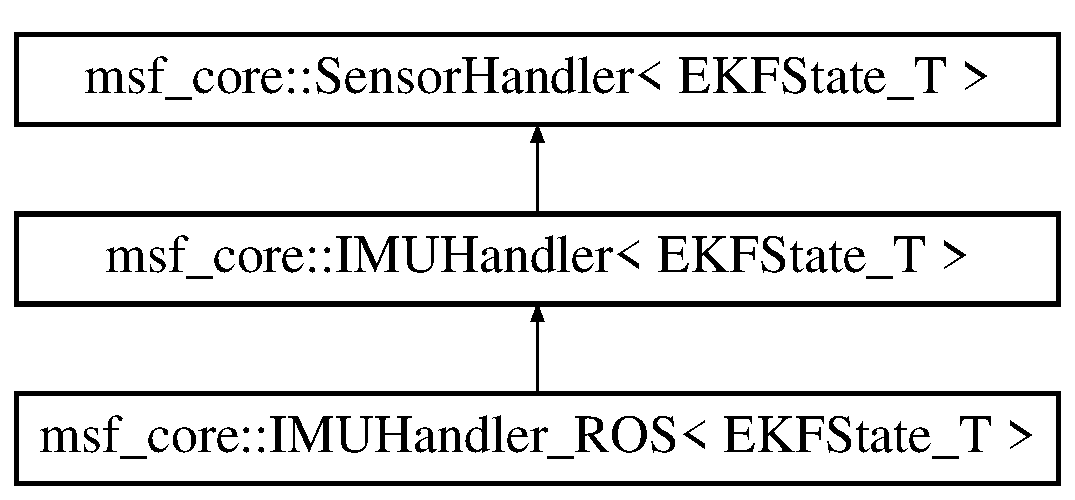
\includegraphics[height=3.000000cm]{classmsf__core_1_1IMUHandler}
\end{center}
\end{figure}
\subsection*{Public Member Functions}
\begin{DoxyCompactItemize}
\item 
\hyperlink{classmsf__core_1_1IMUHandler_a41084ec0130edd4c1b2934defbd19fb4}{I\-M\-U\-Handler} (\hyperlink{classmsf__core_1_1MSF__SensorManager}{M\-S\-F\-\_\-\-Sensor\-Manager}$<$ E\-K\-F\-State\-\_\-\-T $>$ \&mng, const std\-::string \&topic\-\_\-namespace, const std\-::string \&parameternamespace)
\item 
virtual \hyperlink{classmsf__core_1_1IMUHandler_a35cd9d86a2178b9ad85f00ebd598baa8}{$\sim$\-I\-M\-U\-Handler} ()
\item 
virtual bool \hyperlink{classmsf__core_1_1IMUHandler_aa343ee8a9375a7c3ecf9a980cf0bc82d}{initialize} ()=0
\item 
void \hyperlink{classmsf__core_1_1IMUHandler_a6b977a9a49ea5d91c5c61cb063169535}{process\-\_\-imu} (const msf\-\_\-core\-::\-Vector3 \&linear\-\_\-acceleration, const msf\-\_\-core\-::\-Vector3 \&angular\-\_\-velocity, const double \&msg\-\_\-stamp, size\-\_\-t msg\-\_\-seq)
\item 
void \hyperlink{classmsf__core_1_1IMUHandler_a46cd980264fb5369147c575a31f1dcb2}{process\-\_\-state} (const msf\-\_\-core\-::\-Vector3 \&linear\-\_\-acceleration, const msf\-\_\-core\-::\-Vector3 \&angular\-\_\-velocity, const msf\-\_\-core\-::\-Vector3 \&p, const msf\-\_\-core\-::\-Vector3 \&v, const \hyperlink{namespacemsf__core_a044c525dd7800e2e2f4bb86fc565a7c7}{msf\-\_\-core\-::\-Quaternion} \&q, bool is\-\_\-already\-\_\-propagated, const double \&msg\-\_\-stamp, size\-\_\-t msg\-\_\-seq)
\end{DoxyCompactItemize}
\subsection*{Protected Attributes}
\begin{DoxyCompactItemize}
\item 
shared\-\_\-ptr$<$ \hyperlink{classmsf__core_1_1MSF__Core}{M\-S\-F\-\_\-\-Core}\\*
$<$ E\-K\-F\-State\-\_\-\-T $>$ $>$ \hyperlink{classmsf__core_1_1IMUHandler_ae109422ae1b1ed7833bde860c71a9491}{core\-\_\-}
\end{DoxyCompactItemize}
\subsection*{Additional Inherited Members}


\subsection{Constructor \& Destructor Documentation}
\hypertarget{classmsf__core_1_1IMUHandler_a41084ec0130edd4c1b2934defbd19fb4}{\index{msf\-\_\-core\-::\-I\-M\-U\-Handler@{msf\-\_\-core\-::\-I\-M\-U\-Handler}!I\-M\-U\-Handler@{I\-M\-U\-Handler}}
\index{I\-M\-U\-Handler@{I\-M\-U\-Handler}!msf_core::IMUHandler@{msf\-\_\-core\-::\-I\-M\-U\-Handler}}
\subsubsection[{I\-M\-U\-Handler}]{\setlength{\rightskip}{0pt plus 5cm}template$<$typename E\-K\-F\-State\-\_\-\-T $>$ {\bf msf\-\_\-core\-::\-I\-M\-U\-Handler}$<$ E\-K\-F\-State\-\_\-\-T $>$\-::{\bf I\-M\-U\-Handler} (
\begin{DoxyParamCaption}
\item[{{\bf M\-S\-F\-\_\-\-Sensor\-Manager}$<$ E\-K\-F\-State\-\_\-\-T $>$ \&}]{mng, }
\item[{const std\-::string \&}]{topic\-\_\-namespace, }
\item[{const std\-::string \&}]{parameternamespace}
\end{DoxyParamCaption}
)\hspace{0.3cm}{\ttfamily [inline]}}}\label{classmsf__core_1_1IMUHandler_a41084ec0130edd4c1b2934defbd19fb4}
\hypertarget{classmsf__core_1_1IMUHandler_a35cd9d86a2178b9ad85f00ebd598baa8}{\index{msf\-\_\-core\-::\-I\-M\-U\-Handler@{msf\-\_\-core\-::\-I\-M\-U\-Handler}!$\sim$\-I\-M\-U\-Handler@{$\sim$\-I\-M\-U\-Handler}}
\index{$\sim$\-I\-M\-U\-Handler@{$\sim$\-I\-M\-U\-Handler}!msf_core::IMUHandler@{msf\-\_\-core\-::\-I\-M\-U\-Handler}}
\subsubsection[{$\sim$\-I\-M\-U\-Handler}]{\setlength{\rightskip}{0pt plus 5cm}template$<$typename E\-K\-F\-State\-\_\-\-T $>$ virtual {\bf msf\-\_\-core\-::\-I\-M\-U\-Handler}$<$ E\-K\-F\-State\-\_\-\-T $>$\-::$\sim${\bf I\-M\-U\-Handler} (
\begin{DoxyParamCaption}
{}
\end{DoxyParamCaption}
)\hspace{0.3cm}{\ttfamily [inline]}, {\ttfamily [virtual]}}}\label{classmsf__core_1_1IMUHandler_a35cd9d86a2178b9ad85f00ebd598baa8}


\subsection{Member Function Documentation}
\hypertarget{classmsf__core_1_1IMUHandler_aa343ee8a9375a7c3ecf9a980cf0bc82d}{\index{msf\-\_\-core\-::\-I\-M\-U\-Handler@{msf\-\_\-core\-::\-I\-M\-U\-Handler}!initialize@{initialize}}
\index{initialize@{initialize}!msf_core::IMUHandler@{msf\-\_\-core\-::\-I\-M\-U\-Handler}}
\subsubsection[{initialize}]{\setlength{\rightskip}{0pt plus 5cm}template$<$typename E\-K\-F\-State\-\_\-\-T $>$ virtual bool {\bf msf\-\_\-core\-::\-I\-M\-U\-Handler}$<$ E\-K\-F\-State\-\_\-\-T $>$\-::initialize (
\begin{DoxyParamCaption}
{}
\end{DoxyParamCaption}
)\hspace{0.3cm}{\ttfamily [pure virtual]}}}\label{classmsf__core_1_1IMUHandler_aa343ee8a9375a7c3ecf9a980cf0bc82d}


Implemented in \hyperlink{classmsf__core_1_1IMUHandler__ROS_ad620c283be06fad82e81903fc527564a}{msf\-\_\-core\-::\-I\-M\-U\-Handler\-\_\-\-R\-O\-S$<$ E\-K\-F\-State\-\_\-\-T $>$}.

\hypertarget{classmsf__core_1_1IMUHandler_a6b977a9a49ea5d91c5c61cb063169535}{\index{msf\-\_\-core\-::\-I\-M\-U\-Handler@{msf\-\_\-core\-::\-I\-M\-U\-Handler}!process\-\_\-imu@{process\-\_\-imu}}
\index{process\-\_\-imu@{process\-\_\-imu}!msf_core::IMUHandler@{msf\-\_\-core\-::\-I\-M\-U\-Handler}}
\subsubsection[{process\-\_\-imu}]{\setlength{\rightskip}{0pt plus 5cm}template$<$typename E\-K\-F\-State\-\_\-\-T $>$ void {\bf msf\-\_\-core\-::\-I\-M\-U\-Handler}$<$ E\-K\-F\-State\-\_\-\-T $>$\-::process\-\_\-imu (
\begin{DoxyParamCaption}
\item[{const msf\-\_\-core\-::\-Vector3 \&}]{linear\-\_\-acceleration, }
\item[{const msf\-\_\-core\-::\-Vector3 \&}]{angular\-\_\-velocity, }
\item[{const double \&}]{msg\-\_\-stamp, }
\item[{size\-\_\-t}]{msg\-\_\-seq}
\end{DoxyParamCaption}
)\hspace{0.3cm}{\ttfamily [inline]}}}\label{classmsf__core_1_1IMUHandler_a6b977a9a49ea5d91c5c61cb063169535}
\hypertarget{classmsf__core_1_1IMUHandler_a46cd980264fb5369147c575a31f1dcb2}{\index{msf\-\_\-core\-::\-I\-M\-U\-Handler@{msf\-\_\-core\-::\-I\-M\-U\-Handler}!process\-\_\-state@{process\-\_\-state}}
\index{process\-\_\-state@{process\-\_\-state}!msf_core::IMUHandler@{msf\-\_\-core\-::\-I\-M\-U\-Handler}}
\subsubsection[{process\-\_\-state}]{\setlength{\rightskip}{0pt plus 5cm}template$<$typename E\-K\-F\-State\-\_\-\-T $>$ void {\bf msf\-\_\-core\-::\-I\-M\-U\-Handler}$<$ E\-K\-F\-State\-\_\-\-T $>$\-::process\-\_\-state (
\begin{DoxyParamCaption}
\item[{const msf\-\_\-core\-::\-Vector3 \&}]{linear\-\_\-acceleration, }
\item[{const msf\-\_\-core\-::\-Vector3 \&}]{angular\-\_\-velocity, }
\item[{const msf\-\_\-core\-::\-Vector3 \&}]{p, }
\item[{const msf\-\_\-core\-::\-Vector3 \&}]{v, }
\item[{const {\bf msf\-\_\-core\-::\-Quaternion} \&}]{q, }
\item[{bool}]{is\-\_\-already\-\_\-propagated, }
\item[{const double \&}]{msg\-\_\-stamp, }
\item[{size\-\_\-t}]{msg\-\_\-seq}
\end{DoxyParamCaption}
)\hspace{0.3cm}{\ttfamily [inline]}}}\label{classmsf__core_1_1IMUHandler_a46cd980264fb5369147c575a31f1dcb2}


\subsection{Member Data Documentation}
\hypertarget{classmsf__core_1_1IMUHandler_ae109422ae1b1ed7833bde860c71a9491}{\index{msf\-\_\-core\-::\-I\-M\-U\-Handler@{msf\-\_\-core\-::\-I\-M\-U\-Handler}!core\-\_\-@{core\-\_\-}}
\index{core\-\_\-@{core\-\_\-}!msf_core::IMUHandler@{msf\-\_\-core\-::\-I\-M\-U\-Handler}}
\subsubsection[{core\-\_\-}]{\setlength{\rightskip}{0pt plus 5cm}template$<$typename E\-K\-F\-State\-\_\-\-T $>$ shared\-\_\-ptr$<${\bf M\-S\-F\-\_\-\-Core}$<$E\-K\-F\-State\-\_\-\-T$>$ $>$ {\bf msf\-\_\-core\-::\-I\-M\-U\-Handler}$<$ E\-K\-F\-State\-\_\-\-T $>$\-::core\-\_\-\hspace{0.3cm}{\ttfamily [protected]}}}\label{classmsf__core_1_1IMUHandler_ae109422ae1b1ed7833bde860c71a9491}


The documentation for this class was generated from the following file\-:\begin{DoxyCompactItemize}
\item 
msf\-\_\-core/include/msf\-\_\-core/\hyperlink{msf__IMUHandler_8h}{msf\-\_\-\-I\-M\-U\-Handler.\-h}\end{DoxyCompactItemize}

\hypertarget{classmsf__core_1_1IMUHandler__ROS}{\section{msf\-\_\-core\-:\-:I\-M\-U\-Handler\-\_\-\-R\-O\-S$<$ E\-K\-F\-State\-\_\-\-T $>$ Class Template Reference}
\label{classmsf__core_1_1IMUHandler__ROS}\index{msf\-\_\-core\-::\-I\-M\-U\-Handler\-\_\-\-R\-O\-S$<$ E\-K\-F\-State\-\_\-\-T $>$@{msf\-\_\-core\-::\-I\-M\-U\-Handler\-\_\-\-R\-O\-S$<$ E\-K\-F\-State\-\_\-\-T $>$}}
}


{\ttfamily \#include $<$msf\-\_\-\-I\-M\-U\-Handler\-\_\-\-R\-O\-S.\-h$>$}

Inheritance diagram for msf\-\_\-core\-:\-:I\-M\-U\-Handler\-\_\-\-R\-O\-S$<$ E\-K\-F\-State\-\_\-\-T $>$\-:\begin{figure}[H]
\begin{center}
\leavevmode
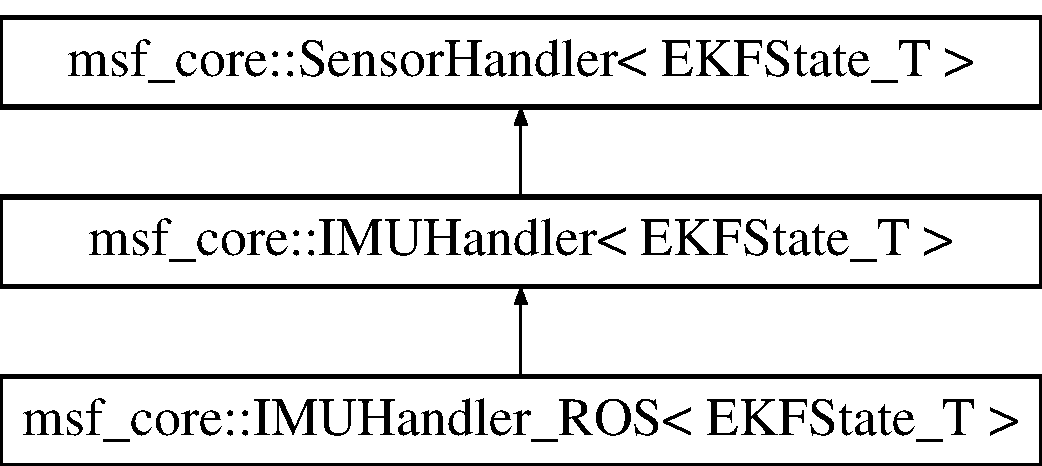
\includegraphics[height=3.000000cm]{classmsf__core_1_1IMUHandler__ROS}
\end{center}
\end{figure}
\subsection*{Public Member Functions}
\begin{DoxyCompactItemize}
\item 
\hyperlink{classmsf__core_1_1IMUHandler__ROS_ae5f7af48a65f50e446ac9286eaa162e8}{I\-M\-U\-Handler\-\_\-\-R\-O\-S} (\hyperlink{classmsf__core_1_1MSF__SensorManager}{M\-S\-F\-\_\-\-Sensor\-Manager}$<$ E\-K\-F\-State\-\_\-\-T $>$ \&mng, const std\-::string \&topic\-\_\-namespace, const std\-::string \&parameternamespace)
\item 
virtual \hyperlink{classmsf__core_1_1IMUHandler__ROS_a23c0a2175cbc4c5cc1f32f00cf08eeb1}{$\sim$\-I\-M\-U\-Handler\-\_\-\-R\-O\-S} ()
\item 
void \hyperlink{classmsf__core_1_1IMUHandler__ROS_a3ccc671b3e20d75c5b841c7834c94d9f}{state\-Callback} (const sensor\-\_\-fusion\-\_\-comm\-::\-Ext\-Ekf\-Const\-Ptr \&msg)
\item 
void \hyperlink{classmsf__core_1_1IMUHandler__ROS_a3d43bd281e85ad0c8efa9eb218be2913}{imu\-Callback\-\_\-asctec} (const asctec\-\_\-hl\-\_\-comm\-::mav\-\_\-imu\-Const\-Ptr \&msg)
\item 
void \hyperlink{classmsf__core_1_1IMUHandler__ROS_a11d2fecc4412b9664283d6e77fcaf31a}{imu\-Callback} (const sensor\-\_\-msgs\-::\-Imu\-Const\-Ptr \&msg)
\item 
virtual bool \hyperlink{classmsf__core_1_1IMUHandler__ROS_ad620c283be06fad82e81903fc527564a}{initialize} ()
\end{DoxyCompactItemize}
\subsection*{Private Attributes}
\begin{DoxyCompactItemize}
\item 
ros\-::\-Subscriber \hyperlink{classmsf__core_1_1IMUHandler__ROS_adf8d6fabf4ae2fffd11e82c6c8762f10}{sub\-State\-\_\-}
\begin{DoxyCompactList}\small\item\em subscriber to external state propagation \end{DoxyCompactList}\item 
ros\-::\-Subscriber \hyperlink{classmsf__core_1_1IMUHandler__ROS_a32b7e18f5fc3bf0a7de15ab8ca0bc9f9}{sub\-Imu\-\_\-}
\begin{DoxyCompactList}\small\item\em subscriber to I\-M\-U readings \end{DoxyCompactList}\item 
ros\-::\-Subscriber \hyperlink{classmsf__core_1_1IMUHandler__ROS_ac633011a1f63fc81b16972b3210bd4ec}{sub\-Imu\-Custom\-\_\-}
\begin{DoxyCompactList}\small\item\em subscriber to I\-M\-U readings for asctec custom \end{DoxyCompactList}\end{DoxyCompactItemize}
\subsection*{Additional Inherited Members}


\subsection{Constructor \& Destructor Documentation}
\hypertarget{classmsf__core_1_1IMUHandler__ROS_ae5f7af48a65f50e446ac9286eaa162e8}{\index{msf\-\_\-core\-::\-I\-M\-U\-Handler\-\_\-\-R\-O\-S@{msf\-\_\-core\-::\-I\-M\-U\-Handler\-\_\-\-R\-O\-S}!I\-M\-U\-Handler\-\_\-\-R\-O\-S@{I\-M\-U\-Handler\-\_\-\-R\-O\-S}}
\index{I\-M\-U\-Handler\-\_\-\-R\-O\-S@{I\-M\-U\-Handler\-\_\-\-R\-O\-S}!msf_core::IMUHandler_ROS@{msf\-\_\-core\-::\-I\-M\-U\-Handler\-\_\-\-R\-O\-S}}
\subsubsection[{I\-M\-U\-Handler\-\_\-\-R\-O\-S}]{\setlength{\rightskip}{0pt plus 5cm}template$<$typename E\-K\-F\-State\-\_\-\-T $>$ {\bf msf\-\_\-core\-::\-I\-M\-U\-Handler\-\_\-\-R\-O\-S}$<$ E\-K\-F\-State\-\_\-\-T $>$\-::{\bf I\-M\-U\-Handler\-\_\-\-R\-O\-S} (
\begin{DoxyParamCaption}
\item[{{\bf M\-S\-F\-\_\-\-Sensor\-Manager}$<$ E\-K\-F\-State\-\_\-\-T $>$ \&}]{mng, }
\item[{const std\-::string \&}]{topic\-\_\-namespace, }
\item[{const std\-::string \&}]{parameternamespace}
\end{DoxyParamCaption}
)\hspace{0.3cm}{\ttfamily [inline]}}}\label{classmsf__core_1_1IMUHandler__ROS_ae5f7af48a65f50e446ac9286eaa162e8}
\hypertarget{classmsf__core_1_1IMUHandler__ROS_a23c0a2175cbc4c5cc1f32f00cf08eeb1}{\index{msf\-\_\-core\-::\-I\-M\-U\-Handler\-\_\-\-R\-O\-S@{msf\-\_\-core\-::\-I\-M\-U\-Handler\-\_\-\-R\-O\-S}!$\sim$\-I\-M\-U\-Handler\-\_\-\-R\-O\-S@{$\sim$\-I\-M\-U\-Handler\-\_\-\-R\-O\-S}}
\index{$\sim$\-I\-M\-U\-Handler\-\_\-\-R\-O\-S@{$\sim$\-I\-M\-U\-Handler\-\_\-\-R\-O\-S}!msf_core::IMUHandler_ROS@{msf\-\_\-core\-::\-I\-M\-U\-Handler\-\_\-\-R\-O\-S}}
\subsubsection[{$\sim$\-I\-M\-U\-Handler\-\_\-\-R\-O\-S}]{\setlength{\rightskip}{0pt plus 5cm}template$<$typename E\-K\-F\-State\-\_\-\-T $>$ virtual {\bf msf\-\_\-core\-::\-I\-M\-U\-Handler\-\_\-\-R\-O\-S}$<$ E\-K\-F\-State\-\_\-\-T $>$\-::$\sim${\bf I\-M\-U\-Handler\-\_\-\-R\-O\-S} (
\begin{DoxyParamCaption}
{}
\end{DoxyParamCaption}
)\hspace{0.3cm}{\ttfamily [inline]}, {\ttfamily [virtual]}}}\label{classmsf__core_1_1IMUHandler__ROS_a23c0a2175cbc4c5cc1f32f00cf08eeb1}


\subsection{Member Function Documentation}
\hypertarget{classmsf__core_1_1IMUHandler__ROS_a11d2fecc4412b9664283d6e77fcaf31a}{\index{msf\-\_\-core\-::\-I\-M\-U\-Handler\-\_\-\-R\-O\-S@{msf\-\_\-core\-::\-I\-M\-U\-Handler\-\_\-\-R\-O\-S}!imu\-Callback@{imu\-Callback}}
\index{imu\-Callback@{imu\-Callback}!msf_core::IMUHandler_ROS@{msf\-\_\-core\-::\-I\-M\-U\-Handler\-\_\-\-R\-O\-S}}
\subsubsection[{imu\-Callback}]{\setlength{\rightskip}{0pt plus 5cm}template$<$typename E\-K\-F\-State\-\_\-\-T $>$ void {\bf msf\-\_\-core\-::\-I\-M\-U\-Handler\-\_\-\-R\-O\-S}$<$ E\-K\-F\-State\-\_\-\-T $>$\-::imu\-Callback (
\begin{DoxyParamCaption}
\item[{const sensor\-\_\-msgs\-::\-Imu\-Const\-Ptr \&}]{msg}
\end{DoxyParamCaption}
)\hspace{0.3cm}{\ttfamily [inline]}}}\label{classmsf__core_1_1IMUHandler__ROS_a11d2fecc4412b9664283d6e77fcaf31a}
\hypertarget{classmsf__core_1_1IMUHandler__ROS_a3d43bd281e85ad0c8efa9eb218be2913}{\index{msf\-\_\-core\-::\-I\-M\-U\-Handler\-\_\-\-R\-O\-S@{msf\-\_\-core\-::\-I\-M\-U\-Handler\-\_\-\-R\-O\-S}!imu\-Callback\-\_\-asctec@{imu\-Callback\-\_\-asctec}}
\index{imu\-Callback\-\_\-asctec@{imu\-Callback\-\_\-asctec}!msf_core::IMUHandler_ROS@{msf\-\_\-core\-::\-I\-M\-U\-Handler\-\_\-\-R\-O\-S}}
\subsubsection[{imu\-Callback\-\_\-asctec}]{\setlength{\rightskip}{0pt plus 5cm}template$<$typename E\-K\-F\-State\-\_\-\-T $>$ void {\bf msf\-\_\-core\-::\-I\-M\-U\-Handler\-\_\-\-R\-O\-S}$<$ E\-K\-F\-State\-\_\-\-T $>$\-::imu\-Callback\-\_\-asctec (
\begin{DoxyParamCaption}
\item[{const asctec\-\_\-hl\-\_\-comm\-::mav\-\_\-imu\-Const\-Ptr \&}]{msg}
\end{DoxyParamCaption}
)\hspace{0.3cm}{\ttfamily [inline]}}}\label{classmsf__core_1_1IMUHandler__ROS_a3d43bd281e85ad0c8efa9eb218be2913}
\hypertarget{classmsf__core_1_1IMUHandler__ROS_ad620c283be06fad82e81903fc527564a}{\index{msf\-\_\-core\-::\-I\-M\-U\-Handler\-\_\-\-R\-O\-S@{msf\-\_\-core\-::\-I\-M\-U\-Handler\-\_\-\-R\-O\-S}!initialize@{initialize}}
\index{initialize@{initialize}!msf_core::IMUHandler_ROS@{msf\-\_\-core\-::\-I\-M\-U\-Handler\-\_\-\-R\-O\-S}}
\subsubsection[{initialize}]{\setlength{\rightskip}{0pt plus 5cm}template$<$typename E\-K\-F\-State\-\_\-\-T $>$ virtual bool {\bf msf\-\_\-core\-::\-I\-M\-U\-Handler\-\_\-\-R\-O\-S}$<$ E\-K\-F\-State\-\_\-\-T $>$\-::initialize (
\begin{DoxyParamCaption}
{}
\end{DoxyParamCaption}
)\hspace{0.3cm}{\ttfamily [inline]}, {\ttfamily [virtual]}}}\label{classmsf__core_1_1IMUHandler__ROS_ad620c283be06fad82e81903fc527564a}


Implements \hyperlink{classmsf__core_1_1IMUHandler_aa343ee8a9375a7c3ecf9a980cf0bc82d}{msf\-\_\-core\-::\-I\-M\-U\-Handler$<$ E\-K\-F\-State\-\_\-\-T $>$}.

\hypertarget{classmsf__core_1_1IMUHandler__ROS_a3ccc671b3e20d75c5b841c7834c94d9f}{\index{msf\-\_\-core\-::\-I\-M\-U\-Handler\-\_\-\-R\-O\-S@{msf\-\_\-core\-::\-I\-M\-U\-Handler\-\_\-\-R\-O\-S}!state\-Callback@{state\-Callback}}
\index{state\-Callback@{state\-Callback}!msf_core::IMUHandler_ROS@{msf\-\_\-core\-::\-I\-M\-U\-Handler\-\_\-\-R\-O\-S}}
\subsubsection[{state\-Callback}]{\setlength{\rightskip}{0pt plus 5cm}template$<$typename E\-K\-F\-State\-\_\-\-T $>$ void {\bf msf\-\_\-core\-::\-I\-M\-U\-Handler\-\_\-\-R\-O\-S}$<$ E\-K\-F\-State\-\_\-\-T $>$\-::state\-Callback (
\begin{DoxyParamCaption}
\item[{const sensor\-\_\-fusion\-\_\-comm\-::\-Ext\-Ekf\-Const\-Ptr \&}]{msg}
\end{DoxyParamCaption}
)\hspace{0.3cm}{\ttfamily [inline]}}}\label{classmsf__core_1_1IMUHandler__ROS_a3ccc671b3e20d75c5b841c7834c94d9f}


\subsection{Member Data Documentation}
\hypertarget{classmsf__core_1_1IMUHandler__ROS_a32b7e18f5fc3bf0a7de15ab8ca0bc9f9}{\index{msf\-\_\-core\-::\-I\-M\-U\-Handler\-\_\-\-R\-O\-S@{msf\-\_\-core\-::\-I\-M\-U\-Handler\-\_\-\-R\-O\-S}!sub\-Imu\-\_\-@{sub\-Imu\-\_\-}}
\index{sub\-Imu\-\_\-@{sub\-Imu\-\_\-}!msf_core::IMUHandler_ROS@{msf\-\_\-core\-::\-I\-M\-U\-Handler\-\_\-\-R\-O\-S}}
\subsubsection[{sub\-Imu\-\_\-}]{\setlength{\rightskip}{0pt plus 5cm}template$<$typename E\-K\-F\-State\-\_\-\-T $>$ ros\-::\-Subscriber {\bf msf\-\_\-core\-::\-I\-M\-U\-Handler\-\_\-\-R\-O\-S}$<$ E\-K\-F\-State\-\_\-\-T $>$\-::sub\-Imu\-\_\-\hspace{0.3cm}{\ttfamily [private]}}}\label{classmsf__core_1_1IMUHandler__ROS_a32b7e18f5fc3bf0a7de15ab8ca0bc9f9}
\hypertarget{classmsf__core_1_1IMUHandler__ROS_ac633011a1f63fc81b16972b3210bd4ec}{\index{msf\-\_\-core\-::\-I\-M\-U\-Handler\-\_\-\-R\-O\-S@{msf\-\_\-core\-::\-I\-M\-U\-Handler\-\_\-\-R\-O\-S}!sub\-Imu\-Custom\-\_\-@{sub\-Imu\-Custom\-\_\-}}
\index{sub\-Imu\-Custom\-\_\-@{sub\-Imu\-Custom\-\_\-}!msf_core::IMUHandler_ROS@{msf\-\_\-core\-::\-I\-M\-U\-Handler\-\_\-\-R\-O\-S}}
\subsubsection[{sub\-Imu\-Custom\-\_\-}]{\setlength{\rightskip}{0pt plus 5cm}template$<$typename E\-K\-F\-State\-\_\-\-T $>$ ros\-::\-Subscriber {\bf msf\-\_\-core\-::\-I\-M\-U\-Handler\-\_\-\-R\-O\-S}$<$ E\-K\-F\-State\-\_\-\-T $>$\-::sub\-Imu\-Custom\-\_\-\hspace{0.3cm}{\ttfamily [private]}}}\label{classmsf__core_1_1IMUHandler__ROS_ac633011a1f63fc81b16972b3210bd4ec}
\hypertarget{classmsf__core_1_1IMUHandler__ROS_adf8d6fabf4ae2fffd11e82c6c8762f10}{\index{msf\-\_\-core\-::\-I\-M\-U\-Handler\-\_\-\-R\-O\-S@{msf\-\_\-core\-::\-I\-M\-U\-Handler\-\_\-\-R\-O\-S}!sub\-State\-\_\-@{sub\-State\-\_\-}}
\index{sub\-State\-\_\-@{sub\-State\-\_\-}!msf_core::IMUHandler_ROS@{msf\-\_\-core\-::\-I\-M\-U\-Handler\-\_\-\-R\-O\-S}}
\subsubsection[{sub\-State\-\_\-}]{\setlength{\rightskip}{0pt plus 5cm}template$<$typename E\-K\-F\-State\-\_\-\-T $>$ ros\-::\-Subscriber {\bf msf\-\_\-core\-::\-I\-M\-U\-Handler\-\_\-\-R\-O\-S}$<$ E\-K\-F\-State\-\_\-\-T $>$\-::sub\-State\-\_\-\hspace{0.3cm}{\ttfamily [private]}}}\label{classmsf__core_1_1IMUHandler__ROS_adf8d6fabf4ae2fffd11e82c6c8762f10}


The documentation for this class was generated from the following file\-:\begin{DoxyCompactItemize}
\item 
msf\-\_\-core/include/msf\-\_\-core/\hyperlink{msf__IMUHandler__ROS_8h}{msf\-\_\-\-I\-M\-U\-Handler\-\_\-\-R\-O\-S.\-h}\end{DoxyCompactItemize}

\hypertarget{structmsf__tmp_1_1IndexOfBestNonTemporalDriftingState}{\section{msf\-\_\-tmp\-:\-:Index\-Of\-Best\-Non\-Temporal\-Drifting\-State$<$ Sequence $>$ Struct Template Reference}
\label{structmsf__tmp_1_1IndexOfBestNonTemporalDriftingState}\index{msf\-\_\-tmp\-::\-Index\-Of\-Best\-Non\-Temporal\-Drifting\-State$<$ Sequence $>$@{msf\-\_\-tmp\-::\-Index\-Of\-Best\-Non\-Temporal\-Drifting\-State$<$ Sequence $>$}}
}


Find the best nontemporal drifting state in the full state vector at compile time.  




{\ttfamily \#include $<$msf\-\_\-tmp.\-h$>$}

\subsection*{Public Types}
\begin{DoxyCompactItemize}
\item 
enum \{ \hyperlink{structmsf__tmp_1_1IndexOfBestNonTemporalDriftingState_a8fc0a3f5c71a072f984cc9ad318ae803a83c8cb635dce2b45676d6997c1ee9a6f}{value}
 \}
\item 
typedef \\*
boost\-::fusion\-::result\-\_\-of\-::begin\\*
$<$ Sequence const  $>$\-::type \hyperlink{structmsf__tmp_1_1IndexOfBestNonTemporalDriftingState_a9f25e8cd8a466ed4bc97cd51b6a953e0}{First}
\item 
typedef \\*
boost\-::fusion\-::result\-\_\-of\-::end\\*
$<$ Sequence const  $>$\-::type \hyperlink{structmsf__tmp_1_1IndexOfBestNonTemporalDriftingState_a66dd8d7ca1fbe97b50c94896293c952f}{Last}
\end{DoxyCompactItemize}
\subsection*{Private Types}
\begin{DoxyCompactItemize}
\item 
enum \{ \hyperlink{structmsf__tmp_1_1IndexOfBestNonTemporalDriftingState_a5e3192e8bb76fae3485111504cb775cba9540152cd0cc657b1e5bfd4086b0005f}{bestindex} =  -\/1
 \}
\end{DoxyCompactItemize}
\subsection*{Private Member Functions}
\begin{DoxyCompactItemize}
\item 
\hyperlink{structmsf__tmp_1_1IndexOfBestNonTemporalDriftingState_ac45a91feef3e1c46195e14d44e7deef7}{static\-\_\-assert} (\hyperlink{structmsf__tmp_1_1CheckCorrectIndexing}{Check\-Correct\-Indexing}$<$ Sequence $>$\-::indexingerrors==0,\char`\"{}The \char`\"{}\char`\"{}indexing of the state vector is not the same as in the enum,\char`\"{}\char`\"{} but this must be the same\char`\"{})
\end{DoxyCompactItemize}


\subsection{Detailed Description}
\subsubsection*{template$<$typename Sequence$>$struct msf\-\_\-tmp\-::\-Index\-Of\-Best\-Non\-Temporal\-Drifting\-State$<$ Sequence $>$}

The goal of this tmp code is to find the best nontemporal drifting state in the full state vector at compile time. We therefore search the state variable list for states that the user has marked as non temporal drifting. If furthermore prefer quaternions over euclidean states. This function will return -\/1 if no suitable state has been found. 

\subsection{Member Typedef Documentation}
\hypertarget{structmsf__tmp_1_1IndexOfBestNonTemporalDriftingState_a9f25e8cd8a466ed4bc97cd51b6a953e0}{\index{msf\-\_\-tmp\-::\-Index\-Of\-Best\-Non\-Temporal\-Drifting\-State@{msf\-\_\-tmp\-::\-Index\-Of\-Best\-Non\-Temporal\-Drifting\-State}!First@{First}}
\index{First@{First}!msf_tmp::IndexOfBestNonTemporalDriftingState@{msf\-\_\-tmp\-::\-Index\-Of\-Best\-Non\-Temporal\-Drifting\-State}}
\subsubsection[{First}]{\setlength{\rightskip}{0pt plus 5cm}template$<$typename Sequence $>$ typedef boost\-::fusion\-::result\-\_\-of\-::begin$<$Sequence const$>$\-::type {\bf msf\-\_\-tmp\-::\-Index\-Of\-Best\-Non\-Temporal\-Drifting\-State}$<$ Sequence $>$\-::{\bf First}}}\label{structmsf__tmp_1_1IndexOfBestNonTemporalDriftingState_a9f25e8cd8a466ed4bc97cd51b6a953e0}
\hypertarget{structmsf__tmp_1_1IndexOfBestNonTemporalDriftingState_a66dd8d7ca1fbe97b50c94896293c952f}{\index{msf\-\_\-tmp\-::\-Index\-Of\-Best\-Non\-Temporal\-Drifting\-State@{msf\-\_\-tmp\-::\-Index\-Of\-Best\-Non\-Temporal\-Drifting\-State}!Last@{Last}}
\index{Last@{Last}!msf_tmp::IndexOfBestNonTemporalDriftingState@{msf\-\_\-tmp\-::\-Index\-Of\-Best\-Non\-Temporal\-Drifting\-State}}
\subsubsection[{Last}]{\setlength{\rightskip}{0pt plus 5cm}template$<$typename Sequence $>$ typedef boost\-::fusion\-::result\-\_\-of\-::end$<$Sequence const$>$\-::type {\bf msf\-\_\-tmp\-::\-Index\-Of\-Best\-Non\-Temporal\-Drifting\-State}$<$ Sequence $>$\-::{\bf Last}}}\label{structmsf__tmp_1_1IndexOfBestNonTemporalDriftingState_a66dd8d7ca1fbe97b50c94896293c952f}


\subsection{Member Enumeration Documentation}
\hypertarget{structmsf__tmp_1_1IndexOfBestNonTemporalDriftingState_a5e3192e8bb76fae3485111504cb775cb}{\subsubsection[{anonymous enum}]{\setlength{\rightskip}{0pt plus 5cm}template$<$typename Sequence $>$ anonymous enum\hspace{0.3cm}{\ttfamily [private]}}}\label{structmsf__tmp_1_1IndexOfBestNonTemporalDriftingState_a5e3192e8bb76fae3485111504cb775cb}
\begin{Desc}
\item[Enumerator\-: ]\par
\begin{description}
\index{bestindex@{bestindex}!msf\-\_\-tmp\-::\-Index\-Of\-Best\-Non\-Temporal\-Drifting\-State@{msf\-\_\-tmp\-::\-Index\-Of\-Best\-Non\-Temporal\-Drifting\-State}}\index{msf\-\_\-tmp\-::\-Index\-Of\-Best\-Non\-Temporal\-Drifting\-State@{msf\-\_\-tmp\-::\-Index\-Of\-Best\-Non\-Temporal\-Drifting\-State}!bestindex@{bestindex}}\item[{\em 
\hypertarget{structmsf__tmp_1_1IndexOfBestNonTemporalDriftingState_a5e3192e8bb76fae3485111504cb775cba9540152cd0cc657b1e5bfd4086b0005f}{bestindex}\label{structmsf__tmp_1_1IndexOfBestNonTemporalDriftingState_a5e3192e8bb76fae3485111504cb775cba9540152cd0cc657b1e5bfd4086b0005f}
}]\end{description}
\end{Desc}

\hypertarget{structmsf__tmp_1_1IndexOfBestNonTemporalDriftingState_a8fc0a3f5c71a072f984cc9ad318ae803}{\subsubsection[{anonymous enum}]{\setlength{\rightskip}{0pt plus 5cm}template$<$typename Sequence $>$ anonymous enum}}\label{structmsf__tmp_1_1IndexOfBestNonTemporalDriftingState_a8fc0a3f5c71a072f984cc9ad318ae803}
\begin{Desc}
\item[Enumerator\-: ]\par
\begin{description}
\index{value@{value}!msf\-\_\-tmp\-::\-Index\-Of\-Best\-Non\-Temporal\-Drifting\-State@{msf\-\_\-tmp\-::\-Index\-Of\-Best\-Non\-Temporal\-Drifting\-State}}\index{msf\-\_\-tmp\-::\-Index\-Of\-Best\-Non\-Temporal\-Drifting\-State@{msf\-\_\-tmp\-::\-Index\-Of\-Best\-Non\-Temporal\-Drifting\-State}!value@{value}}\item[{\em 
\hypertarget{structmsf__tmp_1_1IndexOfBestNonTemporalDriftingState_a8fc0a3f5c71a072f984cc9ad318ae803a83c8cb635dce2b45676d6997c1ee9a6f}{value}\label{structmsf__tmp_1_1IndexOfBestNonTemporalDriftingState_a8fc0a3f5c71a072f984cc9ad318ae803a83c8cb635dce2b45676d6997c1ee9a6f}
}]\end{description}
\end{Desc}



\subsection{Member Function Documentation}
\hypertarget{structmsf__tmp_1_1IndexOfBestNonTemporalDriftingState_ac45a91feef3e1c46195e14d44e7deef7}{\index{msf\-\_\-tmp\-::\-Index\-Of\-Best\-Non\-Temporal\-Drifting\-State@{msf\-\_\-tmp\-::\-Index\-Of\-Best\-Non\-Temporal\-Drifting\-State}!static\-\_\-assert@{static\-\_\-assert}}
\index{static\-\_\-assert@{static\-\_\-assert}!msf_tmp::IndexOfBestNonTemporalDriftingState@{msf\-\_\-tmp\-::\-Index\-Of\-Best\-Non\-Temporal\-Drifting\-State}}
\subsubsection[{static\-\_\-assert}]{\setlength{\rightskip}{0pt plus 5cm}template$<$typename Sequence $>$ {\bf msf\-\_\-tmp\-::\-Index\-Of\-Best\-Non\-Temporal\-Drifting\-State}$<$ Sequence $>$\-::static\-\_\-assert (
\begin{DoxyParamCaption}
\item[{{\bf Check\-Correct\-Indexing}$<$ Sequence $>$\-::indexingerrors}]{ = {\ttfamily =0}, }
\item[{\char`\"{}The \char`\"{}\char`\"{}indexing of the state vector is not the same as in the}]{enum, }
\item[{\char`\"{}\char`\"{}but this must be the same\char`\"{}}]{}
\end{DoxyParamCaption}
)\hspace{0.3cm}{\ttfamily [private]}}}\label{structmsf__tmp_1_1IndexOfBestNonTemporalDriftingState_ac45a91feef3e1c46195e14d44e7deef7}


The documentation for this struct was generated from the following file\-:\begin{DoxyCompactItemize}
\item 
msf\-\_\-core/include/msf\-\_\-core/\hyperlink{msf__tmp_8h}{msf\-\_\-tmp.\-h}\end{DoxyCompactItemize}

\hypertarget{structmsf__tmp_1_1IsPointerType}{\section{msf\-\_\-tmp\-:\-:Is\-Pointer\-Type$<$ T $>$ Struct Template Reference}
\label{structmsf__tmp_1_1IsPointerType}\index{msf\-\_\-tmp\-::\-Is\-Pointer\-Type$<$ T $>$@{msf\-\_\-tmp\-::\-Is\-Pointer\-Type$<$ T $>$}}
}


{\ttfamily \#include $<$msf\-\_\-typetraits.\-hpp$>$}

\subsection*{Public Types}
\begin{DoxyCompactItemize}
\item 
enum \{ \hyperlink{structmsf__tmp_1_1IsPointerType_a4ea953e50962ebf60bec8f1f5382ef11a34819f8f95b78509ba8558fc7f742db3}{value} =  false
 \}
\end{DoxyCompactItemize}


\subsection{Member Enumeration Documentation}
\hypertarget{structmsf__tmp_1_1IsPointerType_a4ea953e50962ebf60bec8f1f5382ef11}{\subsubsection[{anonymous enum}]{\setlength{\rightskip}{0pt plus 5cm}template$<$typename T $>$ anonymous enum}}\label{structmsf__tmp_1_1IsPointerType_a4ea953e50962ebf60bec8f1f5382ef11}
\begin{Desc}
\item[Enumerator\-: ]\par
\begin{description}
\index{value@{value}!msf\-\_\-tmp\-::\-Is\-Pointer\-Type@{msf\-\_\-tmp\-::\-Is\-Pointer\-Type}}\index{msf\-\_\-tmp\-::\-Is\-Pointer\-Type@{msf\-\_\-tmp\-::\-Is\-Pointer\-Type}!value@{value}}\item[{\em 
\hypertarget{structmsf__tmp_1_1IsPointerType_a4ea953e50962ebf60bec8f1f5382ef11a34819f8f95b78509ba8558fc7f742db3}{value}\label{structmsf__tmp_1_1IsPointerType_a4ea953e50962ebf60bec8f1f5382ef11a34819f8f95b78509ba8558fc7f742db3}
}]\end{description}
\end{Desc}



The documentation for this struct was generated from the following file\-:\begin{DoxyCompactItemize}
\item 
msf\-\_\-core/include/msf\-\_\-core/\hyperlink{msf__typetraits_8hpp}{msf\-\_\-typetraits.\-hpp}\end{DoxyCompactItemize}

\hypertarget{structmsf__tmp_1_1IsPointerType_3_01const_01T_01_5_01_4}{\section{msf\-\_\-tmp\-:\-:Is\-Pointer\-Type$<$ const T $\ast$ $>$ Struct Template Reference}
\label{structmsf__tmp_1_1IsPointerType_3_01const_01T_01_5_01_4}\index{msf\-\_\-tmp\-::\-Is\-Pointer\-Type$<$ const T $\ast$ $>$@{msf\-\_\-tmp\-::\-Is\-Pointer\-Type$<$ const T $\ast$ $>$}}
}


{\ttfamily \#include $<$msf\-\_\-typetraits.\-hpp$>$}

\subsection*{Public Types}
\begin{DoxyCompactItemize}
\item 
enum \{ \hyperlink{structmsf__tmp_1_1IsPointerType_3_01const_01T_01_5_01_4_a38756a8a0abddeb4f522af1c062c0b43a30cd53fda0de19c53837302ad8497f95}{value} =  true
 \}
\end{DoxyCompactItemize}


\subsection{Member Enumeration Documentation}
\hypertarget{structmsf__tmp_1_1IsPointerType_3_01const_01T_01_5_01_4_a38756a8a0abddeb4f522af1c062c0b43}{\subsubsection[{anonymous enum}]{\setlength{\rightskip}{0pt plus 5cm}template$<$typename T $>$ anonymous enum}}\label{structmsf__tmp_1_1IsPointerType_3_01const_01T_01_5_01_4_a38756a8a0abddeb4f522af1c062c0b43}
\begin{Desc}
\item[Enumerator\-: ]\par
\begin{description}
\index{value@{value}!msf\-\_\-tmp\-::\-Is\-Pointer\-Type$<$ const T $\ast$ $>$@{msf\-\_\-tmp\-::\-Is\-Pointer\-Type$<$ const T $\ast$ $>$}}\index{msf\-\_\-tmp\-::\-Is\-Pointer\-Type$<$ const T $\ast$ $>$@{msf\-\_\-tmp\-::\-Is\-Pointer\-Type$<$ const T $\ast$ $>$}!value@{value}}\item[{\em 
\hypertarget{structmsf__tmp_1_1IsPointerType_3_01const_01T_01_5_01_4_a38756a8a0abddeb4f522af1c062c0b43a30cd53fda0de19c53837302ad8497f95}{value}\label{structmsf__tmp_1_1IsPointerType_3_01const_01T_01_5_01_4_a38756a8a0abddeb4f522af1c062c0b43a30cd53fda0de19c53837302ad8497f95}
}]\end{description}
\end{Desc}



The documentation for this struct was generated from the following file\-:\begin{DoxyCompactItemize}
\item 
msf\-\_\-core/include/msf\-\_\-core/\hyperlink{msf__typetraits_8hpp}{msf\-\_\-typetraits.\-hpp}\end{DoxyCompactItemize}

\hypertarget{structmsf__tmp_1_1IsPointerType_3_01T_01_5_01_4}{\section{msf\-\_\-tmp\-:\-:Is\-Pointer\-Type$<$ T $\ast$ $>$ Struct Template Reference}
\label{structmsf__tmp_1_1IsPointerType_3_01T_01_5_01_4}\index{msf\-\_\-tmp\-::\-Is\-Pointer\-Type$<$ T $\ast$ $>$@{msf\-\_\-tmp\-::\-Is\-Pointer\-Type$<$ T $\ast$ $>$}}
}


{\ttfamily \#include $<$msf\-\_\-typetraits.\-hpp$>$}

\subsection*{Public Types}
\begin{DoxyCompactItemize}
\item 
enum \{ \hyperlink{structmsf__tmp_1_1IsPointerType_3_01T_01_5_01_4_ad3cce192490e61d2144ebf4be6808247a519f68be7a86d211fded991a71ad212a}{value} =  true
 \}
\end{DoxyCompactItemize}


\subsection{Member Enumeration Documentation}
\hypertarget{structmsf__tmp_1_1IsPointerType_3_01T_01_5_01_4_ad3cce192490e61d2144ebf4be6808247}{\subsubsection[{anonymous enum}]{\setlength{\rightskip}{0pt plus 5cm}template$<$typename T $>$ anonymous enum}}\label{structmsf__tmp_1_1IsPointerType_3_01T_01_5_01_4_ad3cce192490e61d2144ebf4be6808247}
\begin{Desc}
\item[Enumerator\-: ]\par
\begin{description}
\index{value@{value}!msf\-\_\-tmp\-::\-Is\-Pointer\-Type$<$ T $\ast$ $>$@{msf\-\_\-tmp\-::\-Is\-Pointer\-Type$<$ T $\ast$ $>$}}\index{msf\-\_\-tmp\-::\-Is\-Pointer\-Type$<$ T $\ast$ $>$@{msf\-\_\-tmp\-::\-Is\-Pointer\-Type$<$ T $\ast$ $>$}!value@{value}}\item[{\em 
\hypertarget{structmsf__tmp_1_1IsPointerType_3_01T_01_5_01_4_ad3cce192490e61d2144ebf4be6808247a519f68be7a86d211fded991a71ad212a}{value}\label{structmsf__tmp_1_1IsPointerType_3_01T_01_5_01_4_ad3cce192490e61d2144ebf4be6808247a519f68be7a86d211fded991a71ad212a}
}]\end{description}
\end{Desc}



The documentation for this struct was generated from the following file\-:\begin{DoxyCompactItemize}
\item 
msf\-\_\-core/include/msf\-\_\-core/\hyperlink{msf__typetraits_8hpp}{msf\-\_\-typetraits.\-hpp}\end{DoxyCompactItemize}

\hypertarget{structmsf__tmp_1_1IsReferenceType}{\section{msf\-\_\-tmp\-:\-:Is\-Reference\-Type$<$ T $>$ Struct Template Reference}
\label{structmsf__tmp_1_1IsReferenceType}\index{msf\-\_\-tmp\-::\-Is\-Reference\-Type$<$ T $>$@{msf\-\_\-tmp\-::\-Is\-Reference\-Type$<$ T $>$}}
}
\subsection*{Public Types}
\begin{DoxyCompactItemize}
\item 
enum \{ {\bfseries value} =  false
 \}
\end{DoxyCompactItemize}


The documentation for this struct was generated from the following file\-:\begin{DoxyCompactItemize}
\item 
msf\-\_\-core/include/msf\-\_\-core/msf\-\_\-typetraits.\-hpp\end{DoxyCompactItemize}

\hypertarget{structmsf__tmp_1_1IsReferenceType_3_01const_01T_01_6_01_4}{\section{msf\-\_\-tmp\-:\-:Is\-Reference\-Type$<$ const T \& $>$ Struct Template Reference}
\label{structmsf__tmp_1_1IsReferenceType_3_01const_01T_01_6_01_4}\index{msf\-\_\-tmp\-::\-Is\-Reference\-Type$<$ const T \& $>$@{msf\-\_\-tmp\-::\-Is\-Reference\-Type$<$ const T \& $>$}}
}
\subsection*{Public Types}
\begin{DoxyCompactItemize}
\item 
enum \{ {\bfseries value} =  true
 \}
\end{DoxyCompactItemize}


The documentation for this struct was generated from the following file\-:\begin{DoxyCompactItemize}
\item 
msf\-\_\-core/include/msf\-\_\-core/msf\-\_\-typetraits.\-hpp\end{DoxyCompactItemize}

\hypertarget{structmsf__tmp_1_1IsReferenceType_3_01T_01_6_01_4}{\section{msf\-\_\-tmp\-:\-:Is\-Reference\-Type$<$ T \& $>$ Struct Template Reference}
\label{structmsf__tmp_1_1IsReferenceType_3_01T_01_6_01_4}\index{msf\-\_\-tmp\-::\-Is\-Reference\-Type$<$ T \& $>$@{msf\-\_\-tmp\-::\-Is\-Reference\-Type$<$ T \& $>$}}
}
\subsection*{Public Types}
\begin{DoxyCompactItemize}
\item 
enum \{ {\bfseries value} =  true
 \}
\end{DoxyCompactItemize}


The documentation for this struct was generated from the following file\-:\begin{DoxyCompactItemize}
\item 
msf\-\_\-core/include/msf\-\_\-core/msf\-\_\-typetraits.\-hpp\end{DoxyCompactItemize}

\hypertarget{classmsf__core_1_1MSF__Core}{\section{msf\-\_\-core\-:\-:M\-S\-F\-\_\-\-Core$<$ E\-K\-F\-State\-\_\-\-T $>$ Class Template Reference}
\label{classmsf__core_1_1MSF__Core}\index{msf\-\_\-core\-::\-M\-S\-F\-\_\-\-Core$<$ E\-K\-F\-State\-\_\-\-T $>$@{msf\-\_\-core\-::\-M\-S\-F\-\_\-\-Core$<$ E\-K\-F\-State\-\_\-\-T $>$}}
}


The core class of the E\-K\-F Does propagation of state and covariance but also applying measurements and managing states and measurements in lists sorted by time stamp.  




{\ttfamily \#include $<$msf\-\_\-core.\-h$>$}

\subsection*{Public Types}
\begin{DoxyCompactItemize}
\item 
enum \{ \hyperlink{classmsf__core_1_1MSF__Core_a2bca35a2fba08b2fd5cc9963acc9c505afd5aaa703aae2fc6f022eec724b358f6}{n\-Error\-States\-At\-Compile\-Time} =  E\-K\-F\-State\-\_\-\-T\-:\-:n\-Error\-States\-At\-Compile\-Time, 
\hyperlink{classmsf__core_1_1MSF__Core_a2bca35a2fba08b2fd5cc9963acc9c505af1d75af5cfbf0cb1e0e9b04c5d944d6e}{n\-States\-At\-Compile\-Time} =  E\-K\-F\-State\-\_\-\-T\-:\-:n\-States\-At\-Compile\-Time
 \}
\item 
\hypertarget{classmsf__core_1_1MSF__Core_ace7a0e25e3945f3e84a6b16f72d1f1dd}{typedef \\*
E\-K\-F\-State\-\_\-\-T\-::\-State\-Definition\-\_\-\-T {\bfseries State\-Definition\-\_\-\-T}}\label{classmsf__core_1_1MSF__Core_ace7a0e25e3945f3e84a6b16f72d1f1dd}

\item 
\hypertarget{classmsf__core_1_1MSF__Core_af8de96f8f0a8677c79c12563f86b26d3}{typedef E\-K\-F\-State\-\_\-\-T\-::\-State\-Sequence\-\_\-\-T {\bfseries State\-Sequence\-\_\-\-T}}\label{classmsf__core_1_1MSF__Core_af8de96f8f0a8677c79c12563f86b26d3}

\item 
\hypertarget{classmsf__core_1_1MSF__Core_a01a15136971c11456e539f00b88fbf1a}{typedef Eigen\-::\-Matrix$<$ double, \\*
\hyperlink{classmsf__core_1_1MSF__Core_a2bca35a2fba08b2fd5cc9963acc9c505afd5aaa703aae2fc6f022eec724b358f6}{n\-Error\-States\-At\-Compile\-Time}, 1 $>$ \hyperlink{classmsf__core_1_1MSF__Core_a01a15136971c11456e539f00b88fbf1a}{Error\-State}}\label{classmsf__core_1_1MSF__Core_a01a15136971c11456e539f00b88fbf1a}

\begin{DoxyCompactList}\small\item\em The error state type. \end{DoxyCompactList}\item 
\hypertarget{classmsf__core_1_1MSF__Core_ad9b84aa4937f3c8354045b5c97ba2dcc}{typedef Eigen\-::\-Matrix$<$ double, \\*
\hyperlink{classmsf__core_1_1MSF__Core_a2bca35a2fba08b2fd5cc9963acc9c505afd5aaa703aae2fc6f022eec724b358f6}{n\-Error\-States\-At\-Compile\-Time}, \\*
\hyperlink{classmsf__core_1_1MSF__Core_a2bca35a2fba08b2fd5cc9963acc9c505afd5aaa703aae2fc6f022eec724b358f6}{n\-Error\-States\-At\-Compile\-Time} $>$ \hyperlink{classmsf__core_1_1MSF__Core_ad9b84aa4937f3c8354045b5c97ba2dcc}{Error\-State\-Cov}}\label{classmsf__core_1_1MSF__Core_ad9b84aa4937f3c8354045b5c97ba2dcc}

\begin{DoxyCompactList}\small\item\em The error state covariance type. \end{DoxyCompactList}\item 
\hypertarget{classmsf__core_1_1MSF__Core_a71db0f8ef9e865ef4d85b7365f01388d}{typedef \\*
\hyperlink{classmsf__core_1_1SortedContainer}{msf\-\_\-core\-::\-Sorted\-Container}\\*
$<$ E\-K\-F\-State\-\_\-\-T $>$ \hyperlink{classmsf__core_1_1MSF__Core_a71db0f8ef9e865ef4d85b7365f01388d}{State\-Buffer\-\_\-\-T}}\label{classmsf__core_1_1MSF__Core_a71db0f8ef9e865ef4d85b7365f01388d}

\begin{DoxyCompactList}\small\item\em The type of the state buffer containing all the states. \end{DoxyCompactList}\item 
\hypertarget{classmsf__core_1_1MSF__Core_abbdace8623ce8be7c430f6f7dad6b6fa}{typedef \\*
\hyperlink{classmsf__core_1_1SortedContainer}{msf\-\_\-core\-::\-Sorted\-Container}\\*
$<$ typename \\*
\hyperlink{classmsf__core_1_1MSF__MeasurementBase}{msf\-\_\-core\-::\-M\-S\-F\-\_\-\-Measurement\-Base}\\*
$<$ E\-K\-F\-State\-\_\-\-T $>$, typename \\*
\hyperlink{classmsf__core_1_1MSF__InvalidMeasurement}{msf\-\_\-core\-::\-M\-S\-F\-\_\-\-Invalid\-Measurement}\\*
$<$ E\-K\-F\-State\-\_\-\-T $>$ $>$ \hyperlink{classmsf__core_1_1MSF__Core_abbdace8623ce8be7c430f6f7dad6b6fa}{measurement\-Buffer\-T}}\label{classmsf__core_1_1MSF__Core_abbdace8623ce8be7c430f6f7dad6b6fa}

\begin{DoxyCompactList}\small\item\em The type of the measurement buffer containing all the measurements. \end{DoxyCompactList}\end{DoxyCompactItemize}
\subsection*{Public Member Functions}
\begin{DoxyCompactItemize}
\item 
void \hyperlink{classmsf__core_1_1MSF__Core_ac4b9bb4a30b0e1817a5cd07e843d6723}{add\-Measurement} (shared\-\_\-ptr$<$ \hyperlink{classmsf__core_1_1MSF__MeasurementBase}{M\-S\-F\-\_\-\-Measurement\-Base}$<$ E\-K\-F\-State\-\_\-\-T $>$ $>$ measurement)
\begin{DoxyCompactList}\small\item\em Add a sensor measurement or an init measurement to the internal queue and apply it to the state. \end{DoxyCompactList}\item 
void \hyperlink{classmsf__core_1_1MSF__Core_a68e27c538b3c7a255d1b5260ca00b52e}{init} (shared\-\_\-ptr$<$ \hyperlink{classmsf__core_1_1MSF__MeasurementBase}{M\-S\-F\-\_\-\-Measurement\-Base}$<$ E\-K\-F\-State\-\_\-\-T $>$ $>$ measurement)
\begin{DoxyCompactList}\small\item\em Initializes the filter with the values of the given measurement, other init values from other sensors can be passed in as \char`\"{}measurement\char`\"{} using the init\-Measurement structs. \end{DoxyCompactList}\item 
shared\-\_\-ptr$<$ E\-K\-F\-State\-\_\-\-T $>$ \hyperlink{classmsf__core_1_1MSF__Core_acc5117f9c7f79d9114a63033cbdeb9cb}{get\-Closest\-State} (double tstamp)
\begin{DoxyCompactList}\small\item\em Finds the closest state to the requested time in the internal state. \end{DoxyCompactList}\item 
\hypertarget{classmsf__core_1_1MSF__Core_af7d1cc22cc28fd4ccabda47cd2ff5888}{void \hyperlink{classmsf__core_1_1MSF__Core_af7d1cc22cc28fd4ccabda47cd2ff5888}{get\-Accum\-F\-\_\-\-S\-C} (const shared\-\_\-ptr$<$ E\-K\-F\-State\-\_\-\-T $>$ \&state\-\_\-old, const shared\-\_\-ptr$<$ E\-K\-F\-State\-\_\-\-T $>$ \&state\-\_\-new, Eigen\-::\-Matrix$<$ double, \hyperlink{classmsf__core_1_1MSF__Core_a2bca35a2fba08b2fd5cc9963acc9c505afd5aaa703aae2fc6f022eec724b358f6}{n\-Error\-States\-At\-Compile\-Time}, \hyperlink{classmsf__core_1_1MSF__Core_a2bca35a2fba08b2fd5cc9963acc9c505afd5aaa703aae2fc6f022eec724b358f6}{n\-Error\-States\-At\-Compile\-Time} $>$ \&F)}\label{classmsf__core_1_1MSF__Core_af7d1cc22cc28fd4ccabda47cd2ff5888}

\begin{DoxyCompactList}\small\item\em Returns the accumulated dynamic matrix between two states. \end{DoxyCompactList}\item 
\hypertarget{classmsf__core_1_1MSF__Core_a9c6b7908fbc66dd2aebb2f08e7c0c4ff}{shared\-\_\-ptr\\*
$<$ \hyperlink{classmsf__core_1_1MSF__MeasurementBase}{msf\-\_\-core\-::\-M\-S\-F\-\_\-\-Measurement\-Base}\\*
$<$ E\-K\-F\-State\-\_\-\-T $>$ $>$ \hyperlink{classmsf__core_1_1MSF__Core_a9c6b7908fbc66dd2aebb2f08e7c0c4ff}{get\-Previous\-Measurement} (double time, int sensor\-I\-D)}\label{classmsf__core_1_1MSF__Core_a9c6b7908fbc66dd2aebb2f08e7c0c4ff}

\begin{DoxyCompactList}\small\item\em Returns previous measurement of the same type. \end{DoxyCompactList}\item 
shared\-\_\-ptr$<$ E\-K\-F\-State\-\_\-\-T $>$ \hyperlink{classmsf__core_1_1MSF__Core_a759141ac2b7e8722e2c32a28490654fb}{get\-State\-At\-Time} (double tstamp)
\begin{DoxyCompactList}\small\item\em Finds the state at the requested time in the internal state. \end{DoxyCompactList}\item 
void \hyperlink{classmsf__core_1_1MSF__Core_aef8ea1eb9aedc8c196d4cc9a8411f77a}{predict\-Process\-Covariance} (shared\-\_\-ptr$<$ E\-K\-F\-State\-\_\-\-T $>$ \&state\-\_\-old, shared\-\_\-ptr$<$ E\-K\-F\-State\-\_\-\-T $>$ \&state\-\_\-new)
\begin{DoxyCompactList}\small\item\em Propagates the error state covariance. \end{DoxyCompactList}\item 
void \hyperlink{classmsf__core_1_1MSF__Core_a37342ed8ed1b25628ca423b20c95c9e0}{propagate\-State} (shared\-\_\-ptr$<$ E\-K\-F\-State\-\_\-\-T $>$ \&state\-\_\-old, shared\-\_\-ptr$<$ E\-K\-F\-State\-\_\-\-T $>$ \&state\-\_\-new)
\begin{DoxyCompactList}\small\item\em Propagates the state with given dt. \end{DoxyCompactList}\item 
\hypertarget{classmsf__core_1_1MSF__Core_ac5cd6f27e1965b7416bb4b847c72c2e6}{void \hyperlink{classmsf__core_1_1MSF__Core_ac5cd6f27e1965b7416bb4b847c72c2e6}{Clean\-Up\-Buffers} ()}\label{classmsf__core_1_1MSF__Core_ac5cd6f27e1965b7416bb4b847c72c2e6}

\begin{DoxyCompactList}\small\item\em Delete very old states and measurements from the buffers to free memory. \end{DoxyCompactList}\item 
void \hyperlink{classmsf__core_1_1MSF__Core_a5f520250e12d56a8950f4fc355e58d69}{set\-P\-Core} (Eigen\-::\-Matrix$<$ double, E\-K\-F\-State\-\_\-\-T\-::n\-Error\-States\-At\-Compile\-Time, E\-K\-F\-State\-\_\-\-T\-::n\-Error\-States\-At\-Compile\-Time $>$ \&P)
\begin{DoxyCompactList}\small\item\em sets the covariance matrix of the core states to simulated values. \end{DoxyCompactList}\item 
\hyperlink{classmsf__core_1_1MSF__Core_ad55343b1396263b7a1f2b5599d0fc4e0}{M\-S\-F\-\_\-\-Core} (const \hyperlink{classmsf__core_1_1MSF__SensorManager}{M\-S\-F\-\_\-\-Sensor\-Manager}$<$ E\-K\-F\-State\-\_\-\-T $>$ \&usercalc)
\begin{DoxyCompactList}\small\item\em Ctor takes a pointer to an object which does the user defined calculations and provides interfaces for initialization etc. \end{DoxyCompactList}\item 
\hypertarget{classmsf__core_1_1MSF__Core_a4685230ba43fd684aaf6d6b891c29fca}{const \hyperlink{classmsf__core_1_1MSF__SensorManager}{M\-S\-F\-\_\-\-Sensor\-Manager}\\*
$<$ E\-K\-F\-State\-\_\-\-T $>$ \& {\bfseries usercalc} () const }\label{classmsf__core_1_1MSF__Core_a4685230ba43fd684aaf6d6b891c29fca}

\end{DoxyCompactItemize}
\subsection*{Public Attributes}
\begin{DoxyCompactItemize}
\item 
\hypertarget{classmsf__core_1_1MSF__Core_aad8769aeb9efa04de99604dd397a47a8}{{\bfseries E\-I\-G\-E\-N\-\_\-\-M\-A\-K\-E\-\_\-\-A\-L\-I\-G\-N\-E\-D\-\_\-\-O\-P\-E\-R\-A\-T\-O\-R\-\_\-\-N\-E\-W}}\label{classmsf__core_1_1MSF__Core_aad8769aeb9efa04de99604dd397a47a8}

\end{DoxyCompactItemize}
\subsection*{Friends}
\begin{DoxyCompactItemize}
\item 
\hypertarget{classmsf__core_1_1MSF__Core_a096bb61133872bdd266587ce54e931e6}{class {\bfseries M\-S\-F\-\_\-\-Measurement\-Base$<$ E\-K\-F\-State\-\_\-\-T $>$}}\label{classmsf__core_1_1MSF__Core_a096bb61133872bdd266587ce54e931e6}

\item 
\hypertarget{classmsf__core_1_1MSF__Core_a868b4fae6ec6ad5b5ae95d1980ac1704}{class {\bfseries I\-M\-U\-Handler$<$ E\-K\-F\-State\-\_\-\-T $>$}}\label{classmsf__core_1_1MSF__Core_a868b4fae6ec6ad5b5ae95d1980ac1704}

\end{DoxyCompactItemize}


\subsection{Detailed Description}
\subsubsection*{template$<$typename E\-K\-F\-State\-\_\-\-T$>$class msf\-\_\-core\-::\-M\-S\-F\-\_\-\-Core$<$ E\-K\-F\-State\-\_\-\-T $>$}

The core class of the E\-K\-F Does propagation of state and covariance but also applying measurements and managing states and measurements in lists sorted by time stamp. 

\subsection{Member Enumeration Documentation}
\hypertarget{classmsf__core_1_1MSF__Core_a2bca35a2fba08b2fd5cc9963acc9c505}{\subsubsection[{anonymous enum}]{\setlength{\rightskip}{0pt plus 5cm}template$<$typename E\-K\-F\-State\-\_\-\-T$>$ anonymous enum}}\label{classmsf__core_1_1MSF__Core_a2bca35a2fba08b2fd5cc9963acc9c505}
\begin{Desc}
\item[Enumerator\-: ]\par
\begin{description}
\index{n\-Error\-States\-At\-Compile\-Time@{n\-Error\-States\-At\-Compile\-Time}!msf\-\_\-core\-::\-M\-S\-F\-\_\-\-Core@{msf\-\_\-core\-::\-M\-S\-F\-\_\-\-Core}}\index{msf\-\_\-core\-::\-M\-S\-F\-\_\-\-Core@{msf\-\_\-core\-::\-M\-S\-F\-\_\-\-Core}!n\-Error\-States\-At\-Compile\-Time@{n\-Error\-States\-At\-Compile\-Time}}\item[{\em 
\hypertarget{classmsf__core_1_1MSF__Core_a2bca35a2fba08b2fd5cc9963acc9c505afd5aaa703aae2fc6f022eec724b358f6}{n\-Error\-States\-At\-Compile\-Time}\label{classmsf__core_1_1MSF__Core_a2bca35a2fba08b2fd5cc9963acc9c505afd5aaa703aae2fc6f022eec724b358f6}
}]Error state length. \index{n\-States\-At\-Compile\-Time@{n\-States\-At\-Compile\-Time}!msf\-\_\-core\-::\-M\-S\-F\-\_\-\-Core@{msf\-\_\-core\-::\-M\-S\-F\-\_\-\-Core}}\index{msf\-\_\-core\-::\-M\-S\-F\-\_\-\-Core@{msf\-\_\-core\-::\-M\-S\-F\-\_\-\-Core}!n\-States\-At\-Compile\-Time@{n\-States\-At\-Compile\-Time}}\item[{\em 
\hypertarget{classmsf__core_1_1MSF__Core_a2bca35a2fba08b2fd5cc9963acc9c505af1d75af5cfbf0cb1e0e9b04c5d944d6e}{n\-States\-At\-Compile\-Time}\label{classmsf__core_1_1MSF__Core_a2bca35a2fba08b2fd5cc9963acc9c505af1d75af5cfbf0cb1e0e9b04c5d944d6e}
}]Complete state length. \end{description}
\end{Desc}



\subsection{Constructor \& Destructor Documentation}
\hypertarget{classmsf__core_1_1MSF__Core_ad55343b1396263b7a1f2b5599d0fc4e0}{\index{msf\-\_\-core\-::\-M\-S\-F\-\_\-\-Core@{msf\-\_\-core\-::\-M\-S\-F\-\_\-\-Core}!M\-S\-F\-\_\-\-Core@{M\-S\-F\-\_\-\-Core}}
\index{M\-S\-F\-\_\-\-Core@{M\-S\-F\-\_\-\-Core}!msf_core::MSF_Core@{msf\-\_\-core\-::\-M\-S\-F\-\_\-\-Core}}
\subsubsection[{M\-S\-F\-\_\-\-Core}]{\setlength{\rightskip}{0pt plus 5cm}template$<$typename E\-K\-F\-State\-\_\-\-T $>$ {\bf msf\-\_\-core\-::\-M\-S\-F\-\_\-\-Core}$<$ E\-K\-F\-State\-\_\-\-T $>$\-::{\bf M\-S\-F\-\_\-\-Core} (
\begin{DoxyParamCaption}
\item[{const {\bf M\-S\-F\-\_\-\-Sensor\-Manager}$<$ E\-K\-F\-State\-\_\-\-T $>$ \&}]{usercalc}
\end{DoxyParamCaption}
)}}\label{classmsf__core_1_1MSF__Core_ad55343b1396263b7a1f2b5599d0fc4e0}


Ctor takes a pointer to an object which does the user defined calculations and provides interfaces for initialization etc. 


\begin{DoxyParams}{Parameters}
{\em usercalc} & The class providing the user defined calculations D\-O A\-B\-S\-O\-L\-U\-T\-E\-L\-Y N\-O\-T U\-S\-E T\-H\-I\-S R\-E\-F\-E\-R\-E\-N\-C\-E I\-N\-S\-I\-D\-E T\-H\-I\-S C\-T\-O\-R!! \\
\hline
\end{DoxyParams}


\subsection{Member Function Documentation}
\hypertarget{classmsf__core_1_1MSF__Core_ac4b9bb4a30b0e1817a5cd07e843d6723}{\index{msf\-\_\-core\-::\-M\-S\-F\-\_\-\-Core@{msf\-\_\-core\-::\-M\-S\-F\-\_\-\-Core}!add\-Measurement@{add\-Measurement}}
\index{add\-Measurement@{add\-Measurement}!msf_core::MSF_Core@{msf\-\_\-core\-::\-M\-S\-F\-\_\-\-Core}}
\subsubsection[{add\-Measurement}]{\setlength{\rightskip}{0pt plus 5cm}template$<$typename E\-K\-F\-State\-\_\-\-T $>$ void {\bf msf\-\_\-core\-::\-M\-S\-F\-\_\-\-Core}$<$ E\-K\-F\-State\-\_\-\-T $>$\-::add\-Measurement (
\begin{DoxyParamCaption}
\item[{shared\-\_\-ptr$<$ {\bf M\-S\-F\-\_\-\-Measurement\-Base}$<$ E\-K\-F\-State\-\_\-\-T $>$ $>$}]{measurement}
\end{DoxyParamCaption}
)}}\label{classmsf__core_1_1MSF__Core_ac4b9bb4a30b0e1817a5cd07e843d6723}


Add a sensor measurement or an init measurement to the internal queue and apply it to the state. 


\begin{DoxyParams}{Parameters}
{\em Measurement} & the measurement to add to the internal measurement queue. \\
\hline
\end{DoxyParams}
\hypertarget{classmsf__core_1_1MSF__Core_acc5117f9c7f79d9114a63033cbdeb9cb}{\index{msf\-\_\-core\-::\-M\-S\-F\-\_\-\-Core@{msf\-\_\-core\-::\-M\-S\-F\-\_\-\-Core}!get\-Closest\-State@{get\-Closest\-State}}
\index{get\-Closest\-State@{get\-Closest\-State}!msf_core::MSF_Core@{msf\-\_\-core\-::\-M\-S\-F\-\_\-\-Core}}
\subsubsection[{get\-Closest\-State}]{\setlength{\rightskip}{0pt plus 5cm}template$<$typename E\-K\-F\-State\-\_\-\-T $>$ shared\-\_\-ptr$<$ E\-K\-F\-State\-\_\-\-T $>$ {\bf msf\-\_\-core\-::\-M\-S\-F\-\_\-\-Core}$<$ E\-K\-F\-State\-\_\-\-T $>$\-::get\-Closest\-State (
\begin{DoxyParamCaption}
\item[{double}]{tstamp}
\end{DoxyParamCaption}
)}}\label{classmsf__core_1_1MSF__Core_acc5117f9c7f79d9114a63033cbdeb9cb}


Finds the closest state to the requested time in the internal state. 


\begin{DoxyParams}{Parameters}
{\em tstamp} & The time stamp to find the closest state to. \\
\hline
\end{DoxyParams}
\hypertarget{classmsf__core_1_1MSF__Core_a759141ac2b7e8722e2c32a28490654fb}{\index{msf\-\_\-core\-::\-M\-S\-F\-\_\-\-Core@{msf\-\_\-core\-::\-M\-S\-F\-\_\-\-Core}!get\-State\-At\-Time@{get\-State\-At\-Time}}
\index{get\-State\-At\-Time@{get\-State\-At\-Time}!msf_core::MSF_Core@{msf\-\_\-core\-::\-M\-S\-F\-\_\-\-Core}}
\subsubsection[{get\-State\-At\-Time}]{\setlength{\rightskip}{0pt plus 5cm}template$<$typename E\-K\-F\-State\-\_\-\-T $>$ shared\-\_\-ptr$<$ E\-K\-F\-State\-\_\-\-T $>$ {\bf msf\-\_\-core\-::\-M\-S\-F\-\_\-\-Core}$<$ E\-K\-F\-State\-\_\-\-T $>$\-::get\-State\-At\-Time (
\begin{DoxyParamCaption}
\item[{double}]{tstamp}
\end{DoxyParamCaption}
)}}\label{classmsf__core_1_1MSF__Core_a759141ac2b7e8722e2c32a28490654fb}


Finds the state at the requested time in the internal state. 


\begin{DoxyParams}{Parameters}
{\em tstamp} & The time stamp to find the state to. \\
\hline
\end{DoxyParams}
\hypertarget{classmsf__core_1_1MSF__Core_a68e27c538b3c7a255d1b5260ca00b52e}{\index{msf\-\_\-core\-::\-M\-S\-F\-\_\-\-Core@{msf\-\_\-core\-::\-M\-S\-F\-\_\-\-Core}!init@{init}}
\index{init@{init}!msf_core::MSF_Core@{msf\-\_\-core\-::\-M\-S\-F\-\_\-\-Core}}
\subsubsection[{init}]{\setlength{\rightskip}{0pt plus 5cm}template$<$typename E\-K\-F\-State\-\_\-\-T $>$ void {\bf msf\-\_\-core\-::\-M\-S\-F\-\_\-\-Core}$<$ E\-K\-F\-State\-\_\-\-T $>$\-::init (
\begin{DoxyParamCaption}
\item[{shared\-\_\-ptr$<$ {\bf M\-S\-F\-\_\-\-Measurement\-Base}$<$ E\-K\-F\-State\-\_\-\-T $>$ $>$}]{measurement}
\end{DoxyParamCaption}
)}}\label{classmsf__core_1_1MSF__Core_a68e27c538b3c7a255d1b5260ca00b52e}


Initializes the filter with the values of the given measurement, other init values from other sensors can be passed in as \char`\"{}measurement\char`\"{} using the init\-Measurement structs. 


\begin{DoxyParams}{Parameters}
{\em Measurement} & a measurement containing initial values for the state \\
\hline
\end{DoxyParams}
\hypertarget{classmsf__core_1_1MSF__Core_aef8ea1eb9aedc8c196d4cc9a8411f77a}{\index{msf\-\_\-core\-::\-M\-S\-F\-\_\-\-Core@{msf\-\_\-core\-::\-M\-S\-F\-\_\-\-Core}!predict\-Process\-Covariance@{predict\-Process\-Covariance}}
\index{predict\-Process\-Covariance@{predict\-Process\-Covariance}!msf_core::MSF_Core@{msf\-\_\-core\-::\-M\-S\-F\-\_\-\-Core}}
\subsubsection[{predict\-Process\-Covariance}]{\setlength{\rightskip}{0pt plus 5cm}template$<$typename E\-K\-F\-State\-\_\-\-T $>$ void {\bf msf\-\_\-core\-::\-M\-S\-F\-\_\-\-Core}$<$ E\-K\-F\-State\-\_\-\-T $>$\-::predict\-Process\-Covariance (
\begin{DoxyParamCaption}
\item[{shared\-\_\-ptr$<$ E\-K\-F\-State\-\_\-\-T $>$ \&}]{state\-\_\-old, }
\item[{shared\-\_\-ptr$<$ E\-K\-F\-State\-\_\-\-T $>$ \&}]{state\-\_\-new}
\end{DoxyParamCaption}
)}}\label{classmsf__core_1_1MSF__Core_aef8ea1eb9aedc8c196d4cc9a8411f77a}


Propagates the error state covariance. 


\begin{DoxyParams}{Parameters}
{\em state\-\_\-old} & The state to propagate the covariance from. \\
\hline
{\em state\-\_\-new} & The state to propagate the covariance to. \\
\hline
\end{DoxyParams}
\hypertarget{classmsf__core_1_1MSF__Core_a37342ed8ed1b25628ca423b20c95c9e0}{\index{msf\-\_\-core\-::\-M\-S\-F\-\_\-\-Core@{msf\-\_\-core\-::\-M\-S\-F\-\_\-\-Core}!propagate\-State@{propagate\-State}}
\index{propagate\-State@{propagate\-State}!msf_core::MSF_Core@{msf\-\_\-core\-::\-M\-S\-F\-\_\-\-Core}}
\subsubsection[{propagate\-State}]{\setlength{\rightskip}{0pt plus 5cm}template$<$typename E\-K\-F\-State\-\_\-\-T $>$ void {\bf msf\-\_\-core\-::\-M\-S\-F\-\_\-\-Core}$<$ E\-K\-F\-State\-\_\-\-T $>$\-::propagate\-State (
\begin{DoxyParamCaption}
\item[{shared\-\_\-ptr$<$ E\-K\-F\-State\-\_\-\-T $>$ \&}]{state\-\_\-old, }
\item[{shared\-\_\-ptr$<$ E\-K\-F\-State\-\_\-\-T $>$ \&}]{state\-\_\-new}
\end{DoxyParamCaption}
)}}\label{classmsf__core_1_1MSF__Core_a37342ed8ed1b25628ca423b20c95c9e0}


Propagates the state with given dt. 


\begin{DoxyParams}{Parameters}
{\em state\-\_\-old} & The state to propagate from. \\
\hline
{\em state\-\_\-new} & The state to propagate to. \\
\hline
\end{DoxyParams}
\hypertarget{classmsf__core_1_1MSF__Core_a5f520250e12d56a8950f4fc355e58d69}{\index{msf\-\_\-core\-::\-M\-S\-F\-\_\-\-Core@{msf\-\_\-core\-::\-M\-S\-F\-\_\-\-Core}!set\-P\-Core@{set\-P\-Core}}
\index{set\-P\-Core@{set\-P\-Core}!msf_core::MSF_Core@{msf\-\_\-core\-::\-M\-S\-F\-\_\-\-Core}}
\subsubsection[{set\-P\-Core}]{\setlength{\rightskip}{0pt plus 5cm}template$<$typename E\-K\-F\-State\-\_\-\-T $>$ void {\bf msf\-\_\-core\-::\-M\-S\-F\-\_\-\-Core}$<$ E\-K\-F\-State\-\_\-\-T $>$\-::set\-P\-Core (
\begin{DoxyParamCaption}
\item[{Eigen\-::\-Matrix$<$ double, E\-K\-F\-State\-\_\-\-T\-::n\-Error\-States\-At\-Compile\-Time, E\-K\-F\-State\-\_\-\-T\-::n\-Error\-States\-At\-Compile\-Time $>$ \&}]{P}
\end{DoxyParamCaption}
)}}\label{classmsf__core_1_1MSF__Core_a5f520250e12d56a8950f4fc355e58d69}


sets the covariance matrix of the core states to simulated values. 


\begin{DoxyParams}{Parameters}
{\em P} & the error state covariance Matrix to fill. \\
\hline
\end{DoxyParams}


The documentation for this class was generated from the following files\-:\begin{DoxyCompactItemize}
\item 
msf\-\_\-core/include/msf\-\_\-core/msf\-\_\-core.\-h\item 
msf\-\_\-core/include/msf\-\_\-core/implementation/msf\-\_\-core.\-hpp\end{DoxyCompactItemize}

\hypertarget{classmsf__core_1_1MSF__InitMeasurement}{\section{msf\-\_\-core\-:\-:M\-S\-F\-\_\-\-Init\-Measurement$<$ E\-K\-F\-State\-\_\-\-T $>$ Class Template Reference}
\label{classmsf__core_1_1MSF__InitMeasurement}\index{msf\-\_\-core\-::\-M\-S\-F\-\_\-\-Init\-Measurement$<$ E\-K\-F\-State\-\_\-\-T $>$@{msf\-\_\-core\-::\-M\-S\-F\-\_\-\-Init\-Measurement$<$ E\-K\-F\-State\-\_\-\-T $>$}}
}


A measurement to be send to initialize parts of or the full E\-K\-F state this can especially be used to split the initialization of the E\-K\-F between multiple sensors which init different parts of the state.  




{\ttfamily \#include $<$msf\-\_\-measurement.\-h$>$}

Inheritance diagram for msf\-\_\-core\-:\-:M\-S\-F\-\_\-\-Init\-Measurement$<$ E\-K\-F\-State\-\_\-\-T $>$\-:\begin{figure}[H]
\begin{center}
\leavevmode
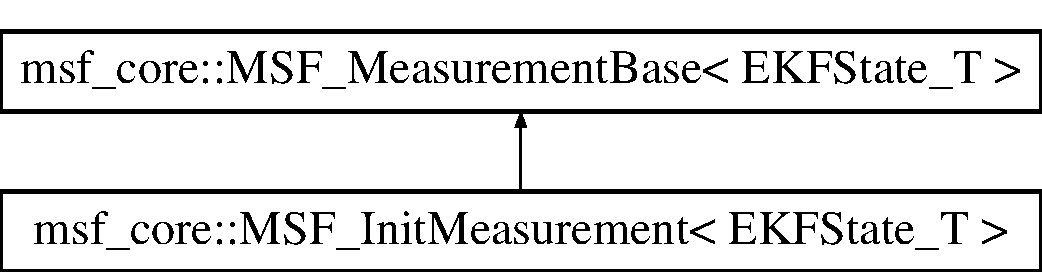
\includegraphics[height=2.000000cm]{classmsf__core_1_1MSF__InitMeasurement}
\end{center}
\end{figure}
\subsection*{Public Member Functions}
\begin{DoxyCompactItemize}
\item 
\hypertarget{classmsf__core_1_1MSF__InitMeasurement_aaa7c4e7ea351aae40daa3ce32fb37e58}{E\-I\-G\-E\-N\-\_\-\-M\-A\-K\-E\-\_\-\-A\-L\-I\-G\-N\-E\-D\-\_\-\-O\-P\-E\-R\-A\-T\-O\-R\-\_\-\-N\-E\-W {\bfseries M\-S\-F\-\_\-\-Init\-Measurement} (bool Contains\-Initial\-Sensor\-Readings)}\label{classmsf__core_1_1MSF__InitMeasurement_aaa7c4e7ea351aae40daa3ce32fb37e58}

\item 
\hypertarget{classmsf__core_1_1MSF__InitMeasurement_a6ade2a1ba88e5f26de2125258e4c5238}{virtual std\-::string {\bfseries type} ()}\label{classmsf__core_1_1MSF__InitMeasurement_a6ade2a1ba88e5f26de2125258e4c5238}

\item 
\hypertarget{classmsf__core_1_1MSF__InitMeasurement_a19cc3b1efefda7694cca93d1bae441f5}{E\-K\-F\-State\-\_\-\-T\-::\-P\-\_\-type \& {\bfseries get\-\_\-\-P} ()}\label{classmsf__core_1_1MSF__InitMeasurement_a19cc3b1efefda7694cca93d1bae441f5}

\item 
\hypertarget{classmsf__core_1_1MSF__InitMeasurement_af0c9a4a740bc019d8a6a223d469bb42f}{Eigen\-::\-Matrix$<$ double, 3, 1 $>$ \& \hyperlink{classmsf__core_1_1MSF__InitMeasurement_af0c9a4a740bc019d8a6a223d469bb42f}{get\-\_\-w\-\_\-m} ()}\label{classmsf__core_1_1MSF__InitMeasurement_af0c9a4a740bc019d8a6a223d469bb42f}

\begin{DoxyCompactList}\small\item\em Get the gyro measurement. \end{DoxyCompactList}\item 
\hypertarget{classmsf__core_1_1MSF__InitMeasurement_a4c2c7250787e58868c9fc9596ed4c217}{Eigen\-::\-Matrix$<$ double, 3, 1 $>$ \& \hyperlink{classmsf__core_1_1MSF__InitMeasurement_a4c2c7250787e58868c9fc9596ed4c217}{get\-\_\-a\-\_\-m} ()}\label{classmsf__core_1_1MSF__InitMeasurement_a4c2c7250787e58868c9fc9596ed4c217}

\begin{DoxyCompactList}\small\item\em Get the acceleration measurment. \end{DoxyCompactList}\item 
\hypertarget{classmsf__core_1_1MSF__InitMeasurement_a972bcf6e09e13c96849b528c926b3a33}{{\footnotesize template$<$int I\-N\-D\-E\-X, typename T $>$ }\\void \hyperlink{classmsf__core_1_1MSF__InitMeasurement_a972bcf6e09e13c96849b528c926b3a33}{set\-State\-Init\-Value} (const T \&initvalue)}\label{classmsf__core_1_1MSF__InitMeasurement_a972bcf6e09e13c96849b528c926b3a33}

\begin{DoxyCompactList}\small\item\em Set the flag that the state variable at index I\-N\-D\-E\-X has init values for the state. \end{DoxyCompactList}\item 
\hypertarget{classmsf__core_1_1MSF__InitMeasurement_aa95a1f961bac237267d133035a113728}{{\footnotesize template$<$int I\-N\-D\-E\-X$>$ }\\void \hyperlink{classmsf__core_1_1MSF__InitMeasurement_aa95a1f961bac237267d133035a113728}{reset\-State\-Init\-Value} ()}\label{classmsf__core_1_1MSF__InitMeasurement_aa95a1f961bac237267d133035a113728}

\begin{DoxyCompactList}\small\item\em Reset the flag that the state variable at index I\-N\-D\-E\-X has init values for the state. \end{DoxyCompactList}\item 
\hypertarget{classmsf__core_1_1MSF__InitMeasurement_acd59df20e43b7151b1549b1a43a93511}{{\footnotesize template$<$int I\-N\-D\-E\-X$>$ }\\const \hyperlink{structmsf__tmp_1_1StripReference}{msf\-\_\-tmp\-::\-Strip\-Reference}\\*
$<$ typename \\*
boost\-::fusion\-::result\-\_\-of\-::at\-\_\-c\\*
$<$ State\-Sequence\-\_\-\-T, I\-N\-D\-E\-X $>$\\*
\-::type $>$\-::result\-\_\-t\-::value\-\_\-t \& \hyperlink{classmsf__core_1_1MSF__InitMeasurement_acd59df20e43b7151b1549b1a43a93511}{get\-State\-Init\-Value} () const }\label{classmsf__core_1_1MSF__InitMeasurement_acd59df20e43b7151b1549b1a43a93511}

\begin{DoxyCompactList}\small\item\em Get the value stored in this object to initialize a state variable at index I\-N\-D\-E\-X. \end{DoxyCompactList}\item 
\hypertarget{classmsf__core_1_1MSF__InitMeasurement_a7b92f1e55007491bec20273f6cc25ba6}{virtual void \hyperlink{classmsf__core_1_1MSF__InitMeasurement_a7b92f1e55007491bec20273f6cc25ba6}{apply} (shared\-\_\-ptr$<$ E\-K\-F\-State\-\_\-\-T $>$ state\-With\-Covariance, \hyperlink{classmsf__core_1_1MSF__Core}{M\-S\-F\-\_\-\-Core}$<$ E\-K\-F\-State\-\_\-\-T $>$ \&core)}\label{classmsf__core_1_1MSF__InitMeasurement_a7b92f1e55007491bec20273f6cc25ba6}

\begin{DoxyCompactList}\small\item\em The method called by the msf\-\_\-core to apply the measurement represented by this object. \end{DoxyCompactList}\end{DoxyCompactItemize}
\subsection*{Additional Inherited Members}


\subsection{Detailed Description}
\subsubsection*{template$<$typename E\-K\-F\-State\-\_\-\-T$>$class msf\-\_\-core\-::\-M\-S\-F\-\_\-\-Init\-Measurement$<$ E\-K\-F\-State\-\_\-\-T $>$}

A measurement to be send to initialize parts of or the full E\-K\-F state this can especially be used to split the initialization of the E\-K\-F between multiple sensors which init different parts of the state. 

The documentation for this class was generated from the following files\-:\begin{DoxyCompactItemize}
\item 
msf\-\_\-core/include/msf\-\_\-core/msf\-\_\-measurement.\-h\item 
msf\-\_\-core/include/msf\-\_\-core/implementation/msf\-\_\-measurement.\-hpp\end{DoxyCompactItemize}

\hypertarget{classmsf__core_1_1MSF__InvalidMeasurement}{\section{msf\-\_\-core\-:\-:M\-S\-F\-\_\-\-Invalid\-Measurement$<$ E\-K\-F\-State\-\_\-\-T $>$ Class Template Reference}
\label{classmsf__core_1_1MSF__InvalidMeasurement}\index{msf\-\_\-core\-::\-M\-S\-F\-\_\-\-Invalid\-Measurement$<$ E\-K\-F\-State\-\_\-\-T $>$@{msf\-\_\-core\-::\-M\-S\-F\-\_\-\-Invalid\-Measurement$<$ E\-K\-F\-State\-\_\-\-T $>$}}
}


An invalid measurement needed for the measurement container to report if something went wrong.  




{\ttfamily \#include $<$msf\-\_\-measurement.\-h$>$}

Inheritance diagram for msf\-\_\-core\-:\-:M\-S\-F\-\_\-\-Invalid\-Measurement$<$ E\-K\-F\-State\-\_\-\-T $>$\-:\begin{figure}[H]
\begin{center}
\leavevmode
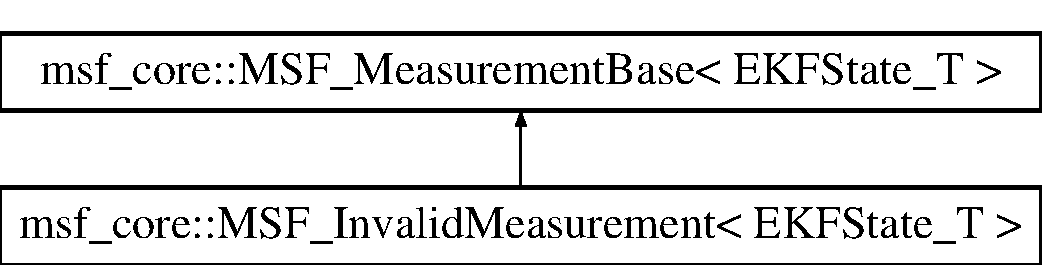
\includegraphics[height=2.000000cm]{classmsf__core_1_1MSF__InvalidMeasurement}
\end{center}
\end{figure}
\subsection*{Public Member Functions}
\begin{DoxyCompactItemize}
\item 
virtual void \hyperlink{classmsf__core_1_1MSF__InvalidMeasurement_a47d514cedc4596c60d0f0949d61200cf}{apply} (shared\-\_\-ptr$<$ E\-K\-F\-State\-\_\-\-T $>$ \hyperlink{msf__macros_8h_a2d2af1048de7b1510994ffd3bc32aacc}{U\-N\-U\-S\-E\-D\-P\-A\-R\-A\-M}(state\-With\-Covariance), \hyperlink{classmsf__core_1_1MSF__Core}{M\-S\-F\-\_\-\-Core}$<$ E\-K\-F\-State\-\_\-\-T $>$ \&\hyperlink{msf__macros_8h_a2d2af1048de7b1510994ffd3bc32aacc}{U\-N\-U\-S\-E\-D\-P\-A\-R\-A\-M}(core))
\item 
virtual std\-::string \hyperlink{classmsf__core_1_1MSF__InvalidMeasurement_abe3df54c608c49a3a26905b5d953713a}{type} ()
\item 
\hyperlink{classmsf__core_1_1MSF__InvalidMeasurement_a9de779048641efba62e57011cb54f060}{M\-S\-F\-\_\-\-Invalid\-Measurement} ()
\item 
virtual \hyperlink{classmsf__core_1_1MSF__InvalidMeasurement_aad62066f23c196f38607f66278dd0eac}{$\sim$\-M\-S\-F\-\_\-\-Invalid\-Measurement} ()
\end{DoxyCompactItemize}
\subsection*{Public Attributes}
\begin{DoxyCompactItemize}
\item 
\hyperlink{classmsf__core_1_1MSF__InvalidMeasurement_aa86e5b98f45256afded1bf30391dcce2}{E\-I\-G\-E\-N\-\_\-\-M\-A\-K\-E\-\_\-\-A\-L\-I\-G\-N\-E\-D\-\_\-\-O\-P\-E\-R\-A\-T\-O\-R\-\_\-\-N\-E\-W}
\end{DoxyCompactItemize}
\subsection*{Additional Inherited Members}


\subsection{Constructor \& Destructor Documentation}
\hypertarget{classmsf__core_1_1MSF__InvalidMeasurement_a9de779048641efba62e57011cb54f060}{\index{msf\-\_\-core\-::\-M\-S\-F\-\_\-\-Invalid\-Measurement@{msf\-\_\-core\-::\-M\-S\-F\-\_\-\-Invalid\-Measurement}!M\-S\-F\-\_\-\-Invalid\-Measurement@{M\-S\-F\-\_\-\-Invalid\-Measurement}}
\index{M\-S\-F\-\_\-\-Invalid\-Measurement@{M\-S\-F\-\_\-\-Invalid\-Measurement}!msf_core::MSF_InvalidMeasurement@{msf\-\_\-core\-::\-M\-S\-F\-\_\-\-Invalid\-Measurement}}
\subsubsection[{M\-S\-F\-\_\-\-Invalid\-Measurement}]{\setlength{\rightskip}{0pt plus 5cm}template$<$typename E\-K\-F\-State\-\_\-\-T $>$ {\bf msf\-\_\-core\-::\-M\-S\-F\-\_\-\-Invalid\-Measurement}$<$ E\-K\-F\-State\-\_\-\-T $>$\-::{\bf M\-S\-F\-\_\-\-Invalid\-Measurement} (
\begin{DoxyParamCaption}
{}
\end{DoxyParamCaption}
)\hspace{0.3cm}{\ttfamily [inline]}}}\label{classmsf__core_1_1MSF__InvalidMeasurement_a9de779048641efba62e57011cb54f060}
\hypertarget{classmsf__core_1_1MSF__InvalidMeasurement_aad62066f23c196f38607f66278dd0eac}{\index{msf\-\_\-core\-::\-M\-S\-F\-\_\-\-Invalid\-Measurement@{msf\-\_\-core\-::\-M\-S\-F\-\_\-\-Invalid\-Measurement}!$\sim$\-M\-S\-F\-\_\-\-Invalid\-Measurement@{$\sim$\-M\-S\-F\-\_\-\-Invalid\-Measurement}}
\index{$\sim$\-M\-S\-F\-\_\-\-Invalid\-Measurement@{$\sim$\-M\-S\-F\-\_\-\-Invalid\-Measurement}!msf_core::MSF_InvalidMeasurement@{msf\-\_\-core\-::\-M\-S\-F\-\_\-\-Invalid\-Measurement}}
\subsubsection[{$\sim$\-M\-S\-F\-\_\-\-Invalid\-Measurement}]{\setlength{\rightskip}{0pt plus 5cm}template$<$typename E\-K\-F\-State\-\_\-\-T $>$ virtual {\bf msf\-\_\-core\-::\-M\-S\-F\-\_\-\-Invalid\-Measurement}$<$ E\-K\-F\-State\-\_\-\-T $>$\-::$\sim${\bf M\-S\-F\-\_\-\-Invalid\-Measurement} (
\begin{DoxyParamCaption}
{}
\end{DoxyParamCaption}
)\hspace{0.3cm}{\ttfamily [inline]}, {\ttfamily [virtual]}}}\label{classmsf__core_1_1MSF__InvalidMeasurement_aad62066f23c196f38607f66278dd0eac}


\subsection{Member Function Documentation}
\hypertarget{classmsf__core_1_1MSF__InvalidMeasurement_a47d514cedc4596c60d0f0949d61200cf}{\index{msf\-\_\-core\-::\-M\-S\-F\-\_\-\-Invalid\-Measurement@{msf\-\_\-core\-::\-M\-S\-F\-\_\-\-Invalid\-Measurement}!apply@{apply}}
\index{apply@{apply}!msf_core::MSF_InvalidMeasurement@{msf\-\_\-core\-::\-M\-S\-F\-\_\-\-Invalid\-Measurement}}
\subsubsection[{apply}]{\setlength{\rightskip}{0pt plus 5cm}template$<$typename E\-K\-F\-State\-\_\-\-T $>$ virtual void {\bf msf\-\_\-core\-::\-M\-S\-F\-\_\-\-Invalid\-Measurement}$<$ E\-K\-F\-State\-\_\-\-T $>$\-::apply (
\begin{DoxyParamCaption}
\item[{shared\-\_\-ptr$<$ E\-K\-F\-State\-\_\-\-T $>$ }]{U\-N\-U\-S\-E\-D\-P\-A\-R\-A\-Mstate\-With\-Covariance, }
\item[{{\bf M\-S\-F\-\_\-\-Core}$<$ E\-K\-F\-State\-\_\-\-T $>$ \&}]{U\-N\-U\-S\-E\-D\-P\-A\-R\-A\-Mcore}
\end{DoxyParamCaption}
)\hspace{0.3cm}{\ttfamily [inline]}, {\ttfamily [virtual]}}}\label{classmsf__core_1_1MSF__InvalidMeasurement_a47d514cedc4596c60d0f0949d61200cf}
\hypertarget{classmsf__core_1_1MSF__InvalidMeasurement_abe3df54c608c49a3a26905b5d953713a}{\index{msf\-\_\-core\-::\-M\-S\-F\-\_\-\-Invalid\-Measurement@{msf\-\_\-core\-::\-M\-S\-F\-\_\-\-Invalid\-Measurement}!type@{type}}
\index{type@{type}!msf_core::MSF_InvalidMeasurement@{msf\-\_\-core\-::\-M\-S\-F\-\_\-\-Invalid\-Measurement}}
\subsubsection[{type}]{\setlength{\rightskip}{0pt plus 5cm}template$<$typename E\-K\-F\-State\-\_\-\-T $>$ virtual std\-::string {\bf msf\-\_\-core\-::\-M\-S\-F\-\_\-\-Invalid\-Measurement}$<$ E\-K\-F\-State\-\_\-\-T $>$\-::type (
\begin{DoxyParamCaption}
{}
\end{DoxyParamCaption}
)\hspace{0.3cm}{\ttfamily [inline]}, {\ttfamily [virtual]}}}\label{classmsf__core_1_1MSF__InvalidMeasurement_abe3df54c608c49a3a26905b5d953713a}


Implements \hyperlink{classmsf__core_1_1MSF__MeasurementBase_a6a711d7ed976c0aed497efc1b8fbe3e7}{msf\-\_\-core\-::\-M\-S\-F\-\_\-\-Measurement\-Base$<$ E\-K\-F\-State\-\_\-\-T $>$}.



\subsection{Member Data Documentation}
\hypertarget{classmsf__core_1_1MSF__InvalidMeasurement_aa86e5b98f45256afded1bf30391dcce2}{\index{msf\-\_\-core\-::\-M\-S\-F\-\_\-\-Invalid\-Measurement@{msf\-\_\-core\-::\-M\-S\-F\-\_\-\-Invalid\-Measurement}!E\-I\-G\-E\-N\-\_\-\-M\-A\-K\-E\-\_\-\-A\-L\-I\-G\-N\-E\-D\-\_\-\-O\-P\-E\-R\-A\-T\-O\-R\-\_\-\-N\-E\-W@{E\-I\-G\-E\-N\-\_\-\-M\-A\-K\-E\-\_\-\-A\-L\-I\-G\-N\-E\-D\-\_\-\-O\-P\-E\-R\-A\-T\-O\-R\-\_\-\-N\-E\-W}}
\index{E\-I\-G\-E\-N\-\_\-\-M\-A\-K\-E\-\_\-\-A\-L\-I\-G\-N\-E\-D\-\_\-\-O\-P\-E\-R\-A\-T\-O\-R\-\_\-\-N\-E\-W@{E\-I\-G\-E\-N\-\_\-\-M\-A\-K\-E\-\_\-\-A\-L\-I\-G\-N\-E\-D\-\_\-\-O\-P\-E\-R\-A\-T\-O\-R\-\_\-\-N\-E\-W}!msf_core::MSF_InvalidMeasurement@{msf\-\_\-core\-::\-M\-S\-F\-\_\-\-Invalid\-Measurement}}
\subsubsection[{E\-I\-G\-E\-N\-\_\-\-M\-A\-K\-E\-\_\-\-A\-L\-I\-G\-N\-E\-D\-\_\-\-O\-P\-E\-R\-A\-T\-O\-R\-\_\-\-N\-E\-W}]{\setlength{\rightskip}{0pt plus 5cm}template$<$typename E\-K\-F\-State\-\_\-\-T $>$ {\bf msf\-\_\-core\-::\-M\-S\-F\-\_\-\-Invalid\-Measurement}$<$ E\-K\-F\-State\-\_\-\-T $>$\-::E\-I\-G\-E\-N\-\_\-\-M\-A\-K\-E\-\_\-\-A\-L\-I\-G\-N\-E\-D\-\_\-\-O\-P\-E\-R\-A\-T\-O\-R\-\_\-\-N\-E\-W}}\label{classmsf__core_1_1MSF__InvalidMeasurement_aa86e5b98f45256afded1bf30391dcce2}


The documentation for this class was generated from the following file\-:\begin{DoxyCompactItemize}
\item 
msf\-\_\-core/include/msf\-\_\-core/\hyperlink{msf__measurement_8h}{msf\-\_\-measurement.\-h}\end{DoxyCompactItemize}

\hypertarget{classmsf__core_1_1MSF__Measurement}{\section{msf\-\_\-core\-:\-:M\-S\-F\-\_\-\-Measurement$<$ T, R\-M\-A\-T\-\_\-\-T, E\-K\-F\-State\-\_\-\-T $>$ Class Template Reference}
\label{classmsf__core_1_1MSF__Measurement}\index{msf\-\_\-core\-::\-M\-S\-F\-\_\-\-Measurement$<$ T, R\-M\-A\-T\-\_\-\-T, E\-K\-F\-State\-\_\-\-T $>$@{msf\-\_\-core\-::\-M\-S\-F\-\_\-\-Measurement$<$ T, R\-M\-A\-T\-\_\-\-T, E\-K\-F\-State\-\_\-\-T $>$}}
}


The class for sensor based measurements which we want to apply to a state in the update routine of the E\-K\-F. This calls the apply correction method of the E\-K\-F core.  




{\ttfamily \#include $<$msf\-\_\-measurement.\-h$>$}

Inheritance diagram for msf\-\_\-core\-:\-:M\-S\-F\-\_\-\-Measurement$<$ T, R\-M\-A\-T\-\_\-\-T, E\-K\-F\-State\-\_\-\-T $>$\-:\begin{figure}[H]
\begin{center}
\leavevmode
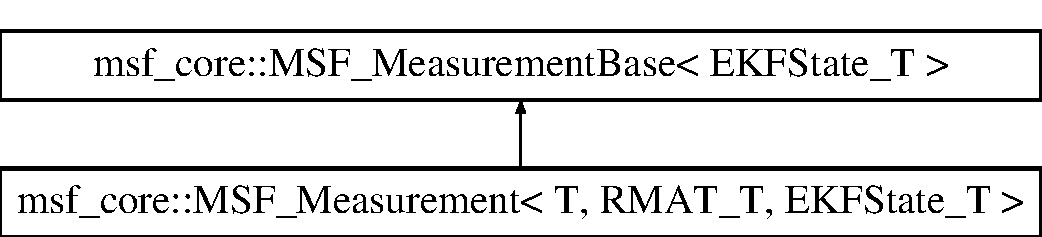
\includegraphics[height=2.000000cm]{classmsf__core_1_1MSF__Measurement}
\end{center}
\end{figure}
\subsection*{Public Types}
\begin{DoxyCompactItemize}
\item 
\hypertarget{classmsf__core_1_1MSF__Measurement_ab102d2c17bef09be28cb1403017992b6}{typedef T {\bfseries Measurement\-\_\-type}}\label{classmsf__core_1_1MSF__Measurement_ab102d2c17bef09be28cb1403017992b6}

\item 
\hypertarget{classmsf__core_1_1MSF__Measurement_afa4f826dadcfd129a50330f078a8dbf8}{typedef boost\-::shared\-\_\-ptr$<$ T \\*
const  $>$ {\bfseries Measurement\-\_\-ptr}}\label{classmsf__core_1_1MSF__Measurement_afa4f826dadcfd129a50330f078a8dbf8}

\end{DoxyCompactItemize}
\subsection*{Public Member Functions}
\begin{DoxyCompactItemize}
\item 
\hypertarget{classmsf__core_1_1MSF__Measurement_a33143412cbcabec0c16e1c6ad82641d0}{{\bfseries M\-S\-F\-\_\-\-Measurement} (bool is\-Absolute\-Measurement, int sensor\-I\-D)}\label{classmsf__core_1_1MSF__Measurement_a33143412cbcabec0c16e1c6ad82641d0}

\item 
\hypertarget{classmsf__core_1_1MSF__Measurement_a345b17105929ac6c70a0a5d21e281a5c}{void {\bfseries make\-From\-Sensor\-Reading} (const boost\-::shared\-\_\-ptr$<$ T const  $>$ reading, double timestamp)}\label{classmsf__core_1_1MSF__Measurement_a345b17105929ac6c70a0a5d21e281a5c}

\end{DoxyCompactItemize}
\subsection*{Public Attributes}
\begin{DoxyCompactItemize}
\item 
\hypertarget{classmsf__core_1_1MSF__Measurement_a481fa3230f73f28a8489223311c3033f}{{\bfseries E\-I\-G\-E\-N\-\_\-\-M\-A\-K\-E\-\_\-\-A\-L\-I\-G\-N\-E\-D\-\_\-\-O\-P\-E\-R\-A\-T\-O\-R\-\_\-\-N\-E\-W}}\label{classmsf__core_1_1MSF__Measurement_a481fa3230f73f28a8489223311c3033f}

\end{DoxyCompactItemize}
\subsection*{Protected Attributes}
\begin{DoxyCompactItemize}
\item 
\hypertarget{classmsf__core_1_1MSF__Measurement_a20fcacb533df8a1e6ae4fad4a3eb06ec}{R\-M\-A\-T\-\_\-\-T {\bfseries R\-\_\-}}\label{classmsf__core_1_1MSF__Measurement_a20fcacb533df8a1e6ae4fad4a3eb06ec}

\end{DoxyCompactItemize}
\subsection*{Additional Inherited Members}


\subsection{Detailed Description}
\subsubsection*{template$<$typename T, typename R\-M\-A\-T\-\_\-\-T, typename E\-K\-F\-State\-\_\-\-T$>$class msf\-\_\-core\-::\-M\-S\-F\-\_\-\-Measurement$<$ T, R\-M\-A\-T\-\_\-\-T, E\-K\-F\-State\-\_\-\-T $>$}

The class for sensor based measurements which we want to apply to a state in the update routine of the E\-K\-F. This calls the apply correction method of the E\-K\-F core. 

\begin{DoxyNote}{Note}
Provides an abstract N\-V\-I to create measurements from sensor readings. 
\end{DoxyNote}


The documentation for this class was generated from the following file\-:\begin{DoxyCompactItemize}
\item 
msf\-\_\-core/include/msf\-\_\-core/msf\-\_\-measurement.\-h\end{DoxyCompactItemize}

\hypertarget{classmsf__core_1_1MSF__MeasurementBase}{\section{msf\-\_\-core\-:\-:M\-S\-F\-\_\-\-Measurement\-Base$<$ E\-K\-F\-State\-\_\-\-T $>$ Class Template Reference}
\label{classmsf__core_1_1MSF__MeasurementBase}\index{msf\-\_\-core\-::\-M\-S\-F\-\_\-\-Measurement\-Base$<$ E\-K\-F\-State\-\_\-\-T $>$@{msf\-\_\-core\-::\-M\-S\-F\-\_\-\-Measurement\-Base$<$ E\-K\-F\-State\-\_\-\-T $>$}}
}


The base class for all measurement types. These are the objects provided to the E\-K\-F core to be applied in correct order to the states.  




{\ttfamily \#include $<$msf\-\_\-measurement.\-h$>$}

Inheritance diagram for msf\-\_\-core\-:\-:M\-S\-F\-\_\-\-Measurement\-Base$<$ E\-K\-F\-State\-\_\-\-T $>$\-:\begin{figure}[H]
\begin{center}
\leavevmode
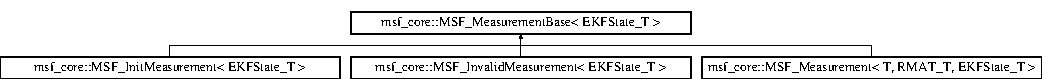
\includegraphics[height=1.060606cm]{classmsf__core_1_1MSF__MeasurementBase}
\end{center}
\end{figure}
\subsection*{Public Member Functions}
\begin{DoxyCompactItemize}
\item 
\hypertarget{classmsf__core_1_1MSF__MeasurementBase_a415d8c321cebf22510cce29f69a3b22f}{E\-I\-G\-E\-N\-\_\-\-M\-A\-K\-E\-\_\-\-A\-L\-I\-G\-N\-E\-D\-\_\-\-O\-P\-E\-R\-A\-T\-O\-R\-\_\-\-N\-E\-W {\bfseries M\-S\-F\-\_\-\-Measurement\-Base} (bool isabsolute\-Measurement, int sensor\-I\-D)}\label{classmsf__core_1_1MSF__MeasurementBase_a415d8c321cebf22510cce29f69a3b22f}

\item 
\hypertarget{classmsf__core_1_1MSF__MeasurementBase_ac1c4001e0c61b7cd2b551c0adeae7109}{virtual void \hyperlink{classmsf__core_1_1MSF__MeasurementBase_ac1c4001e0c61b7cd2b551c0adeae7109}{apply} (shared\-\_\-ptr$<$ E\-K\-F\-State\-\_\-\-T $>$ state\-With\-Covariance, \hyperlink{classmsf__core_1_1MSF__Core}{M\-S\-F\-\_\-\-Core}$<$ E\-K\-F\-State\-\_\-\-T $>$ \&core)=0}\label{classmsf__core_1_1MSF__MeasurementBase_ac1c4001e0c61b7cd2b551c0adeae7109}

\begin{DoxyCompactList}\small\item\em The method called by the msf\-\_\-core to apply the measurement represented by this object. \end{DoxyCompactList}\item 
\hypertarget{classmsf__core_1_1MSF__MeasurementBase_a6a711d7ed976c0aed497efc1b8fbe3e7}{virtual std\-::string {\bfseries type} ()=0}\label{classmsf__core_1_1MSF__MeasurementBase_a6a711d7ed976c0aed497efc1b8fbe3e7}

\end{DoxyCompactItemize}
\subsection*{Public Attributes}
\begin{DoxyCompactItemize}
\item 
\hypertarget{classmsf__core_1_1MSF__MeasurementBase_afad7c30029f47cea027415c04301dc48}{int {\bfseries sensor\-I\-D\-\_\-}}\label{classmsf__core_1_1MSF__MeasurementBase_afad7c30029f47cea027415c04301dc48}

\item 
\hypertarget{classmsf__core_1_1MSF__MeasurementBase_ad1ea7c4d392ecd3d894280283c04757a}{bool {\bfseries isabsolute\-\_\-}}\label{classmsf__core_1_1MSF__MeasurementBase_ad1ea7c4d392ecd3d894280283c04757a}

\item 
\hypertarget{classmsf__core_1_1MSF__MeasurementBase_a48b55b129f13afbed86db1b0543562db}{double \hyperlink{classmsf__core_1_1MSF__MeasurementBase_a48b55b129f13afbed86db1b0543562db}{time}}\label{classmsf__core_1_1MSF__MeasurementBase_a48b55b129f13afbed86db1b0543562db}

\begin{DoxyCompactList}\small\item\em The time\-\_\- this measurement was taken. \end{DoxyCompactList}\end{DoxyCompactItemize}
\subsection*{Protected Member Functions}
\begin{DoxyCompactItemize}
\item 
{\footnotesize template$<$class H\-\_\-type , class Res\-\_\-type , class R\-\_\-type $>$ }\\void \hyperlink{classmsf__core_1_1MSF__MeasurementBase_a569c0772641a11d707349aab9dc0da7e}{calculate\-And\-Apply\-Correction} (shared\-\_\-ptr$<$ E\-K\-F\-State\-\_\-\-T $>$ state, \hyperlink{classmsf__core_1_1MSF__Core}{M\-S\-F\-\_\-\-Core}$<$ E\-K\-F\-State\-\_\-\-T $>$ \&core, const Eigen\-::\-Matrix\-Base$<$ H\-\_\-type $>$ \&H, const Eigen\-::\-Matrix\-Base$<$ Res\-\_\-type $>$ \&residual, const Eigen\-::\-Matrix\-Base$<$ R\-\_\-type $>$ \&R)
\item 
void \hyperlink{classmsf__core_1_1MSF__MeasurementBase_ade8ddcc9ef64571451560079381ecc64}{calculate\-And\-Apply\-Correction} (shared\-\_\-ptr$<$ E\-K\-F\-State\-\_\-\-T $>$ state, \hyperlink{classmsf__core_1_1MSF__Core}{M\-S\-F\-\_\-\-Core}$<$ E\-K\-F\-State\-\_\-\-T $>$ \&core, const Eigen\-::\-Matrix\-Xd \&H, const Eigen\-::\-Matrix\-Xd \&residual, const Eigen\-::\-Matrix\-Xd \&R)
\item 
{\footnotesize template$<$class H\-\_\-type , class Res\-\_\-type , class R\-\_\-type $>$ }\\void \hyperlink{classmsf__core_1_1MSF__MeasurementBase_a5b9db1020711ae6b5ba4e877dd03fa42}{calculate\-And\-Apply\-Correction\-Relative} (shared\-\_\-ptr$<$ E\-K\-F\-State\-\_\-\-T $>$ state\-\_\-old, shared\-\_\-ptr$<$ E\-K\-F\-State\-\_\-\-T $>$ state\-\_\-new, \hyperlink{classmsf__core_1_1MSF__Core}{M\-S\-F\-\_\-\-Core}$<$ E\-K\-F\-State\-\_\-\-T $>$ \&core, const Eigen\-::\-Matrix\-Base$<$ H\-\_\-type $>$ \&H\-\_\-old, const Eigen\-::\-Matrix\-Base$<$ H\-\_\-type $>$ \&H\-\_\-new, const Eigen\-::\-Matrix\-Base$<$ Res\-\_\-type $>$ \&residual, const Eigen\-::\-Matrix\-Base$<$ R\-\_\-type $>$ \&R)
\end{DoxyCompactItemize}


\subsection{Detailed Description}
\subsubsection*{template$<$typename E\-K\-F\-State\-\_\-\-T$>$class msf\-\_\-core\-::\-M\-S\-F\-\_\-\-Measurement\-Base$<$ E\-K\-F\-State\-\_\-\-T $>$}

The base class for all measurement types. These are the objects provided to the E\-K\-F core to be applied in correct order to the states. 

\subsection{Member Function Documentation}
\hypertarget{classmsf__core_1_1MSF__MeasurementBase_a569c0772641a11d707349aab9dc0da7e}{\index{msf\-\_\-core\-::\-M\-S\-F\-\_\-\-Measurement\-Base@{msf\-\_\-core\-::\-M\-S\-F\-\_\-\-Measurement\-Base}!calculate\-And\-Apply\-Correction@{calculate\-And\-Apply\-Correction}}
\index{calculate\-And\-Apply\-Correction@{calculate\-And\-Apply\-Correction}!msf_core::MSF_MeasurementBase@{msf\-\_\-core\-::\-M\-S\-F\-\_\-\-Measurement\-Base}}
\subsubsection[{calculate\-And\-Apply\-Correction}]{\setlength{\rightskip}{0pt plus 5cm}template$<$typename E\-K\-F\-State\-\_\-\-T $>$ template$<$class H\-\_\-type , class Res\-\_\-type , class R\-\_\-type $>$ void {\bf msf\-\_\-core\-::\-M\-S\-F\-\_\-\-Measurement\-Base}$<$ E\-K\-F\-State\-\_\-\-T $>$\-::calculate\-And\-Apply\-Correction (
\begin{DoxyParamCaption}
\item[{shared\-\_\-ptr$<$ E\-K\-F\-State\-\_\-\-T $>$}]{state, }
\item[{{\bf M\-S\-F\-\_\-\-Core}$<$ E\-K\-F\-State\-\_\-\-T $>$ \&}]{core, }
\item[{const Eigen\-::\-Matrix\-Base$<$ H\-\_\-type $>$ \&}]{H, }
\item[{const Eigen\-::\-Matrix\-Base$<$ Res\-\_\-type $>$ \&}]{residual, }
\item[{const Eigen\-::\-Matrix\-Base$<$ R\-\_\-type $>$ \&}]{R}
\end{DoxyParamCaption}
)\hspace{0.3cm}{\ttfamily [protected]}}}\label{classmsf__core_1_1MSF__MeasurementBase_a569c0772641a11d707349aab9dc0da7e}
Main update routine called by a given sensor, will apply the measurement to the state inside the core. Correction from E\-K\-F update. \hypertarget{classmsf__core_1_1MSF__MeasurementBase_ade8ddcc9ef64571451560079381ecc64}{\index{msf\-\_\-core\-::\-M\-S\-F\-\_\-\-Measurement\-Base@{msf\-\_\-core\-::\-M\-S\-F\-\_\-\-Measurement\-Base}!calculate\-And\-Apply\-Correction@{calculate\-And\-Apply\-Correction}}
\index{calculate\-And\-Apply\-Correction@{calculate\-And\-Apply\-Correction}!msf_core::MSF_MeasurementBase@{msf\-\_\-core\-::\-M\-S\-F\-\_\-\-Measurement\-Base}}
\subsubsection[{calculate\-And\-Apply\-Correction}]{\setlength{\rightskip}{0pt plus 5cm}template$<$typename E\-K\-F\-State\-\_\-\-T $>$ void {\bf msf\-\_\-core\-::\-M\-S\-F\-\_\-\-Measurement\-Base}$<$ E\-K\-F\-State\-\_\-\-T $>$\-::calculate\-And\-Apply\-Correction (
\begin{DoxyParamCaption}
\item[{shared\-\_\-ptr$<$ E\-K\-F\-State\-\_\-\-T $>$}]{state, }
\item[{{\bf M\-S\-F\-\_\-\-Core}$<$ E\-K\-F\-State\-\_\-\-T $>$ \&}]{core, }
\item[{const Eigen\-::\-Matrix\-Xd \&}]{H, }
\item[{const Eigen\-::\-Matrix\-Xd \&}]{residual, }
\item[{const Eigen\-::\-Matrix\-Xd \&}]{R}
\end{DoxyParamCaption}
)\hspace{0.3cm}{\ttfamily [protected]}}}\label{classmsf__core_1_1MSF__MeasurementBase_ade8ddcc9ef64571451560079381ecc64}
Correction from E\-K\-F update. \hypertarget{classmsf__core_1_1MSF__MeasurementBase_a5b9db1020711ae6b5ba4e877dd03fa42}{\index{msf\-\_\-core\-::\-M\-S\-F\-\_\-\-Measurement\-Base@{msf\-\_\-core\-::\-M\-S\-F\-\_\-\-Measurement\-Base}!calculate\-And\-Apply\-Correction\-Relative@{calculate\-And\-Apply\-Correction\-Relative}}
\index{calculate\-And\-Apply\-Correction\-Relative@{calculate\-And\-Apply\-Correction\-Relative}!msf_core::MSF_MeasurementBase@{msf\-\_\-core\-::\-M\-S\-F\-\_\-\-Measurement\-Base}}
\subsubsection[{calculate\-And\-Apply\-Correction\-Relative}]{\setlength{\rightskip}{0pt plus 5cm}template$<$typename E\-K\-F\-State\-\_\-\-T $>$ template$<$class H\-\_\-type , class Res\-\_\-type , class R\-\_\-type $>$ void {\bf msf\-\_\-core\-::\-M\-S\-F\-\_\-\-Measurement\-Base}$<$ E\-K\-F\-State\-\_\-\-T $>$\-::calculate\-And\-Apply\-Correction\-Relative (
\begin{DoxyParamCaption}
\item[{shared\-\_\-ptr$<$ E\-K\-F\-State\-\_\-\-T $>$}]{state\-\_\-old, }
\item[{shared\-\_\-ptr$<$ E\-K\-F\-State\-\_\-\-T $>$}]{state\-\_\-new, }
\item[{{\bf M\-S\-F\-\_\-\-Core}$<$ E\-K\-F\-State\-\_\-\-T $>$ \&}]{core, }
\item[{const Eigen\-::\-Matrix\-Base$<$ H\-\_\-type $>$ \&}]{H\-\_\-old, }
\item[{const Eigen\-::\-Matrix\-Base$<$ H\-\_\-type $>$ \&}]{H\-\_\-new, }
\item[{const Eigen\-::\-Matrix\-Base$<$ Res\-\_\-type $>$ \&}]{residual, }
\item[{const Eigen\-::\-Matrix\-Base$<$ R\-\_\-type $>$ \&}]{R}
\end{DoxyParamCaption}
)\hspace{0.3cm}{\ttfamily [protected]}}}\label{classmsf__core_1_1MSF__MeasurementBase_a5b9db1020711ae6b5ba4e877dd03fa42}
Correction from E\-K\-F update. 

The documentation for this class was generated from the following files\-:\begin{DoxyCompactItemize}
\item 
msf\-\_\-core/include/msf\-\_\-core/msf\-\_\-measurement.\-h\item 
msf\-\_\-core/include/msf\-\_\-core/implementation/msf\-\_\-measurement.\-hpp\end{DoxyCompactItemize}

\hypertarget{classmsf__core_1_1MSF__SensorManager}{\section{msf\-\_\-core\-:\-:M\-S\-F\-\_\-\-Sensor\-Manager$<$ E\-K\-F\-State\-\_\-\-T $>$ Class Template Reference}
\label{classmsf__core_1_1MSF__SensorManager}\index{msf\-\_\-core\-::\-M\-S\-F\-\_\-\-Sensor\-Manager$<$ E\-K\-F\-State\-\_\-\-T $>$@{msf\-\_\-core\-::\-M\-S\-F\-\_\-\-Sensor\-Manager$<$ E\-K\-F\-State\-\_\-\-T $>$}}
}


A manager for a given sensor set. Handlers for individual sensors (camera/vicon etc.) are registered with this class as handlers of particular sensors. This class also owns the E\-K\-F core instance and handles the initialization of the filter.  




{\ttfamily \#include $<$msf\-\_\-sensormanager.\-h$>$}

Inheritance diagram for msf\-\_\-core\-:\-:M\-S\-F\-\_\-\-Sensor\-Manager$<$ E\-K\-F\-State\-\_\-\-T $>$\-:\begin{figure}[H]
\begin{center}
\leavevmode
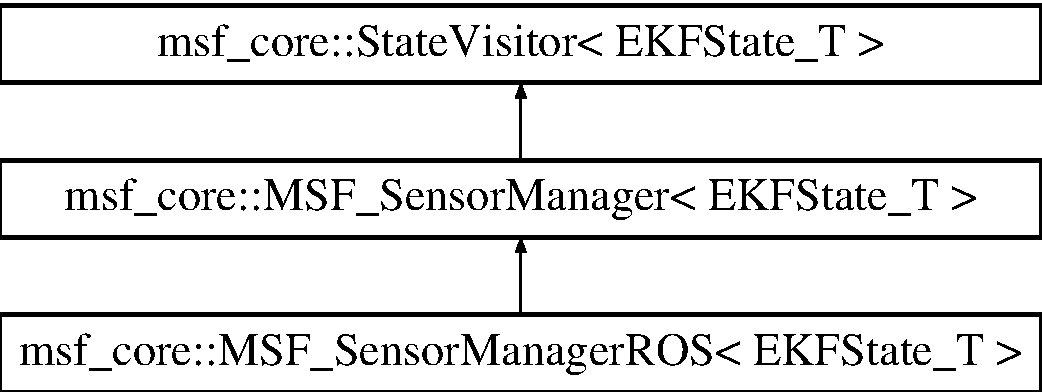
\includegraphics[height=3.000000cm]{classmsf__core_1_1MSF__SensorManager}
\end{center}
\end{figure}
\subsection*{Public Member Functions}
\begin{DoxyCompactItemize}
\item 
\hypertarget{classmsf__core_1_1MSF__SensorManager_a50c42d9ed661147254d94c603b09691f}{bool {\bfseries data\-\_\-playback} ()}\label{classmsf__core_1_1MSF__SensorManager_a50c42d9ed661147254d94c603b09691f}

\item 
\hypertarget{classmsf__core_1_1MSF__SensorManager_a106ff842a5280f1799505a7203ad2c08}{void {\bfseries add\-Handler} (shared\-\_\-ptr$<$ \hyperlink{classmsf__core_1_1SensorHandler}{Sensor\-Handler}$<$ E\-K\-F\-State\-\_\-\-T $>$ $>$ handler)}\label{classmsf__core_1_1MSF__SensorManager_a106ff842a5280f1799505a7203ad2c08}

\item 
\hypertarget{classmsf__core_1_1MSF__SensorManager_a170802bb97dfc3afb931fd1d7779e3ac}{virtual void {\bfseries init} (double scale) const =0}\label{classmsf__core_1_1MSF__SensorManager_a170802bb97dfc3afb931fd1d7779e3ac}

\item 
\hypertarget{classmsf__core_1_1MSF__SensorManager_a326567c3181be5b0854b294431aa69ff}{virtual void {\bfseries init\-State} (E\-K\-F\-State\-\_\-\-T \&state) const =0}\label{classmsf__core_1_1MSF__SensorManager_a326567c3181be5b0854b294431aa69ff}

\item 
\hypertarget{classmsf__core_1_1MSF__SensorManager_afc9c8189b990db3c00df9bc239ff14e8}{virtual void {\bfseries calculate\-Q\-Auxiliary\-States} (E\-K\-F\-State\-\_\-\-T \&U\-N\-U\-S\-E\-D\-P\-A\-R\-A\-M(state), double U\-N\-U\-S\-E\-D\-P\-A\-R\-A\-M(dt)) const =0}\label{classmsf__core_1_1MSF__SensorManager_afc9c8189b990db3c00df9bc239ff14e8}

\item 
\hypertarget{classmsf__core_1_1MSF__SensorManager_a586c046dc1ffbe4f236c7c4413a8dc82}{virtual void {\bfseries set\-P} (Eigen\-::\-Matrix$<$ double, E\-K\-F\-State\-\_\-\-T\-::n\-Error\-States\-At\-Compile\-Time, E\-K\-F\-State\-\_\-\-T\-::n\-Error\-States\-At\-Compile\-Time $>$ \&P) const =0}\label{classmsf__core_1_1MSF__SensorManager_a586c046dc1ffbe4f236c7c4413a8dc82}

\item 
\hypertarget{classmsf__core_1_1MSF__SensorManager_a9f69dacac4e600a524691dd4c17f94a0}{virtual void {\bfseries augment\-Correction\-Vector} (Eigen\-::\-Matrix$<$ double, E\-K\-F\-State\-\_\-\-T\-::n\-Error\-States\-At\-Compile\-Time, 1 $>$ \&U\-N\-U\-S\-E\-D\-P\-A\-R\-A\-M(correction)) const =0}\label{classmsf__core_1_1MSF__SensorManager_a9f69dacac4e600a524691dd4c17f94a0}

\item 
\hypertarget{classmsf__core_1_1MSF__SensorManager_ae605f79877bbdd7ec297d5fe375f4c92}{virtual void {\bfseries sanity\-Check\-Correction} (E\-K\-F\-State\-\_\-\-T \&U\-N\-U\-S\-E\-D\-P\-A\-R\-A\-M(delaystate), const E\-K\-F\-State\-\_\-\-T \&U\-N\-U\-S\-E\-D\-P\-A\-R\-A\-M(buffstate), Eigen\-::\-Matrix$<$ double, E\-K\-F\-State\-\_\-\-T\-::n\-Error\-States\-At\-Compile\-Time, 1 $>$ \&U\-N\-U\-S\-E\-D\-P\-A\-R\-A\-M(correction)) const =0}\label{classmsf__core_1_1MSF__SensorManager_ae605f79877bbdd7ec297d5fe375f4c92}

\item 
\hypertarget{classmsf__core_1_1MSF__SensorManager_a5eb7188dea0d2aa231732199fd06b988}{virtual bool {\bfseries get\-Param\-\_\-fixed\-\_\-bias} () const =0}\label{classmsf__core_1_1MSF__SensorManager_a5eb7188dea0d2aa231732199fd06b988}

\item 
\hypertarget{classmsf__core_1_1MSF__SensorManager_a647bebf2feecd2929f58d6b4c8b3b319}{virtual double {\bfseries get\-Param\-\_\-noise\-\_\-acc} () const =0}\label{classmsf__core_1_1MSF__SensorManager_a647bebf2feecd2929f58d6b4c8b3b319}

\item 
\hypertarget{classmsf__core_1_1MSF__SensorManager_a7e7342acff24a4b5c5817903b2c8dfda}{virtual double {\bfseries get\-Param\-\_\-noise\-\_\-accbias} () const =0}\label{classmsf__core_1_1MSF__SensorManager_a7e7342acff24a4b5c5817903b2c8dfda}

\item 
\hypertarget{classmsf__core_1_1MSF__SensorManager_ae7b3b5a203fe118961ecdf28b49bfaa9}{virtual double {\bfseries get\-Param\-\_\-noise\-\_\-gyr} () const =0}\label{classmsf__core_1_1MSF__SensorManager_ae7b3b5a203fe118961ecdf28b49bfaa9}

\item 
\hypertarget{classmsf__core_1_1MSF__SensorManager_a8a5c694d3c6e5bd5bf4724269613bcb6}{virtual double {\bfseries get\-Param\-\_\-noise\-\_\-gyrbias} () const =0}\label{classmsf__core_1_1MSF__SensorManager_a8a5c694d3c6e5bd5bf4724269613bcb6}

\item 
\hypertarget{classmsf__core_1_1MSF__SensorManager_ab4498922d3d876ed9c4c5eeb7e090529}{virtual double {\bfseries get\-Param\-\_\-fuzzythres} () const =0}\label{classmsf__core_1_1MSF__SensorManager_ab4498922d3d876ed9c4c5eeb7e090529}

\item 
virtual void \hyperlink{classmsf__core_1_1MSF__SensorManager_ad851fff1bceaeb6696ef79a4792a317a}{publish\-State\-Initial} (const shared\-\_\-ptr$<$ E\-K\-F\-State\-\_\-\-T $>$ \&state) const =0
\item 
\hypertarget{classmsf__core_1_1MSF__SensorManager_a431f5b517c39fd9b2168857ae9513f8b}{virtual void {\bfseries publish\-State\-After\-Propagation} (const shared\-\_\-ptr$<$ E\-K\-F\-State\-\_\-\-T $>$ \&state) const =0}\label{classmsf__core_1_1MSF__SensorManager_a431f5b517c39fd9b2168857ae9513f8b}

\item 
\hypertarget{classmsf__core_1_1MSF__SensorManager_abbce1dfe246d7c58ec94529d70c862e5}{virtual void {\bfseries publish\-State\-After\-Update} (const shared\-\_\-ptr$<$ E\-K\-F\-State\-\_\-\-T $>$ \&state) const =0}\label{classmsf__core_1_1MSF__SensorManager_abbce1dfe246d7c58ec94529d70c862e5}

\end{DoxyCompactItemize}
\subsection*{Public Attributes}
\begin{DoxyCompactItemize}
\item 
\hypertarget{classmsf__core_1_1MSF__SensorManager_ad08942e66e76a572cd6425b79e653fd2}{E\-I\-G\-E\-N\-\_\-\-M\-A\-K\-E\-\_\-\-A\-L\-I\-G\-N\-E\-D\-\_\-\-O\-P\-E\-R\-A\-T\-O\-R\-\_\-\-N\-E\-W \\*
shared\-\_\-ptr$<$ \hyperlink{classmsf__core_1_1MSF__Core}{M\-S\-F\-\_\-\-Core}\\*
$<$ E\-K\-F\-State\-\_\-\-T $>$ $>$ \hyperlink{classmsf__core_1_1MSF__SensorManager_ad08942e66e76a572cd6425b79e653fd2}{msf\-\_\-core\-\_\-}}\label{classmsf__core_1_1MSF__SensorManager_ad08942e66e76a572cd6425b79e653fd2}

\begin{DoxyCompactList}\small\item\em The ekf core instance. \end{DoxyCompactList}\end{DoxyCompactItemize}
\subsection*{Protected Types}
\begin{DoxyCompactItemize}
\item 
\hypertarget{classmsf__core_1_1MSF__SensorManager_a4bcde5443748c5580b583f2056d4dc67}{typedef std\-::vector\\*
$<$ shared\-\_\-ptr$<$ \hyperlink{classmsf__core_1_1SensorHandler}{Sensor\-Handler}\\*
$<$ E\-K\-F\-State\-\_\-\-T $>$ $>$ $>$ {\bfseries Handlers}}\label{classmsf__core_1_1MSF__SensorManager_a4bcde5443748c5580b583f2056d4dc67}

\end{DoxyCompactItemize}
\subsection*{Protected Attributes}
\begin{DoxyCompactItemize}
\item 
\hypertarget{classmsf__core_1_1MSF__SensorManager_a7c6fe8b491f541562cbf863c452891fd}{Handlers \hyperlink{classmsf__core_1_1MSF__SensorManager_a7c6fe8b491f541562cbf863c452891fd}{handlers}}\label{classmsf__core_1_1MSF__SensorManager_a7c6fe8b491f541562cbf863c452891fd}

\begin{DoxyCompactList}\small\item\em A list of sensor handlers which provide measurements. \end{DoxyCompactList}\item 
bool \hyperlink{classmsf__core_1_1MSF__SensorManager_a49ac85275688e5588b73ed98795abe1a}{data\-\_\-playback\-\_\-}
\end{DoxyCompactItemize}


\subsection{Detailed Description}
\subsubsection*{template$<$typename E\-K\-F\-State\-\_\-\-T$>$class msf\-\_\-core\-::\-M\-S\-F\-\_\-\-Sensor\-Manager$<$ E\-K\-F\-State\-\_\-\-T $>$}

A manager for a given sensor set. Handlers for individual sensors (camera/vicon etc.) are registered with this class as handlers of particular sensors. This class also owns the E\-K\-F core instance and handles the initialization of the filter. 

\subsection{Member Function Documentation}
\hypertarget{classmsf__core_1_1MSF__SensorManager_ad851fff1bceaeb6696ef79a4792a317a}{\index{msf\-\_\-core\-::\-M\-S\-F\-\_\-\-Sensor\-Manager@{msf\-\_\-core\-::\-M\-S\-F\-\_\-\-Sensor\-Manager}!publish\-State\-Initial@{publish\-State\-Initial}}
\index{publish\-State\-Initial@{publish\-State\-Initial}!msf_core::MSF_SensorManager@{msf\-\_\-core\-::\-M\-S\-F\-\_\-\-Sensor\-Manager}}
\subsubsection[{publish\-State\-Initial}]{\setlength{\rightskip}{0pt plus 5cm}template$<$typename E\-K\-F\-State\-\_\-\-T$>$ virtual void {\bf msf\-\_\-core\-::\-M\-S\-F\-\_\-\-Sensor\-Manager}$<$ E\-K\-F\-State\-\_\-\-T $>$\-::publish\-State\-Initial (
\begin{DoxyParamCaption}
\item[{const shared\-\_\-ptr$<$ E\-K\-F\-State\-\_\-\-T $>$ \&}]{state}
\end{DoxyParamCaption}
) const\hspace{0.3cm}{\ttfamily [pure virtual]}}}\label{classmsf__core_1_1MSF__SensorManager_ad851fff1bceaeb6696ef79a4792a317a}
This functions get called by the core to publish data to external middlewares like R\-O\-S. 

Implemented in \hyperlink{structmsf__core_1_1MSF__SensorManagerROS_abde229602f1aeb393a2aad30ef413e12}{msf\-\_\-core\-::\-M\-S\-F\-\_\-\-Sensor\-Manager\-R\-O\-S$<$ E\-K\-F\-State\-\_\-\-T $>$}.



\subsection{Member Data Documentation}
\hypertarget{classmsf__core_1_1MSF__SensorManager_a49ac85275688e5588b73ed98795abe1a}{\index{msf\-\_\-core\-::\-M\-S\-F\-\_\-\-Sensor\-Manager@{msf\-\_\-core\-::\-M\-S\-F\-\_\-\-Sensor\-Manager}!data\-\_\-playback\-\_\-@{data\-\_\-playback\-\_\-}}
\index{data\-\_\-playback\-\_\-@{data\-\_\-playback\-\_\-}!msf_core::MSF_SensorManager@{msf\-\_\-core\-::\-M\-S\-F\-\_\-\-Sensor\-Manager}}
\subsubsection[{data\-\_\-playback\-\_\-}]{\setlength{\rightskip}{0pt plus 5cm}template$<$typename E\-K\-F\-State\-\_\-\-T$>$ bool {\bf msf\-\_\-core\-::\-M\-S\-F\-\_\-\-Sensor\-Manager}$<$ E\-K\-F\-State\-\_\-\-T $>$\-::data\-\_\-playback\-\_\-\hspace{0.3cm}{\ttfamily [protected]}}}\label{classmsf__core_1_1MSF__SensorManager_a49ac85275688e5588b73ed98795abe1a}
Used to determine if internal states get overwritten by the external state prediction (online) or internal state prediction is performed for log replay, when the external prediction is not available or should be done on the host. 

The documentation for this class was generated from the following files\-:\begin{DoxyCompactItemize}
\item 
msf\-\_\-core/include/msf\-\_\-core/msf\-\_\-sensormanager.\-h\item 
msf\-\_\-core/include/msf\-\_\-core/implementation/msf\-\_\-sensormanager.\-hpp\end{DoxyCompactItemize}

\hypertarget{structmsf__core_1_1MSF__SensorManagerROS}{\section{msf\-\_\-core\-:\-:M\-S\-F\-\_\-\-Sensor\-Manager\-R\-O\-S$<$ E\-K\-F\-State\-\_\-\-T $>$ Class Template Reference}
\label{structmsf__core_1_1MSF__SensorManagerROS}\index{msf\-\_\-core\-::\-M\-S\-F\-\_\-\-Sensor\-Manager\-R\-O\-S$<$ E\-K\-F\-State\-\_\-\-T $>$@{msf\-\_\-core\-::\-M\-S\-F\-\_\-\-Sensor\-Manager\-R\-O\-S$<$ E\-K\-F\-State\-\_\-\-T $>$}}
}


Abstract class defining user configurable calculations for the msf\-\_\-core with R\-O\-S interfaces.  




{\ttfamily \#include $<$msf\-\_\-sensormanager\-R\-O\-S.\-h$>$}

Inheritance diagram for msf\-\_\-core\-:\-:M\-S\-F\-\_\-\-Sensor\-Manager\-R\-O\-S$<$ E\-K\-F\-State\-\_\-\-T $>$\-:\begin{figure}[H]
\begin{center}
\leavevmode
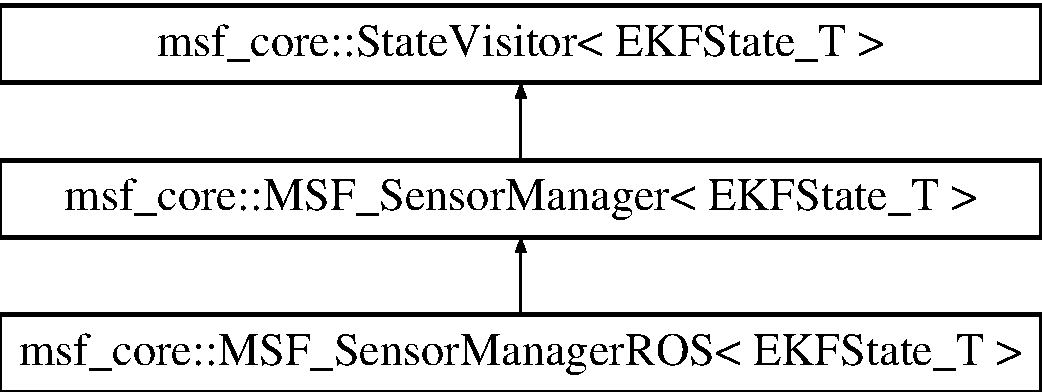
\includegraphics[height=3.000000cm]{structmsf__core_1_1MSF__SensorManagerROS}
\end{center}
\end{figure}
\subsection*{Public Member Functions}
\begin{DoxyCompactItemize}
\item 
\hypertarget{structmsf__core_1_1MSF__SensorManagerROS_a1d665e46ae9945ab6a129575c4400bd3}{E\-I\-G\-E\-N\-\_\-\-M\-A\-K\-E\-\_\-\-A\-L\-I\-G\-N\-E\-D\-\_\-\-O\-P\-E\-R\-A\-T\-O\-R\-\_\-\-N\-E\-W {\bfseries M\-S\-F\-\_\-\-Sensor\-Manager\-R\-O\-S} (ros\-::\-Node\-Handle pnh=ros\-::\-Node\-Handle(\char`\"{}$\sim$core\char`\"{}))}\label{structmsf__core_1_1MSF__SensorManagerROS_a1d665e46ae9945ab6a129575c4400bd3}

\item 
\hypertarget{structmsf__core_1_1MSF__SensorManagerROS_a092e5cecd4d0586303c0412e55959603}{virtual void \hyperlink{structmsf__core_1_1MSF__SensorManagerROS_a092e5cecd4d0586303c0412e55959603}{core\-Config} (msf\-\_\-core\-::\-M\-S\-F\-\_\-\-Core\-Config \&config, uint32\-\_\-t level)}\label{structmsf__core_1_1MSF__SensorManagerROS_a092e5cecd4d0586303c0412e55959603}

\begin{DoxyCompactList}\small\item\em Gets called by the internal callback caller. \end{DoxyCompactList}\item 
\hypertarget{structmsf__core_1_1MSF__SensorManagerROS_a05d1f96502e2733ac5d9810f4dd55706}{void \hyperlink{structmsf__core_1_1MSF__SensorManagerROS_a05d1f96502e2733ac5d9810f4dd55706}{Config} (msf\-\_\-core\-::\-M\-S\-F\-\_\-\-Core\-Config \&config, uint32\-\_\-t level)}\label{structmsf__core_1_1MSF__SensorManagerROS_a05d1f96502e2733ac5d9810f4dd55706}

\begin{DoxyCompactList}\small\item\em Gets called by dynamic reconfigure and calls all registered callbacks in callbacks\-\_\-. \end{DoxyCompactList}\item 
\hypertarget{structmsf__core_1_1MSF__SensorManagerROS_a4b28905e8303ca5d74a2711c6483329c}{void {\bfseries set\-H\-L\-State\-Buffer} (const sensor\-\_\-fusion\-\_\-comm\-::\-Ext\-Ekf \&msg)}\label{structmsf__core_1_1MSF__SensorManagerROS_a4b28905e8303ca5d74a2711c6483329c}

\item 
\hypertarget{structmsf__core_1_1MSF__SensorManagerROS_a25e296341f9628b7e0c5616d09b1830b}{virtual bool {\bfseries get\-Param\-\_\-fixed\-\_\-bias} () const }\label{structmsf__core_1_1MSF__SensorManagerROS_a25e296341f9628b7e0c5616d09b1830b}

\item 
\hypertarget{structmsf__core_1_1MSF__SensorManagerROS_a8832a1f48d484a04120c32bf1ffa2b63}{virtual double {\bfseries get\-Param\-\_\-noise\-\_\-acc} () const }\label{structmsf__core_1_1MSF__SensorManagerROS_a8832a1f48d484a04120c32bf1ffa2b63}

\item 
\hypertarget{structmsf__core_1_1MSF__SensorManagerROS_a73d7709e65b947e02a8080b65c6d3e7a}{virtual double {\bfseries get\-Param\-\_\-noise\-\_\-accbias} () const }\label{structmsf__core_1_1MSF__SensorManagerROS_a73d7709e65b947e02a8080b65c6d3e7a}

\item 
\hypertarget{structmsf__core_1_1MSF__SensorManagerROS_aedf81899b9210ba2d869f1b66f4e6ee0}{virtual double {\bfseries get\-Param\-\_\-noise\-\_\-gyr} () const }\label{structmsf__core_1_1MSF__SensorManagerROS_aedf81899b9210ba2d869f1b66f4e6ee0}

\item 
\hypertarget{structmsf__core_1_1MSF__SensorManagerROS_a5dad5d6ad078af02bf85ca5edd871a0b}{virtual double {\bfseries get\-Param\-\_\-noise\-\_\-gyrbias} () const }\label{structmsf__core_1_1MSF__SensorManagerROS_a5dad5d6ad078af02bf85ca5edd871a0b}

\item 
\hypertarget{structmsf__core_1_1MSF__SensorManagerROS_a40d9507b8a2a513b70078583c4851995}{virtual double {\bfseries get\-Param\-\_\-fuzzythres} () const }\label{structmsf__core_1_1MSF__SensorManagerROS_a40d9507b8a2a513b70078583c4851995}

\item 
virtual void \hyperlink{structmsf__core_1_1MSF__SensorManagerROS_abde229602f1aeb393a2aad30ef413e12}{publish\-State\-Initial} (const shared\-\_\-ptr$<$ E\-K\-F\-State\-\_\-\-T $>$ \&state) const 
\item 
\hypertarget{structmsf__core_1_1MSF__SensorManagerROS_abcf566a97988f986deb36b5c7b2d8248}{virtual void {\bfseries publish\-State\-After\-Propagation} (const shared\-\_\-ptr$<$ E\-K\-F\-State\-\_\-\-T $>$ \&state) const }\label{structmsf__core_1_1MSF__SensorManagerROS_abcf566a97988f986deb36b5c7b2d8248}

\item 
\hypertarget{structmsf__core_1_1MSF__SensorManagerROS_a612d69d5e10b3d6de0eed6e4c6720afa}{virtual void {\bfseries publish\-State\-After\-Update} (const shared\-\_\-ptr$<$ E\-K\-F\-State\-\_\-\-T $>$ \&state) const }\label{structmsf__core_1_1MSF__SensorManagerROS_a612d69d5e10b3d6de0eed6e4c6720afa}

\end{DoxyCompactItemize}
\subsection*{Protected Attributes}
\begin{DoxyCompactItemize}
\item 
\hypertarget{structmsf__core_1_1MSF__SensorManagerROS_aa35b7b94cdf025302d7f980f2e68f413}{msf\-\_\-core\-::\-M\-S\-F\-\_\-\-Core\-Config \hyperlink{structmsf__core_1_1MSF__SensorManagerROS_aa35b7b94cdf025302d7f980f2e68f413}{config\-\_\-}}\label{structmsf__core_1_1MSF__SensorManagerROS_aa35b7b94cdf025302d7f980f2e68f413}

\begin{DoxyCompactList}\small\item\em Dynamic reconfigure config. \end{DoxyCompactList}\end{DoxyCompactItemize}
\subsection*{Additional Inherited Members}


\subsection{Detailed Description}
\subsubsection*{template$<$typename E\-K\-F\-State\-\_\-\-T$>$class msf\-\_\-core\-::\-M\-S\-F\-\_\-\-Sensor\-Manager\-R\-O\-S$<$ E\-K\-F\-State\-\_\-\-T $>$}

Abstract class defining user configurable calculations for the msf\-\_\-core with R\-O\-S interfaces. 

\subsection{Member Function Documentation}
\hypertarget{structmsf__core_1_1MSF__SensorManagerROS_abde229602f1aeb393a2aad30ef413e12}{\index{msf\-\_\-core\-::\-M\-S\-F\-\_\-\-Sensor\-Manager\-R\-O\-S@{msf\-\_\-core\-::\-M\-S\-F\-\_\-\-Sensor\-Manager\-R\-O\-S}!publish\-State\-Initial@{publish\-State\-Initial}}
\index{publish\-State\-Initial@{publish\-State\-Initial}!msf_core::MSF_SensorManagerROS@{msf\-\_\-core\-::\-M\-S\-F\-\_\-\-Sensor\-Manager\-R\-O\-S}}
\subsubsection[{publish\-State\-Initial}]{\setlength{\rightskip}{0pt plus 5cm}template$<$typename E\-K\-F\-State\-\_\-\-T $>$ virtual void {\bf msf\-\_\-core\-::\-M\-S\-F\-\_\-\-Sensor\-Manager\-R\-O\-S}$<$ E\-K\-F\-State\-\_\-\-T $>$\-::publish\-State\-Initial (
\begin{DoxyParamCaption}
\item[{const shared\-\_\-ptr$<$ E\-K\-F\-State\-\_\-\-T $>$ \&}]{state}
\end{DoxyParamCaption}
) const\hspace{0.3cm}{\ttfamily [inline]}, {\ttfamily [virtual]}}}\label{structmsf__core_1_1MSF__SensorManagerROS_abde229602f1aeb393a2aad30ef413e12}
This functions get called by the core to publish data to external middlewares like R\-O\-S. Initialize the H\-L\-P based propagation. 
\begin{DoxyParams}{Parameters}
{\em State} & the state to send to the H\-L\-P.\\
\hline
\end{DoxyParams}


Implements \hyperlink{classmsf__core_1_1MSF__SensorManager_ad851fff1bceaeb6696ef79a4792a317a}{msf\-\_\-core\-::\-M\-S\-F\-\_\-\-Sensor\-Manager$<$ E\-K\-F\-State\-\_\-\-T $>$}.



The documentation for this class was generated from the following file\-:\begin{DoxyCompactItemize}
\item 
msf\-\_\-core/include/msf\-\_\-core/msf\-\_\-sensormanager\-R\-O\-S.\-h\end{DoxyCompactItemize}

\hypertarget{structmsf__tmp_1_1overflow}{\section{msf\-\_\-tmp\-:\-:overflow$<$ size $>$ Struct Template Reference}
\label{structmsf__tmp_1_1overflow}\index{msf\-\_\-tmp\-::overflow$<$ size $>$@{msf\-\_\-tmp\-::overflow$<$ size $>$}}
}


Output a compile time constant by overflowing a char, producing a warning.  




{\ttfamily \#include $<$msf\-\_\-tmp.\-h$>$}

\subsection*{Public Member Functions}
\begin{DoxyCompactItemize}
\item 
\hyperlink{structmsf__tmp_1_1overflow_a4876303a7c2e84a69671b61e24ed2b8f}{operator char} ()
\end{DoxyCompactItemize}


\subsection{Member Function Documentation}
\hypertarget{structmsf__tmp_1_1overflow_a4876303a7c2e84a69671b61e24ed2b8f}{\index{msf\-\_\-tmp\-::overflow@{msf\-\_\-tmp\-::overflow}!operator char@{operator char}}
\index{operator char@{operator char}!msf_tmp::overflow@{msf\-\_\-tmp\-::overflow}}
\subsubsection[{operator char}]{\setlength{\rightskip}{0pt plus 5cm}template$<$size\-\_\-t size$>$ {\bf msf\-\_\-tmp\-::overflow}$<$ size $>$\-::operator char (
\begin{DoxyParamCaption}
{}
\end{DoxyParamCaption}
)\hspace{0.3cm}{\ttfamily [inline]}}}\label{structmsf__tmp_1_1overflow_a4876303a7c2e84a69671b61e24ed2b8f}


The documentation for this struct was generated from the following file\-:\begin{DoxyCompactItemize}
\item 
msf\-\_\-core/include/msf\-\_\-core/\hyperlink{msf__tmp_8h}{msf\-\_\-tmp.\-h}\end{DoxyCompactItemize}

\hypertarget{structpalette}{\section{palette Struct Reference}
\label{structpalette}\index{palette@{palette}}
}
\subsection*{Public Types}
\begin{DoxyCompactItemize}
\item 
enum {\bfseries palettetypes} \{ \\*
{\bfseries Linear\-\_\-red\-\_\-palettes}, 
{\bfseries Gamma\-Log\-\_\-red\-\_\-palettes}, 
{\bfseries Inversion\-\_\-red\-\_\-palette}, 
{\bfseries Linear\-\_\-palettes}, 
\\*
{\bfseries Gamma\-Log\-\_\-palettes}, 
{\bfseries Inversion\-\_\-palette}, 
{\bfseries False\-\_\-color\-\_\-palette1}, 
{\bfseries False\-\_\-color\-\_\-palette2}, 
\\*
{\bfseries False\-\_\-color\-\_\-palette3}, 
{\bfseries False\-\_\-color\-\_\-palette4}
 \}
\end{DoxyCompactItemize}
\subsection*{Public Attributes}
\begin{DoxyCompactItemize}
\item 
\hypertarget{structpalette_aa1a2941bd65472f07de5e54bcf36678b}{\hyperlink{structcolor}{color} {\bfseries colors} \mbox{[}256\mbox{]}}\label{structpalette_aa1a2941bd65472f07de5e54bcf36678b}

\end{DoxyCompactItemize}


The documentation for this struct was generated from the following file\-:\begin{DoxyCompactItemize}
\item 
msf\-\_\-core/include/msf\-\_\-core/falsecolor.\-h\end{DoxyCompactItemize}

\hypertarget{structmsf__tmp_1_1resetState}{\section{msf\-\_\-tmp\-:\-:reset\-State Struct Reference}
\label{structmsf__tmp_1_1resetState}\index{msf\-\_\-tmp\-::reset\-State@{msf\-\_\-tmp\-::reset\-State}}
}


Reset the E\-K\-F state in a boost fusion unrolled call.  




{\ttfamily \#include $<$msf\-\_\-tmp.\-h$>$}

\subsection*{Public Member Functions}
\begin{DoxyCompactItemize}
\item 
{\footnotesize template$<$int N\-A\-M\-E, int N, int S\-T\-A\-T\-E\-\_\-\-T, int O\-P\-T\-I\-O\-N\-S$>$ }\\void \hyperlink{structmsf__tmp_1_1resetState_aa7e3525c8c9777ba163da0f64872eaca}{operator()} (\hyperlink{structmsf__core_1_1StateVar__T}{msf\-\_\-core\-::\-State\-Var\-\_\-\-T}$<$ Eigen\-::\-Matrix$<$ double, N, 1 $>$, N\-A\-M\-E, S\-T\-A\-T\-E\-\_\-\-T, O\-P\-T\-I\-O\-N\-S $>$ \&t) const 
\item 
{\footnotesize template$<$int N\-A\-M\-E, int S\-T\-A\-T\-E\-\_\-\-T, int O\-P\-T\-I\-O\-N\-S$>$ }\\void \hyperlink{structmsf__tmp_1_1resetState_af31c01964acef3d4a598ee139b9e7013}{operator()} (\hyperlink{structmsf__core_1_1StateVar__T}{msf\-\_\-core\-::\-State\-Var\-\_\-\-T}$<$ Eigen\-::\-Quaterniond, N\-A\-M\-E, S\-T\-A\-T\-E\-\_\-\-T, O\-P\-T\-I\-O\-N\-S $>$ \&t) const 
\end{DoxyCompactItemize}


\subsection{Member Function Documentation}
\hypertarget{structmsf__tmp_1_1resetState_aa7e3525c8c9777ba163da0f64872eaca}{\index{msf\-\_\-tmp\-::reset\-State@{msf\-\_\-tmp\-::reset\-State}!operator()@{operator()}}
\index{operator()@{operator()}!msf_tmp::resetState@{msf\-\_\-tmp\-::reset\-State}}
\subsubsection[{operator()}]{\setlength{\rightskip}{0pt plus 5cm}template$<$int N\-A\-M\-E, int N, int S\-T\-A\-T\-E\-\_\-\-T, int O\-P\-T\-I\-O\-N\-S$>$ void msf\-\_\-tmp\-::reset\-State\-::operator() (
\begin{DoxyParamCaption}
\item[{{\bf msf\-\_\-core\-::\-State\-Var\-\_\-\-T}$<$ Eigen\-::\-Matrix$<$ double, N, 1 $>$, N\-A\-M\-E, S\-T\-A\-T\-E\-\_\-\-T, O\-P\-T\-I\-O\-N\-S $>$ \&}]{t}
\end{DoxyParamCaption}
) const\hspace{0.3cm}{\ttfamily [inline]}}}\label{structmsf__tmp_1_1resetState_aa7e3525c8c9777ba163da0f64872eaca}
\hypertarget{structmsf__tmp_1_1resetState_af31c01964acef3d4a598ee139b9e7013}{\index{msf\-\_\-tmp\-::reset\-State@{msf\-\_\-tmp\-::reset\-State}!operator()@{operator()}}
\index{operator()@{operator()}!msf_tmp::resetState@{msf\-\_\-tmp\-::reset\-State}}
\subsubsection[{operator()}]{\setlength{\rightskip}{0pt plus 5cm}template$<$int N\-A\-M\-E, int S\-T\-A\-T\-E\-\_\-\-T, int O\-P\-T\-I\-O\-N\-S$>$ void msf\-\_\-tmp\-::reset\-State\-::operator() (
\begin{DoxyParamCaption}
\item[{{\bf msf\-\_\-core\-::\-State\-Var\-\_\-\-T}$<$ Eigen\-::\-Quaterniond, N\-A\-M\-E, S\-T\-A\-T\-E\-\_\-\-T, O\-P\-T\-I\-O\-N\-S $>$ \&}]{t}
\end{DoxyParamCaption}
) const\hspace{0.3cm}{\ttfamily [inline]}}}\label{structmsf__tmp_1_1resetState_af31c01964acef3d4a598ee139b9e7013}


The documentation for this struct was generated from the following file\-:\begin{DoxyCompactItemize}
\item 
msf\-\_\-core/include/msf\-\_\-core/\hyperlink{msf__tmp_8h}{msf\-\_\-tmp.\-h}\end{DoxyCompactItemize}

\hypertarget{structmsf__tmp_1_1SameType}{\section{msf\-\_\-tmp\-:\-:Same\-Type$<$ T, U $>$ Struct Template Reference}
\label{structmsf__tmp_1_1SameType}\index{msf\-\_\-tmp\-::\-Same\-Type$<$ T, U $>$@{msf\-\_\-tmp\-::\-Same\-Type$<$ T, U $>$}}
}


{\ttfamily \#include $<$msf\-\_\-typetraits.\-hpp$>$}

\subsection*{Public Types}
\begin{DoxyCompactItemize}
\item 
enum \{ \hyperlink{structmsf__tmp_1_1SameType_af6f7567ca10c06b552e2714d37d3d868a649157a456919a298d1703c45117e197}{value} =  false
 \}
\end{DoxyCompactItemize}


\subsection{Member Enumeration Documentation}
\hypertarget{structmsf__tmp_1_1SameType_af6f7567ca10c06b552e2714d37d3d868}{\subsubsection[{anonymous enum}]{\setlength{\rightskip}{0pt plus 5cm}template$<$typename T , typename U $>$ anonymous enum}}\label{structmsf__tmp_1_1SameType_af6f7567ca10c06b552e2714d37d3d868}
\begin{Desc}
\item[Enumerator\-: ]\par
\begin{description}
\index{value@{value}!msf\-\_\-tmp\-::\-Same\-Type@{msf\-\_\-tmp\-::\-Same\-Type}}\index{msf\-\_\-tmp\-::\-Same\-Type@{msf\-\_\-tmp\-::\-Same\-Type}!value@{value}}\item[{\em 
\hypertarget{structmsf__tmp_1_1SameType_af6f7567ca10c06b552e2714d37d3d868a649157a456919a298d1703c45117e197}{value}\label{structmsf__tmp_1_1SameType_af6f7567ca10c06b552e2714d37d3d868a649157a456919a298d1703c45117e197}
}]\end{description}
\end{Desc}



The documentation for this struct was generated from the following file\-:\begin{DoxyCompactItemize}
\item 
msf\-\_\-core/include/msf\-\_\-core/\hyperlink{msf__typetraits_8hpp}{msf\-\_\-typetraits.\-hpp}\end{DoxyCompactItemize}

\hypertarget{structmsf__tmp_1_1SameType_3_01T_00_01T_01_4}{\section{msf\-\_\-tmp\-:\-:Same\-Type$<$ T, T $>$ Struct Template Reference}
\label{structmsf__tmp_1_1SameType_3_01T_00_01T_01_4}\index{msf\-\_\-tmp\-::\-Same\-Type$<$ T, T $>$@{msf\-\_\-tmp\-::\-Same\-Type$<$ T, T $>$}}
}
\subsection*{Public Types}
\begin{DoxyCompactItemize}
\item 
enum \{ {\bfseries value} =  true
 \}
\end{DoxyCompactItemize}


The documentation for this struct was generated from the following file\-:\begin{DoxyCompactItemize}
\item 
msf\-\_\-core/include/msf\-\_\-core/msf\-\_\-typetraits.\-hpp\end{DoxyCompactItemize}

\hypertarget{classmsf__core_1_1SensorHandler}{\section{msf\-\_\-core\-:\-:Sensor\-Handler$<$ E\-K\-F\-State\-\_\-\-T $>$ Class Template Reference}
\label{classmsf__core_1_1SensorHandler}\index{msf\-\_\-core\-::\-Sensor\-Handler$<$ E\-K\-F\-State\-\_\-\-T $>$@{msf\-\_\-core\-::\-Sensor\-Handler$<$ E\-K\-F\-State\-\_\-\-T $>$}}
}


Handles a sensor driver which provides the sensor readings.  




{\ttfamily \#include $<$msf\-\_\-sensorhandler.\-h$>$}

Inheritance diagram for msf\-\_\-core\-:\-:Sensor\-Handler$<$ E\-K\-F\-State\-\_\-\-T $>$\-:\begin{figure}[H]
\begin{center}
\leavevmode
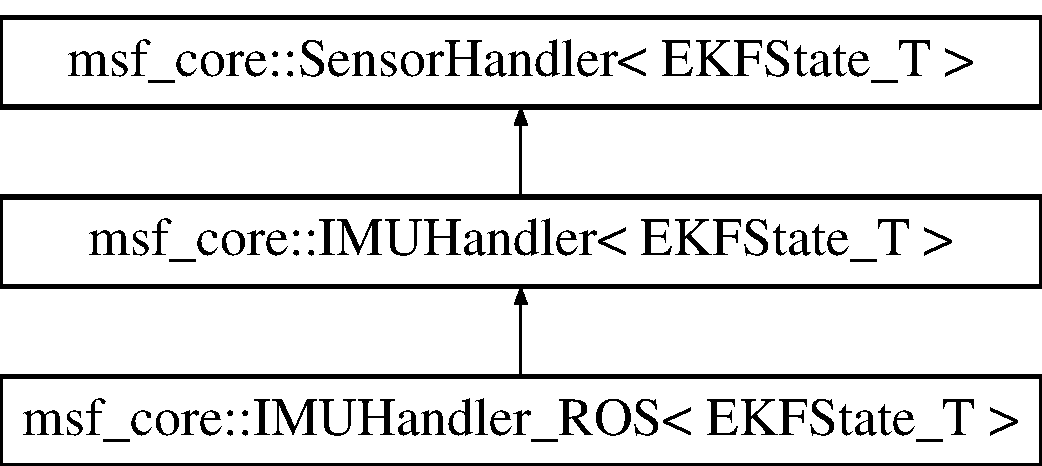
\includegraphics[height=3.000000cm]{classmsf__core_1_1SensorHandler}
\end{center}
\end{figure}
\subsection*{Public Member Functions}
\begin{DoxyCompactItemize}
\item 
\hypertarget{classmsf__core_1_1SensorHandler_aba1cd2f28ff92d5005ab7ad006e20023}{{\bfseries Sensor\-Handler} (\hyperlink{classmsf__core_1_1MSF__SensorManager}{M\-S\-F\-\_\-\-Sensor\-Manager}$<$ E\-K\-F\-State\-\_\-\-T $>$ \&mng, const std\-::string \&topic\-\_\-namespace, const std\-::string \&parameternamespace)}\label{classmsf__core_1_1SensorHandler_aba1cd2f28ff92d5005ab7ad006e20023}

\end{DoxyCompactItemize}
\subsection*{Public Attributes}
\begin{DoxyCompactItemize}
\item 
\hypertarget{classmsf__core_1_1SensorHandler_ab25601f461c0c7e0e898f8eb200ec2b6}{{\bfseries E\-I\-G\-E\-N\-\_\-\-M\-A\-K\-E\-\_\-\-A\-L\-I\-G\-N\-E\-D\-\_\-\-O\-P\-E\-R\-A\-T\-O\-R\-\_\-\-N\-E\-W}}\label{classmsf__core_1_1SensorHandler_ab25601f461c0c7e0e898f8eb200ec2b6}

\end{DoxyCompactItemize}
\subsection*{Protected Member Functions}
\begin{DoxyCompactItemize}
\item 
\hypertarget{classmsf__core_1_1SensorHandler_acf0819310dd6421128da97a216523036}{void {\bfseries set\-Sensor\-I\-D} (int I\-D)}\label{classmsf__core_1_1SensorHandler_acf0819310dd6421128da97a216523036}

\item 
\hypertarget{classmsf__core_1_1SensorHandler_a96a37204ef5281f0cc195f22c211563e}{void {\bfseries sequence\-Watch\-Dog} (size\-\_\-t seq, const std\-::string \&topic)}\label{classmsf__core_1_1SensorHandler_a96a37204ef5281f0cc195f22c211563e}

\end{DoxyCompactItemize}
\subsection*{Protected Attributes}
\begin{DoxyCompactItemize}
\item 
\hypertarget{classmsf__core_1_1SensorHandler_aa5b9c6d345c1d2d809f7d53a0c212bf4}{\hyperlink{classmsf__core_1_1MSF__SensorManager}{M\-S\-F\-\_\-\-Sensor\-Manager}$<$ E\-K\-F\-State\-\_\-\-T $>$ \& {\bfseries manager\-\_\-}}\label{classmsf__core_1_1SensorHandler_aa5b9c6d345c1d2d809f7d53a0c212bf4}

\item 
\hypertarget{classmsf__core_1_1SensorHandler_ab6b02c25292da4a56ff7ebf3edb1b17b}{int {\bfseries sensor\-I\-D}}\label{classmsf__core_1_1SensorHandler_ab6b02c25292da4a56ff7ebf3edb1b17b}

\item 
\hypertarget{classmsf__core_1_1SensorHandler_a7795149ef5cef567fcc049bbc888c9ed}{std\-::string {\bfseries topic\-\_\-namespace\-\_\-}}\label{classmsf__core_1_1SensorHandler_a7795149ef5cef567fcc049bbc888c9ed}

\item 
\hypertarget{classmsf__core_1_1SensorHandler_a1be62365d3ce3c6cbfcca2e4e453790f}{std\-::string {\bfseries parameternamespace\-\_\-}}\label{classmsf__core_1_1SensorHandler_a1be62365d3ce3c6cbfcca2e4e453790f}

\end{DoxyCompactItemize}
\subsection*{Friends}
\begin{DoxyCompactItemize}
\item 
\hypertarget{classmsf__core_1_1SensorHandler_a8af2d8b87c3570c0ee69b7e0f4ea5077}{class {\bfseries M\-S\-F\-\_\-\-Sensor\-Manager$<$ E\-K\-F\-State\-\_\-\-T $>$}}\label{classmsf__core_1_1SensorHandler_a8af2d8b87c3570c0ee69b7e0f4ea5077}

\end{DoxyCompactItemize}


\subsection{Detailed Description}
\subsubsection*{template$<$typename E\-K\-F\-State\-\_\-\-T$>$class msf\-\_\-core\-::\-Sensor\-Handler$<$ E\-K\-F\-State\-\_\-\-T $>$}

Handles a sensor driver which provides the sensor readings. 

The documentation for this class was generated from the following file\-:\begin{DoxyCompactItemize}
\item 
msf\-\_\-core/include/msf\-\_\-core/msf\-\_\-sensorhandler.\-h\end{DoxyCompactItemize}

\hypertarget{classmsf__core_1_1SortedContainer}{\section{msf\-\_\-core\-:\-:Sorted\-Container$<$ T, Prototype\-Invalid\-T $>$ Class Template Reference}
\label{classmsf__core_1_1SortedContainer}\index{msf\-\_\-core\-::\-Sorted\-Container$<$ T, Prototype\-Invalid\-T $>$@{msf\-\_\-core\-::\-Sorted\-Container$<$ T, Prototype\-Invalid\-T $>$}}
}


Manages a sorted container with strict less than ordering used to store state and measurement objects which can then be queried for closest states/measurements to a given time instant.  




{\ttfamily \#include $<$msf\-\_\-sorted\-Container.\-h$>$}

\subsection*{Public Types}
\begin{DoxyCompactItemize}
\item 
typedef shared\-\_\-ptr$<$ T $>$ \hyperlink{classmsf__core_1_1SortedContainer_a0dd7e9676bf540e11f526a8ac16da06b}{Ptr\-\_\-\-T}
\item 
typedef List\-T\-::iterator \hyperlink{classmsf__core_1_1SortedContainer_ac060dafe3a40d73ef6d35f4be7e0213e}{iterator\-\_\-\-T}
\end{DoxyCompactItemize}
\subsection*{Public Member Functions}
\begin{DoxyCompactItemize}
\item 
\hyperlink{classmsf__core_1_1SortedContainer_a92fa629150b579414169ce689fa2f168}{Sorted\-Container} ()
\item 
shared\-\_\-ptr$<$ T $>$ \& \hyperlink{classmsf__core_1_1SortedContainer_a9c72942ce59c634559fe7e226b6ab302}{get\-Invalid} ()
\begin{DoxyCompactList}\small\item\em To be called to signal that a request could not be satisfied. \end{DoxyCompactList}\item 
void \hyperlink{classmsf__core_1_1SortedContainer_aea65ad1ff460ab46445b433ea3db49b1}{clear} ()
\begin{DoxyCompactList}\small\item\em Clears the internal container, dropping all the contents. \end{DoxyCompactList}\item 
List\-T\-::size\-\_\-type \hyperlink{classmsf__core_1_1SortedContainer_af51c989973b49002e737190cec67b6b4}{size} ()
\begin{DoxyCompactList}\small\item\em Returns the size of the internal container. \end{DoxyCompactList}\item 
List\-T\-::iterator \hyperlink{classmsf__core_1_1SortedContainer_a8e6ef89431cbcac53439b580a7b8706c}{insert} (const shared\-\_\-ptr$<$ T $>$ \&value)
\begin{DoxyCompactList}\small\item\em Insert an object to the internal container to the position not violating the internal strict less than ordering by time. \end{DoxyCompactList}\item 
List\-T\-::iterator \hyperlink{classmsf__core_1_1SortedContainer_a66c37f04293ec2b3e2fae69ff2ac498e}{get\-Iterator\-Begin} ()
\begin{DoxyCompactList}\small\item\em Returns the iterator at the beginning of the internal container. \end{DoxyCompactList}\item 
List\-T\-::iterator \hyperlink{classmsf__core_1_1SortedContainer_a17fa1667d94905e8def74a65002907ed}{get\-Iterator\-Before\-Begin} ()
\begin{DoxyCompactList}\small\item\em Returns the iterator before the beginning of the internal container. \end{DoxyCompactList}\item 
List\-T\-::iterator \hyperlink{classmsf__core_1_1SortedContainer_af1b1597192ac889cc918d8516cd6345c}{get\-Iterator\-End} ()
\begin{DoxyCompactList}\small\item\em Returns the iterator at the end of the internal container. \end{DoxyCompactList}\item 
List\-T\-::iterator \hyperlink{classmsf__core_1_1SortedContainer_a3ca27ff6fae8916a88a6690b9c8365a9}{get\-Iterator\-At\-Value} (const shared\-\_\-ptr$<$ T $>$ \&value, bool warn\-If\-Not\-Existant=true)
\begin{DoxyCompactList}\small\item\em Returns the iterator at the specific time instant of the supplied object or an invalid object if the request cannot be satisfied. \end{DoxyCompactList}\item 
List\-T\-::iterator \hyperlink{classmsf__core_1_1SortedContainer_a727a60e4eb00ab45b2a39c8c069d2fcf}{get\-Iterator\-At\-Value} (const double \&time, bool warn\-If\-Not\-Existant=true)
\begin{DoxyCompactList}\small\item\em Returns the iterator at a specific time instant or an invalid object if the request cannot be satisfied. \end{DoxyCompactList}\item 
List\-T\-::iterator \hyperlink{classmsf__core_1_1SortedContainer_a4cbd2aeae2f6dde2dfd0dceea4a8e928}{get\-Iterator\-Closest\-Before} (const double \&statetime)
\begin{DoxyCompactList}\small\item\em Returns the iterator closest before a specific time instant. \end{DoxyCompactList}\item 
List\-T\-::iterator \hyperlink{classmsf__core_1_1SortedContainer_a3c1f848e9874f9bdc4ab12645e699fcf}{get\-Iterator\-Closest\-After} (const double \&statetime)
\begin{DoxyCompactList}\small\item\em Returns the iterator closest after a specific time instant. \end{DoxyCompactList}\item 
List\-T\-::iterator \hyperlink{classmsf__core_1_1SortedContainer_a64ce9fdfdd6220f78187e7270f689f02}{get\-Iterator\-Closest} (const double \&statetime)
\begin{DoxyCompactList}\small\item\em Returns the iterator closest to a specific time instant. \end{DoxyCompactList}\item 
shared\-\_\-ptr$<$ T $>$ \& \hyperlink{classmsf__core_1_1SortedContainer_ad027825ff0a1360acbe6b9c60f708cd9}{get\-Closest\-Before} (const double \&statetime)
\begin{DoxyCompactList}\small\item\em Returns a pointer to the closest object before a specific time instant. \end{DoxyCompactList}\item 
shared\-\_\-ptr$<$ T $>$ \& \hyperlink{classmsf__core_1_1SortedContainer_a1bf7a97e06b2dd5bc2b6588dcb6799b8}{get\-Closest\-After} (const double \&statetime)
\begin{DoxyCompactList}\small\item\em Returns a pointer to the closest after a specific time instant or an invalid object if the request cannot be satisfied. \end{DoxyCompactList}\item 
shared\-\_\-ptr$<$ T $>$ \& \hyperlink{classmsf__core_1_1SortedContainer_aa0de5fa4d79a266a36556b67252a7d34}{get\-Value\-At} (const double \&statetime)
\begin{DoxyCompactList}\small\item\em Returns a pointer to the object at a specific time instant or an invalid object if the request cannot be satisfied. \end{DoxyCompactList}\item 
shared\-\_\-ptr$<$ T $>$ \& \hyperlink{classmsf__core_1_1SortedContainer_ab262e5e5904b047df44110c1d05babdc}{get\-Closest} (const double \&statetime)
\begin{DoxyCompactList}\small\item\em Returns a pointer to the closest to a specific time instant. \end{DoxyCompactList}\item 
void \hyperlink{classmsf__core_1_1SortedContainer_aa2e690d22ea362eeb281ce30a96751d5}{clear\-Older\-Than} (double age)
\begin{DoxyCompactList}\small\item\em Clears all objects having a time stamp older than the supplied time in seconds. \end{DoxyCompactList}\item 
shared\-\_\-ptr$<$ T $>$ \& \hyperlink{classmsf__core_1_1SortedContainer_ada83f9baa4b17b5816975b1e67354ff1}{get\-Last} ()
\begin{DoxyCompactList}\small\item\em Returns a pointer to the last object in the container or an invalid object if the container is empty. \end{DoxyCompactList}\item 
shared\-\_\-ptr$<$ T $>$ \& \hyperlink{classmsf__core_1_1SortedContainer_a7cce297c5a4bbf80d617741fe3dc902e}{get\-First} ()
\begin{DoxyCompactList}\small\item\em Returns a pointer to the first object in the container or an invalid object if the container is empty. \end{DoxyCompactList}\item 
shared\-\_\-ptr$<$ T $>$ \hyperlink{classmsf__core_1_1SortedContainer_a7e4c594bb1aec9d6d4d8fb73e7baff9a}{update\-Time} (double time\-Old, double time\-New) \-\_\-\-\_\-attribute\-\_\-\-\_\-((warn\-\_\-unused\-\_\-result))
\begin{DoxyCompactList}\small\item\em This function updates the time of an object in the container this function effectively changes the map ordering, so the previous iterators are invalidated the attribute unused can be eliminated for non gcc compilers, its just a little more verbose in cases where the updated value is not used. \end{DoxyCompactList}\item 
std\-::string \hyperlink{classmsf__core_1_1SortedContainer_a7cecf8583999a5b457e04d5ef781dc5d}{echo\-Buffer\-Content\-Times} ()
\begin{DoxyCompactList}\small\item\em Debug output the contents of the container in a human readable time format. \end{DoxyCompactList}\end{DoxyCompactItemize}
\subsection*{Private Types}
\begin{DoxyCompactItemize}
\item 
typedef std\-::map$<$ double, \hyperlink{classmsf__core_1_1SortedContainer_a0dd7e9676bf540e11f526a8ac16da06b}{Ptr\-\_\-\-T} $>$ \hyperlink{classmsf__core_1_1SortedContainer_abb7bb5ff6c1a1916b8c7e48a50953919}{List\-T}
\begin{DoxyCompactList}\small\item\em The container type in which to store the data. \end{DoxyCompactList}\end{DoxyCompactItemize}
\subsection*{Private Attributes}
\begin{DoxyCompactItemize}
\item 
\hyperlink{classmsf__core_1_1SortedContainer_abb7bb5ff6c1a1916b8c7e48a50953919}{List\-T} \hyperlink{classmsf__core_1_1SortedContainer_af9bdeecb0097b80a202d5edd044ffda4}{state\-List}
\begin{DoxyCompactList}\small\item\em The container in which all the data is stored. \end{DoxyCompactList}\item 
\hyperlink{classmsf__core_1_1SortedContainer_a0dd7e9676bf540e11f526a8ac16da06b}{Ptr\-\_\-\-T} \hyperlink{classmsf__core_1_1SortedContainer_a60a2f66705f0a77095e763f7dbe2e265}{invalid}
\begin{DoxyCompactList}\small\item\em A object to signal requests which cannot be satisfied. \end{DoxyCompactList}\end{DoxyCompactItemize}


\subsection{Member Typedef Documentation}
\hypertarget{classmsf__core_1_1SortedContainer_ac060dafe3a40d73ef6d35f4be7e0213e}{\index{msf\-\_\-core\-::\-Sorted\-Container@{msf\-\_\-core\-::\-Sorted\-Container}!iterator\-\_\-\-T@{iterator\-\_\-\-T}}
\index{iterator\-\_\-\-T@{iterator\-\_\-\-T}!msf_core::SortedContainer@{msf\-\_\-core\-::\-Sorted\-Container}}
\subsubsection[{iterator\-\_\-\-T}]{\setlength{\rightskip}{0pt plus 5cm}template$<$typename T, typename Prototype\-Invalid\-T = T$>$ typedef List\-T\-::iterator {\bf msf\-\_\-core\-::\-Sorted\-Container}$<$ T, Prototype\-Invalid\-T $>$\-::{\bf iterator\-\_\-\-T}}}\label{classmsf__core_1_1SortedContainer_ac060dafe3a40d73ef6d35f4be7e0213e}
\hypertarget{classmsf__core_1_1SortedContainer_abb7bb5ff6c1a1916b8c7e48a50953919}{\index{msf\-\_\-core\-::\-Sorted\-Container@{msf\-\_\-core\-::\-Sorted\-Container}!List\-T@{List\-T}}
\index{List\-T@{List\-T}!msf_core::SortedContainer@{msf\-\_\-core\-::\-Sorted\-Container}}
\subsubsection[{List\-T}]{\setlength{\rightskip}{0pt plus 5cm}template$<$typename T, typename Prototype\-Invalid\-T = T$>$ typedef std\-::map$<$double, {\bf Ptr\-\_\-\-T}$>$ {\bf msf\-\_\-core\-::\-Sorted\-Container}$<$ T, Prototype\-Invalid\-T $>$\-::{\bf List\-T}\hspace{0.3cm}{\ttfamily [private]}}}\label{classmsf__core_1_1SortedContainer_abb7bb5ff6c1a1916b8c7e48a50953919}
\hypertarget{classmsf__core_1_1SortedContainer_a0dd7e9676bf540e11f526a8ac16da06b}{\index{msf\-\_\-core\-::\-Sorted\-Container@{msf\-\_\-core\-::\-Sorted\-Container}!Ptr\-\_\-\-T@{Ptr\-\_\-\-T}}
\index{Ptr\-\_\-\-T@{Ptr\-\_\-\-T}!msf_core::SortedContainer@{msf\-\_\-core\-::\-Sorted\-Container}}
\subsubsection[{Ptr\-\_\-\-T}]{\setlength{\rightskip}{0pt plus 5cm}template$<$typename T, typename Prototype\-Invalid\-T = T$>$ typedef shared\-\_\-ptr$<$T$>$ {\bf msf\-\_\-core\-::\-Sorted\-Container}$<$ T, Prototype\-Invalid\-T $>$\-::{\bf Ptr\-\_\-\-T}}}\label{classmsf__core_1_1SortedContainer_a0dd7e9676bf540e11f526a8ac16da06b}


\subsection{Constructor \& Destructor Documentation}
\hypertarget{classmsf__core_1_1SortedContainer_a92fa629150b579414169ce689fa2f168}{\index{msf\-\_\-core\-::\-Sorted\-Container@{msf\-\_\-core\-::\-Sorted\-Container}!Sorted\-Container@{Sorted\-Container}}
\index{Sorted\-Container@{Sorted\-Container}!msf_core::SortedContainer@{msf\-\_\-core\-::\-Sorted\-Container}}
\subsubsection[{Sorted\-Container}]{\setlength{\rightskip}{0pt plus 5cm}template$<$typename T, typename Prototype\-Invalid\-T = T$>$ {\bf msf\-\_\-core\-::\-Sorted\-Container}$<$ T, Prototype\-Invalid\-T $>$\-::{\bf Sorted\-Container} (
\begin{DoxyParamCaption}
{}
\end{DoxyParamCaption}
)\hspace{0.3cm}{\ttfamily [inline]}}}\label{classmsf__core_1_1SortedContainer_a92fa629150b579414169ce689fa2f168}


\subsection{Member Function Documentation}
\hypertarget{classmsf__core_1_1SortedContainer_aea65ad1ff460ab46445b433ea3db49b1}{\index{msf\-\_\-core\-::\-Sorted\-Container@{msf\-\_\-core\-::\-Sorted\-Container}!clear@{clear}}
\index{clear@{clear}!msf_core::SortedContainer@{msf\-\_\-core\-::\-Sorted\-Container}}
\subsubsection[{clear}]{\setlength{\rightskip}{0pt plus 5cm}template$<$typename T, typename Prototype\-Invalid\-T = T$>$ void {\bf msf\-\_\-core\-::\-Sorted\-Container}$<$ T, Prototype\-Invalid\-T $>$\-::clear (
\begin{DoxyParamCaption}
{}
\end{DoxyParamCaption}
)\hspace{0.3cm}{\ttfamily [inline]}}}\label{classmsf__core_1_1SortedContainer_aea65ad1ff460ab46445b433ea3db49b1}
\hypertarget{classmsf__core_1_1SortedContainer_aa2e690d22ea362eeb281ce30a96751d5}{\index{msf\-\_\-core\-::\-Sorted\-Container@{msf\-\_\-core\-::\-Sorted\-Container}!clear\-Older\-Than@{clear\-Older\-Than}}
\index{clear\-Older\-Than@{clear\-Older\-Than}!msf_core::SortedContainer@{msf\-\_\-core\-::\-Sorted\-Container}}
\subsubsection[{clear\-Older\-Than}]{\setlength{\rightskip}{0pt plus 5cm}template$<$typename T, typename Prototype\-Invalid\-T = T$>$ void {\bf msf\-\_\-core\-::\-Sorted\-Container}$<$ T, Prototype\-Invalid\-T $>$\-::clear\-Older\-Than (
\begin{DoxyParamCaption}
\item[{double}]{age}
\end{DoxyParamCaption}
)\hspace{0.3cm}{\ttfamily [inline]}}}\label{classmsf__core_1_1SortedContainer_aa2e690d22ea362eeb281ce30a96751d5}

\begin{DoxyParams}{Parameters}
{\em time} & The maximum age of states in the container. \\
\hline
\end{DoxyParams}
\begin{DoxyReturn}{Returns}
shared pointer of the object. 
\end{DoxyReturn}
\hypertarget{classmsf__core_1_1SortedContainer_a7cecf8583999a5b457e04d5ef781dc5d}{\index{msf\-\_\-core\-::\-Sorted\-Container@{msf\-\_\-core\-::\-Sorted\-Container}!echo\-Buffer\-Content\-Times@{echo\-Buffer\-Content\-Times}}
\index{echo\-Buffer\-Content\-Times@{echo\-Buffer\-Content\-Times}!msf_core::SortedContainer@{msf\-\_\-core\-::\-Sorted\-Container}}
\subsubsection[{echo\-Buffer\-Content\-Times}]{\setlength{\rightskip}{0pt plus 5cm}template$<$typename T, typename Prototype\-Invalid\-T = T$>$ std\-::string {\bf msf\-\_\-core\-::\-Sorted\-Container}$<$ T, Prototype\-Invalid\-T $>$\-::echo\-Buffer\-Content\-Times (
\begin{DoxyParamCaption}
{}
\end{DoxyParamCaption}
)\hspace{0.3cm}{\ttfamily [inline]}}}\label{classmsf__core_1_1SortedContainer_a7cecf8583999a5b457e04d5ef781dc5d}
\begin{DoxyReturn}{Returns}
String of the buffer contents with line breaks after every entry. 
\end{DoxyReturn}
\hypertarget{classmsf__core_1_1SortedContainer_ab262e5e5904b047df44110c1d05babdc}{\index{msf\-\_\-core\-::\-Sorted\-Container@{msf\-\_\-core\-::\-Sorted\-Container}!get\-Closest@{get\-Closest}}
\index{get\-Closest@{get\-Closest}!msf_core::SortedContainer@{msf\-\_\-core\-::\-Sorted\-Container}}
\subsubsection[{get\-Closest}]{\setlength{\rightskip}{0pt plus 5cm}template$<$typename T, typename Prototype\-Invalid\-T = T$>$ shared\-\_\-ptr$<$T$>$\& {\bf msf\-\_\-core\-::\-Sorted\-Container}$<$ T, Prototype\-Invalid\-T $>$\-::get\-Closest (
\begin{DoxyParamCaption}
\item[{const double \&}]{statetime}
\end{DoxyParamCaption}
)\hspace{0.3cm}{\ttfamily [inline]}}}\label{classmsf__core_1_1SortedContainer_ab262e5e5904b047df44110c1d05babdc}

\begin{DoxyParams}{Parameters}
{\em time} & The time where we want to get the value at. \\
\hline
\end{DoxyParams}
\begin{DoxyReturn}{Returns}
shared pointer of the object. 
\end{DoxyReturn}
\hypertarget{classmsf__core_1_1SortedContainer_a1bf7a97e06b2dd5bc2b6588dcb6799b8}{\index{msf\-\_\-core\-::\-Sorted\-Container@{msf\-\_\-core\-::\-Sorted\-Container}!get\-Closest\-After@{get\-Closest\-After}}
\index{get\-Closest\-After@{get\-Closest\-After}!msf_core::SortedContainer@{msf\-\_\-core\-::\-Sorted\-Container}}
\subsubsection[{get\-Closest\-After}]{\setlength{\rightskip}{0pt plus 5cm}template$<$typename T, typename Prototype\-Invalid\-T = T$>$ shared\-\_\-ptr$<$T$>$\& {\bf msf\-\_\-core\-::\-Sorted\-Container}$<$ T, Prototype\-Invalid\-T $>$\-::get\-Closest\-After (
\begin{DoxyParamCaption}
\item[{const double \&}]{statetime}
\end{DoxyParamCaption}
)\hspace{0.3cm}{\ttfamily [inline]}}}\label{classmsf__core_1_1SortedContainer_a1bf7a97e06b2dd5bc2b6588dcb6799b8}

\begin{DoxyParams}{Parameters}
{\em time} & The time where we want to get the value at \\
\hline
\end{DoxyParams}
\begin{DoxyReturn}{Returns}
shared pointer of the object. 
\end{DoxyReturn}
\hypertarget{classmsf__core_1_1SortedContainer_ad027825ff0a1360acbe6b9c60f708cd9}{\index{msf\-\_\-core\-::\-Sorted\-Container@{msf\-\_\-core\-::\-Sorted\-Container}!get\-Closest\-Before@{get\-Closest\-Before}}
\index{get\-Closest\-Before@{get\-Closest\-Before}!msf_core::SortedContainer@{msf\-\_\-core\-::\-Sorted\-Container}}
\subsubsection[{get\-Closest\-Before}]{\setlength{\rightskip}{0pt plus 5cm}template$<$typename T, typename Prototype\-Invalid\-T = T$>$ shared\-\_\-ptr$<$T$>$\& {\bf msf\-\_\-core\-::\-Sorted\-Container}$<$ T, Prototype\-Invalid\-T $>$\-::get\-Closest\-Before (
\begin{DoxyParamCaption}
\item[{const double \&}]{statetime}
\end{DoxyParamCaption}
)\hspace{0.3cm}{\ttfamily [inline]}}}\label{classmsf__core_1_1SortedContainer_ad027825ff0a1360acbe6b9c60f708cd9}

\begin{DoxyParams}{Parameters}
{\em Time} & the time where we want to get the value at. \\
\hline
\end{DoxyParams}
\begin{DoxyReturn}{Returns}
shared pointer of the object. 
\end{DoxyReturn}
\hypertarget{classmsf__core_1_1SortedContainer_a7cce297c5a4bbf80d617741fe3dc902e}{\index{msf\-\_\-core\-::\-Sorted\-Container@{msf\-\_\-core\-::\-Sorted\-Container}!get\-First@{get\-First}}
\index{get\-First@{get\-First}!msf_core::SortedContainer@{msf\-\_\-core\-::\-Sorted\-Container}}
\subsubsection[{get\-First}]{\setlength{\rightskip}{0pt plus 5cm}template$<$typename T, typename Prototype\-Invalid\-T = T$>$ shared\-\_\-ptr$<$T$>$\& {\bf msf\-\_\-core\-::\-Sorted\-Container}$<$ T, Prototype\-Invalid\-T $>$\-::get\-First (
\begin{DoxyParamCaption}
{}
\end{DoxyParamCaption}
)\hspace{0.3cm}{\ttfamily [inline]}}}\label{classmsf__core_1_1SortedContainer_a7cce297c5a4bbf80d617741fe3dc902e}
\begin{DoxyReturn}{Returns}
shared pointer of the object. 
\end{DoxyReturn}
\hypertarget{classmsf__core_1_1SortedContainer_a9c72942ce59c634559fe7e226b6ab302}{\index{msf\-\_\-core\-::\-Sorted\-Container@{msf\-\_\-core\-::\-Sorted\-Container}!get\-Invalid@{get\-Invalid}}
\index{get\-Invalid@{get\-Invalid}!msf_core::SortedContainer@{msf\-\_\-core\-::\-Sorted\-Container}}
\subsubsection[{get\-Invalid}]{\setlength{\rightskip}{0pt plus 5cm}template$<$typename T, typename Prototype\-Invalid\-T = T$>$ shared\-\_\-ptr$<$T$>$\& {\bf msf\-\_\-core\-::\-Sorted\-Container}$<$ T, Prototype\-Invalid\-T $>$\-::get\-Invalid (
\begin{DoxyParamCaption}
{}
\end{DoxyParamCaption}
)\hspace{0.3cm}{\ttfamily [inline]}}}\label{classmsf__core_1_1SortedContainer_a9c72942ce59c634559fe7e226b6ab302}
\begin{DoxyReturn}{Returns}
an object of the \char`\"{}invalid\char`\"{} type 
\end{DoxyReturn}
\hypertarget{classmsf__core_1_1SortedContainer_a3ca27ff6fae8916a88a6690b9c8365a9}{\index{msf\-\_\-core\-::\-Sorted\-Container@{msf\-\_\-core\-::\-Sorted\-Container}!get\-Iterator\-At\-Value@{get\-Iterator\-At\-Value}}
\index{get\-Iterator\-At\-Value@{get\-Iterator\-At\-Value}!msf_core::SortedContainer@{msf\-\_\-core\-::\-Sorted\-Container}}
\subsubsection[{get\-Iterator\-At\-Value}]{\setlength{\rightskip}{0pt plus 5cm}template$<$typename T, typename Prototype\-Invalid\-T = T$>$ List\-T\-::iterator {\bf msf\-\_\-core\-::\-Sorted\-Container}$<$ T, Prototype\-Invalid\-T $>$\-::get\-Iterator\-At\-Value (
\begin{DoxyParamCaption}
\item[{const shared\-\_\-ptr$<$ T $>$ \&}]{value, }
\item[{bool}]{warn\-If\-Not\-Existant = {\ttfamily true}}
\end{DoxyParamCaption}
)\hspace{0.3cm}{\ttfamily [inline]}}}\label{classmsf__core_1_1SortedContainer_a3ca27ff6fae8916a88a6690b9c8365a9}

\begin{DoxyParams}{Parameters}
{\em value} & The value to get the iterator for. \\
\hline
\end{DoxyParams}
\begin{DoxyReturn}{Returns}
iterator. 
\end{DoxyReturn}
\hypertarget{classmsf__core_1_1SortedContainer_a727a60e4eb00ab45b2a39c8c069d2fcf}{\index{msf\-\_\-core\-::\-Sorted\-Container@{msf\-\_\-core\-::\-Sorted\-Container}!get\-Iterator\-At\-Value@{get\-Iterator\-At\-Value}}
\index{get\-Iterator\-At\-Value@{get\-Iterator\-At\-Value}!msf_core::SortedContainer@{msf\-\_\-core\-::\-Sorted\-Container}}
\subsubsection[{get\-Iterator\-At\-Value}]{\setlength{\rightskip}{0pt plus 5cm}template$<$typename T, typename Prototype\-Invalid\-T = T$>$ List\-T\-::iterator {\bf msf\-\_\-core\-::\-Sorted\-Container}$<$ T, Prototype\-Invalid\-T $>$\-::get\-Iterator\-At\-Value (
\begin{DoxyParamCaption}
\item[{const double \&}]{time, }
\item[{bool}]{warn\-If\-Not\-Existant = {\ttfamily true}}
\end{DoxyParamCaption}
)\hspace{0.3cm}{\ttfamily [inline]}}}\label{classmsf__core_1_1SortedContainer_a727a60e4eb00ab45b2a39c8c069d2fcf}

\begin{DoxyParams}{Parameters}
{\em time} & The time where we want to get an iterator at. \\
\hline
\end{DoxyParams}
\begin{DoxyReturn}{Returns}
iterator. 
\end{DoxyReturn}
\hypertarget{classmsf__core_1_1SortedContainer_a17fa1667d94905e8def74a65002907ed}{\index{msf\-\_\-core\-::\-Sorted\-Container@{msf\-\_\-core\-::\-Sorted\-Container}!get\-Iterator\-Before\-Begin@{get\-Iterator\-Before\-Begin}}
\index{get\-Iterator\-Before\-Begin@{get\-Iterator\-Before\-Begin}!msf_core::SortedContainer@{msf\-\_\-core\-::\-Sorted\-Container}}
\subsubsection[{get\-Iterator\-Before\-Begin}]{\setlength{\rightskip}{0pt plus 5cm}template$<$typename T, typename Prototype\-Invalid\-T = T$>$ List\-T\-::iterator {\bf msf\-\_\-core\-::\-Sorted\-Container}$<$ T, Prototype\-Invalid\-T $>$\-::get\-Iterator\-Before\-Begin (
\begin{DoxyParamCaption}
{}
\end{DoxyParamCaption}
)\hspace{0.3cm}{\ttfamily [inline]}}}\label{classmsf__core_1_1SortedContainer_a17fa1667d94905e8def74a65002907ed}
\hypertarget{classmsf__core_1_1SortedContainer_a66c37f04293ec2b3e2fae69ff2ac498e}{\index{msf\-\_\-core\-::\-Sorted\-Container@{msf\-\_\-core\-::\-Sorted\-Container}!get\-Iterator\-Begin@{get\-Iterator\-Begin}}
\index{get\-Iterator\-Begin@{get\-Iterator\-Begin}!msf_core::SortedContainer@{msf\-\_\-core\-::\-Sorted\-Container}}
\subsubsection[{get\-Iterator\-Begin}]{\setlength{\rightskip}{0pt plus 5cm}template$<$typename T, typename Prototype\-Invalid\-T = T$>$ List\-T\-::iterator {\bf msf\-\_\-core\-::\-Sorted\-Container}$<$ T, Prototype\-Invalid\-T $>$\-::get\-Iterator\-Begin (
\begin{DoxyParamCaption}
{}
\end{DoxyParamCaption}
)\hspace{0.3cm}{\ttfamily [inline]}}}\label{classmsf__core_1_1SortedContainer_a66c37f04293ec2b3e2fae69ff2ac498e}
\hypertarget{classmsf__core_1_1SortedContainer_a64ce9fdfdd6220f78187e7270f689f02}{\index{msf\-\_\-core\-::\-Sorted\-Container@{msf\-\_\-core\-::\-Sorted\-Container}!get\-Iterator\-Closest@{get\-Iterator\-Closest}}
\index{get\-Iterator\-Closest@{get\-Iterator\-Closest}!msf_core::SortedContainer@{msf\-\_\-core\-::\-Sorted\-Container}}
\subsubsection[{get\-Iterator\-Closest}]{\setlength{\rightskip}{0pt plus 5cm}template$<$typename T, typename Prototype\-Invalid\-T = T$>$ List\-T\-::iterator {\bf msf\-\_\-core\-::\-Sorted\-Container}$<$ T, Prototype\-Invalid\-T $>$\-::get\-Iterator\-Closest (
\begin{DoxyParamCaption}
\item[{const double \&}]{statetime}
\end{DoxyParamCaption}
)\hspace{0.3cm}{\ttfamily [inline]}}}\label{classmsf__core_1_1SortedContainer_a64ce9fdfdd6220f78187e7270f689f02}

\begin{DoxyParams}{Parameters}
{\em time} & The time where we want to get an iterator at. \\
\hline
\end{DoxyParams}
\begin{DoxyReturn}{Returns}
iterator. 
\end{DoxyReturn}
\hypertarget{classmsf__core_1_1SortedContainer_a3c1f848e9874f9bdc4ab12645e699fcf}{\index{msf\-\_\-core\-::\-Sorted\-Container@{msf\-\_\-core\-::\-Sorted\-Container}!get\-Iterator\-Closest\-After@{get\-Iterator\-Closest\-After}}
\index{get\-Iterator\-Closest\-After@{get\-Iterator\-Closest\-After}!msf_core::SortedContainer@{msf\-\_\-core\-::\-Sorted\-Container}}
\subsubsection[{get\-Iterator\-Closest\-After}]{\setlength{\rightskip}{0pt plus 5cm}template$<$typename T, typename Prototype\-Invalid\-T = T$>$ List\-T\-::iterator {\bf msf\-\_\-core\-::\-Sorted\-Container}$<$ T, Prototype\-Invalid\-T $>$\-::get\-Iterator\-Closest\-After (
\begin{DoxyParamCaption}
\item[{const double \&}]{statetime}
\end{DoxyParamCaption}
)\hspace{0.3cm}{\ttfamily [inline]}}}\label{classmsf__core_1_1SortedContainer_a3c1f848e9874f9bdc4ab12645e699fcf}

\begin{DoxyParams}{Parameters}
{\em time} & The time where we want to get an iterator at. \\
\hline
\end{DoxyParams}
\begin{DoxyReturn}{Returns}
iterator. 
\end{DoxyReturn}
\hypertarget{classmsf__core_1_1SortedContainer_a4cbd2aeae2f6dde2dfd0dceea4a8e928}{\index{msf\-\_\-core\-::\-Sorted\-Container@{msf\-\_\-core\-::\-Sorted\-Container}!get\-Iterator\-Closest\-Before@{get\-Iterator\-Closest\-Before}}
\index{get\-Iterator\-Closest\-Before@{get\-Iterator\-Closest\-Before}!msf_core::SortedContainer@{msf\-\_\-core\-::\-Sorted\-Container}}
\subsubsection[{get\-Iterator\-Closest\-Before}]{\setlength{\rightskip}{0pt plus 5cm}template$<$typename T, typename Prototype\-Invalid\-T = T$>$ List\-T\-::iterator {\bf msf\-\_\-core\-::\-Sorted\-Container}$<$ T, Prototype\-Invalid\-T $>$\-::get\-Iterator\-Closest\-Before (
\begin{DoxyParamCaption}
\item[{const double \&}]{statetime}
\end{DoxyParamCaption}
)\hspace{0.3cm}{\ttfamily [inline]}}}\label{classmsf__core_1_1SortedContainer_a4cbd2aeae2f6dde2dfd0dceea4a8e928}

\begin{DoxyParams}{Parameters}
{\em time} & The time where we want to get an iterator at. \\
\hline
\end{DoxyParams}
\begin{DoxyReturn}{Returns}
iterator. 
\end{DoxyReturn}
\hypertarget{classmsf__core_1_1SortedContainer_af1b1597192ac889cc918d8516cd6345c}{\index{msf\-\_\-core\-::\-Sorted\-Container@{msf\-\_\-core\-::\-Sorted\-Container}!get\-Iterator\-End@{get\-Iterator\-End}}
\index{get\-Iterator\-End@{get\-Iterator\-End}!msf_core::SortedContainer@{msf\-\_\-core\-::\-Sorted\-Container}}
\subsubsection[{get\-Iterator\-End}]{\setlength{\rightskip}{0pt plus 5cm}template$<$typename T, typename Prototype\-Invalid\-T = T$>$ List\-T\-::iterator {\bf msf\-\_\-core\-::\-Sorted\-Container}$<$ T, Prototype\-Invalid\-T $>$\-::get\-Iterator\-End (
\begin{DoxyParamCaption}
{}
\end{DoxyParamCaption}
)\hspace{0.3cm}{\ttfamily [inline]}}}\label{classmsf__core_1_1SortedContainer_af1b1597192ac889cc918d8516cd6345c}
\hypertarget{classmsf__core_1_1SortedContainer_ada83f9baa4b17b5816975b1e67354ff1}{\index{msf\-\_\-core\-::\-Sorted\-Container@{msf\-\_\-core\-::\-Sorted\-Container}!get\-Last@{get\-Last}}
\index{get\-Last@{get\-Last}!msf_core::SortedContainer@{msf\-\_\-core\-::\-Sorted\-Container}}
\subsubsection[{get\-Last}]{\setlength{\rightskip}{0pt plus 5cm}template$<$typename T, typename Prototype\-Invalid\-T = T$>$ shared\-\_\-ptr$<$T$>$\& {\bf msf\-\_\-core\-::\-Sorted\-Container}$<$ T, Prototype\-Invalid\-T $>$\-::get\-Last (
\begin{DoxyParamCaption}
{}
\end{DoxyParamCaption}
)\hspace{0.3cm}{\ttfamily [inline]}}}\label{classmsf__core_1_1SortedContainer_ada83f9baa4b17b5816975b1e67354ff1}
\begin{DoxyReturn}{Returns}
shared pointer of the object. 
\end{DoxyReturn}
\hypertarget{classmsf__core_1_1SortedContainer_aa0de5fa4d79a266a36556b67252a7d34}{\index{msf\-\_\-core\-::\-Sorted\-Container@{msf\-\_\-core\-::\-Sorted\-Container}!get\-Value\-At@{get\-Value\-At}}
\index{get\-Value\-At@{get\-Value\-At}!msf_core::SortedContainer@{msf\-\_\-core\-::\-Sorted\-Container}}
\subsubsection[{get\-Value\-At}]{\setlength{\rightskip}{0pt plus 5cm}template$<$typename T, typename Prototype\-Invalid\-T = T$>$ shared\-\_\-ptr$<$T$>$\& {\bf msf\-\_\-core\-::\-Sorted\-Container}$<$ T, Prototype\-Invalid\-T $>$\-::get\-Value\-At (
\begin{DoxyParamCaption}
\item[{const double \&}]{statetime}
\end{DoxyParamCaption}
)\hspace{0.3cm}{\ttfamily [inline]}}}\label{classmsf__core_1_1SortedContainer_aa0de5fa4d79a266a36556b67252a7d34}

\begin{DoxyParams}{Parameters}
{\em time} & The time where we want to get the value at. \\
\hline
\end{DoxyParams}
\begin{DoxyReturn}{Returns}
shared pointer of the object. 
\end{DoxyReturn}
\hypertarget{classmsf__core_1_1SortedContainer_a8e6ef89431cbcac53439b580a7b8706c}{\index{msf\-\_\-core\-::\-Sorted\-Container@{msf\-\_\-core\-::\-Sorted\-Container}!insert@{insert}}
\index{insert@{insert}!msf_core::SortedContainer@{msf\-\_\-core\-::\-Sorted\-Container}}
\subsubsection[{insert}]{\setlength{\rightskip}{0pt plus 5cm}template$<$typename T, typename Prototype\-Invalid\-T = T$>$ List\-T\-::iterator {\bf msf\-\_\-core\-::\-Sorted\-Container}$<$ T, Prototype\-Invalid\-T $>$\-::insert (
\begin{DoxyParamCaption}
\item[{const shared\-\_\-ptr$<$ T $>$ \&}]{value}
\end{DoxyParamCaption}
)\hspace{0.3cm}{\ttfamily [inline]}}}\label{classmsf__core_1_1SortedContainer_a8e6ef89431cbcac53439b580a7b8706c}
\hypertarget{classmsf__core_1_1SortedContainer_af51c989973b49002e737190cec67b6b4}{\index{msf\-\_\-core\-::\-Sorted\-Container@{msf\-\_\-core\-::\-Sorted\-Container}!size@{size}}
\index{size@{size}!msf_core::SortedContainer@{msf\-\_\-core\-::\-Sorted\-Container}}
\subsubsection[{size}]{\setlength{\rightskip}{0pt plus 5cm}template$<$typename T, typename Prototype\-Invalid\-T = T$>$ List\-T\-::size\-\_\-type {\bf msf\-\_\-core\-::\-Sorted\-Container}$<$ T, Prototype\-Invalid\-T $>$\-::size (
\begin{DoxyParamCaption}
{}
\end{DoxyParamCaption}
)\hspace{0.3cm}{\ttfamily [inline]}}}\label{classmsf__core_1_1SortedContainer_af51c989973b49002e737190cec67b6b4}
\begin{DoxyReturn}{Returns}
Size of the container. 
\end{DoxyReturn}
\hypertarget{classmsf__core_1_1SortedContainer_a7e4c594bb1aec9d6d4d8fb73e7baff9a}{\index{msf\-\_\-core\-::\-Sorted\-Container@{msf\-\_\-core\-::\-Sorted\-Container}!update\-Time@{update\-Time}}
\index{update\-Time@{update\-Time}!msf_core::SortedContainer@{msf\-\_\-core\-::\-Sorted\-Container}}
\subsubsection[{update\-Time}]{\setlength{\rightskip}{0pt plus 5cm}template$<$typename T, typename Prototype\-Invalid\-T = T$>$ shared\-\_\-ptr$<$T$>$ {\bf msf\-\_\-core\-::\-Sorted\-Container}$<$ T, Prototype\-Invalid\-T $>$\-::update\-Time (
\begin{DoxyParamCaption}
\item[{double}]{time\-Old, }
\item[{double}]{time\-New}
\end{DoxyParamCaption}
)\hspace{0.3cm}{\ttfamily [inline]}}}\label{classmsf__core_1_1SortedContainer_a7e4c594bb1aec9d6d4d8fb73e7baff9a}

\begin{DoxyParams}{Parameters}
{\em time\-Old} & The time of the value to update. \\
\hline
{\em time\-New} & The time to update to. \\
\hline
\end{DoxyParams}
\begin{DoxyReturn}{Returns}
shared pointer of the object. 
\end{DoxyReturn}


\subsection{Member Data Documentation}
\hypertarget{classmsf__core_1_1SortedContainer_a60a2f66705f0a77095e763f7dbe2e265}{\index{msf\-\_\-core\-::\-Sorted\-Container@{msf\-\_\-core\-::\-Sorted\-Container}!invalid@{invalid}}
\index{invalid@{invalid}!msf_core::SortedContainer@{msf\-\_\-core\-::\-Sorted\-Container}}
\subsubsection[{invalid}]{\setlength{\rightskip}{0pt plus 5cm}template$<$typename T, typename Prototype\-Invalid\-T = T$>$ {\bf Ptr\-\_\-\-T} {\bf msf\-\_\-core\-::\-Sorted\-Container}$<$ T, Prototype\-Invalid\-T $>$\-::invalid\hspace{0.3cm}{\ttfamily [private]}}}\label{classmsf__core_1_1SortedContainer_a60a2f66705f0a77095e763f7dbe2e265}
\hypertarget{classmsf__core_1_1SortedContainer_af9bdeecb0097b80a202d5edd044ffda4}{\index{msf\-\_\-core\-::\-Sorted\-Container@{msf\-\_\-core\-::\-Sorted\-Container}!state\-List@{state\-List}}
\index{state\-List@{state\-List}!msf_core::SortedContainer@{msf\-\_\-core\-::\-Sorted\-Container}}
\subsubsection[{state\-List}]{\setlength{\rightskip}{0pt plus 5cm}template$<$typename T, typename Prototype\-Invalid\-T = T$>$ {\bf List\-T} {\bf msf\-\_\-core\-::\-Sorted\-Container}$<$ T, Prototype\-Invalid\-T $>$\-::state\-List\hspace{0.3cm}{\ttfamily [private]}}}\label{classmsf__core_1_1SortedContainer_af9bdeecb0097b80a202d5edd044ffda4}


The documentation for this class was generated from the following file\-:\begin{DoxyCompactItemize}
\item 
msf\-\_\-core/include/msf\-\_\-core/\hyperlink{msf__sortedContainer_8h}{msf\-\_\-sorted\-Container.\-h}\end{DoxyCompactItemize}

\hypertarget{classmsf__core_1_1sortMeasurements}{\section{msf\-\_\-core\-:\-:sort\-Measurements$<$ E\-K\-F\-State\-\_\-\-T $>$ Class Template Reference}
\label{classmsf__core_1_1sortMeasurements}\index{msf\-\_\-core\-::sort\-Measurements$<$ E\-K\-F\-State\-\_\-\-T $>$@{msf\-\_\-core\-::sort\-Measurements$<$ E\-K\-F\-State\-\_\-\-T $>$}}
}


A comparator to sort measurements by time.  




{\ttfamily \#include $<$msf\-\_\-measurement.\-h$>$}

\subsection*{Public Member Functions}
\begin{DoxyCompactItemize}
\item 
bool \hyperlink{classmsf__core_1_1sortMeasurements_ad554b9b3b5a9c7bc462a34a5b9662a1a}{operator()} (const \hyperlink{classmsf__core_1_1MSF__MeasurementBase}{M\-S\-F\-\_\-\-Measurement\-Base}$<$ E\-K\-F\-State\-\_\-\-T $>$ \&lhs, const \hyperlink{classmsf__core_1_1MSF__MeasurementBase}{M\-S\-F\-\_\-\-Measurement\-Base}$<$ E\-K\-F\-State\-\_\-\-T $>$ \&rhs) const 
\end{DoxyCompactItemize}


\subsection{Member Function Documentation}
\hypertarget{classmsf__core_1_1sortMeasurements_ad554b9b3b5a9c7bc462a34a5b9662a1a}{\index{msf\-\_\-core\-::sort\-Measurements@{msf\-\_\-core\-::sort\-Measurements}!operator()@{operator()}}
\index{operator()@{operator()}!msf_core::sortMeasurements@{msf\-\_\-core\-::sort\-Measurements}}
\subsubsection[{operator()}]{\setlength{\rightskip}{0pt plus 5cm}template$<$typename E\-K\-F\-State\-\_\-\-T $>$ bool {\bf msf\-\_\-core\-::sort\-Measurements}$<$ E\-K\-F\-State\-\_\-\-T $>$\-::operator() (
\begin{DoxyParamCaption}
\item[{const {\bf M\-S\-F\-\_\-\-Measurement\-Base}$<$ E\-K\-F\-State\-\_\-\-T $>$ \&}]{lhs, }
\item[{const {\bf M\-S\-F\-\_\-\-Measurement\-Base}$<$ E\-K\-F\-State\-\_\-\-T $>$ \&}]{rhs}
\end{DoxyParamCaption}
) const\hspace{0.3cm}{\ttfamily [inline]}}}\label{classmsf__core_1_1sortMeasurements_ad554b9b3b5a9c7bc462a34a5b9662a1a}
Implements the sorting by time. 

The documentation for this class was generated from the following file\-:\begin{DoxyCompactItemize}
\item 
msf\-\_\-core/include/msf\-\_\-core/\hyperlink{msf__measurement_8h}{msf\-\_\-measurement.\-h}\end{DoxyCompactItemize}

\hypertarget{classmsf__core_1_1sortStates}{\section{msf\-\_\-core\-:\-:sort\-States$<$ state\-Sequence\-\_\-\-T, state\-Definition\-\_\-\-T $>$ Class Template Reference}
\label{classmsf__core_1_1sortStates}\index{msf\-\_\-core\-::sort\-States$<$ state\-Sequence\-\_\-\-T, state\-Definition\-\_\-\-T $>$@{msf\-\_\-core\-::sort\-States$<$ state\-Sequence\-\_\-\-T, state\-Definition\-\_\-\-T $>$}}
}


Comparator for the state objects. sorts by time asc.  




{\ttfamily \#include $<$msf\-\_\-state.\-h$>$}

\subsection*{Public Member Functions}
\begin{DoxyCompactItemize}
\item 
\hypertarget{classmsf__core_1_1sortStates_aaf70a97b2e91c615ae35ad5fc14f0816}{bool \hyperlink{classmsf__core_1_1sortStates_aaf70a97b2e91c615ae35ad5fc14f0816}{operator()} (const \hyperlink{structmsf__core_1_1GenericState__T}{Generic\-State\-\_\-\-T}$<$ state\-Sequence\-\_\-\-T, state\-Definition\-\_\-\-T $>$ \&lhs, const \hyperlink{structmsf__core_1_1GenericState__T}{Generic\-State\-\_\-\-T}$<$ state\-Sequence\-\_\-\-T, state\-Definition\-\_\-\-T $>$ \&rhs) const }\label{classmsf__core_1_1sortStates_aaf70a97b2e91c615ae35ad5fc14f0816}

\begin{DoxyCompactList}\small\item\em Implements the sorting by time. \end{DoxyCompactList}\end{DoxyCompactItemize}


\subsection{Detailed Description}
\subsubsection*{template$<$typename state\-Sequence\-\_\-\-T, typename state\-Definition\-\_\-\-T$>$class msf\-\_\-core\-::sort\-States$<$ state\-Sequence\-\_\-\-T, state\-Definition\-\_\-\-T $>$}

Comparator for the state objects. sorts by time asc. 

The documentation for this class was generated from the following file\-:\begin{DoxyCompactItemize}
\item 
msf\-\_\-core/include/msf\-\_\-core/msf\-\_\-state.\-h\end{DoxyCompactItemize}

\hypertarget{structmsf__core_1_1StateVar__T}{\section{msf\-\_\-core\-:\-:State\-Var\-\_\-\-T$<$ type\-\_\-\-T, name\-\_\-\-T, S\-T\-A\-T\-E\-T\-Y\-P\-E, O\-P\-T\-I\-O\-N\-S $>$ Struct Template Reference}
\label{structmsf__core_1_1StateVar__T}\index{msf\-\_\-core\-::\-State\-Var\-\_\-\-T$<$ type\-\_\-\-T, name\-\_\-\-T, S\-T\-A\-T\-E\-T\-Y\-P\-E, O\-P\-T\-I\-O\-N\-S $>$@{msf\-\_\-core\-::\-State\-Var\-\_\-\-T$<$ type\-\_\-\-T, name\-\_\-\-T, S\-T\-A\-T\-E\-T\-Y\-P\-E, O\-P\-T\-I\-O\-N\-S $>$}}
}


A state variable with a name as specified in the state name enum.  




{\ttfamily \#include $<$msf\-\_\-state.\-h$>$}

\subsection*{Public Types}
\begin{DoxyCompactItemize}
\item 
enum \{ \\*
\hyperlink{structmsf__core_1_1StateVar__T_a4c4dbb9fb688dffcb86c1a2f5ea7ac3ea95f78b7f121c76d8bcb6ed1be9405e9a}{statetype\-\_\-} =  S\-T\-A\-T\-E\-T\-Y\-P\-E, 
\hyperlink{structmsf__core_1_1StateVar__T_a4c4dbb9fb688dffcb86c1a2f5ea7ac3eae9d831197f62b0f4f15b39ba8d0624e8}{options\-\_\-} =  O\-P\-T\-I\-O\-N\-S, 
\hyperlink{structmsf__core_1_1StateVar__T_a4c4dbb9fb688dffcb86c1a2f5ea7ac3ea312cc9b9c04d8a6af83fccf981ef2e99}{name\-\_\-} =  name\-\_\-\-T, 
\hyperlink{structmsf__core_1_1StateVar__T_a4c4dbb9fb688dffcb86c1a2f5ea7ac3eaafba5fac8b93bd4155c03a70a6d6c9b4}{size\-In\-Correction\-\_\-}, 
\\*
\hyperlink{structmsf__core_1_1StateVar__T_a4c4dbb9fb688dffcb86c1a2f5ea7ac3eaa823d4aa1a204b1d47fa05e98dce06b9}{size\-In\-State\-\_\-} =  msf\-\_\-tmp\-:\-:State\-Length\-For\-Type$<$const State\-Var\-\_\-\-T$<$type\-\_\-\-T, name\-\_\-\-T$>$\&$>$\-:\-:value
 \}
\item 
\hypertarget{structmsf__core_1_1StateVar__T_a4b17a26648ef87fe426df62f973e1b16}{typedef type\-\_\-\-T {\bfseries value\-\_\-t}}\label{structmsf__core_1_1StateVar__T_a4b17a26648ef87fe426df62f973e1b16}

\item 
\hypertarget{structmsf__core_1_1StateVar__T_aebeaee6c5d4290fae59c3d19bf98db38}{typedef const \hyperlink{structmsf__core_1_1StateVar__T}{State\-Var\-\_\-\-T}\\*
$<$ type\-\_\-\-T, name\-\_\-\-T $>$ \& {\bfseries const\-Ref\-\_\-\-T}}\label{structmsf__core_1_1StateVar__T_aebeaee6c5d4290fae59c3d19bf98db38}

\item 
\hypertarget{structmsf__core_1_1StateVar__T_a0130c540891e011606bcd90e9bec6142}{typedef const \hyperlink{structmsf__core_1_1StateVar__T}{State\-Var\-\_\-\-T}\\*
$<$ type\-\_\-\-T, name\-\_\-\-T $>$ $\ast$ {\bfseries const\-Ptr\-\_\-\-T}}\label{structmsf__core_1_1StateVar__T_a0130c540891e011606bcd90e9bec6142}

\item 
\hypertarget{structmsf__core_1_1StateVar__T_a96f0d72b7d31d6a33954400f53f4570d}{typedef \hyperlink{structmsf__core_1_1StateVar__T}{State\-Var\-\_\-\-T}$<$ type\-\_\-\-T, \\*
name\-\_\-\-T $>$ \& {\bfseries Ref\-\_\-\-T}}\label{structmsf__core_1_1StateVar__T_a96f0d72b7d31d6a33954400f53f4570d}

\item 
\hypertarget{structmsf__core_1_1StateVar__T_a735b254ba24acec4b93ec43253862ab9}{typedef \hyperlink{structmsf__core_1_1StateVar__T}{State\-Var\-\_\-\-T}$<$ type\-\_\-\-T, \\*
name\-\_\-\-T $>$ $\ast$ {\bfseries Ptr\-\_\-\-T}}\label{structmsf__core_1_1StateVar__T_a735b254ba24acec4b93ec43253862ab9}

\item 
\hypertarget{structmsf__core_1_1StateVar__T_a1f30ac85f0fd4307e50fd16377976626}{typedef Eigen\-::\-Matrix$<$ double, \\*
\hyperlink{structmsf__core_1_1StateVar__T_a4c4dbb9fb688dffcb86c1a2f5ea7ac3eaafba5fac8b93bd4155c03a70a6d6c9b4}{size\-In\-Correction\-\_\-}, \\*
\hyperlink{structmsf__core_1_1StateVar__T_a4c4dbb9fb688dffcb86c1a2f5ea7ac3eaafba5fac8b93bd4155c03a70a6d6c9b4}{size\-In\-Correction\-\_\-} $>$ {\bfseries Q\-\_\-\-T}}\label{structmsf__core_1_1StateVar__T_a1f30ac85f0fd4307e50fd16377976626}

\end{DoxyCompactItemize}
\subsection*{Public Attributes}
\begin{DoxyCompactItemize}
\item 
\hypertarget{structmsf__core_1_1StateVar__T_a618788b64b890837225f9c71c2b81d5d}{Q\-\_\-\-T \hyperlink{structmsf__core_1_1StateVar__T_a618788b64b890837225f9c71c2b81d5d}{Q}}\label{structmsf__core_1_1StateVar__T_a618788b64b890837225f9c71c2b81d5d}

\begin{DoxyCompactList}\small\item\em The noise covariance matrix block of this state. \end{DoxyCompactList}\item 
\hypertarget{structmsf__core_1_1StateVar__T_abb101cd9e3e72fad81bad441947579fa}{value\-\_\-t \hyperlink{structmsf__core_1_1StateVar__T_abb101cd9e3e72fad81bad441947579fa}{state\-\_\-}}\label{structmsf__core_1_1StateVar__T_abb101cd9e3e72fad81bad441947579fa}

\begin{DoxyCompactList}\small\item\em The state variable of this state. \end{DoxyCompactList}\item 
\hypertarget{structmsf__core_1_1StateVar__T_a60502bb0e8813b19e52dac9dd2a41ab6}{bool {\bfseries has\-Reset\-Value}}\label{structmsf__core_1_1StateVar__T_a60502bb0e8813b19e52dac9dd2a41ab6}

\end{DoxyCompactItemize}


\subsection{Detailed Description}
\subsubsection*{template$<$typename type\-\_\-\-T, int name\-\_\-\-T, int S\-T\-A\-T\-E\-T\-Y\-P\-E, int O\-P\-T\-I\-O\-N\-S$>$struct msf\-\_\-core\-::\-State\-Var\-\_\-\-T$<$ type\-\_\-\-T, name\-\_\-\-T, S\-T\-A\-T\-E\-T\-Y\-P\-E, O\-P\-T\-I\-O\-N\-S $>$}

A state variable with a name as specified in the state name enum. 

\subsection{Member Enumeration Documentation}
\hypertarget{structmsf__core_1_1StateVar__T_a4c4dbb9fb688dffcb86c1a2f5ea7ac3e}{\subsubsection[{anonymous enum}]{\setlength{\rightskip}{0pt plus 5cm}template$<$typename type\-\_\-\-T, int name\-\_\-\-T, int S\-T\-A\-T\-E\-T\-Y\-P\-E, int O\-P\-T\-I\-O\-N\-S$>$ anonymous enum}}\label{structmsf__core_1_1StateVar__T_a4c4dbb9fb688dffcb86c1a2f5ea7ac3e}
\begin{Desc}
\item[Enumerator\-: ]\par
\begin{description}
\index{statetype\-\_\-@{statetype\-\_\-}!msf\-\_\-core\-::\-State\-Var\-\_\-\-T@{msf\-\_\-core\-::\-State\-Var\-\_\-\-T}}\index{msf\-\_\-core\-::\-State\-Var\-\_\-\-T@{msf\-\_\-core\-::\-State\-Var\-\_\-\-T}!statetype\-\_\-@{statetype\-\_\-}}\item[{\em 
\hypertarget{structmsf__core_1_1StateVar__T_a4c4dbb9fb688dffcb86c1a2f5ea7ac3ea95f78b7f121c76d8bcb6ed1be9405e9a}{statetype\-\_\-}\label{structmsf__core_1_1StateVar__T_a4c4dbb9fb688dffcb86c1a2f5ea7ac3ea95f78b7f121c76d8bcb6ed1be9405e9a}
}]The type of this state. needed for computations of total state length. \index{options\-\_\-@{options\-\_\-}!msf\-\_\-core\-::\-State\-Var\-\_\-\-T@{msf\-\_\-core\-::\-State\-Var\-\_\-\-T}}\index{msf\-\_\-core\-::\-State\-Var\-\_\-\-T@{msf\-\_\-core\-::\-State\-Var\-\_\-\-T}!options\-\_\-@{options\-\_\-}}\item[{\em 
\hypertarget{structmsf__core_1_1StateVar__T_a4c4dbb9fb688dffcb86c1a2f5ea7ac3eae9d831197f62b0f4f15b39ba8d0624e8}{options\-\_\-}\label{structmsf__core_1_1StateVar__T_a4c4dbb9fb688dffcb86c1a2f5ea7ac3eae9d831197f62b0f4f15b39ba8d0624e8}
}]Option flags for this state variable. \index{name\-\_\-@{name\-\_\-}!msf\-\_\-core\-::\-State\-Var\-\_\-\-T@{msf\-\_\-core\-::\-State\-Var\-\_\-\-T}}\index{msf\-\_\-core\-::\-State\-Var\-\_\-\-T@{msf\-\_\-core\-::\-State\-Var\-\_\-\-T}!name\-\_\-@{name\-\_\-}}\item[{\em 
\hypertarget{structmsf__core_1_1StateVar__T_a4c4dbb9fb688dffcb86c1a2f5ea7ac3ea312cc9b9c04d8a6af83fccf981ef2e99}{name\-\_\-}\label{structmsf__core_1_1StateVar__T_a4c4dbb9fb688dffcb86c1a2f5ea7ac3ea312cc9b9c04d8a6af83fccf981ef2e99}
}]The name of the state, needed to find it in the state type list. \index{size\-In\-Correction\-\_\-@{size\-In\-Correction\-\_\-}!msf\-\_\-core\-::\-State\-Var\-\_\-\-T@{msf\-\_\-core\-::\-State\-Var\-\_\-\-T}}\index{msf\-\_\-core\-::\-State\-Var\-\_\-\-T@{msf\-\_\-core\-::\-State\-Var\-\_\-\-T}!size\-In\-Correction\-\_\-@{size\-In\-Correction\-\_\-}}\item[{\em 
\hypertarget{structmsf__core_1_1StateVar__T_a4c4dbb9fb688dffcb86c1a2f5ea7ac3eaafba5fac8b93bd4155c03a70a6d6c9b4}{size\-In\-Correction\-\_\-}\label{structmsf__core_1_1StateVar__T_a4c4dbb9fb688dffcb86c1a2f5ea7ac3eaafba5fac8b93bd4155c03a70a6d6c9b4}
}]The size of this state in the correction vector. \index{size\-In\-State\-\_\-@{size\-In\-State\-\_\-}!msf\-\_\-core\-::\-State\-Var\-\_\-\-T@{msf\-\_\-core\-::\-State\-Var\-\_\-\-T}}\index{msf\-\_\-core\-::\-State\-Var\-\_\-\-T@{msf\-\_\-core\-::\-State\-Var\-\_\-\-T}!size\-In\-State\-\_\-@{size\-In\-State\-\_\-}}\item[{\em 
\hypertarget{structmsf__core_1_1StateVar__T_a4c4dbb9fb688dffcb86c1a2f5ea7ac3eaa823d4aa1a204b1d47fa05e98dce06b9}{size\-In\-State\-\_\-}\label{structmsf__core_1_1StateVar__T_a4c4dbb9fb688dffcb86c1a2f5ea7ac3eaa823d4aa1a204b1d47fa05e98dce06b9}
}]The size of this state in the state vector. \end{description}
\end{Desc}



The documentation for this struct was generated from the following file\-:\begin{DoxyCompactItemize}
\item 
msf\-\_\-core/include/msf\-\_\-core/msf\-\_\-state.\-h\end{DoxyCompactItemize}

\hypertarget{classmsf__core_1_1StateVisitor}{\section{msf\-\_\-core\-:\-:State\-Visitor$<$ E\-K\-F\-State\-\_\-\-T $>$ Class Template Reference}
\label{classmsf__core_1_1StateVisitor}\index{msf\-\_\-core\-::\-State\-Visitor$<$ E\-K\-F\-State\-\_\-\-T $>$@{msf\-\_\-core\-::\-State\-Visitor$<$ E\-K\-F\-State\-\_\-\-T $>$}}
}


Visitor pattern to allow the user to set state init values.  




{\ttfamily \#include $<$msf\-\_\-statevisitor.\-h$>$}

Inheritance diagram for msf\-\_\-core\-:\-:State\-Visitor$<$ E\-K\-F\-State\-\_\-\-T $>$\-:\begin{figure}[H]
\begin{center}
\leavevmode
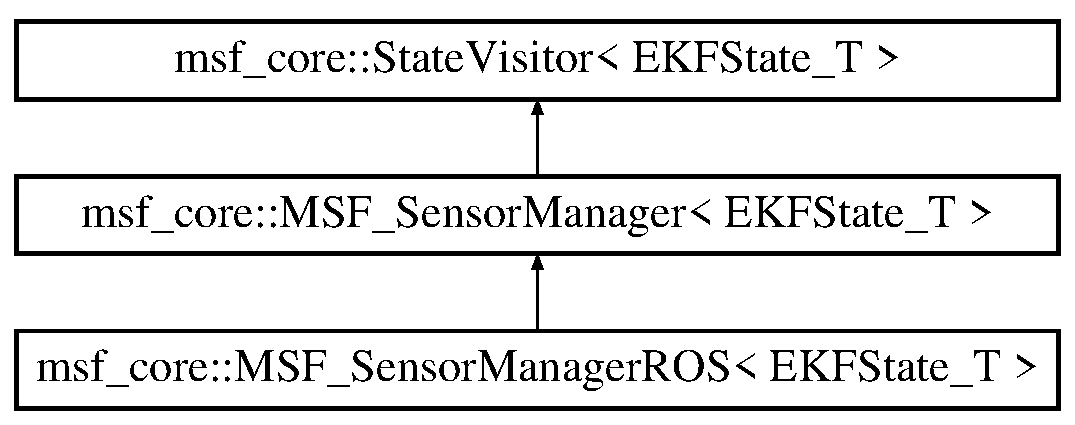
\includegraphics[height=3.000000cm]{classmsf__core_1_1StateVisitor}
\end{center}
\end{figure}
\subsection*{Public Member Functions}
\begin{DoxyCompactItemize}
\item 
\hypertarget{classmsf__core_1_1StateVisitor_a42a37cdfe7b7c4aa5d3c9f5f661ab581}{virtual void \hyperlink{classmsf__core_1_1StateVisitor_a42a37cdfe7b7c4aa5d3c9f5f661ab581}{reset\-State} (E\-K\-F\-State\-\_\-\-T \&state) const =0}\label{classmsf__core_1_1StateVisitor_a42a37cdfe7b7c4aa5d3c9f5f661ab581}

\begin{DoxyCompactList}\small\item\em The state is set to zero/identity, this method will be called to give the user the possibility to change the reset values of some states. \end{DoxyCompactList}\end{DoxyCompactItemize}


\subsection{Detailed Description}
\subsubsection*{template$<$typename E\-K\-F\-State\-\_\-\-T$>$class msf\-\_\-core\-::\-State\-Visitor$<$ E\-K\-F\-State\-\_\-\-T $>$}

Visitor pattern to allow the user to set state init values. 

The documentation for this class was generated from the following file\-:\begin{DoxyCompactItemize}
\item 
msf\-\_\-core/include/msf\-\_\-core/msf\-\_\-statevisitor.\-h\end{DoxyCompactItemize}

\hypertarget{structmsf__tmp_1_1StripConstPtr}{\section{msf\-\_\-tmp\-:\-:Strip\-Const\-Ptr$<$ T $>$ Struct Template Reference}
\label{structmsf__tmp_1_1StripConstPtr}\index{msf\-\_\-tmp\-::\-Strip\-Const\-Ptr$<$ T $>$@{msf\-\_\-tmp\-::\-Strip\-Const\-Ptr$<$ T $>$}}
}
\subsection*{Public Types}
\begin{DoxyCompactItemize}
\item 
\hypertarget{structmsf__tmp_1_1StripConstPtr_aaa6063832bdfda3b18f09e719a9f0626}{typedef T {\bfseries result\-\_\-t}}\label{structmsf__tmp_1_1StripConstPtr_aaa6063832bdfda3b18f09e719a9f0626}

\end{DoxyCompactItemize}


The documentation for this struct was generated from the following file\-:\begin{DoxyCompactItemize}
\item 
msf\-\_\-core/include/msf\-\_\-core/msf\-\_\-typetraits.\-hpp\end{DoxyCompactItemize}

\hypertarget{structmsf__tmp_1_1StripConstPtr_3_01const_01T_01_5_01_4}{\section{msf\-\_\-tmp\-:\-:Strip\-Const\-Ptr$<$ const T $\ast$ $>$ Struct Template Reference}
\label{structmsf__tmp_1_1StripConstPtr_3_01const_01T_01_5_01_4}\index{msf\-\_\-tmp\-::\-Strip\-Const\-Ptr$<$ const T $\ast$ $>$@{msf\-\_\-tmp\-::\-Strip\-Const\-Ptr$<$ const T $\ast$ $>$}}
}
\subsection*{Public Types}
\begin{DoxyCompactItemize}
\item 
\hypertarget{structmsf__tmp_1_1StripConstPtr_3_01const_01T_01_5_01_4_abd775b4e0a2c4592dbbb4c7cc6910535}{typedef T {\bfseries result\-\_\-t}}\label{structmsf__tmp_1_1StripConstPtr_3_01const_01T_01_5_01_4_abd775b4e0a2c4592dbbb4c7cc6910535}

\end{DoxyCompactItemize}


The documentation for this struct was generated from the following file\-:\begin{DoxyCompactItemize}
\item 
msf\-\_\-core/include/msf\-\_\-core/msf\-\_\-typetraits.\-hpp\end{DoxyCompactItemize}

\hypertarget{structmsf__tmp_1_1StripConstPtr_3_01const_01T_01_4}{\section{msf\-\_\-tmp\-:\-:Strip\-Const\-Ptr$<$ const T $>$ Struct Template Reference}
\label{structmsf__tmp_1_1StripConstPtr_3_01const_01T_01_4}\index{msf\-\_\-tmp\-::\-Strip\-Const\-Ptr$<$ const T $>$@{msf\-\_\-tmp\-::\-Strip\-Const\-Ptr$<$ const T $>$}}
}


{\ttfamily \#include $<$msf\-\_\-typetraits.\-hpp$>$}

\subsection*{Public Types}
\begin{DoxyCompactItemize}
\item 
typedef T \hyperlink{structmsf__tmp_1_1StripConstPtr_3_01const_01T_01_4_a1c31b8f2ab8c3e038d6c0e1cd5857d18}{result\-\_\-t}
\end{DoxyCompactItemize}


\subsection{Member Typedef Documentation}
\hypertarget{structmsf__tmp_1_1StripConstPtr_3_01const_01T_01_4_a1c31b8f2ab8c3e038d6c0e1cd5857d18}{\index{msf\-\_\-tmp\-::\-Strip\-Const\-Ptr$<$ const T $>$@{msf\-\_\-tmp\-::\-Strip\-Const\-Ptr$<$ const T $>$}!result\-\_\-t@{result\-\_\-t}}
\index{result\-\_\-t@{result\-\_\-t}!msf_tmp::StripConstPtr< const T >@{msf\-\_\-tmp\-::\-Strip\-Const\-Ptr$<$ const T $>$}}
\subsubsection[{result\-\_\-t}]{\setlength{\rightskip}{0pt plus 5cm}template$<$typename T $>$ typedef T {\bf msf\-\_\-tmp\-::\-Strip\-Const\-Ptr}$<$ const T $>$\-::{\bf result\-\_\-t}}}\label{structmsf__tmp_1_1StripConstPtr_3_01const_01T_01_4_a1c31b8f2ab8c3e038d6c0e1cd5857d18}


The documentation for this struct was generated from the following file\-:\begin{DoxyCompactItemize}
\item 
msf\-\_\-core/include/msf\-\_\-core/\hyperlink{msf__typetraits_8hpp}{msf\-\_\-typetraits.\-hpp}\end{DoxyCompactItemize}

\hypertarget{structmsf__tmp_1_1StripConstPtr_3_01T_01_5_01_4}{\section{msf\-\_\-tmp\-:\-:Strip\-Const\-Ptr$<$ T $\ast$ $>$ Struct Template Reference}
\label{structmsf__tmp_1_1StripConstPtr_3_01T_01_5_01_4}\index{msf\-\_\-tmp\-::\-Strip\-Const\-Ptr$<$ T $\ast$ $>$@{msf\-\_\-tmp\-::\-Strip\-Const\-Ptr$<$ T $\ast$ $>$}}
}


{\ttfamily \#include $<$msf\-\_\-typetraits.\-hpp$>$}

\subsection*{Public Types}
\begin{DoxyCompactItemize}
\item 
typedef T \hyperlink{structmsf__tmp_1_1StripConstPtr_3_01T_01_5_01_4_a488d62f2859f809b9dc13e5e99a81582}{result\-\_\-t}
\end{DoxyCompactItemize}


\subsection{Member Typedef Documentation}
\hypertarget{structmsf__tmp_1_1StripConstPtr_3_01T_01_5_01_4_a488d62f2859f809b9dc13e5e99a81582}{\index{msf\-\_\-tmp\-::\-Strip\-Const\-Ptr$<$ T $\ast$ $>$@{msf\-\_\-tmp\-::\-Strip\-Const\-Ptr$<$ T $\ast$ $>$}!result\-\_\-t@{result\-\_\-t}}
\index{result\-\_\-t@{result\-\_\-t}!msf_tmp::StripConstPtr< T * >@{msf\-\_\-tmp\-::\-Strip\-Const\-Ptr$<$ T $\ast$ $>$}}
\subsubsection[{result\-\_\-t}]{\setlength{\rightskip}{0pt plus 5cm}template$<$typename T $>$ typedef T {\bf msf\-\_\-tmp\-::\-Strip\-Const\-Ptr}$<$ T $\ast$ $>$\-::{\bf result\-\_\-t}}}\label{structmsf__tmp_1_1StripConstPtr_3_01T_01_5_01_4_a488d62f2859f809b9dc13e5e99a81582}


The documentation for this struct was generated from the following file\-:\begin{DoxyCompactItemize}
\item 
msf\-\_\-core/include/msf\-\_\-core/\hyperlink{msf__typetraits_8hpp}{msf\-\_\-typetraits.\-hpp}\end{DoxyCompactItemize}

\hypertarget{structmsf__tmp_1_1StripConstReference}{\section{msf\-\_\-tmp\-:\-:Strip\-Const\-Reference$<$ T $>$ Struct Template Reference}
\label{structmsf__tmp_1_1StripConstReference}\index{msf\-\_\-tmp\-::\-Strip\-Const\-Reference$<$ T $>$@{msf\-\_\-tmp\-::\-Strip\-Const\-Reference$<$ T $>$}}
}


{\ttfamily \#include $<$msf\-\_\-typetraits.\-hpp$>$}

\subsection*{Public Types}
\begin{DoxyCompactItemize}
\item 
typedef T \hyperlink{structmsf__tmp_1_1StripConstReference_a4069e12bbcefd7f81f4596cee921b0df}{result\-\_\-t}
\end{DoxyCompactItemize}


\subsection{Member Typedef Documentation}
\hypertarget{structmsf__tmp_1_1StripConstReference_a4069e12bbcefd7f81f4596cee921b0df}{\index{msf\-\_\-tmp\-::\-Strip\-Const\-Reference@{msf\-\_\-tmp\-::\-Strip\-Const\-Reference}!result\-\_\-t@{result\-\_\-t}}
\index{result\-\_\-t@{result\-\_\-t}!msf_tmp::StripConstReference@{msf\-\_\-tmp\-::\-Strip\-Const\-Reference}}
\subsubsection[{result\-\_\-t}]{\setlength{\rightskip}{0pt plus 5cm}template$<$typename T$>$ typedef T {\bf msf\-\_\-tmp\-::\-Strip\-Const\-Reference}$<$ T $>$\-::{\bf result\-\_\-t}}}\label{structmsf__tmp_1_1StripConstReference_a4069e12bbcefd7f81f4596cee921b0df}


The documentation for this struct was generated from the following file\-:\begin{DoxyCompactItemize}
\item 
msf\-\_\-core/include/msf\-\_\-core/\hyperlink{msf__typetraits_8hpp}{msf\-\_\-typetraits.\-hpp}\end{DoxyCompactItemize}

\hypertarget{structmsf__tmp_1_1StripConstReference_3_01const_01T_01_6_01_4}{\section{msf\-\_\-tmp\-:\-:Strip\-Const\-Reference$<$ const T \& $>$ Struct Template Reference}
\label{structmsf__tmp_1_1StripConstReference_3_01const_01T_01_6_01_4}\index{msf\-\_\-tmp\-::\-Strip\-Const\-Reference$<$ const T \& $>$@{msf\-\_\-tmp\-::\-Strip\-Const\-Reference$<$ const T \& $>$}}
}
\subsection*{Public Types}
\begin{DoxyCompactItemize}
\item 
\hypertarget{structmsf__tmp_1_1StripConstReference_3_01const_01T_01_6_01_4_a2535057bb12b6b644caf7a8e2b4059c6}{typedef T {\bfseries result\-\_\-t}}\label{structmsf__tmp_1_1StripConstReference_3_01const_01T_01_6_01_4_a2535057bb12b6b644caf7a8e2b4059c6}

\end{DoxyCompactItemize}


The documentation for this struct was generated from the following file\-:\begin{DoxyCompactItemize}
\item 
msf\-\_\-core/include/msf\-\_\-core/msf\-\_\-typetraits.\-hpp\end{DoxyCompactItemize}

\hypertarget{structmsf__tmp_1_1StripConstReference_3_01const_01T_01_4}{\section{msf\-\_\-tmp\-:\-:Strip\-Const\-Reference$<$ const T $>$ Struct Template Reference}
\label{structmsf__tmp_1_1StripConstReference_3_01const_01T_01_4}\index{msf\-\_\-tmp\-::\-Strip\-Const\-Reference$<$ const T $>$@{msf\-\_\-tmp\-::\-Strip\-Const\-Reference$<$ const T $>$}}
}


{\ttfamily \#include $<$msf\-\_\-typetraits.\-hpp$>$}

\subsection*{Public Types}
\begin{DoxyCompactItemize}
\item 
typedef T \hyperlink{structmsf__tmp_1_1StripConstReference_3_01const_01T_01_4_a37e22d99853f07caf2ae4ef4455e3d16}{result\-\_\-t}
\end{DoxyCompactItemize}


\subsection{Member Typedef Documentation}
\hypertarget{structmsf__tmp_1_1StripConstReference_3_01const_01T_01_4_a37e22d99853f07caf2ae4ef4455e3d16}{\index{msf\-\_\-tmp\-::\-Strip\-Const\-Reference$<$ const T $>$@{msf\-\_\-tmp\-::\-Strip\-Const\-Reference$<$ const T $>$}!result\-\_\-t@{result\-\_\-t}}
\index{result\-\_\-t@{result\-\_\-t}!msf_tmp::StripConstReference< const T >@{msf\-\_\-tmp\-::\-Strip\-Const\-Reference$<$ const T $>$}}
\subsubsection[{result\-\_\-t}]{\setlength{\rightskip}{0pt plus 5cm}template$<$typename T $>$ typedef T {\bf msf\-\_\-tmp\-::\-Strip\-Const\-Reference}$<$ const T $>$\-::{\bf result\-\_\-t}}}\label{structmsf__tmp_1_1StripConstReference_3_01const_01T_01_4_a37e22d99853f07caf2ae4ef4455e3d16}


The documentation for this struct was generated from the following file\-:\begin{DoxyCompactItemize}
\item 
msf\-\_\-core/include/msf\-\_\-core/\hyperlink{msf__typetraits_8hpp}{msf\-\_\-typetraits.\-hpp}\end{DoxyCompactItemize}

\hypertarget{structmsf__tmp_1_1StripConstReference_3_01T_01_6_01_4}{\section{msf\-\_\-tmp\-:\-:Strip\-Const\-Reference$<$ T \& $>$ Struct Template Reference}
\label{structmsf__tmp_1_1StripConstReference_3_01T_01_6_01_4}\index{msf\-\_\-tmp\-::\-Strip\-Const\-Reference$<$ T \& $>$@{msf\-\_\-tmp\-::\-Strip\-Const\-Reference$<$ T \& $>$}}
}


{\ttfamily \#include $<$msf\-\_\-typetraits.\-hpp$>$}

\subsection*{Public Types}
\begin{DoxyCompactItemize}
\item 
typedef T \hyperlink{structmsf__tmp_1_1StripConstReference_3_01T_01_6_01_4_ae467d3d062236fe36daa8c856cee2741}{result\-\_\-t}
\end{DoxyCompactItemize}


\subsection{Member Typedef Documentation}
\hypertarget{structmsf__tmp_1_1StripConstReference_3_01T_01_6_01_4_ae467d3d062236fe36daa8c856cee2741}{\index{msf\-\_\-tmp\-::\-Strip\-Const\-Reference$<$ T \& $>$@{msf\-\_\-tmp\-::\-Strip\-Const\-Reference$<$ T \& $>$}!result\-\_\-t@{result\-\_\-t}}
\index{result\-\_\-t@{result\-\_\-t}!msf_tmp::StripConstReference< T & >@{msf\-\_\-tmp\-::\-Strip\-Const\-Reference$<$ T \& $>$}}
\subsubsection[{result\-\_\-t}]{\setlength{\rightskip}{0pt plus 5cm}template$<$typename T $>$ typedef T {\bf msf\-\_\-tmp\-::\-Strip\-Const\-Reference}$<$ T \& $>$\-::{\bf result\-\_\-t}}}\label{structmsf__tmp_1_1StripConstReference_3_01T_01_6_01_4_ae467d3d062236fe36daa8c856cee2741}


The documentation for this struct was generated from the following file\-:\begin{DoxyCompactItemize}
\item 
msf\-\_\-core/include/msf\-\_\-core/\hyperlink{msf__typetraits_8hpp}{msf\-\_\-typetraits.\-hpp}\end{DoxyCompactItemize}

\hypertarget{structmsf__tmp_1_1StripReference}{\section{msf\-\_\-tmp\-:\-:Strip\-Reference$<$ T $>$ Struct Template Reference}
\label{structmsf__tmp_1_1StripReference}\index{msf\-\_\-tmp\-::\-Strip\-Reference$<$ T $>$@{msf\-\_\-tmp\-::\-Strip\-Reference$<$ T $>$}}
}


{\ttfamily \#include $<$msf\-\_\-typetraits.\-hpp$>$}

\subsection*{Public Types}
\begin{DoxyCompactItemize}
\item 
typedef T \hyperlink{structmsf__tmp_1_1StripReference_a3e5488373eb6358b4b30fc3386bb50a5}{result\-\_\-t}
\end{DoxyCompactItemize}


\subsection{Member Typedef Documentation}
\hypertarget{structmsf__tmp_1_1StripReference_a3e5488373eb6358b4b30fc3386bb50a5}{\index{msf\-\_\-tmp\-::\-Strip\-Reference@{msf\-\_\-tmp\-::\-Strip\-Reference}!result\-\_\-t@{result\-\_\-t}}
\index{result\-\_\-t@{result\-\_\-t}!msf_tmp::StripReference@{msf\-\_\-tmp\-::\-Strip\-Reference}}
\subsubsection[{result\-\_\-t}]{\setlength{\rightskip}{0pt plus 5cm}template$<$typename T $>$ typedef T {\bf msf\-\_\-tmp\-::\-Strip\-Reference}$<$ T $>$\-::{\bf result\-\_\-t}}}\label{structmsf__tmp_1_1StripReference_a3e5488373eb6358b4b30fc3386bb50a5}


The documentation for this struct was generated from the following file\-:\begin{DoxyCompactItemize}
\item 
msf\-\_\-core/include/msf\-\_\-core/\hyperlink{msf__typetraits_8hpp}{msf\-\_\-typetraits.\-hpp}\end{DoxyCompactItemize}

\hypertarget{structmsf__tmp_1_1StripReference_3_01const_01T_01_6_01_4}{\section{msf\-\_\-tmp\-:\-:Strip\-Reference$<$ const T \& $>$ Struct Template Reference}
\label{structmsf__tmp_1_1StripReference_3_01const_01T_01_6_01_4}\index{msf\-\_\-tmp\-::\-Strip\-Reference$<$ const T \& $>$@{msf\-\_\-tmp\-::\-Strip\-Reference$<$ const T \& $>$}}
}
\subsection*{Public Types}
\begin{DoxyCompactItemize}
\item 
\hypertarget{structmsf__tmp_1_1StripReference_3_01const_01T_01_6_01_4_a3f0da0790a8e34e58f4961f09c76a840}{typedef const T {\bfseries result\-\_\-t}}\label{structmsf__tmp_1_1StripReference_3_01const_01T_01_6_01_4_a3f0da0790a8e34e58f4961f09c76a840}

\end{DoxyCompactItemize}


The documentation for this struct was generated from the following file\-:\begin{DoxyCompactItemize}
\item 
msf\-\_\-core/include/msf\-\_\-core/msf\-\_\-typetraits.\-hpp\end{DoxyCompactItemize}

\hypertarget{structmsf__tmp_1_1StripReference_3_01const_01T_01_4}{\section{msf\-\_\-tmp\-:\-:Strip\-Reference$<$ const T $>$ Struct Template Reference}
\label{structmsf__tmp_1_1StripReference_3_01const_01T_01_4}\index{msf\-\_\-tmp\-::\-Strip\-Reference$<$ const T $>$@{msf\-\_\-tmp\-::\-Strip\-Reference$<$ const T $>$}}
}


{\ttfamily \#include $<$msf\-\_\-typetraits.\-hpp$>$}

\subsection*{Public Types}
\begin{DoxyCompactItemize}
\item 
typedef const T \hyperlink{structmsf__tmp_1_1StripReference_3_01const_01T_01_4_a4aa9040c1a950280fc8a134e0f7b6e4a}{result\-\_\-t}
\end{DoxyCompactItemize}


\subsection{Member Typedef Documentation}
\hypertarget{structmsf__tmp_1_1StripReference_3_01const_01T_01_4_a4aa9040c1a950280fc8a134e0f7b6e4a}{\index{msf\-\_\-tmp\-::\-Strip\-Reference$<$ const T $>$@{msf\-\_\-tmp\-::\-Strip\-Reference$<$ const T $>$}!result\-\_\-t@{result\-\_\-t}}
\index{result\-\_\-t@{result\-\_\-t}!msf_tmp::StripReference< const T >@{msf\-\_\-tmp\-::\-Strip\-Reference$<$ const T $>$}}
\subsubsection[{result\-\_\-t}]{\setlength{\rightskip}{0pt plus 5cm}template$<$typename T $>$ typedef const T {\bf msf\-\_\-tmp\-::\-Strip\-Reference}$<$ const T $>$\-::{\bf result\-\_\-t}}}\label{structmsf__tmp_1_1StripReference_3_01const_01T_01_4_a4aa9040c1a950280fc8a134e0f7b6e4a}


The documentation for this struct was generated from the following file\-:\begin{DoxyCompactItemize}
\item 
msf\-\_\-core/include/msf\-\_\-core/\hyperlink{msf__typetraits_8hpp}{msf\-\_\-typetraits.\-hpp}\end{DoxyCompactItemize}

\hypertarget{structmsf__tmp_1_1StripReference_3_01T_01_6_01_4}{\section{msf\-\_\-tmp\-:\-:Strip\-Reference$<$ T \& $>$ Struct Template Reference}
\label{structmsf__tmp_1_1StripReference_3_01T_01_6_01_4}\index{msf\-\_\-tmp\-::\-Strip\-Reference$<$ T \& $>$@{msf\-\_\-tmp\-::\-Strip\-Reference$<$ T \& $>$}}
}


{\ttfamily \#include $<$msf\-\_\-typetraits.\-hpp$>$}

\subsection*{Public Types}
\begin{DoxyCompactItemize}
\item 
typedef T \hyperlink{structmsf__tmp_1_1StripReference_3_01T_01_6_01_4_a3c52c9c3462d4be0736e5820c2121b68}{result\-\_\-t}
\end{DoxyCompactItemize}


\subsection{Member Typedef Documentation}
\hypertarget{structmsf__tmp_1_1StripReference_3_01T_01_6_01_4_a3c52c9c3462d4be0736e5820c2121b68}{\index{msf\-\_\-tmp\-::\-Strip\-Reference$<$ T \& $>$@{msf\-\_\-tmp\-::\-Strip\-Reference$<$ T \& $>$}!result\-\_\-t@{result\-\_\-t}}
\index{result\-\_\-t@{result\-\_\-t}!msf_tmp::StripReference< T & >@{msf\-\_\-tmp\-::\-Strip\-Reference$<$ T \& $>$}}
\subsubsection[{result\-\_\-t}]{\setlength{\rightskip}{0pt plus 5cm}template$<$typename T $>$ typedef T {\bf msf\-\_\-tmp\-::\-Strip\-Reference}$<$ T \& $>$\-::{\bf result\-\_\-t}}}\label{structmsf__tmp_1_1StripReference_3_01T_01_6_01_4_a3c52c9c3462d4be0736e5820c2121b68}


The documentation for this struct was generated from the following file\-:\begin{DoxyCompactItemize}
\item 
msf\-\_\-core/include/msf\-\_\-core/\hyperlink{msf__typetraits_8hpp}{msf\-\_\-typetraits.\-hpp}\end{DoxyCompactItemize}

\printindex
\end{document}
